%\documentclass[12pt,twoside]{book}
\documentclass[12pt,twoside,openany]{book}



%%%%%%%%%%%%%%%%%%%%%%%%%%%%%%%%%%%%%%%%%%%%%%%
% Encoding and language

\usepackage[T1]{fontenc}
\usepackage[utf8]{inputenc}
\usepackage[english]{babel}





%%%%%%%%%%%%%%%%%%%%%%%%%%%%%%%%%%%%%%%%%%%%%%%
% Layout

\usepackage[a4paper,top=2cm,bottom=2cm,left=2cm,right=2cm]{geometry}
\usepackage{setspace}
\usepackage{enumitem}




%%%%%%%%%%%%%%%%%%%%%%%%%%%%%%%%%%%%%%%%%%%%%%%
% Mathematics

\usepackage{amsmath,amssymb,amsthm,mathtools}
\usepackage{cancel}





%%%%%%%%%%%%%%%%%%%%%%%%%%%%%%%%%%%%%%%%%%%%%%%
% Graphics and tables

\usepackage{graphicx}
\usepackage{float}
\usepackage{placeins}
\usepackage{caption}
\usepackage{subcaption}
\usepackage{booktabs}

\graphicspath{{Thesis_images/}}



%%%%%%%%%%%%%%%%%%%%%%%%%%%%%%%%%%%%%%%%%%%%%%%
% Boxes

%\usepackage{tcolorbox}





%%%%%%%%%%%%%%%%%%%%%%%%%%%%%%%%%%%%%%%%%%%%%%%
% Header / Footer

\usepackage{fancyhdr}

\pagestyle{fancy}
\fancyhf{}

\setlength{\headheight}{15pt}

\fancyhead[LE]{\thepage}
\fancyhead[RO]{\thepage}
\fancyhead[RE]{\nouppercase{\leftmark}}
\fancyhead[LO]{\nouppercase{\rightmark}}

\renewcommand{\headrulewidth}{0.4pt}
\renewcommand{\footrulewidth}{0pt}



\fancypagestyle{plain}{
  \fancyhf{}                      % pulisce tutto

  \fancyfoot[C]{\thepage}         % numero centrato in basso

  \renewcommand{\headrulewidth}{0pt}
  \renewcommand{\footrulewidth}{0pt}
}










%%%%%%%%%%%%%%%%%%%%%%%%%%%%%%%%%%%%%%%%%%%%%%%
% Hyperref (sempre quasi alla fine)

\usepackage{hyperref}






%%%%%%%%%%%%%%%%%%%%%%%%%%%%%%%%%%%%%%%%%%%%%%%
% Bibliography

\usepackage{csquotes}
\usepackage[
  backend=biber,
  style=authoryear,
  maxcitenames=2,
  mincitenames=1,
  maxbibnames=3
]{biblatex}
\addbibresource{bibliografia.bib}




%%%%%%%%%%%%%%%%%%%%%%%%%%%%%%%%%%%%%%%%
% Contents

\usepackage{tocloft}
\renewcommand{\cftchapaftersnum}{\space}
\renewcommand{\cftchapnumwidth}{8em}
\renewcommand{\cftchappresnum}{CHAPTER.~}






%%%%%%%%%%%%%%%%%%%%%%%%%%%%%%%%%%%%%%%%%
% Chapters Layout

\usepackage{titlesec}

\titleformat{\chapter}[display]
  {\centering}                % allineamento
  {\Huge\thechapter}          % numero capitolo
  {1ex}                       % spazio tra numero e titolo
  {\Large\scshape}            % stile titolo
  [\vspace{1ex}\rule{1.0\textwidth}{0.4pt}]  % linea sotto





%%%%%%%%%%%%%%%%%%%%%%%%%%%%%%%%%%%%%%%%%%
% Enumeration style

\renewcommand{\thesection}{\arabic{chapter}.\arabic{section}}





%%%%%%%%%%%%%%%%%%%%%%%%%%%%%%%%%%%%%%%%%
% border issues









%%%%%%%%%%%%%%%%%%%%%%%%%%%%%%%%%%%%%%%%%%%%%%%
%%%%%%%%%%%%%%%%%%%%%%%%%%%%%%%%%%%%%%%%%%%%%%%

%\includeonly{Chapter_1}

%\includeonly{Chapter_2}

%\includeonly{Chapter_3}

%%%%%%%%%%%%%%%%%%%%%%%%%%%%%%%%%%%%%%%%%%%%%%%
%%%%%%%%%%%%%%%%%%%%%%%%%%%%%%%%%%%%%%%%%%%%%%%





\begin{document}



\pagestyle{empty}

\begin{center}
    {\Large\bfseries Abstract}
\end{center}

\vspace{1cm}
\noindent
The next generation of gravitational-wave (GW) observatories, Laser Interferometer Space Antenna (LISA) and the Einstein Telescope (ET), will jointly probe compact objects with masses ranging from a few to $\sim 10^7\,M_\odot$ over the frequency interval extending from $10^{-4}$ to $10^{4}\,\mathrm{Hz}$. This unprecedented observational window makes it essential to identify promising GW sources, investigate their formation channels, and characterize the physical properties of the emitted signals.\\Among the most compelling candidates are binaries hosting intermediate-mass black holes (IMBHs), whose inspiral GW emission would offer unique insights into this still poorly constrained population of massive black holes (MBHs). Empirical scaling relations suggest that IMBHs preferentially reside in the nuclei of low-mass and dwarf galaxies. Unlike their massive counterparts, these systems display a wide variety of structural and kinematical properties, potentially giving rise to quite different evolutionary pathways toward binary coalescence.\\This thesis investigates the dynamical evolution of IMBH binaries, with particular emphasis on the coalescence timescale and the evolution of the binary separation and eccentricity. To this end, both the Quinlan--Sesana hybrid model and Ketju direct N-body simulations are employed. While the former approach provides an efficient framework for reconstructing the evolution of BH binaries once the stellar background properties and the binary initial conditions are specified, the Ketju module, implemented into GADGET-4, models SMBHs and stars as point particles during close encounters through an algorithmically regularized integrator, thereby accurately capturing the orbital decay driven by stellar scattering with unprecedented spatial resolution from the merger of the host galaxies to the final coalescence.\\The analysis explores different stellar backgrounds, including nucleated dwarf galaxies and observationally motivated high-redshift galaxy models with enhanced stellar densities resulting from cosmic size evolution. The results confirm that IMBH binaries embedded in nucleated dwarf galaxies can merge within a few Myr. More remarkably, they show that even non-nucleated high-redshift galaxies may drive binary coalescence within a Hubble time, identifying these systems as promising sources of detectable gravitational waves. Finally, the reconstructed binary evolution is finally exploited to compute the associated GW signals, providing observational predictions for the LISA and Einstein Telescope era.



\clearpage





\tableofcontents





%%%%%%%%%%%%%%%%%%%%%%%%%%%%%%

\pagestyle{fancy}

%%%%%%%%%%%%%%%%%%%%%%%%%%%%%%

\chapter*{Introduction}
\addcontentsline{toc}{chapter}{Introduction}


Massive black holes play a fundamental role in the formation and evolution of galaxies. Observations have established that they are ubiquitously found at the centers of nearby galaxies \parencite{Kormendy_1995}, while tight empirical correlations between their masses and the properties of the host galactic bulges suggest a close co-evolution of black holes and galaxies \parencite{Magorrian_1998}.
MBHs are belived to be common in galaxy centres at all cosmic epochs; a piece of evidence for their existence, from low to high redshift, comes from the transient activity of galactic nuclei (AGN) over the hosts lifetime (see, e.g., \textcite{Jahnke_2025}).\\Black holes (BHs) span a wide range of masses $(\sim 10-10^{9}\,M_\odot)$ and various formation models have been proposed based on their mass. At the two extremes of the black-hole mass spectrum lie stellar-mass black holes and supermassive black holes (SMBHs). Stellar evolution theory predicts that stellar-mass BHs may be the remnants of massive stars with either Zero Age Main Sequence mass $M_{ZAMS}\lesssim 140\,M_\odot$ or $M_{ZAMS}\gtrsim 260\,M_\odot$; otherwise, they undergo fully disruption and end their life as Pair Instability Super Novae \parencite{Farmer_2019}. In recent years, the properties of this population have been significantly constrained through the detection of gravitational waves (GWs) from merging compact binaries \parencite{Abbott_2016}, as well as by advances in microlensing techniques capable of identifying isolated BH candidates \parencite{Bennett_2002}.
On the opposite side $(\sim 10^6-10^9\,M_\odot)$, instead, Pulsar timing arrays has already probed the upper mass range of SMBHs population \parencite{Taylor_2021}, whose most accepted formation model interpret them as the final stage of a secular accretion onto initially lighter black hole seeds.\\While substantial progress has been made in detecting and characterizing both stellar-mass BHs and SMBHs, the observational confirmation and detailed investigation of intermediate-mass black holes (IMBHs), spanning the mass range $\sim 10^2$--$10^5,M_\odot$, remain significantly more challenging. Although an increasing number of candidates have been identified in the local Universe, particularly in dwarf galaxies, through accretion signatures (see, e.g., \textcite{Reines_2013}), their sphere of influence—conventionally defined as the radius enclosing a stellar mass equal to twice that of the central BH \parencite{Sesana_2015}, within which the BH gravitational potential dominates—is typically too small for reliable stellar or gas dynamical measurements, especially at higher redshift. Nevertheless, the discovery of high-redshift quasars (see, e.g., \textcite{Banados_2018}) points to the existence of BH seeds with masses comparable to those of IMBHs already in the early Universe and motivates the common practice of inferring the presence of IMBHs by extrapolating the empirical correlation between BH mass and the stellar bulge mass of the host galaxy \parencite{Schutte_2019}.\\Figure \ref{IMBH_Pathways} illustrates three distinct theoretical pathways for IMBH formation, highlighting the number of BHs expected to form through each channel, their corresponding mass ranges, and the redshift range over which each formation mechanism is expected to be most efficient. Each formation channel is expected to proceed as follows:
\begin{itemize}
 \item Sufficiently massive primordial stars, commonly referred to as Population III (Pop III) stars, may possess enough gravitational binding energy to withstand the energy released during the photodisintegration-induced collapse of their cores, ultimately leading to the formation of a BH remnant \parencite{Fryer_2001}.
 \item At high redshift, metal-free gas clouds may undergo nearly monolithic gravitational collapse without significant fragmentation, in contrast to what is typically observed in the present-day Universe, owing to the inefficient cooling of neutral hydrogen and lead to the formation of IMBHs \parencite{Lodato_2006}.
 \item Runaway stellar collisions in high-density clusters may trigger a sequence of stellar mergers, progressively producing more massive stars that can undergo further collisions. The final product of this repeated merger process may eventually collapse into an IMBH (see, e.g., \textcite{Rodriguez_2019}; \textcite{Devecchi_2009}).
\end{itemize}
\begin{figure}[H]
    \centering
    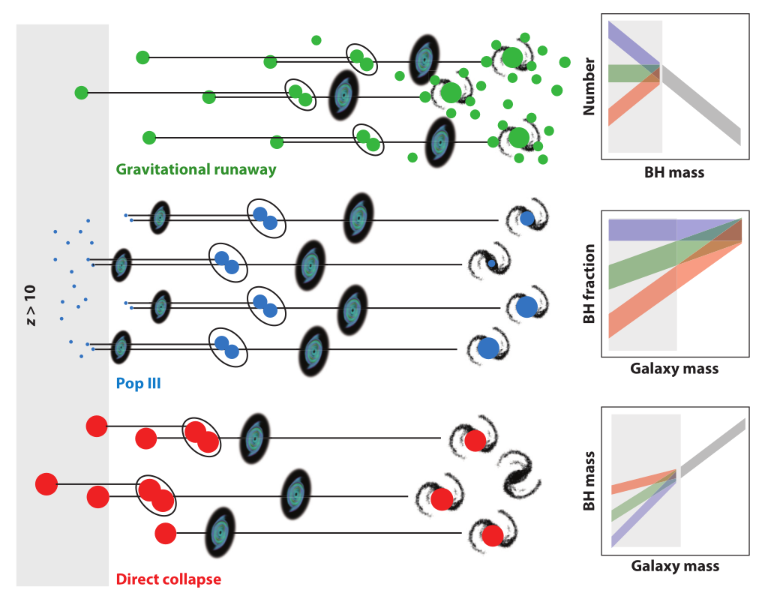
\includegraphics[width=0.5\linewidth]{IMBH_Review_Formation.png}
    \caption{Schematic representation of different BH seeding channels, from their formation and subsequent growth through mergers and accretion to the present day: Pop III stars (blue), direct collapse (red), and gravitational runaway (green). The corresponding present-day BH mass functions, occupation fractions, and BH–galaxy scaling relations are shown on the right. Picture from \textcite{Greene_2020}.}
    \label{IMBH_Pathways}
\end{figure}
Within the framework of galaxy hierarchical growth scenario (see, e.g., \textcite{White_1978}; SESANA2020), the creation of massive black hole binaries (MBHBs) is expected to occur, over cosmic time, as a natural consequence of mergers of possible hosts:


between galaxies. These systems are among the most powerful emitters of gravitational waves (GWs) in the universe, making them prime targets for detection with current and future GW observatories.\\Although the merger rate of low mass galaxies has not been well determined yet, the interaction and merging of these structures should lead to the formation of IMBH-IMBH binaries. The upcoming Laser Interferometer Space Antenna (LISA), a joint ESA/NASA space mission, promises to demystify IMBHs, being sensitive to GW signals, from $\sim 10^{-4}$ Hz to $\sim 10^{-1}$ Hz, produced at late stage of the merger \parencite{Amaro-Seoane_2017}; their masses, within $10^4-10^7\,M_\odot$, and redshift will be estimated out to $z=20$ with very high precision \parencite{Colpi_2024}.\\Despite dwarf galaxies have been identified at incredibly high redshift \parencite{Kikuchihara_2020}, hence opening to the possibility of reciving GW signals from merging IMBH binaries if this process takes place within the Hubble time, numerical simulations \parencite{Khan_2024} proved that in non-nucleated dwarfs the low stellar density in the central regions results in inefficient hardening and stalling of the binary. However, the vast majority of galaxies with stellar mass $10^8-10^{11}\,M_\odot$ harbor a nuclear star cluster (NSC), an extraordinarily dense and dynamically distinct stellar assembly, in their innermost regions; the existence of a such dense envirnoment inside dwarf galaxies, as reported by e.g. \textcite{Nguyen_2018}, may drastically reduce the coalescence time of the IMBH pair.\\This thesis work is aimed at studying the evolution of the main orbital parameters of the binary, with focus on semimajor axis $a$ and eccentricity $e$, and analyzing how the variation of BHs masses, host galaxy properties and IC of the binary, i.e. $(a_0,e_0)$ impacts , impact its evolution and coalescence time. In this spirit, the study combines a self-consistent hybrid model developed by \textcite{Sesana_2010} with N-body simulations performed using the KETJU code \parencite{Mannerkoski_2023}, which will be described in more detail later.\\The structure of this thesis is outlined as follows.\\In \autoref{chap:chapter1}, we provide a brief overview of the main physical mechanisms responsible for the BH binary shrinking; this includes dynamical friction, stellar scattering processes and GWs emission,which dominates the late stages of the inspiral.\\In \autoref{chap:chapter2}, we introduce the self-consistent hybrid model developed by \textcite{Quinlan_1996} and \textcite{Sesana_2010}; it is thus applied to a sample of galaxies and exploring the parameters space in order to emphasise how different environmental and initial conditions lead to different binary evolution.\\In \autoref{chap:chapter3} we describe the main features of the codes used to generate N-body initial condition and N-body numerical simulations and compare the obtained binary evolutionary tracks with those of the previous chapter.\\Finally, the main results of this work are summarized, and possible future improvements are reported in the concluding chapter.
%\clearpage






 
%%%%%%%%%%%%%%%%%%%%%%%%%%%%%%%%%%%%%%


%\include{Chapter_1}


%%%%%%%%%%%%%%%%%%%%%%%%%%%%%%%%%%%%%%







\chapter{Physical Mechanisms of Binary Hardening}\label{chap:chapter1}




\vspace*{\fill}

\begin{center}
\begin{minipage}{0.65\textwidth}
\centering
\textit{In the "bottom-up" scenario, where low-mass structures form earlier and more massive ones assembly later through clustering and mergers, MBHs binaries are belived to form due to galaxy mergers. Various and different physical mechanisms are involved and in competition from the pairing to the final coalescence. This chapter aims at resuming the main aspects of these processes, listing them in chronological order by significance.\\It begins by addressing dynamical friction, effective down to the formation of a gravitationally bound pair, and by providing dynamical friction timescales for stellar environments of astrophysical interest. Then, the main features of the gravitational slinghot will be discussed, as it rules the binary hardening via stellar ejection, along with the importance of loss-cone refilling in driving the system toward the inspiral phase.\\The chapter ends with a derivation of the key equations describing the binary's time evolution once it enters the gravitational-wave-dominated phase, leading to its final coalescence.}
\end{minipage}
\end{center}

\vspace*{\fill}







\newpage








\section{Galaxy Merger and Violent Relaxation}
\label{sec:Galaxy Mergers and Violent Relaxation}
When two galaxies interact with sufficiently low relative velocity and small impact parameter, we classify this event as binary galaxy merger. Galaxy mergers can be classified according to the physical properties of the involved systems. Of particular interest for our purposes are the so-called dissipationless, or dry, mergers, involving gas-poor galaxies, in which radiative energy losses are negligible and the total energy is approximately conserved.\\Numerical N-body experiments have proved that when galaxies of comparable masses collide---giving rise to the so-called major mergers---they usually leave behind a signle, virialized remnant as end-product of this encounter (REFERENCE). This stage is achieved through a series of relaxation processes that drive the initially out-of-equilibrium system, consisting of two colliding galaxies, toward a new equilibrium configuration.


A simple order of magnitude estimate of the violent relaxation time can be obtained if one is capable of making some predictions about the outcome of the galaxy merger. In this sense, some indications on virial velocity dispersion $\sigma_v$ and the virial radius $r_v$ of the resulting galaxy can be derived; for an isolated galaxy of mass $M$, total kinetic $T$ and total gravitational energy $U$, they are defined as
\begin{equation}
 \sigma_v^2=\frac{2T}{M}, \qquad  r_v=-\frac{GM^2}{U}.
\end{equation}
Let us consider two galaxies of mass $M_i$ and energy $E_i=T_i+U_i$ each; an ideal dissipationless merger between them, where both the total mass and energy are conserved, will produce a remnant having mass $M=M_1+M_2$ and energy $E=E_1+E_2+E_{orb}$, with $E_{orb}$ accounting for the ordered kinetic energy of the pair and the mutual gravitational energy. By combining the virial theorem and the energy conservation equation, it is straightforward to prove that
\begin{equation}\label{remnant_virial_sigma}
 \sigma^2=\frac{M_1\sigma_{v,1}^2+M_2\sigma_{v,2}^2-2E_{orb}}{M_1+M_2}
\end{equation}
and
\begin{equation}\label{remnant_gravitational_radius}
 \frac{(M_1+M_2)^2}{r_v}=\frac{M_1^2}{r_{v,1}}+\frac{M_2^2}{r_{v,2}}-\frac{2E_{orb}}{G}.
\end{equation}
By looking at Equation (\ref{remnant_virial_sigma}) and (\ref{remnant_gravitational_radius}), one concludes that for equal-mass parabolic encounters, the ones that have been taken into account in order to analyze MBHBs pairing and orbital decay, $M=2M_1$, $r_v=2r_{v,1}$ and $\sigma_v=\sigma_{v,1}$, since $E_{orb}=0$ and $M_1=M_2$.\\Therefore, the remnant galaxy formed as a consequence of an head-on collision between two identical galaxies at rest when they are at infinite relative separation will lose its memory about after a time




While two-body relaxation operates on a too much long timescale for the galaxy remnant to become collisional within the Hubble time $t_H$, violent relaxation plays a central role in redistributing the energy, converting the ordered orbital kinetic energy into disordered internal energy \parencite{Lynden_1967}.\\In general, during galactic encounters, two main distinct mechanisms are at work in shaping the formation and subsequent evolution of the post-merged galaxy: violent relaxation and dynamical friction. The former arises from rapidly changing gravitational fields, such as those of a newly formed galaxies, and results particles heating. The latter, instead, actes on massive particles, e.g. MBHs, slowing them down and pushing the heaviest objects towards the newly formed galactic center (CIOTTI BOOK).\\We start our discussion by introducing the concept of violent relaxation time $T_r$. According to the physical origin of this phenomenon, the first step in this direction is proving that the energy $\epsilon_*$ of a star, moving under the action of the gravitational potential $\psi(\mathbf{x},t)$,
can change if and only if the latter varies itself with time. If we impose $\psi(\mathbf{x},t)$ to vanish at infinity, then the expression of the energy for a star of mass $m_*$ and velocity $\mathbf{v}$ becomes
\begin{equation}\label{Stellar energy}
 \epsilon_*=\frac{1}{2}m_*v^2+m_*\psi(\mathbf{x},t)
\end{equation}
and by differentiating with respect to the time both sides one obtains
\begin{equation}
 \frac{d\epsilon_*}{dt}=m_*\left[\mathbf{v}\cdot \dot{\mathbf{v}}+\nabla\psi \cdot \mathbf{v} +\frac{\partial\psi}{\partial t}\right].
\end{equation}
Since $\dot{\mathbf{v}}=-\nabla \psi$, the previous identity reduces to
\begin{equation}\label{stellar energy derivative}
 \frac{d \epsilon}{dt}=\frac{\partial \psi}{\partial t},
\end{equation}
where $\epsilon=\epsilon_*/m_*$ denotes the stellar energy per unit mass.\\Equation (\ref{stellar energy derivative}) shows that individual stars continuously gain and lose orbital energy  due to a rapidly evolving gravitational field.Therefore, $T_r$ can be naturally defined as the timescale over which the change in the energy of a typical star becomes comparable to its initial value, i.e.
\begin{equation}
T_r =
\left\langle
\frac{\left( d\epsilon / dt \right)^2}{\epsilon^2}
\right\rangle^{-1/2}
=
\left\langle
\frac{\left( \partial \psi / \partial t \right)^2}{\epsilon^2}
\right\rangle^{-1/2}.
\label{violent_relaxation_time}
\end{equation}
At the beginning of the merger, the single galaxies are virialized, thus in equilibrium condition, and obey to
\begin{equation}
   2\sum_{i=1}^{N} \frac{1}{2} m_i v_i^2-\frac{1}{2} \sum_{i=1}^{N} \sum_{j \ne i} \frac{Gm_i m_j}{|\mathbf{x_i}-\mathbf{x_j}|}=2K+W=0 \qquad \forall t
   \label{virial condition}
\end{equation}
in their barycentric inertial reference system $S_{CM}$ each, with $K$ and $W$ standing for the total kinetic and gravitational potential energy of the galaxy respectively. However, once the collision takes place, the resulting galaxy has not reached the equilibrium yet as there is still some remaining ordered kinetic energy that needs to be converted first. To quantitatively characterize the level of virialization of any system evolving towards equilibrium, it is usefull to introduce the so-called virial ratio
\begin{equation}
 Q\equiv \frac{2K}{|W|}.
\end{equation}
Figure \ref{Virial ratio image}, and particularly the green curves, illustrates how the virial ratio Q oscillates about its equilibrium value, Q=1, while the amplitude of these oscillations rapidly decreases with time. This behaviour, observed in numerical N-body simulations of galaxy mergers, indicates that the system undergoes most of its virialization process in the vicinity of the equilibrium state toward which it evolves.
\begin{figure}[H]
    \centering
    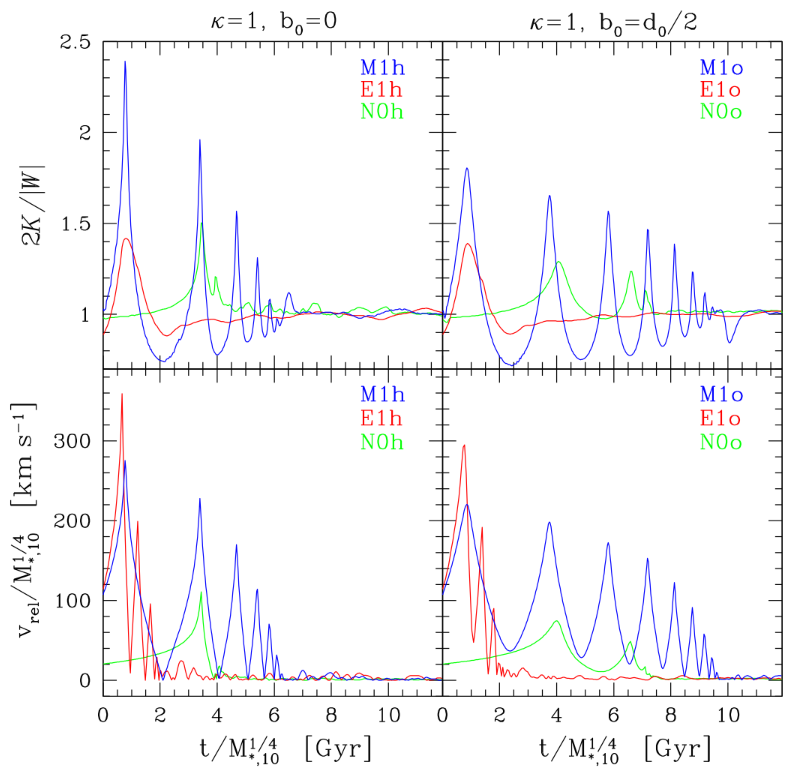
\includegraphics[width=0.5\linewidth]{Nipoti_Londrillo_2007.png}
    \caption{Time evolution of the virial ratio (top panels) and of
the barycentric relative speed (bottom panels) for the two sets of galaxy merger simulations: head-on (left panels) and off-centre (right panels). Blue, red, and green curves refer to MOND, equivalent Newtonian, and purely baryonic Newtonian simulations, respectively. Picture from \textcite{Nipoti_Londrillo_2007}.}
    \label{Virial ratio image}
\end{figure}
Therefore, during the virialization process, both $K$ and $W$ undergo oscillations about their equilibrium values. Consequently, Equation (\ref{virial condition}) is no longer satisfied at every instant; rather, the system obeys the time-dependent virial theorem,
\begin{equation}
\frac{1}{2}\ddot{I}=2K+W,
\label{time_dependent_virial}
\end{equation}
where $I$ denotes the polar moment of inertia. In this regime, $\ddot{I}$ remains small but non-zero, quantifying the departure from virial equilibrium. Owing to Equation (\ref{virial condition}), the mean star undergoes corresponding variations in its kinetic and gravitational potential energies, maintaining the approximate relation
\begin{equation}
\frac{1}{2}m_*v^2 \sim - \frac{1}{4}m_*\psi
\label{mean_star_kinetic_potential_relation}
\end{equation}
By plugging Equation (\ref{mean_star_kinetic_potential_relation}) into Equation (\ref{Stellar energy}), we obtain the following equivalent expression for the violent relaxation time
\begin{equation}
T_r \equiv \frac{3}{4}
\left\langle
\frac{\psi^2}{\dot{\psi}^{\,2}}
\right\rangle^{-1/2}.
\label{violent_relaxation_time_reformulation}
\end{equation}
Since the polar moment of inertia scales with the total mass $M_*$ of the system and the square of its instantaneous characteristic radius $R_*(t)$, it can be written as
\begin{equation}
I(t)=\lambda^2 M_*R_*^2(t)
\label{moment_of_inertia}
\end{equation}
where $\lambda^2$ is a dimensionless structural parameter expected to be of order unity.\\Let the system undergo small radial perturbations about its virial equilibrium configuration. Specifically, we write the instantaneous characteristic radius as
\begin{equation}
 R_*(t)\approx r_v+\delta R_*
\end{equation}
where $r_v$ is the gravitational radius,
\begin{equation}
r_v=-\frac{GM^2}{U},
\label{gravitational radius}
\end{equation}
and $|\delta R_*| \ll r_v$. Linearizing Equation (\ref{virial condition}) with respect to the perturbation then yields the equation of a simple harmonic oscillator,
\begin{equation}
2\lambda^2r_v\ddot{\delta R_*}
-\frac{GM}{r_v^2},\delta R_*,
\end{equation}
with angular frequency
\begin{equation}
\omega=\left(
\frac{GM}{2\lambda^2R_0^3}
\right)^{1/2}
=
\left(
2\pi G\bar{\rho}
\right)^{1/2},
\end{equation}
in which is introduced the galaxy mean density $\bar{\rho}=3M_*/(4\pi r_v^3)$. Yet, as the gravitational potential $\psi \sim 1/r$, it varies on exactly the same timescale as the radius, i.e. $\dot{\psi} \sim \omega \psi$ , leading to
\begin{equation}
T_r\simeq
\frac{3}{4\omega}.
\label{violent_relaxation_time_final}
\end{equation}

EXAMPLE







\section{Two-Body Relaxation and Dynamical Friction}
\label{sec:Two-Body Relaxation and Dynamical Friction}











Let us begin with deriving the two-body relaxitation time, hereafter $t_{2b}$, beyond which gravitational encounters alter stellar trajectories driven by the potential generated by $\rho(r)$, proxy of the real distribution of stars. Thus, systems whose age does not exceed the associated two-body relaxitation time, i.e. $t_{age}<t_{2b}$, will be referred to as collisionless, otherwise  we talk about collisional systems and granularity will be important.\\\textcite{Chandrasekhar_1943} approach  provides an estimate of $t_{2b}$ by considering cumulative orbital deflections under the Impulsive Approximation. It consists of the following two assumptions:
\begin{enumerate}
    \item   All stellar encounters are indipendent of the others. Therefore, multiple interactions are suppressed.
    \item  The gravitational influence of the remaining $N-2$ stars is negletted, resulting in hyperbolic two-body encounters only.
\end{enumerate}
The first tool we need to introduce in order to deal with this treatment, but will be used in the next Sections as well, is the one-particle phase-space distribution function (DF) $f(\mathbf{x_f},\mathbf{v_f},t)$ of the field stars, which depends on the star position $\mathbf{x_f}$, velocity $\mathbf{v_f}$ and time.
provides the probability density of finding a particle at point $((\mathbf{x_f},\mathbf{v_f})$ of the phase-space at time $t$. By definition, the stellar density is thus
\begin{equation}
\rho(\mathbf{x_f},t)=\int_{\mathcal{R}^3}d^3\mathbf{v_f}f(\mathbf{x_f},\mathbf{v_f},t).
\end{equation}
Under the simplifying assumption of a spatially homogeneous distribution and an isotropic velocity field, the degrees of freedom (d.o.f.) are reduced, and the distribution function can be expressed as
\begin{equation}
    f(\mathbf{x_f},\mathbf{v_f})=n_fg(v_f);
\end{equation}
hence, the DF has become the product of the position-indipendent number density and probability density function $g$ in the velocity space\\Two-body encounters between the test particle $m_t$ and the field star $m_f$ will induce change in some orbital property $P$. The cumulative effect of two-body encounters leads to a time variation of $P$, which is quantified by the diffusion coefficient $D(P)$; the Impulsive Approximation enables us ti write it as
\begin{equation}\label{diffusion coeff def}
    D(P)\equiv 2\pi n_f\int_{\mathcal{R}^3} d^3\mathbf{v_f}\|\mathbf{v_t}-\mathbf{v_f}\|g(v_f)\int_0^\infty db\langle P\rangle b,
 \end{equation}
where $\langle P\rangle$ indicates the angle average and $b$ the impact parameter.\\A usefull indicator of changes in the stellar trajectories may be the orbital property $P=\Delta\mathbf{v_{t\perp}}$, that is the component of the test particle velocity variation perpendicular to the initial relative velocity. However, under the assumption of isotropy, the first-order diffusion coefficients in the velocity components vanish \parencite{binney_2011}. Therefore, at higher order, the quantity $P=\|\Delta v_{t\perp} \|^2$ becomes the relevant orbital parameter for determining $t_{2b}$ at leading order. Taking advantage of the Born aproximation of small angle scattering, holding for small deflection angles, 
\begin{equation}
    \|\Delta v_{t\perp} \|\simeq \frac{2Gm_f}{vb}
\end{equation}
and plugging it into Equation (\ref{diffusion coeff def}) returns
\begin{equation}
    D(\|\Delta v_{t\perp} \|^2)\simeq 8\pi G^2m_f^2n_f\int_{\mathcal{R}^3}d^3\mathbf{v_f}\frac{g(v_f)}{v}\int_0^\infty \frac{db}{b}.
\end{equation}
Two logarithmic divergences arise from the integral over $b$: the so-called ultraviolet divergence at $b=0$, due to the Born approximation, and the infrared divergence at $b=+\,\infty$ because of the used model, i.e. an infinite and homogeneus system. Neverthless, Adopting $b_{\pi/2}$ as lower limit and introducing a fiducial upper limit $b_{max}$, that we expect to exist due to the finite size of real stellar systems, it follows
\begin{equation}
D(\|\Delta \mathbf{v}_{t\perp}\|^2) \sim 8\pi G^2 n_f m_f^2 
\int_{\mathbb{R}^3} \frac{g(v_f)\ln \Lambda}{v} \, d^3 \mathbf{v}_f,
\end{equation}
where $\ln{(\Lambda)}=\ln{(b_{max}/b_{\pi/2})}$, is the so called Coulomb logarithm. Although it depends on the velocity field, through the impact parameter $b_{\pi/2}$ corresponding to a deflection angle of $\pi/2$, it can be defined the velocity-weighted Coulomb logarithm $\ln{(\bar{\lambda})}$ so that
\begin{equation}
\int_{\mathbb{R}^3} \frac{g(v_f)\ln \Lambda}{\|\mathbf{v}_t - \mathbf{v}_f\|} \, d^3 \mathbf{v}_f
\equiv \Psi(v_t)\ln \bar{\Lambda},
\end{equation}
with
\begin{equation}\label{Rosenbluth potential}
    \Psi(v_t)=\int_{\mathcal{R}^3}\frac{g(v_f)}{\|\mathbf{v_t}-\mathbf{v_f}\|}d^3\mathbf{v_f},
\end{equation}
being the Rosenbluth potential. One of the greatest semplifications brung by isotropy consist of the possibility to express $\Psi(v_t)$ as
\begin{equation}\label{Rosenbluth potential if isotropy}
\Psi(v_t) = \int_{\mathbb{R}^3} \frac{g(v_f)}{\|\mathbf{v}_t - \mathbf{v}_f\|} \, d^3 \mathbf{v}_f
\equiv \frac{\Xi(v_t)}{v_t} + 4\pi \int_{v_t}^{\infty} g(v_f) v_f \, dv_f,
\end{equation}
where
\begin{equation}
\Xi(v_t) = 4\pi \int_{0}^{v_t} g(v_f) v_f^2 \, dv_f,
\qquad
\Xi(\infty) = 1
\end{equation}
is a normalized function by virtue of the $g(v_f)$ function normalization.\\In the high velocity limit, the monopole term of Equation (\ref{Rosenbluth potential if isotropy}) is the dominant to the leading order and 
\begin{equation}\label{t_2b}
    t_{2b}\equiv\frac{v_t^2(-\infty)}{D(\Delta E_{t\perp})}\sim \frac{v_t^3}{8\pi G^2n_fm_f^2ln\bar\Lambda}.
\end{equation}

On one hand, as just seen, two-body encounters give rise to the heating of the test particle in the direction perpendicular to the initial relative velocity, being deflected; on the other hand the same particle is slowed down by Dynamical friction as result of long range interaction \cite{Baumgardt_2006}.





\begin{equation}\label{velocity first order diffusion coefficient}
    \frac{d\mathbf{v_t}}{dt}=D[\Delta \mathbf{v_t}]=-4\pi G^2 m_t m_f\ln{\Lambda}\int d^3\mathbf{v_f}f(\mathbf{v_f})\frac{\mathbf{v_t}-\mathbf{v_f}}{|\mathbf{v_t}-\mathbf{v_f}|^3}
\end{equation}



\begin{equation}\label{Chandrasekhar dynamical friction equation}
    \frac{d\mathbf{v_t}}{dt}=-16\pi^2 G^2 m_t m_f\ln{\Lambda}\left[\int_{0}^{v_t}dv_f\, v_f^2 f(v_f)\right]\frac{\mathbf{v_t}}{v_t^3}
\end{equation}


\begin{equation}\label{Chandrasekhar dynamical friction equation for MB}
    \frac{d\mathbf{v_t}}{dt}=-4\pi \ln{\Lambda}\left[erf(X)-\frac{2X}{\sqrt{\pi}}e^{-X^2}\right]\frac{G^2m_t\rho(r)}{v_c^3}\mathbf{v_t}
\end{equation}


where 
\begin{equation}\label{error function}
    erf(X)=\frac{2}{\sqrt{pi}}\int_{0}^{X}dt \, e^{-t^2}
\end{equation}



\begin{equation}\label{dynamical friction angular momentum loss eq}
    \frac{d\tilde{L}}{dt}=\tilde{F}r
\end{equation}

with 

\begin{equation}\label{dynamical friction angular momentum and force}
    \tilde{L}=m_t\sqrt{Gm_fr}        \qquad  \tilde{F}=-C(\Lambda,X)\frac{G^2m_t^2\rho(r)}{v_c^2}
\end{equation}

with $C(\Lambda,X)$ implicitly defined by Equation (\ref{dynamical friction angular momentum and force})
and $X\equiv v_c/\sigma\sqrt{2}$

\begin{equation}\label{r(t) diff. eq. for dynamical friction}
    r^{-5/2}\frac{dr}{dt}=-C(\Lambda,X(r))\frac{G^2m_t^2}{m_f^{3/2}}\rho(r)
\end{equation}




\begin{equation}\label{SIS matched with stellar cusp}
\rho(r) =
\begin{cases}
\rho_{\mathrm{inf}}\left(\dfrac{r}{r_{\mathrm{inf}}}\right)^{-\gamma}
& \text{if } r < r_{\mathrm{inf}} \\[6pt]
\dfrac{\sigma^2}{2\pi G r^2}
& \text{if } r > r_{\mathrm{inf}}
\end{cases}
\end{equation}



\begin{equation}\label{Power low distribution}
    \rho(r)=\rho_0\left(\frac{r}{r_0}\right)^\gamma
\end{equation}





If $M_*(r<a_0)=2M_2$ then 

\begin{equation}\label{a_0 of stellar cusp model}
a_0 = (3 - \gamma)\,\frac{G M}{\sigma^2}
\left(\frac{q}{1 + q}\right)^{\frac{1}{3 - \gamma}}
= r_{\mathrm{inf}}
\left(\frac{q}{1 + q}\right)^{\frac{1}{3 - \gamma}}
\end{equation}


\begin{equation}\label{X of the stellar cusp}
    \sigma^2(r)=\frac{v_c^2(r)}{2(\gamma-1)} \quad \Rightarrow \quad X=\sqrt{\gamma-1}
\end{equation}

Integrating from $r_{0}$ to $r(t)$ leads to

\begin{equation}\label{r(t) of stellar cusp under dynamical friction}
r(t)=
\begin{cases}
\left[r_0^{\gamma-3/2}-C(\Lambda,X)\frac{\sqrt{G}m_t}{m_f^{3/2}}\left(\gamma-\frac{3}{2}\right)\rho_0r_0^{\gamma}t\right]^{\frac{1}{\gamma-3/2}}
& \text{if } \gamma \ne \frac{3}{2} \\[6pt]
r_0\exp\left[-C(\Lambda,X)\frac{\sqrt{G}m_t}{m_f^{3/2}}\rho_0r_0^{3/2}t\right]
& \text{if } \gamma = \frac{3}{2}
\end{cases}
\end{equation}


If we define $t_{fric}$ such that $r(t_{fric})=a_0$ we get


\begin{equation}\label{t_fric of stellar cusp}
t_{fric}=
\begin{cases}
\frac{m_f^{3/2}(r_{inf}^{\gamma-3/2}-a_0^{\gamma-3/2})}{C(\Lambda,X)\sqrt{G}m_t\left(\gamma-\frac{3}{2}\right)\rho_{inf}r_{inf}^{\gamma}(\gamma-3/2)}
& \text{if } \gamma \ne \frac{3}{2} \\[6pt]
\frac{m_f^{3/2}}{C(\Lambda,X)\sqrt{G}m_t\rho_0r_0^{3/2}}  \ln{\left(\frac{r_{inf}}{a_0}\right)}
& \text{if } \gamma = \frac{3}{2}
\end{cases}
\end{equation}


Being intrinsically inelastic,, give rise to mergers, hosting an MBH binary (see e.g. \textcite{Baumgardt_2006}).



\section{Black Hole Binary–Star Three-Body Scattering}\label{sec:Gravitational Slingshot Effect}
When operating during major merger events, the dynamical friction brings both MBHs towards the galactic center of the merger remnant, reducing their separation and eventually causing the BHs to cross other sphere of influence. At the end of this process, beyond which three-body stellar encounters take over the long-range intercations with field stars, they find themselves tied together due to their mutual gravitational attraction and at a relative distance of the order of $a_0$, defined as the binary separation at which the enclosed stellar mass is equal to the secondary BH mass $M_2$  \parencite{Baumgardt_2006}. Therefore, in this section we report the main theoretical aspects of three-body encounters, as they represent the dominant process promoting the shrinking of the binary and prepare the conditions for the subsequent inspiral phase.\\Each time a low angular momentum star, hereafter "loss-cone" star, passes close to the BH binary, an exchange of energy and angular momentum between three bodies takes place. Under suitable conditions, the incoming star is ejected at a higher velocity, carrying away the excess energy extracted from the BH pair and thus promoting its progressive hardening. This process is known as  "Slingshot effect" \parencite{Mikkola_1992}.\\Let us focus on the so-called "two-body problem" and some the related results as they will be usefull in dealing with the physics of the stellar slingshot. Given the test and field particles, of masses $m_t$ and $m_f$ respectively and reduced mass $\mu$, the system total energy in the mass center frame $S_{CM}$ turns out to be
\begin{equation}
\label{E_in_S_cm}
    E=\frac{1}{2}\mu\|\mathbf{v}\|^2-\frac{Gm_fm_t}{r},
\end{equation}
 where  $r(t)\equiv \|\mathbf{x_t}-\mathbf{x_f}\|$ and $\mathbf{v}(t)\equiv \mathbf{v_t}-\mathbf{v_f}$ denote particles relative separation and velocity.\\For two unbound particles, moving along hyperbolic orbits in $S_{CM}$, the energy conservation imposed by Equation (\ref{E_in_S_cm}) at two infinity configuarations $r(-\infty)=r(+\infty)=+\infty$ returns
\begin{equation}\label{relative velocity modulus conservation}
     \|\mathbf{v}(-\infty)\|=  \|\mathbf{v}(+\infty)\|.
\end{equation}
According to Equation (\ref{relative velocity modulus conservation}), the magnitude of the test particle velocity is conserved in the inertial frame centered on
the field particle. Therefore, the encounter results only in a rotation of the velocity vector $\mathbf{v}$ and the corresponding velocity change $\Delta\mathbf{v}=\mathbf{v}(+\infty)-\mathbf{v}(-\infty)$ can be conveniently decomposed  as the sum of the components perpendicular and parallel to the initial relative velocity $\mathbf{v}(-\infty)$ as follows
\begin{equation}
    \mathbf{v}(+\infty)=\mathbf{v}(-\infty)+\Delta\mathbf{v}_\parallel +\Delta\mathbf{v}_\perp.
\end{equation}
Plugging this expression for $\mathbf{v}(+\infty)$ into Equation (\ref{relative velocity modulus conservation}) allows us to obtain the identity
\begin{equation}\label{slingshot negative scalr product}
     \| \Delta\mathbf{v}_\parallel\|^2+  \| \Delta\mathbf{v}_\perp\|^2+\langle \Delta\mathbf{v}_\parallel, \mathbf{v}(-\infty) \rangle=0.
\end{equation}
A first glance at this formula reveals that a necessary condition for it to hold is that the scalar product must be a negative term. This observation will be crucial in assessing whether binary BH-star interaction leads to the shrinking or the softening.\\The just derived results correspond to a constraint on particles relative velocity valid in a specific inertial frame. However, one is free to describe the interaction in an arbitrary inertial frame $S_0$, where both bodies may be seen moving; hence, a generalization is required.\\In $S_0$ the close encounter causes both $E_t$ and $E_f$ to change, preserving at each time the validity of energy conservation equation of the system. Between the two configurations at infinite relative separation, the test particle experience a net variation of mechanical energy
\begin{equation}\label{t energy variation 1}
    \Delta E_t=\frac{1}{2}m_t[\|\mathbf{v_t}(+\infty)\|^2-  \|\mathbf{v_t}(-\infty)\|^2]=-\Delta E_f,
\end{equation}
which is perfectely compensated by the variation of the field particle mechanical energy, that is
\begin{equation}
 \Delta E= \Delta E_t+\Delta E_f=0.
\end{equation}
By combinig the velocity composition law
\begin{equation}
    \mathbf{v_t}(t)=\mathbf{v_{CM}}+\frac{\mu}{m_t}\mathbf{v}(t)
\end{equation}
and the conservation of the mass center velocity vector $\mathbf{v_{CM}}$, valid for isolated systems, Equation (\ref{t energy variation 1}) takes the form \parencite{Ciotti_2021}
\begin{equation}
    \Delta E_t=\mu\langle \Delta\mathbf{v}, \mathbf{v_{CM}} \rangle.
\end{equation}
We are now in a position to address three-body scattering involving a gravitationally bound BH binary and an incoming star. The dynamics of this encounter can be understood by considering the limiting case of strongly asymmetric binary in which $M_1\gg M_2\gg m_*$ so that both the star and the secondary BH, having masses $m_*$ and $M_2$, can travel along nearly Keplerian orbits around $M_1$ with slightly different radii and, consequently, possess slightly different Keplerian velocities. The secondary BH acts as the field particle, while the star plays the role of the test particle. The primary BH serves only to establish the relative velocity between the two bodies. As a result, the center of mass motion of this gravitationally unbound pair is essentially determined by the orbit of $M_2$ around $M_1$. Therefore, the approximation
\begin{equation}\label{Primary BH approx CM}
    \mathbf{x_{CM}}\simeq \mathbf{x_f}, \qquad\mathbf{v_{CM}}\simeq \mathbf{v_f},
\end{equation}
applies and the mass center will move locally at costant velocity if the observation time is short compared to the orbital period, thus making negligible its acceleration.\\Hereafter, by analogy with the previous notation, we identify $M_2\equiv m_f$ and $m_*\equiv m_t$.

\paragraph{Binary hardening.}
When the star is place outside the secondary BH orbit, the Keplerian velocity profile imposes $\|\mathbf{v_f}(-\infty) \| =\| \mathbf{v_{CM}}\| > \|\mathbf{v_t}(-\infty) \|$. Therefore, at point where $m_f$ surpasses $m_t$ and they are both located on the same radius, $\mathbf{v}(-\infty)$ is nearly antiparallel to $\mathbf{v_{CM}}$ and $\Delta\mathbf{v}_\parallel$ can be read as the projected vector along $\mathbf{v_{CM}}$ rather than $\mathbf{v}(-\infty)$. Taking advantage of Equation (\ref{slingshot negative scalr product}), it follows that
\begin{equation}
\label{stellar_hardening_inequality}
    0<\langle \Delta\mathbf{v}_\parallel, \mathbf{v_{CM}} \rangle=\langle \Delta\mathbf{v}, \mathbf{v_{CM}}\rangle=\Delta E_t/\mu.
\end{equation}
Equation (\ref{stellar_hardening_inequality}) shows that in the reference system centered on $M_1$ the star gains orbital energy and is scattered onto a wider orbit. On the other hand, the secondary BH experiences an equal and opposite change in orbital energy, leading to a reduction of the binary separation and, consequently, to binary hardening.\\ It is worth of noticing that if $\Delta E_t>|E_t(-\infty)|$, which occurs at very high circular velocity of the binary BHs, stellar ejection occurs; in this regime ‘‘hypervelocity stars’’ (HVSs) travelling along nearly radial orbits are produced \parencite{Sesana_2006}.

\paragraph{Binary softening.}
Contrary to the previous case, binary softening takes place when the star is place inside the secondary BH orbit. Now $\mathbf{v}(-\infty)$ is nearly parallel to $\mathbf{v_{CM}}$ at the crossover point and by repeating the same arguments used above it is found
\begin{equation}
     E_t/\mu=\langle \Delta\mathbf{v}, \mathbf{v_{CM}}\rangle=\langle \Delta\mathbf{v}_\parallel, \mathbf{v_{CM}} \rangle<0.
\end{equation}
On one hand the star loses energy to the binary, it is pushed inward and may undergo tidal disruption due to primary BH \parencite{Lightman_1977}; on the other hand the binary gains energy and its semimajor axis increases, resulting in binary softening.

\par\vspace{0.5cm}
\noindent
Although our discussion has so far focused on a specific three-body scattering configuration, the results can be readily generalized by observing that the distinction between binary hardening and softening is determined by the relative magnitude of the BH binary's orbital velocity  and the velocity of the incoming loss-cone star.\\The binary BH embidded in an isotropic stellar background with costant velocity dispersion $\sigma$ is expected to undergo three-body scatterings with loss-cone stars that will approach the galactic centre where the binary lives with velocity of the order of $\sigma$. Because the specific binding energy of a keplerian with total mass $M=M_1+M_2$, reduced mass $\mu$ and semimajor axis $a$ is
\begin{equation}
 E_b=\frac{G\mu}{2a}
\end{equation}
and the specific energy of the loss-cone star is of the order of $\sigma^2$, the velocity criterion can be conveniently reformulated in terms of the specific energy. When $E_b\ll \sigma^2$, the binary is said to be soft, and repeated stellar encounters tend to further decrease its binding energy. Conversely, when $E_b\gg \sigma^2$, the binary is hard, and stellar encounters, on average, increase its binding energy. This behavior is well summarized by Heggie's law \parencite{Heggie_1975}.
\medskip

\noindent\textbf{Heggie's law. --}
\emph{On average, hard binaries get harder and soft binaries get
softer.}
\medskip

\noindent By extrapolation of the two limiting cases, one can define the "hardening radius" $a_h$ as the binary separation at which binary passes from the soft to the hard regime. Despite its expected weak dependence on the BH mass ratio, throughout this work we adopt the definition proposed by \textcite{Quinlan_1996}, unless otherwise specified:\begin{equation}\label{a_h definition}
 a_h=\frac{GM_2}{4\sigma^2}.
\end{equation}
At this stage, it should be clear that stellar scattering plays a fundamental role in driving the binary toward the regime in which GWs emission dominates its evolution. Nevertheless, one may wonder how a binary can evolve from the soft to the hard regime. The key point is that most of the work for this evolution to continue in the the direction of binary hardening is done by dynamical friction with the stellar background rather than individual encounters, as explained in Section \ref{sec:Two-Body Relaxation and Dynamical Friction}.



















\section{Stellar Scattering and Loss Cone Problem}\label{sec:Loss Cone}
\cite{Lightman_1977}Let us consider a massive object $M$- it may be a BH binary- residing at center of a stellar distribution; far enough from it, stars are unbound, move with rms velocity $\langle v^2\rangle^{1/2}$ and obey to the Maxwellian distribution, i.e. velocity field is isotropic.\\Combining $M$ and the rms velocity, we define the influence radius, beyond which stars are mainly unbound, $r_a\sim 2GM/\langle v^2\rangle$. Stellar orbits are assumed to be driven by the gravity of $M$ at $r<r_a$.\\Moreover, close encounters between stars and $M$ may lead to stellar consumption via several processes; they occur on a time scale of the order of the dynamical one, i.e. one orbital period, if $r$ is smaller than the tidal radius $r_t$, where
\begin{equation}
    t_d=P(E)=\frac{2\pi GM}{(2|E|)^{3/2}}.
\end{equation}

A steady state solution in the range $r_t<r<r_a$ requires the rate of stars diffusing inward, crossing $r_a$, over $t_{2b}$, equal to the rate of stars consumed at $r_t$, behaving as a sink of this problem. \\If $E$ and $J$ denote respectively the star specific energy and angular momentum, it is worth of noticing  that  not only stars with low energy, i.e. $E\approx E_t\equiv -GM/r_t$ are removed but also high $E$ low $J$ might experience the same fate. At pericenter the radial velocity vanishes and 
\begin{equation}
    E=\frac{J^2}{2r^2}-\frac{GM}{r};
\end{equation}
hence a star can find itself inside $r_t$ if 
\begin{equation}\label{loss cone definition}
    J\le J_{min}\equiv \left[2\left(E+\frac{GM}{r_t}\right)\right]^{1/2}r_t.
\end{equation}
Inequality (\ref{loss cone definition}) defines the so called "Loss Cone".

\subsection{Bound stars consumption}
\subsubsection{One-Dimensional Analysis }
As stellar orbit shape and size around $M$ are set by $E$ and $J$, the one particle DF can be written as $f=f(E,J)$ according to Jean's theorem. Therefore, the nature of the problem is 2-dmensional; neverthless, by negletting loss cone effects, an approximated one-dimensional solution can be obtained under the assumption of quasi-circular orbits where $J=J_{max}(E)=GM/\sqrt{2|E|}$.\\In this scenario the boundary conditions for bound stars at $r_t<r<r_a$ read $E_t<E<E_a$ and the DF is $f=f(E)$. The steady stae self-similar solution obtained by Peebles relies on the power law DF $f(E)=k|E|^p$ and the corresponding maximum flux of stars in the $E$ space is $F_{max}\sim N(<r)/t_{2b}(r)$.\\By definition \begin{equation}
    N(<r)=\int f(E)d^3\mathbf{v}\sim |E|^{p-3/2}
\end{equation}
and $t_{2b}\sim v^3/n\sim |E|^{-p}$; they combine into
\begin{equation}
    F_{max}(E)\sim |E|^{2p-3/2}.
\end{equation}
A more accurate analysis yields
\begin{equation}
    F(E)=-F_{max}(E)\beta(p),
\end{equation}
where the the exact solution, that is the value of $p$, can be derived by imposing $F(E)=const$ from the stationarity condition.\\Bahcall and Wolf (1976) found the solution $p=1/4$.
\subsubsection{Two-dimensional Analysis: Loss Cone effects}

Let us focus on loss cone effects; the DF is now in general a function of both $E$ and $J$.\\By assuming stellar encounters to be dominated by distant and weak gravitational interactions, $J$ diffusion problem can be treated with RW theory and it can be defined the angular momentum step size
\begin{equation}\label{j_2 definition}
    j_2\sim J_{max}(t_d/t_r)^{1/2},
\end{equation}

it represents the dispersion in $J$ suffered over $t_d$.\\The dimensionless quantity
\begin{equation}
    q(E)\equiv\frac{j_2^2}{J_{min}^2}
\end{equation}
enables us to distinguish two extreme scenarios in terms of stellar consumption rate:
\begin{itemize}
  \item  \(q \ll 1\) (Empty Loss Cone): $j_2\ll J_{min}$ implies a too small RW step size for diffusion to be effective and only stars with $J$ close to $J_{min}$ can enter the loss cone.\\Since $t_{2b}\gg t_d$ the loss cone remeins nearly empty and the capture rate is limited by diffusion.
  \item  \(q \gg 1\) (Full Loss Cone): $j_2\gg J_{min}$ implies a large RW step size compared to loss cone size and many stars in the range $J_{min}<J<J_{min}+j_2$ can be captured.\\In this regime equation (\ref{j_2 definition}) predicts many weak stellar encounters per orbital period and thus an almost full loss cone as the star consumption, takes place over $t_d$,is slower than stellar capture rate; stellar consumption rate is limited by orbital period.
\end{itemize}

The stellar consumption rate per unit energy is
\begin{equation}  
-F_E(E) \sim
\begin{cases}
\frac{F_{max}(E)|E|^{-1}}{ln\left(\frac{GM}{|E|r_t}\right)}, & q \ll 1 \\
q^{-1}F_{max}(E)|E|^{-1},   & q \gg 1
\end{cases}
\end{equation}
and is strongly peaked at $E_{crit}$- or equivalently at $r_t$- at which $q(E_{crit})\approx1$.

\subsection{Unbound stars consumption}
Previously it has been pointed out that the majority of the stellar capture involves stars at $E_{cri}$ (or $r_{crit}$), this indicates that if the critical radius exceeds the influence radius, within which stars are mainly bound, this process affects primarly Unbound stars.\\In this region the stellar flux becomes
\begin{equation}
    F_{max}\sim \frac{N(<r)}{t_{2b}(r)}\sim \left(\frac{r}{r_a}\right)^3 F_{max}(E_a)
\end{equation}



Several times beyond $t_{2b}$ the system enters the collisional regime and first order
corrections to the CBE are needed; the Fokker-Planck equation is an example of this:
\begin{equation}
    \frac{Df}{Dt}=C[f]
\end{equation}
where simplifications on the collision operator $C[f]$ can be done.\\In this scenario $f$ is
no longer conserved along the orbit of the potential $\Phi$ and diffusion in the PS occurs,
both $E$ and $L$ of a single star can change due to collisions, at odds with the CBE regime
where, for istance $DH/Dt=0$. It is used in the loss cone problem.






\subsection{Loss cone theory role in Hybrid Model}
Devoted to determine evolutionary tracks for BH binaries evolving via three-body scattering with background stars and GWs emission \cite{Quinlan_1996} \cite{Sesana_2010}, one of the key points of the adopted model turns out to be the nature of stars involved in close encounters with the binary. At beginning, when the pair forms, all stars intersecting its orbit, i.e. populating the "Loss cone" are expelled via gravitational slingshot effect mainly; this mechanism results in the erosion of the stellar core and drives efficiently the binary down to a separation of the order of the hardening radius. Thereafter, for the shrinking to proceed, loss cone orbits must be refilled. Without addressing the problem concerning how this process takes place, it is relevant to point out that, once depleted all the stars inside $a_h$, stars candidate to replenish the loss cone come from outside this region.\\Therefore, for nearly equal mass BHs, having $a_h\sim r_{inf}$, or shallow stellar cores from the transistion soft/hard on, the scattering with unbound stars becomes dominant until the binary develops efficient GWs emission phase.\\Once established whether the vast majority of stars exchanging energy and angular momentum with the binary are bound or unbound to such a pair, the Hybrid model should take into account loss cone status through some parameters. This information enters the model by means of the normalizing density and velocity dispersion of $H_u$ and $K_u$; when they are set equal to their value at $r_{inf}$, the model is assuming that the loss cone is always full at $r>r_{inf}$ (pinhole regime) and empty at $r<r_{inf}$ (diffusive regime).\\Testing the model by changing the normalizing quantities  serves to investigate how the loss cone refilling affects the binary evolution.



\begin{figure}
    \centering
    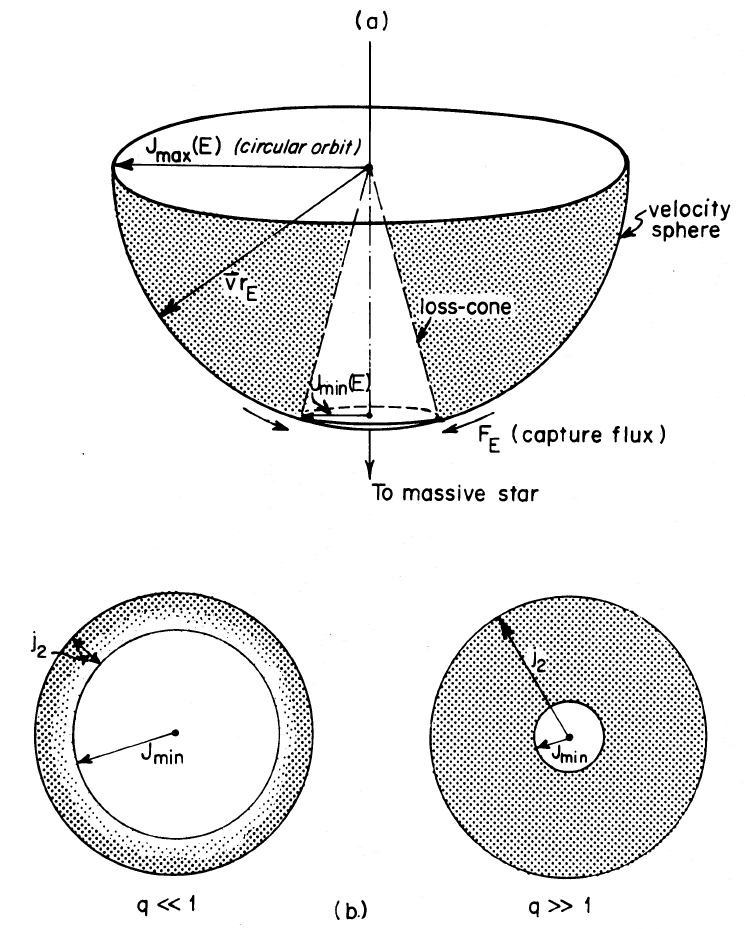
\includegraphics[width=0.5\linewidth]{Loss_cone.png}
    \caption{Fig. 1(a).—Velocity distribution of stars with fixed energy $E$;$J$ varies accordingly to the direction of $\mathbf{v}$ emphasising the two-dimensional nature of the problem. The vertical axis points towards the compact object of mass $M$.
Fig. 1(6).—The velocity sphere viewed from below. On the left the empty loss cone scenario; stellar density is nearly indipendent of $J$ everywhere but $J\gtrsim J_{min}$ where is quickly declines. On the right the full loss cone regime; consumed stars are immediately replenished by stars from a region much more extended- and uniform density- than the loss cone itself (the “pinhole” limit).}
    \label{loss cone image}
\end{figure}









\section{Gravitational Radiation from Black Hole Binaries}





\subsection{Linearized Gravitational Field Equation}

The starting point of the theoretical derivation of GWs properties, such as the energy and angular momentum they transport, from BH binary and the associated back-reaction on the astrophysical source, is the linearization of  field equations of Generl Relativity (GR)
\begin{equation}\label{Einstein field eq.}
    R_{\mu \nu}-\frac{1}{2}g_{\mu \nu} R=\frac{8\pi G}{c^4}T_{\mu \nu}.
\end{equation}
These constitute ten coupled, non-linear, second-order partial differential equations for the metric tensor; neverthless, they are not sufficient to uniquely set the ten indipendent components of $g_{\mu\nu}$ due to the four  Bianchi identities, equivalent to the same number of differential constraints, resulting in six  independent equations only. These four degrees of freedom are intimately connected to gauge symmetries, reflecting the arbitrariness of the four coordinates $x^\mu$ used to represent and solve Equation (\ref{Einstein field eq.}).\\To show how gravitational radiation emerges from Equation (\ref{Einstein field eq.}), we need to expand it around the Minkowski metric $\eta_{\mu \nu}=diag(-1,+1,+1,+1)$; therefore we assume
\begin{equation}
    g_{\mu \nu}(x)=\eta_{\mu \nu}+h_{\mu \nu}(x),
\end{equation}
with $|h_{\mu \nu}|\ll1$ being a symmetric tensor representing a small perturbation of the flat spacetime.\\The left-hand side of Equation (\ref{Einstein field eq.}) encodes the geometry and curvature of spacetime and contains all terms that are functions of the metric; in terms of the affine connection
\begin{equation}\label{affine connection def}
    \Gamma^\lambda _{\mu\nu}=\frac{1}{2}g^{\lambda \rho}(\partial_\mu g_{\nu\rho}+\partial_\nu g_{\rho\mu}-\partial_\rho g_{\mu\nu})
\end{equation}
and the Riemann tensor
\begin{equation}\label{Riemmann tensor def}
    R_{\lambda\mu}{}^{\rho}{}_{\nu}=\partial_\lambda \Gamma_{\mu\nu}^\rho-\partial_\mu \Gamma_{\lambda\nu}^\rho+\Gamma_{\lambda\sigma}^\rho \Gamma_{\mu\nu}^\sigma-\Gamma_{\mu\sigma}^\rho \Gamma_{\lambda\nu}^\sigma,
\end{equation}
they can be expressed indeed as 
\begin{equation}\label{Ricci tensor def}
    R_{\mu\nu}=R_{\sigma\mu}{}^{\sigma}{}_{\nu}
\end{equation}
and 
\begin{equation}\label{Ricci scalar def} R=g^{\alpha\beta}R_{\alpha\beta}=R_\sigma^\sigma.
\end{equation}
On the right-hand side, instead, appears the Energy-Momentum tensor; it can be read as the source term of the gravitational field equations and turns out to be
\begin{equation}\label{Energy-Momentum tensor def}
    T^{\mu\nu}=(\rho+p/c^2)u^\mu u^\nu+pg^{\mu\nu}
\end{equation}
for a perfect fluid of density $\rho$, pressure $p$ and four-velocity $v^\mu$.\\It straightforward to prove that, to the first order in the metric perturbation, they become:
\begin{equation}\label{linearized Ricci tensor}
    R_{\mu \nu}=-\frac{1}{2}(\Box h_{\mu \nu}+\partial_\mu \partial_\nu h-\partial_\lambda\partial_\mu h_\nu^\lambda-\partial_\nu\partial_\lambda h_\mu^\lambda)
\end{equation}
 and
\begin{equation}\label{linearized ricci scalar}
    R=\partial_\mu \partial_\nu h^{\mu\nu}-\Box h,
\end{equation}
where $h$ denotes $h_{\mu \nu}$ trace.\\Defining the so-called "trace reverse" of $h_{\mu\nu}$
\begin{equation}\label{trace reverse definition}
    \bar{h}_{\mu\nu}\equiv h_{\mu\nu}-\frac{1}{2}\eta_{\mu\nu} h
\end{equation}
and plugging the terms of Equations (\ref{linearized Ricci tensor}) and (\ref{linearized ricci scalar}) into Equation (\ref{Einstein field eq.}), the field equations take the form
\begin{equation}\label{linearized Einstein Eq. LONG}
    \Box \bar{h}_{\mu\nu} + \eta_{\mu\nu}\partial_\alpha\partial_\beta \bar{h}^{\alpha\beta}-\partial_\mu\partial_\lambda \bar{h}^\lambda_\nu-\partial_\nu\partial_\lambda \bar{h}^\lambda_\mu=-\frac{16\pi G}{c^4}T_{\mu\nu}.
\end{equation}
Taking advantage of the gauge freedom of Equation (\ref{Einstein field eq.}), it can be performed an infintesimal coordinate transformation of the kind
\begin{equation}
    x^\mu \rightarrow{}x'^\mu=x^\mu+\xi^\mu(x);
\end{equation}
as tensors obey to precise law of transformation, this yields
\begin{equation}
    \bar{h}'_{\mu\nu}=\frac{\partial x^\alpha}{\partial x'^\mu}\frac{\partial x^\beta}{\partial x'^\nu}\bar{h}_{\alpha\beta}\approx \bar{h}_{\mu\nu}-\partial _\mu \xi_\nu -\partial_\nu \xi_\mu+\eta_{\mu\nu}\partial_\sigma\xi^\sigma.
\end{equation}
Yet, if the four functions $\xi^\mu$ are chosen so as to satisfy the so-called De Donder gauge condition, i.e. $\Box\xi^\mu=\partial_\sigma\bar{h}^{\sigma\mu}$, then $\partial_\sigma\bar{h}'^{\sigma\mu}=0$ and, dropping the prime, Equation (\ref{linearized Einstein Eq. LONG}) semplifies to
\begin{equation}\label{linearized Einstein eq + gauge condition}
\begin{cases}
\Box \bar{h}_{\mu\nu} = -\dfrac{16\pi G}{c^4} T_{\mu\nu} \\
\partial_\mu\bar{h}^{\mu\nu}=0.
\end{cases}
\end{equation}
We are now ready to address the problem of determining  the general solution of the linearized Einstein's equations coupled with the De Donder gauge condition. 


\subsection{Generation and Propagation of Gravitational Waves}

To study the formation of GWs we initially focus on the solution of the problem defined in Equation (\ref{linearized Einstein eq + gauge condition}) inside the source where $T_{\mu\nu}\ne 0$.\\Linear partial differential equations solution can be obtained by the method of Green's function; by definition, the Green's function $G$ is the solution of the associated equation in case of a pont-like source, i.e.
\begin{equation}\label{Green equation}
    \Box_x G(x-x') = \delta^{(4)}(x-x'),
\end{equation}
with $\delta^{(4)}(x-x')$ being the four-dimensional Dirac function.\\It is relevant to note that, apart from the B.C. of the problem, $G$ depends only on the linear operator; therefore, from the radiation problem in electromagnetism, we already know that the proper solution is the retarded Green's function 
\begin{equation}\label{retarded Green function}
    G(x-x')=-\frac{1}{4\pi |\mathbf{x}-\mathbf{x'}|}\delta^{(4)}(ct_{ret}-ct'),
\end{equation}
where 
\begin{equation}\label{retarded time def}
    t_{ret}=t-\frac{|\mathbf{x}-\mathbf{x'}|}{c}
\end{equation}
is the time in past at which the radiation was emitted at $\mathbf{x'}$ in order to be observed at $\mathbf{x}$ at time $t$. Once the Green's function is found, the general solution will be the convolution between it and source term:
\begin{equation}\label{h_mn general solution}
    \bar{h}_{\mu\nu}(t,\mathbf{x})=\frac{4G}{c^4}\int d^3x'\frac{T_{\mu\nu}(t_{ret},\mathbf{x'})}{|\mathbf{x}-\mathbf{x'}|}.
\end{equation}
Prior to examining the formula reported in Equation (\ref{h_mn general solution}) and assessing which additional simplifications can be implemented and when they apply, it is appropriate to analyze how GWs propagate in vacuo.\\Outside the GWs source, $T_{\mu\nu}$ vanishes and, owing to the linearity of the d’Alembert operator, the solution can be expressed as superposition of plane waves without loss of generality, that is
\begin{equation}
    \bar{h}_{\mu\nu}(x)=\int d^3k (A_{\mu\nu}(\mathbf{k})e^{ik_\rho x^\rho}+c.c.)
\end{equation}
However, not all plane waves satisfy the linearized field equation in vacuo along with the gauge condition but linearity enables us to study the properties of a single plane wave separately; consequently, inserting the Ansatz $\bar{h}_{\mu\nu}\sim A_{\mu\nu}e^{ik_\rho x^\rho}$ yields the following two constraints:
\begin{enumerate}
    \item $(k_\rho k^\rho=0)$: the four-vector $k^\mu=(\omega/c,\mathbf{k})$ is a light-like vector (GWs travel at light speed $c$ in vacuo).
    \item $(k_\mu A^{\mu\nu}=0)$: it implies $A^{0\nu}=A^{3\nu}$ if we deal with GWs propagating along the $x^3$ direction, hence $k^\mu=(k,0,0,k)$.
\end{enumerate}
At this stage, the amplitude tensor $A^{\mu\nu}$ possesses six indipendet components --- ten, due to symmetry, reduced by the four constraints imposed by the gauge conditions --- and can be written as
\begin{equation}\label{A^mn 6 dof}   
A^{\mu\nu} =
\begin{pmatrix}
A^{00} & A^{10} & A^{20} & A^{00} \\
A^{10} & A^{11} & A^{12} & A^{10} \\
A^{20} & A^{12} & A^{22} & A^{20} \\
A^{00} & A^{10} & A^{20} & A^{00}
\end{pmatrix}.
\end{equation}
Out of the six polarizations shown in Equation (\ref{A^mn 6 dof}), four are unphysical because they vanish when the residual gauge freedom associated with four arbitrary harmonic functions $\xi^\mu$ is exploited. One is free to adopt functions proportional to the plane wave solutions of the vacuo problem, i.e. $\xi^\mu=\epsilon^\mu e^{ik_\rho x^\rho}$ are harmonic, and to set their amplitudes $\epsilon^\mu$ such that 
\begin{equation}\label{A^mn TT gauge}   
A^{\mu\nu}_{TT} =
\begin{pmatrix}
0 & 0 & 0 & 0 \\
0 & h_+ & h_x & 0 \\
0 & h_x & -h_+ & 0 \\
0 & 0 & 0 & 0
\end{pmatrix}.
\end{equation}
The coordinate system where $A^{\mu\nu}$ is in the form of Equation (\ref{A^mn TT gauge}), with two indipendent polarizations only, and defined by 
\begin{equation}
    \partial_\mu h^{\mu\nu}=0, \quad h^{0\mu}=0, \quad h^i_i=0,
\end{equation}
is referred to as "TT gauge"\footnote{In the TT gauge, according to the definition provided, $\bar{h}_{ij}^{TT}=h_{ij}^{TT}$.}.\\Having analyzed the propagation of GWs in vacuo and the properties of the TT gauge, we are now in the position to focus again on the source solution reported in Equation (\ref{h_mn general solution}). One of the greatest simplifications to this integral consists of the so-called "Compact-source approximation"; it applies outside the source whenever its size is negligible with respect to the source-detector separation. In this regime, we can retain the leading term of the multipole expansion only, thus
\begin{equation}\label{h_mn compact source solution}
    h_{ij}^{TT}(t,\mathbf{x})=\frac{4G}{c^4r}\int d^3x'T_{ij}(t_{ret},\mathbf{x'}).
\end{equation}
Furthermore, far from the source, the conservation of the Energy-Momentum tensor, namely $\nabla_\mu T^{\mu\nu}\approx\partial_\mu T^{\mu\nu}=0$, yields
\begin{equation}\label{h_mn final form}
    h_{ij}^{TT}(t,\boldsymbol{x})=\frac{2G}{rc^4}\ddot{Q}^{TT}_{ij}(t-r/c)
\end{equation}
at lowest order in the low-velocity expansion.\\The term $Q^{TT}_{ij}$ introduced in Equation (\ref{h_mn final form})\footnote{The components with at least one time index are excluded from our analysis because they are constant and therefore do not contribute to GWs formation.} is the representation of the quadrupole moment in the class of coordinate systems satisfying the TT gauge conditions; defining the quadrupole moment of $T^{00}/c^2=\rho$ as
\begin{equation}\label{M_ij definition}
    M^{ij}\equiv \frac{1}{c^2}\int d^3x T^{00}(t,\boldsymbol{x})x^ix^j,
\end{equation}
it is thus possible to write
\begin{equation}\label{Q_ij def}
    Q^{ij}\equiv M^{ij}-\frac{1}{3}\delta^{ij}M_{kk}=\int d^3x\rho(t,\mathbf{x})\left(x^ix^j-\frac{1}{3}r^2\delta^{ij}\right).
\end{equation}
Equation (\ref{h_mn compact source solution}) shows that, unlike electromagnetic radiation, at lowest order the gravitational radiation arises from changes in the quadrupole moment; other important observables such as the energy and angular momentum carried by GWs, needed to estimate the back-reaction, will be derived from the quantities defined in Equation (\ref{Q_ij def}) indeed.\\The energy and angular momentum conservation laws impose that the rates a which these quantities are carried away by GWs at time $t$ and at large separation $r$ from the source coincide with the corresponding rates of orbital energy ---if the emitting system consists of a BH binary--- and angular momentum, negletting the spin contribute, loss evaluated at the appropriate retarded time; in formulae:
\begin{equation}\label{energy loss rate by GWs}
    P_{quad}=\frac{dE_{gw}}{dt}=\frac{G}{5c^5}\langle\dddot{Q}_{ij}\dddot{Q}_{ij}\rangle=-\frac{dE_{source}}{dt},
\end{equation}
or equivalently in terms of $M_{ij}$
\begin{equation}\label{P_quad in terms of M_ij}
     P_{quad}=\frac{G}{5c^5}\left\langle\dddot{M}_{ij}\dddot{M}_{ij}-\frac{1}{3}(\dddot{M}_{kk})^2\right\rangle,
\end{equation}
and 
\begin{equation}\label{angular momentum loss rate by GWs}
    \frac{dL^i_{gw}}{dt}=\frac{2G}{5c^5}\epsilon^{ijk}\langle\ddot{Q}_{jl}\dddot{Q}_{kl}\rangle=-\frac{dL^i_{source}}{dt}.
\end{equation}
Equations (\ref{energy loss rate by GWs}) and (\ref{angular momentum loss rate by GWs}) will be of fundamental importance for estimating the back-reaction induced by GWs emission on the black hole binary.















\subsection{Gravitational Waves from Black Hole Binaries and Back-Reaction}
We now focus on the gravitational radiation emitted by two masses $m_1$ and $m_2$ moving along elliptic Keplerian orbit. Let $m=m_1+m_2$ and $\mu=m_1\cdot m_2/{m}$ be the total mass and the reduced mass respectively.\\Regardless of whether the orbit is bound or unbound, the motion of the two bodies takes place in a plane due to the conservation of the angular momentum $\mathbf{L}$; therefore, in this plane, the x-y plane, perpendicular to $\mathbf{L}$, it is convenient to  
introduce the polar coordinates $(r,\psi)$ with origin at center-of-mass.\\In this frame, as before denoted by $S_{CM}$, 
\begin{equation}\label{L of two body problem}
    L_z=\mu r^2\dot{\psi}
\end{equation}
coincides with the modulus $L$ of the costant vector while, as a consequence of the Köenig theorem,
\begin{equation}\label{E of two body problem}
    E=\frac{1}{2}\mu \dot{r}^2+\frac{L^2}{2\mu r^2}-\frac{Gm\mu}{r}
\end{equation}
exhibits only the term of kinetic energy corresponding to the relative motion of the system, as in $S_{CM}$ holds $K_{CM}=0$ by definition.\\The integration of Equation (\ref{E of two body problem}) requires, as in \parencite{Capozziello_2008}, the introduction of the auxiliary variable $w(\psi)=1/r(\psi)$; plugging it into the energy conservation identity, Equation (\ref{E of two body problem}) becomes 
\begin{equation}
    w'^2+w^2-\frac{2Gm_1m_2\mu}{L^2}w=\frac{2\mu E}{L^2}
\end{equation}
where $w'\equiv dw/d\psi$. Differentiating both sides of the last equation with respect to $\psi$ leads to
\begin{equation}\label{u differential equation}
    w'\left(w''+w-\frac{Gm_1m_2\mu}{L^2}\right)=0.
\end{equation}
Apart from the solution $w=const$, corresponding to a circular binary, the problem admits harmonic–oscillator–like and, upon solving for $r(\psi)$, it is found to be given by
\begin{equation}\label{two-body solution}
    r(\psi)=\frac{R}{1+e\cos{\psi}},
\end{equation}
with $R=L^2/(Gm\mu^2)$ being semi-latus rectum --- the polar axis is aligned to the major axis $2a$, so that 
$R$ corresponds to the distance between the origin and the point of the conic at $\psi=\pi/2$--- and is related to the eccentricity $e$ by 
\begin{equation}\label{eccentricity formula}
    e^2=1-\frac{R}{a}=1+\frac{2EL^2}{G^2m^2\mu^3}.
\end{equation}
It is worth of noticing that we are interested in the GWs emission process by a BH binary, which is by definition a gravitationally bound system; therefore, from this point onward it will be assumed $E<0$ and thus, by virtue of Equation (\ref{eccentricity formula}), $0\le e<1$.
Since the two semiaxes are given by
\begin{equation}\label{a and b as a function of e}
    a=\frac{R}{1-e^2} \qquad \qquad b=\frac{R}{\sqrt{1-e^2}},
\end{equation}
inserting Equation (\ref{eccentricity formula}) into the first identity of Equation (\ref{a and b as a function of e}) gives the semi-major axis in terms of $E$; explicitly:
\begin{equation}\label{a as a function of E}
    a=-\frac{Gm\mu}{2E}
\end{equation}
It follows that fixing the energy means setting the semi-major axis.\\The functions $r(t)$ and $\psi(t)$ can be obtained by direct integration of Equations (\ref{L of two body problem}) and (\ref{E of two body problem}); they are usually given in the parametric form
\begin{equation}
    r(t)=a[1-e\cos{u(t)}] \qquad \qquad\psi(t)=\frac{\cos{u(t)}-e}{1-e\cos{u(t)}}
\end{equation}
in terms of the "eccentric anomaly" $u$ defined in the famous Kepler equation
\begin{equation}
    u(t)-e\sin{u(t)}=\left(\frac{Gm}{a^3}\right)^{1/2}t\equiv \omega_0 t.
\end{equation}
The transformation from from polar cordinates $(r,\psi)$ to Cartesian ones $(x,y)$ is illistrated below
\begin{equation}
\begin{cases}
x = r \cos\psi = a\left[\cos u(t) - e\right] \\
y = r \sin\psi = b \sin u(t) .
\end{cases}
\end{equation}
We now possess all the necessary ingredients to proceed with the computation of the rates of energy and angular momentum carried by GWs, which will play a fundamental role in assessing the back-reaction on the binary system.\\In the reference system $S_{CM}$ holds $\rho(t,\mathbf{x})=\mu\delta(x-r\cos{\psi})\delta(y-r\sin{\psi})\delta(z)$
and, according to \\Equation (\ref{M_ij definition}), it is immediate to get
\begin{equation}
M_{ij} = \mu r^2(t)\begin{bmatrix}
\cos^2(\psi) & \sin{(\psi)\cos(\psi)} \\
\sin{(\psi)\cos(\psi)} & \sin^2(\psi)
\end{bmatrix}.
\end{equation}
The time derivatives are easier computed when $r$, which is a function of time itself, is expressed as a function of $\psi$; this is accomplished by replacing this variable with the general solution of the two-body problem provided by Equation (\ref{two-body solution}). A simple computation returns the third time derivatives needed to derive the power radiated in the quadrupole approximation, i.e.
\begin{equation}\label{d3M _11/dt3}  
\dddot{M}_{11} = \beta (1 + e \cos \psi)^2 \left[ 2 \sin 2\psi + 3e \sin \psi \cos^2 \psi \right],
\end{equation}

\begin{equation}\label{d3M _22/dt3}  
    \dddot{M}_{22} = \beta (1 + e \cos \psi)^2 \left[ -2 \sin 2\psi - e \sin \psi (1 + 3 \cos^2 \psi) \right],
\end{equation}


\begin{equation}
    \dddot{M}_{12} = \beta (1 + e \cos \psi)^2 \left[ -2 \cos 2\psi + e \cos \psi (1 - 3 \cos^2 \psi) \right],
\end{equation}
where the factor $\beta$ is defined as
\begin{equation}
\beta^2 \equiv \frac{4 G^3 \mu^2 m^3}{a^5 (1 - e^2)^5}. 
\end{equation}
By means of Equation (\ref{energy loss rate by GWs}) we get in conclusion
\begin{equation}
    P(\psi)=\frac{8G^4}{15c^5}\frac{\mu^2m^3}{a^5(1-e^2)^5}(1+e\cos(\psi))^4[12(1+e\cos(\psi))^2+e^2\sin^2(\psi)].
\end{equation}
However, we recall that this istantaneous quantity is not constant over one orbital period for elliptic Keplerian orbits as in general $M_{ij}$ will suffer from different rate of variation from pericenter to apocenter; therefore, taking the temporal average over one orbital period, $T\equiv2\pi/\omega_0$ returns
\begin{equation}\label{P of GWs binary}
    P\equiv\frac{1}{T}\int_0^T dtP(\psi)=\frac{\omega_0}{2\pi}\int_0^{2\pi} d\psi \frac{P(\psi)}{\dot{\psi}}=\frac{32G^4\mu^2m^3}{5c^5a^5}F(e),
\end{equation}
with 
\begin{equation}\label{F(e) definition}
    F(e)=\frac{1}{(1-e^2)^{7/2}}\left(1+\frac{73}{24}e^2+\frac{37}{96}e^4\right)
\end{equation}
being a function strongly depending on the eccentricity, which reduces to unity in case of circular binary.\\Throughout the inspiral phase, the binary radiates not only energy but angular momentum as well, carried by GWS, and undergoes secular changes in both semimajor axis and ellipticity until coalescence eventually occurs. Therefore, another key ingredient in evaluating the back-reaction on the binary evolution is the determination of the angular momentum loss rate. It is quantified in Equation (\ref{angular momentum loss rate by GWs}) which becomes
\begin{equation}\label{angular momentum loss rate in terms of M_ij}
    \frac{dL^i_{source}}{dt}=-\frac{2G}{5c^5}\epsilon^{ikl}\left<\dddot{M}_{ka}\dddot{M}_{la}\right>
\end{equation}
as the the terms of the form $\epsilon^{ijk}\delta_{jl}\dddot{Q}_{kl}$ vanish, since they correspond to the contraction of an antisymmetric tensor with a symmetric one.\\Taking into account that, in $S_{CM}$, all components $M_{i3}$ are identically zero and that $L=L_z=L^3_{source}$, one can rewrite Equation (\ref{angular momentum loss rate in terms of M_ij}) in a more convenient form consistent with the previous arguments:
\begin{equation}
    \frac{dL}{dt}=\frac{4G}{5c^5}\langle \ddot{M}_{12}(\dddot{M}_{11}-\dddot{M}_{22})\rangle.
\end{equation}
The last identity provides $dL/dt$ in terms of the second and third derivatives of the quadrupole moment of $\rho$; although the second derivative $\ddot{M}_{12}$ has not been computed explicitly yet, it follows straightforwardly from the same procedure used to derive $\dddot{M}_{ij}$, hence
\begin{equation}\label{d2 M_12/dt2}
\ddot{M}_{12}
=
\frac{G \mu m}{a(1 - e^2)} \sin \psi
\left[
-4(1 + e \cos \psi)^2 \cos \psi
+ 2e \left( 3 \cos^2 \psi - 1 + 2e \cos^3 \psi \right)
\right].
\end{equation}
Yet, adopting the expressions for reported in Equations (\ref{d3M _11/dt3}), (\ref{d3M _22/dt3}) and (\ref{d2 M_12/dt2}) respectively, we get the angular momentum loss, corresponding to minus the angular momentum carried by the gravitational radiation in the quadrupole approximation; then, the temporal average over a single orbital period $T$, transformed into an integral over the angular position $\psi$, returns
\begin{equation}
    \frac{dL}{dt}=-\frac{32}{5}\frac{G^{7/2}\mu^2m^{5/2}}{c^5a^{7/2}}\frac{1}{(1-e^2)^2}\left(1+\frac{7}{8}e^2\right)
\end{equation}
Lastly, the simi-major axis and eccentricity evolution of the BH binary results by imposing the conservation of the energy and angular momentum of the system composed of the binary and GWs; differentiating Equations (\ref{eccentricity formula}) and (\ref{a as a function of E}) with respect to the time yields
\begin{equation}
    \frac{da}{dt}=\frac{Gm\mu}{2E^2(a)}(-P)
\end{equation}
and
\begin{equation}
    2e\frac{de}{dt}=\frac{2}{G^2m^2\mu^3}\left[-PL^2(a,e)+2E(a)L(a,e)\frac{dL}{dt}\right].
\end{equation}
By rearranging all the terms and performing the appropriate substitutions, \textcite{Peters_1963} gave 
\begin{equation}\label{da/dt Peterson}
    \frac{da}{dt} = -\frac{64}{5} \frac{G^3 \mu m^2}{c^5 a^3} \frac{1}{(1 - e^2)^{7/2}} \left( 1 + \frac{73}{24}e^2 + \frac{37}{96}e^4 \right)
\end{equation}
along with
\begin{equation}\label{de/dt Peterson}
    \frac{de}{dt} = -\frac{304}{15} \frac{G^3 \mu m^2}{c^5 a^4}  \frac{e}{(1 - e^2)^{5/2}} \left( 1 + \frac{121}{304}e^2 \right)
\end{equation}
that has been employed by \textcite{Quinlan_1996} and \textcite{Sesana_2010} in order to reconstruct evolutionary tracks of BH binaries through a "Hybrid model", which will be described later.\\Equations (\ref{da/dt Peterson}) and (\ref{de/dt Peterson}) prove that GWs emission  is efficient, more precisely at little binary separation due to $a^{-3}$ and $a^{-4}$ dependence respectively, not only in shrinking the BHs pair, by extracting orbital energy, but in promoting the orbit circularization as well, thus making this mechanism dominant over stellar scattering at late stage of binary inspiral.\\Furthermore, another key piece of information that can be derived from the theory is the expected coalescence time $\tau$ of the binary in the case of gravitational-wave emission alone. This should reproduce the characteristic hardening timescale of the final stage, when orbital shrinking driven by gravitational radiation takes over stellar scattering. This is obtained by combining Equations (\ref{da/dt Peterson}) and (\ref{de/dt Peterson}); this mathematical operation leads to a differential equation for $a=a(e)$, which reads
\begin{equation}\label{da/de Maggiore}
    \frac{da}{de}=\frac{12}{19}\frac{1+\frac{73}{24}e^2+\frac{37}{96}e^4}{e(1-e^2)\left(1+\frac{121}{304}e^2\right)}.
\end{equation}
The last equation admits analytic solution of the kind
\begin{equation}\label{a=a(e) Maggiore}
    a(e)=a_0\frac{g(e)}{g(e_0)}
\end{equation}
where 
\begin{equation}\label{g(e) Maggiore}
    g(e)=\frac{e^{12/19}}{1-e^2}\left(1+\frac{121}{304}e^2\right)^{870/2299}
\end{equation}
and $(a_0,e_0)$ denotes the initial point of the of binary evolutionary track.\\Last but not least, given the BH binary initial condition $(a_0,e_0)$, the coalescence time is found by integration over the eccentricity and by noticing that, if we set $(a(0),e(0))=(a_0,e_0)$, $e(\tau)=0$ due to orbit circularization:
\begin{equation}\label{tau coal. analytical}
\tau(a_0,e_0)=\int_0^{\tau(a_0,e_0)}dt=\int_{e_0}^{0}de \frac{dt}{de}=\int_{e_0}^{0}de \frac{a^4(e)(1-e^2)^{5/2}}{e\left(1+\frac{121}{304}e^2\right)}.
\end{equation}
By substituting Equation (\ref{a=a(e) Maggiore}) into Equation (\ref{tau coal. analytical}) one gets the final expression
\begin{equation}\label{t_coal Maggiore} 
\tau_{\mathrm{coal}}(a_0,e_0)
=
\frac{12}{19}
\frac{c^5}{G^3}
\frac{a_0^4}{\mu m^2}
\int_{0}^{e_0}
\frac{e^{29/19}
\left(1+\frac{121}{304}e^2\right)^{1181/2299}}
{(1-e^2)^{3/2}}
\,\mathrm{d}e.
\end{equation}





%\include{Chapter_2}





\chapter{A Hybrid Approach to Binary Evolution}\label{chap:chapter2}



\section{Quinlan Formalism}
\subsection{Introduction}
In this work, binary evolution embedded in a fixed stellar background problem is addressed in a hybrid fashion providing a self consistent analytical framework where dimensioless rates are directely estimated from scattering experiments.\\Scattering experiments are carried out for the restricted three-body problem and proceed until either the binary coalesce or stellar ejection has become so important that the host galaxy can no longer be considered fixed.\\Three dimensionless quantities $(H,K,J)$ are measured from numerical experiments and defined as:
\begin{equation}\label{H Q96}
    H=\frac{\sigma}{G\rho}\frac{d}{dt}\left(\frac{1}{a}\right),
\end{equation}

\begin{equation}\label{K Q96}
    K=\frac{de}{d\ln({1/a})}
\end{equation}
and 
\begin{equation}\label{J Q96}
    J=\frac{1}{M_{12}}\frac{dM_{ej}}{d\ln({1/a})}.
\end{equation}
Equations (\ref{H Q96}), (\ref{K Q96}) and (\ref{J Q96}) introduce the so called dimensionless hardening
rate H, eccentricity growth rate K and mass loss rate. Once $(H,J,K)$ are obtained from scattering experiments, the system of coupled differential equations can be solved for the binary semi-major axis, eccentricity and ejected mass time derivatives and numerical methods will eventually return their evolution within the fixed galaxy model of interest.



\subsection{Quinlan Scattering Experiments}
Although stars approach the binary with a wide velocity distribution, consistent with the adopted $\sigma$, simulations are performed considering a unique value of the velocity at infinity (thus are $\mathbf{UNBOUND}$) then accounting for a Maxwellian distribution \cite{Quinlan_1996}.\\This semplification leads to the estimate of the so called $H_1(v)$ first, which thus allows to obtian $H(\sigma)$ by integration over all possible velocities and weighted by MB distribution.\\Therefore from each scattering experiment is measured the dimensionless energy change 
\begin{equation}\label{C quinlan}
    C=\frac{a\Delta E_*}{G\mu}
\end{equation}
and is then avereged over binary orientation $(4\pi)$ and phase $(2\pi)$.\\By introducing the quantity
\begin{equation}
    b_0^2=\frac{2GM_{12}a}{v^2}
\end{equation}
in order to work with the dimensionless impact parameter $x=b/b_0$, finally:
\begin{equation}
    H_1=\frac{1}{\pi b_0^2}\int db2\pi b 4 \pi \langle C\rangle=8 \pi \int dx\quad x \langle C\rangle\equiv8\pi I_x(C).
\end{equation}
Similarly, assuming a given velocity for scattering experiments, the eccentricity growth rate $K$ is obtained from $K_1$.\\The differentiation of
\begin{equation}
    e^2=1+\frac{2EL^2}{\mu(GM_{12})^2}
\end{equation}
returns
\begin{equation}
    \frac{\Delta e}{\Delta ln(1/a)}=\frac{1-e^2}{2e}\left[-2\left(\frac{E}{\Delta E}\right)\left(\frac{\Delta L_z}{L_z}\right)-1\right]=\frac{1-e^2}{2e}(B-C),
\end{equation}
where B is the dimensionless angular momentum change defined as 
\begin{equation}\label{B quinlan}
    B\equiv-\frac{M_{12}}{m_*}\frac{\Delta L_z}{L_z}.
\end{equation}
Finally, integrating over all possible impact parameter, angles and normalizing the result, $K_1$ can be computed as
\begin{equation}
    K_1=\frac{\int dx\quad xC(x)\langle \frac{\Delta e}{\Delta ln(1/a)}\rangle}{\int dx\quad xC(x)}=\frac{(1-e^2)}{2e}\left[\frac{I_x(B-C)}{I_x(C)}\right].
\end{equation}
$\mathbf{NOTE}$:During three-body encounters, star-binary energy and angular momentum exchange ensures the conservation of both of them; thus the binary evolution can be inferred from stellar orbial properties evolution.


The initial setup of each scattering experimet is completely fixed by the following $d=5$ uniformly distributed- within a proper interval- parameters :
\begin{enumerate}
    \item $b^2$ rather than $b$ because $t_{coll}\propto \lambda\propto \sigma^{-1}\propto b^{-2}$. Thus reproducing correctly the encounter rate.
    \item  cosine of the inclination: angle between binary $\mathbf{L}$ and $\mathbf{v}(-\infty)$.
    \item  longitude of ascending node: azimuthal angle of $\mathbf{v}(-\infty)$ in $\mathbf{L}$ equatorial plane
    \item  the argument of pericenter (point of closest approach): it fixes ellipse orientation over the orbital plane
    \item  the mean anomaly to specify BHs position along the ellipse at a given time.

\end{enumerate}

Once these parameters are drawn and convinient coordinates are adopted, the numerical integration starts at binary-star separation $r=50a$ and is stopped when the star leaves this sphere around the binary with posity energy, hence recording the main quantities of interest.\\Systematic errors arise from approximations used in order to semplify the numerical simulation, for istance: assuming keplerian orbit outside that sphere, thus stopping at zero order term in multipole expansion.\\Statistical errors in any average quantity scale, at large number of scatterings N, as $(ln\quad N)^d/N$ because quasi-random numbers are used.\\$H_1$ is measured for a wide range of masses ratio and eccentricity and fitted with the two free-parameters model
\begin{equation}
    H_1(v)=H_0(1+(v/w)^4)^{-1/2}.
\end{equation}




$\mathbf{NOTE}$: "This fits the data well at high and low velocities. It does not fit so well when $H_1$ first starts to decrease"

Similarly $K_1$ is derived as a function of "e" and fitted with the following three parameters model:
\begin{equation}
    K_1(e)=e(1-e^2)^{k_0}(k_1+k_2e)
\end{equation}
$\mathbf{NOTE}$: $H_1$ is a function of v only while $K_1$ on both e and v.


All free parameters are obtained for different masses ratio.


\begin{figure}
    \centering
    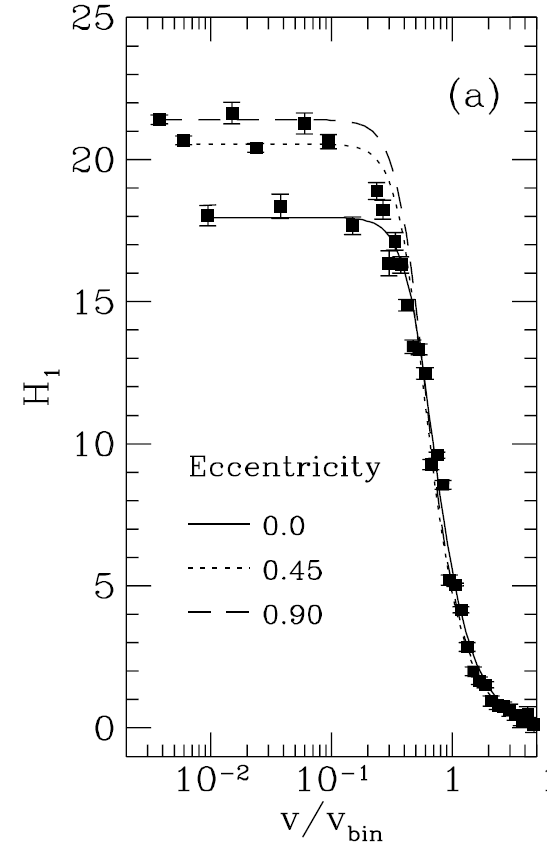
\includegraphics[width=0.5\linewidth]{H_1.png}
    \caption{This plot shows that $H_1$ is almost indipendet of the eccentricity.}
    \label{H_1 quinlann}
\end{figure}

$\mathbf{NOTE:}$ in Sesana 2010, Fig \ref{H_1 quinlann} is reported as H vs a but this agrees with the functional form of $H_1$ and $V_{bin}=\sqrt{GM_{12}/a}$.\\Therefore, the hardening rate for a circular binary have been used for all eccentricities.

\subsection{Aplication to a galaxy model}
Once stellar density $\rho$ and velocity dispersion $\sigma$ are specified, the binary BH is introduced at center of the system with a given initial eccentricity $e_0$ and separation $a_0$ such that $V_{bin}=\sigma/5$.\\The last  corresponds to a condition about $a_0$ which is model indipendent and for the binary to be soft at beginning of the integration; a BH binary is indeed called hard 
if it hardens at a constant rate, that is if $\sigma\ll \omega$ or equivalently
if $V_{bin}/\sigma \gg (1+m_1/m_2)^{1/2}$.\\Peters (1964) equation for gravitational wave emission
\begin{equation}
    \frac{da}{dt} = -\frac{64}{5} \frac{G^3 \mu m^2}{c^5 a^3} \frac{1}{(1 - e^2)^{7/2}} \left( 1 + \frac{73}{24}e^2 + \frac{37}{96}e^4 \right)
\end{equation}

\begin{equation}
    \frac{de}{dt} = -\frac{304}{15} \frac{G^3 \mu m^2}{c^5 a^4}  \frac{e}{(1 - e^2)^{5/2}} \left( 1 + \frac{121}{304}e^2 \right)
\end{equation}
are considered as well in order to compute $da/dt$ and $de/dt$.\\Despite $dM_{ej}/dt$ is computed, a and e evolution can be assumed to occur in a fixed background whenever this is negligible; the ejected mass hardly exceeds a few times $M_{12}$.\\Neverthless, the stellar mass ejection makes the binary hardening less and less efficient; once nearby stars are expelled, the hardening rate depends on the diffusion of stars back into the "Loss cone" due to two-body relaxation.\\If stars removal is efficient, correction to the density profile must be applied assuming a given rate for the process above.\\Fig.\ref{a and e quinlan} shows that the binary evolves mainly through three phases separated by two trashold destances:\begin{enumerate}
    \item $a_h=\frac{Gm_2}{4\sigma^2}$
    \item $a_{gw}$
\end{enumerate}
Quasi-circular binaries ($e_0<0.3$) remain circular with little e-growth before entering the GWs emission domain, while eccentricity increment is more important if $e_0>0.3$.






\newpage
\begin{figure}
    \centering
    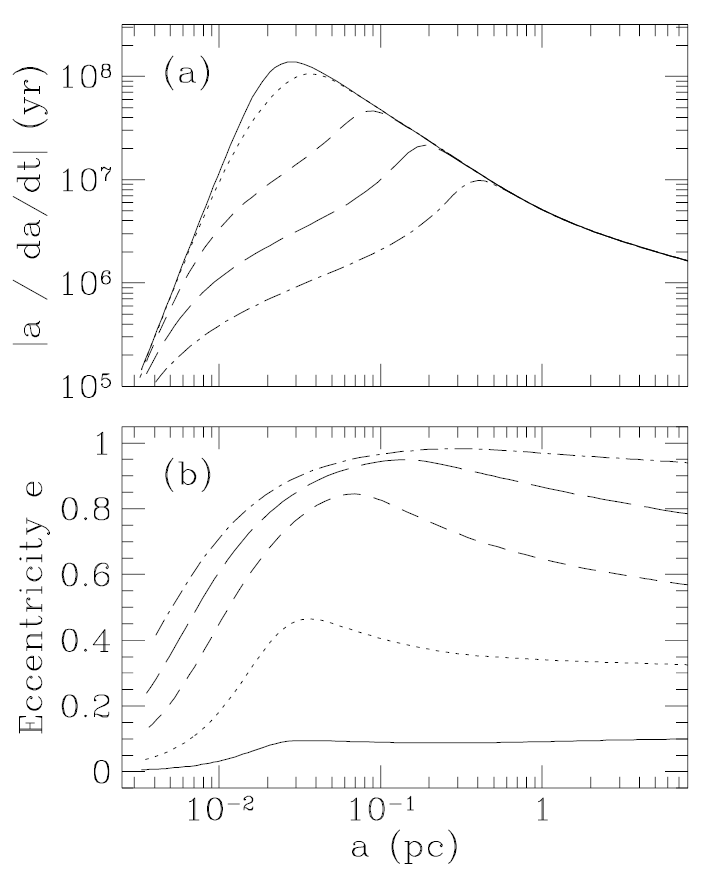
\includegraphics[width=0.5\linewidth]{a_and_e_quinlan.png}
    \caption{Eccentricity evolution. The solid line is the same as
in Fig. 7(a); the other lines assume initial eccentricities of 0.3
(dotted), 0.5, 0.7, and 0.9 (dashed-dotted).}
    \label{a and e quinlan}
\end{figure}




\section{Sesana Hybrid Model}

\subsection{Sesana Scattering Experiments}
This work \cite{Sesana_2006} is aimed at unvieling by  full three-body scattering experiments how a population of HVS form as a result of the interaction between a MBHB and ambient stars, unbound to the binary, drawn from a MB distribution . Other than the dynamical properties of these HVS, binary hardening, mass ejection rate and eccentricity growth rate $(H,J,K)$ are tracked by numerical simulations.\\Dynamical friction is efficient (especially in wet major mergers) in dragging two  massive BHs towards the innermost region of the new formed galaxy; over the time scale $t_{df}$ the binary forms and hardens  through gravitational slingshot, hence ejecting low angular momentum stars passing close to the binary. \\Following Q96 approach, the equations defining $(H,J,K)$ are (\ref{H Q96}),(\ref{J Q96}) and (\ref{K Q96}).\\At odds with Q96, where three-body scattering experiments are conducted for a fixed impact velocity, varying the binary separation and then averaging over the Maxwellian distribution, now the separation is fixed, i.e. $V_c=(GM_{12}/a)^{1/2}=const$, and the quantity $v/V_c$ is sampled over four decades, corresponding to a sampling of about four decades in binary separation.\\Each run is set by the inital configuration, corrseponding to a point in the parameter space $(q,e_0)$; the combination of binary masses ratio $q=1,1/3,1/9,1/27,1/81,1/243$ and initial eccentricity $e_0=0.01,0.3,0.6,0.9$ leads to 24 runs, involving $4\cdot10^6$ stars each.\\The (Maxwellian averaged) rates H, J,
and K derived from scattering experiments are fitted by the following functions


 \begin{equation}
     H=A(1+a/a_0)^\gamma
\end{equation}

 \begin{equation}
    J=A(a/a_0)^\alpha [(1+(a/a_0)^\beta]^\gamma
\end{equation}

\begin{equation}
    K=A(1+a/a_0)^\gamma+B.
\end{equation}

\begin{figure}
    \centering
    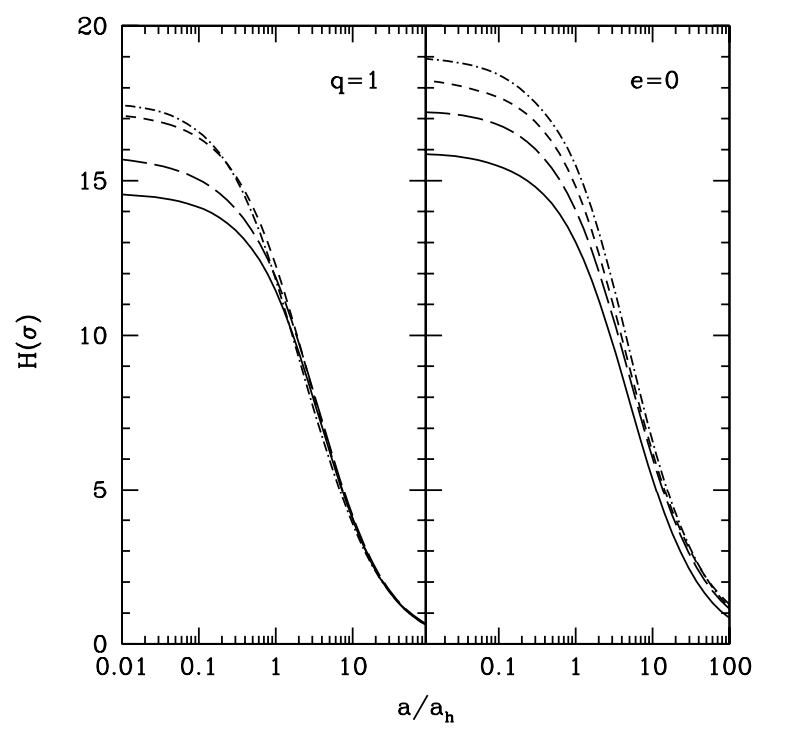
\includegraphics[width=0.5\linewidth]{H_Sesana2006.png}
    \caption{Binary hardening rate H (averaged over a Maxwellian velocity
distribution) vs. $a/a_h$. Left: $e= 0, 0.3, 0.6, 0.9$ for $q=1$. Right: q ¼ 1/3, 1/9,
1/27, and 1/81 for e ¼ 0. Line style as in Fig. 1}
    \label{H Sesana 2006}
\end{figure}


\begin{figure}
    \centering
    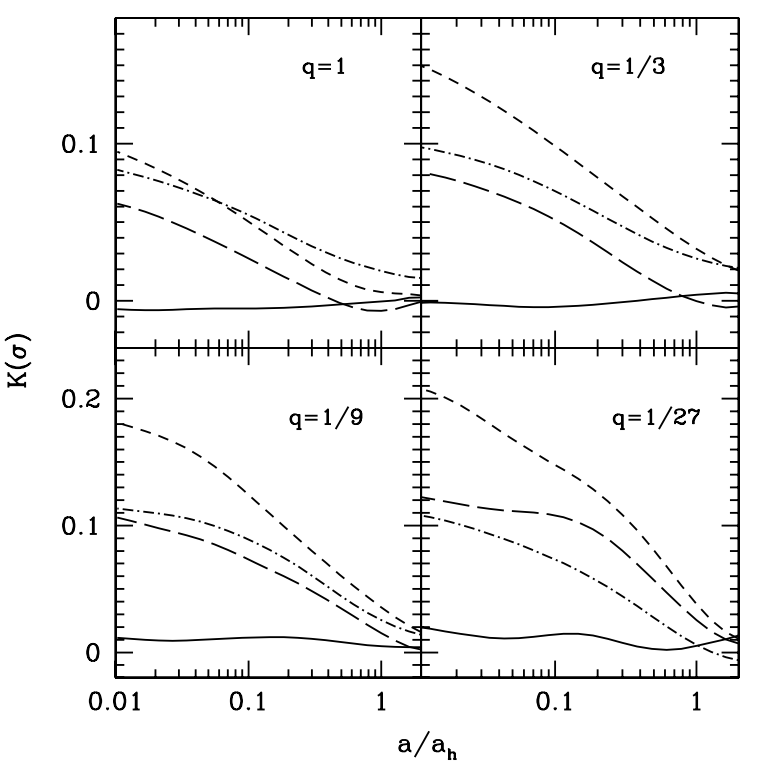
\includegraphics[width=0.5\linewidth]{K_Sesana2006.png}
    \caption{Eccentricity evolution. The solid line is the same as
in Fig. 7(a); the other lines assume initial eccentricities of 0.3
(dotted), 0.5, 0.7, and 0.9 (dashed-dotted).}
    \label{K Sesana 2006}
\end{figure}
Figure \ref{H Sesana 2006} shows that the hardening rate is nearly constant when $a<a_h$, in perfect agreement with Q96 results. Therefore hard binary can be characterised by a costant hardening rate. Additionally, $H$ decreases with $q$ (asymmetric binaries harden faster) and increases with eccentricity (circular binaries harden more slowly).\\As reported in Figure \ref{K Sesana 2006}, $K$ is close to zero at any binary separation for circular binary; if the binary is eccentric at $a_h$ already, then K (and $e$) increases monotonically with binary shrinking.\\$\mathbf{NOTE}$: in this paper the binary shrinking is studied taking into account gravitational slingshot on UNBOUND stars passing close to binary and ejected at higher velocity. In particular:
\begin{enumerate}
    \item the ejection criterion relies on the stellar background model (here SIS stellar Bulge is considered)
    \item The stellar background is assumed to be fixed; this approximation holds if the ejected mass does not exceed a trashold
    \item Binary shrinking requires low angular momentum stars as they havo to pass closer and closer to the binary BHs for slingshot to be effective; however from $a<a_h$ the fraction of stars with these properties, populating the so called "Loss cone", is very small. Being depletd by three-body encounters, binary hardening when binary is hard depends on the efficiency of loss cone refilling.
\end{enumerate}
 
Bound stars \cite{Sesana_2008}     ,\cite{Sesana_2010}
\newpage
\subsection{Sesana 2010 Results and  Comparison}
As confirmed by observations of galaxies hosting a dynamically evolved BH binary, stellar scouring by binary hardening seems to imprint an inner cusp to the original stellar background. Motivated by this emerging picture, Sesana \cite{Sesana_2010} adopted a stellar density profile matching a SIS outside the binary influence radius $r_{inf}$ and a power low distribution inside; in formulae:
\begin{flushleft}\label{Sesana_2010 stellar cusp profile}
  $
  \left\{
  \begin{aligned}
  \rho(r)=\rho_{inf}\left(\frac{r}{r_{inf}}\right)^{-\gamma} \qquad if \quad r<r_{inf}\\
  \\ \rho(r)=\frac{\sigma^2}{2\pi G r^2} \qquad if \quad r>r_{inf}
  \end{aligned}
  \right.
  $
  \end{flushleft}
Here $\sigma$ indicates the radius-indipendent velocity dispersion of SIS model and it assumed to be a function of binary mass $M=M_1+M_2$, such that $q=M_2/M_1<1$, through \cite{Tremaine_2002}
\begin{equation}\label{Tremaine_2002 M_bh}
    M_6=0.84\sigma_{70}^4.
\end{equation}
Dynamical friction is efficient in dragging two BHs down to the separation $a_0$ at which the enclosed stellar mass
in the binary is twice the mass of the secondary BH, i.e.  
\begin{equation}\label{Sesana_2010 a_0}
    a_0=(3-\gamma)\frac{GM}{\sigma^2}\left(\frac{q}{1+q}\right)^{1/(3-\gamma)}=r_{inf}\left(\frac{q}{1+q}\right)^{1/(3-\gamma)},
\end{equation}
and is adopted as starting point of the numerical integration.\\Hereafter, three competing mechanisms are involved:
\begin{enumerate}
    \item Bound cusp erosion:
    \begin{equation}\label{Sesana_2010 da/dt BOUND}
    \left.\frac{da}{dt}\right|_{b} = -\frac{2a^2}{G M_1 M_2} \int_0^\infty \Delta \mathcal{E}\frac{d^2 N_{\mathrm{ej}}}{da_\star dt} da_\star
\end{equation}

\begin{equation}\label{Sesana_2010 de/dt BOUND}
    \left.\frac{de}{dt}\right|_{b}= \int_0^\infty \Delta e \frac{d^2 N_{\mathrm{ej}}}{da_\star dt} da_\star
\end{equation}
    
\item   Slingshot of unbound stars:
\begin{equation}
    \left.\frac{da}{dt}\right|_{u} = -\frac{a^2 G \rho}{\sigma} H
\end{equation}

\begin{equation}
    \left.\frac{de}{dt}\right|_{u} = \frac{a G \rho}{\sigma} H K
\end{equation}

\item Gravitational waves emission \cite{Peters_1963}:
\begin{equation}
    \left.\frac{da}{dt}\right|_{\mathrm{GW}} = -\frac{64}{5} \frac{G^3}{c^5} \frac{M_1 M_2 M}{a^3 (1 - e^2)^{7/2}} \left( 1 + \frac{73}{24} e^2 + \frac{37}{96} e^4 \right)\equiv -\frac{64}{5} \frac{G^3}{c^5} \frac{M_1 M_2 M}{a^3}F(e)
\end{equation}


\begin{equation}
    \left.\frac{de}{dt}\right|_{\mathrm{GW}} = -\frac{304}{15} \frac{G^3}{c^5} \frac{M_1 M_2 M}{a^4 (1 - e^2)^{5/2}} e \left( 1 + \frac{121}{304} e^2 \right)
\end{equation}

\end{enumerate}
Being indipendet of each other, by superposition, we can put
the pieces together and the evolution of the binary obeys to


\begin{equation}\label{Sesana_2010 da/dt TOT}
    \frac{da}{dt} = \sum_i \left.\frac{da}{dt}\right|_i
\end{equation}

\begin{equation}\label{Sesana_2010 de/dt TOT}
    \frac{de}{dt} = \sum_i \left.\frac{de}{dt}\right|_i.
\end{equation}
Besides, an equal number of regimes can be introduced whereby one single mechanism is dominant over the others; lengthscale boundaries are $a_0$,
\begin{equation}\label{Sesana_2010 a_h}
    a_h\approx\frac{1}{4(3-\gamma)}\left(\frac{q}{1+q}\right)^{(2-\gamma)(3-\gamma)}
\end{equation}
and 
\begin{equation}
    a_{GW}=4\left[\frac{128\pi(3-\gamma) F(e)}{5H}\right]^{1/5}\frac{\sigma}{c}q^{-4/5}(1+q)^{3/5}a_h
\end{equation}
respectively.\\We recall that
\begin{equation}\label{Sesana_2010 rho_inf}
    \rho_{inf}=\frac{\sigma^2}{2\pi G r_{inf}^2}
\end{equation}
and that setting $\rho=\rho_{inf}$ inside Equation (\ref{da/dt UNBOUND}) is equivalent to impose a full loss-cone outside the binary sphere of influence during the unbound phase; the effects due to different normalizations could be explored.\\Sesana \cite{Sesana_2010} explored a relatively wide region of the phase space related to the initial configuration of the binary; here, we report the comparison between Sesana and our evolutionary track for $(q,\gamma,e_0,M)=(1,1.5,0.1,10^5 M_\odot)$.\\This kind of configuration, among the analyzed ones, is quite relevant to our studies on IMBH binaries at high z as they are expected to be more symmetric then their local universe cousins. As pointed out at the end of Section \ref{sec:Loss Cone}, $a_h$ and $r_{inf}$ are of the order of $\sim GM/\sigma^2$ and the bound cusp erosion process can be suppressed at first istance.\\The estimate of the hardening radius, below which $a_h$ is nearly costant, and the best fitting parameters in Table 1 \cite{Sesana_2006} allows us to find 
 \begin{equation}\label{Sesana_2006 H fit}
     H=A(1+a/a_0)^\gamma;
\end{equation}
the function is shown in Figure \ref{Sesana comparison H plot}.
\begin{figure}[H]
    \centering
    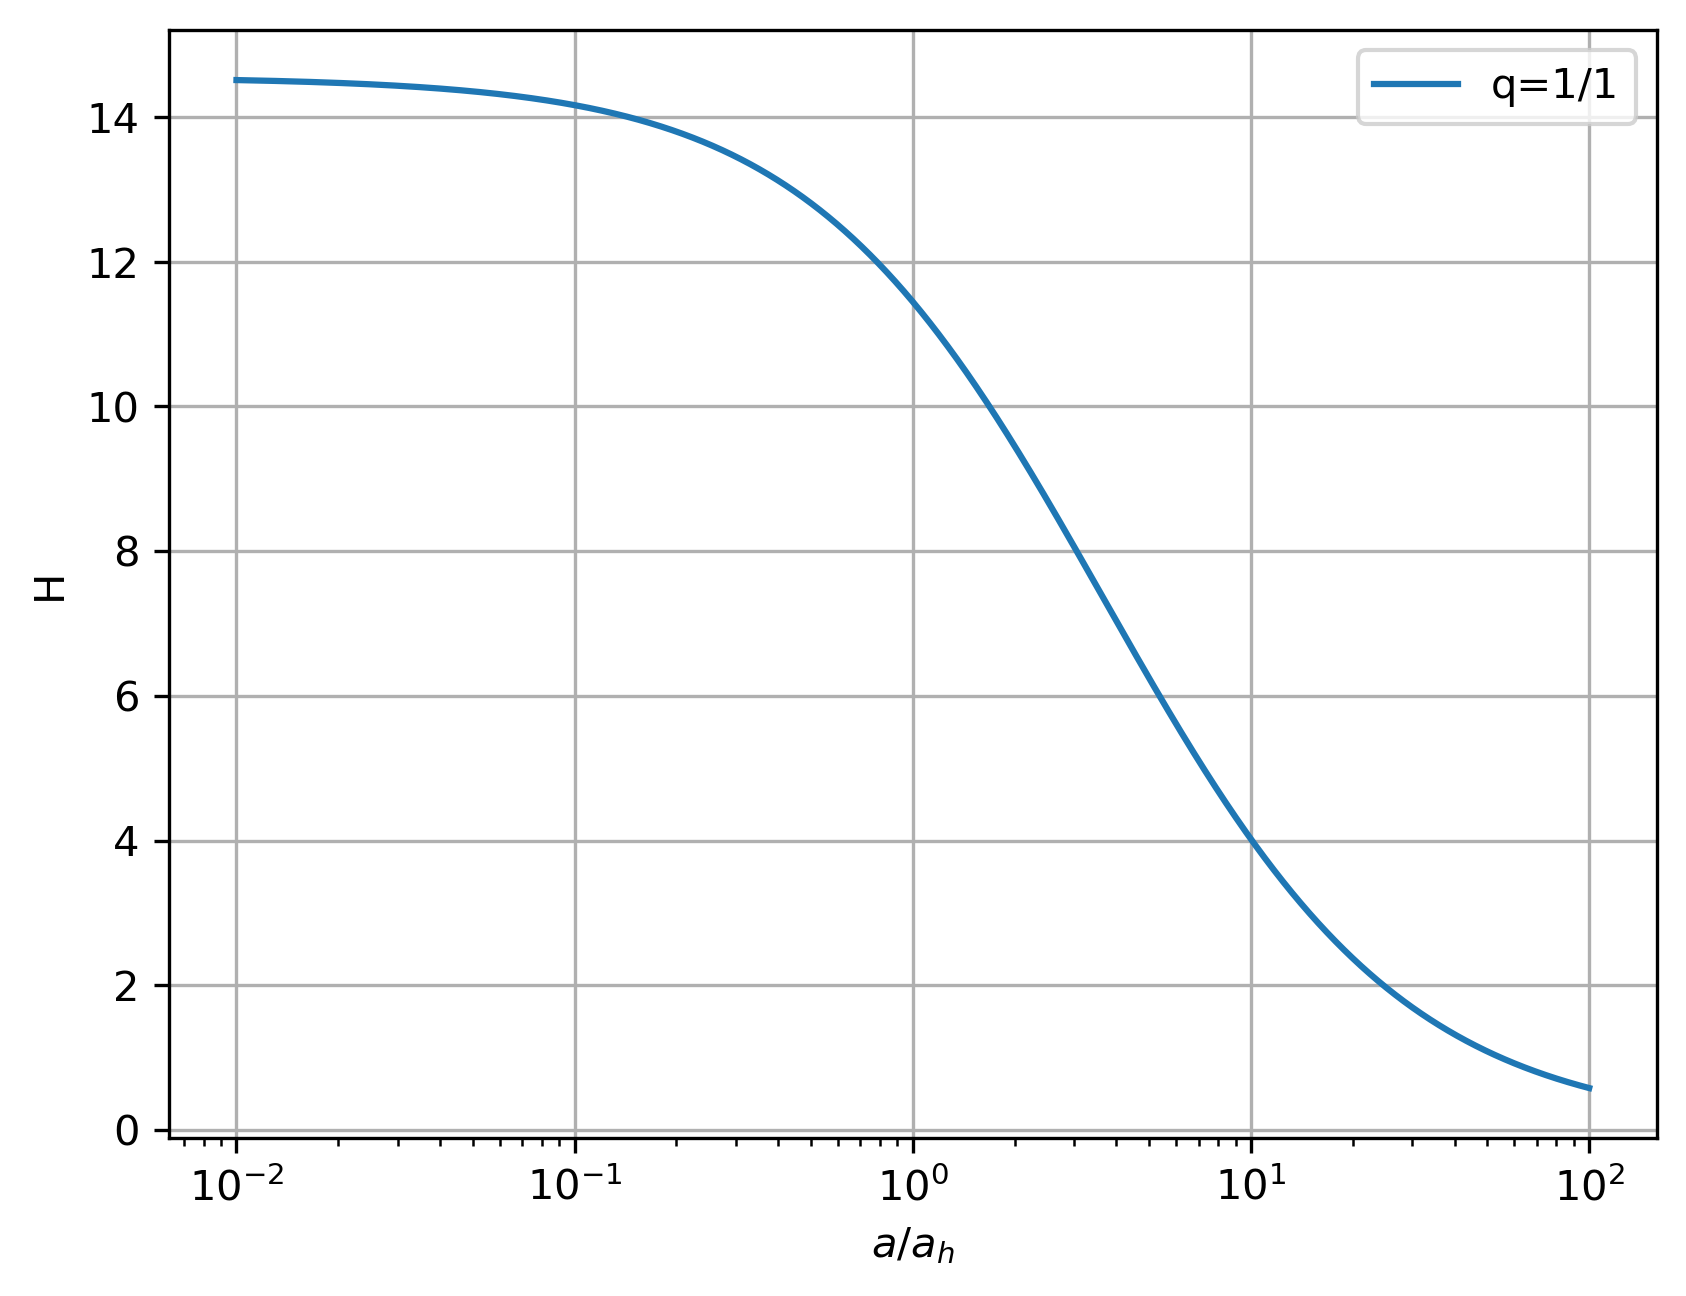
\includegraphics[width=0.5\linewidth]{H_vs_a.png}
    \caption{H as a function of $a$ expressed in $a_h$ units.}
    \label{Sesana comparison H plot}
\end{figure}






\begin{figure}[H]
    \centering
    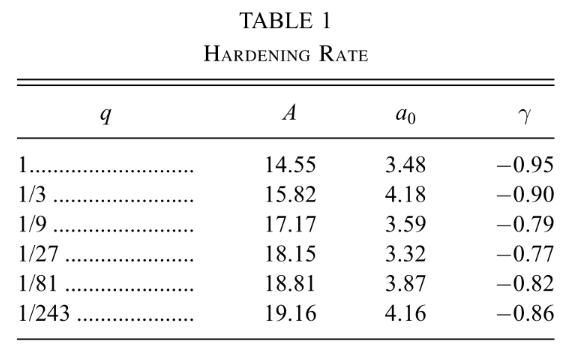
\includegraphics[width=0.5\linewidth]{Sesana_2006_Table_1.png}
    \caption{Note: $a_0$ is given in $a_h$ units.}
    \label{Sesana_2006_Table_1}
\end{figure}
Similarly, by interpolation over the eccentricty grid of Table 3 \cite{Sesana_2006} parameters, it is obtained
 \begin{equation}\label{Sesana_2006 K fit}
    K=A(1+a/a_0)^\gamma+B.
\end{equation}

\begin{figure}[H]
    \centering
    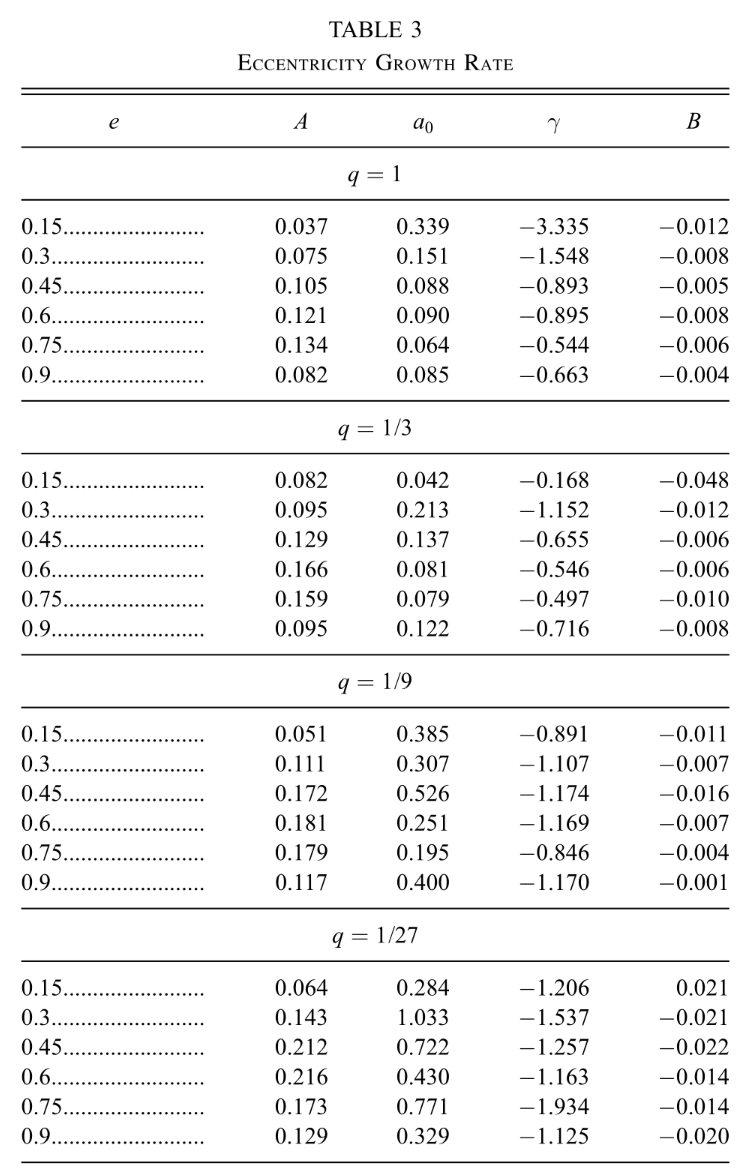
\includegraphics[width=0.5\linewidth]{Sesana_2006_Table_3.png}
    \caption{Note: $a_0$ is given in $a_h$ units.}
    \label{Sesana_2006_Table_3}
\end{figure}

Figure \ref{A of K fit Sesana comparison},\ref{a_0 of K fit Sesana comparison}, \ref{gamma of K fit Sesana comparison} and \ref{B of K fit Sesana comparison} report the results of this mathematical operation.


\begin{figure}[H]
    \centering
    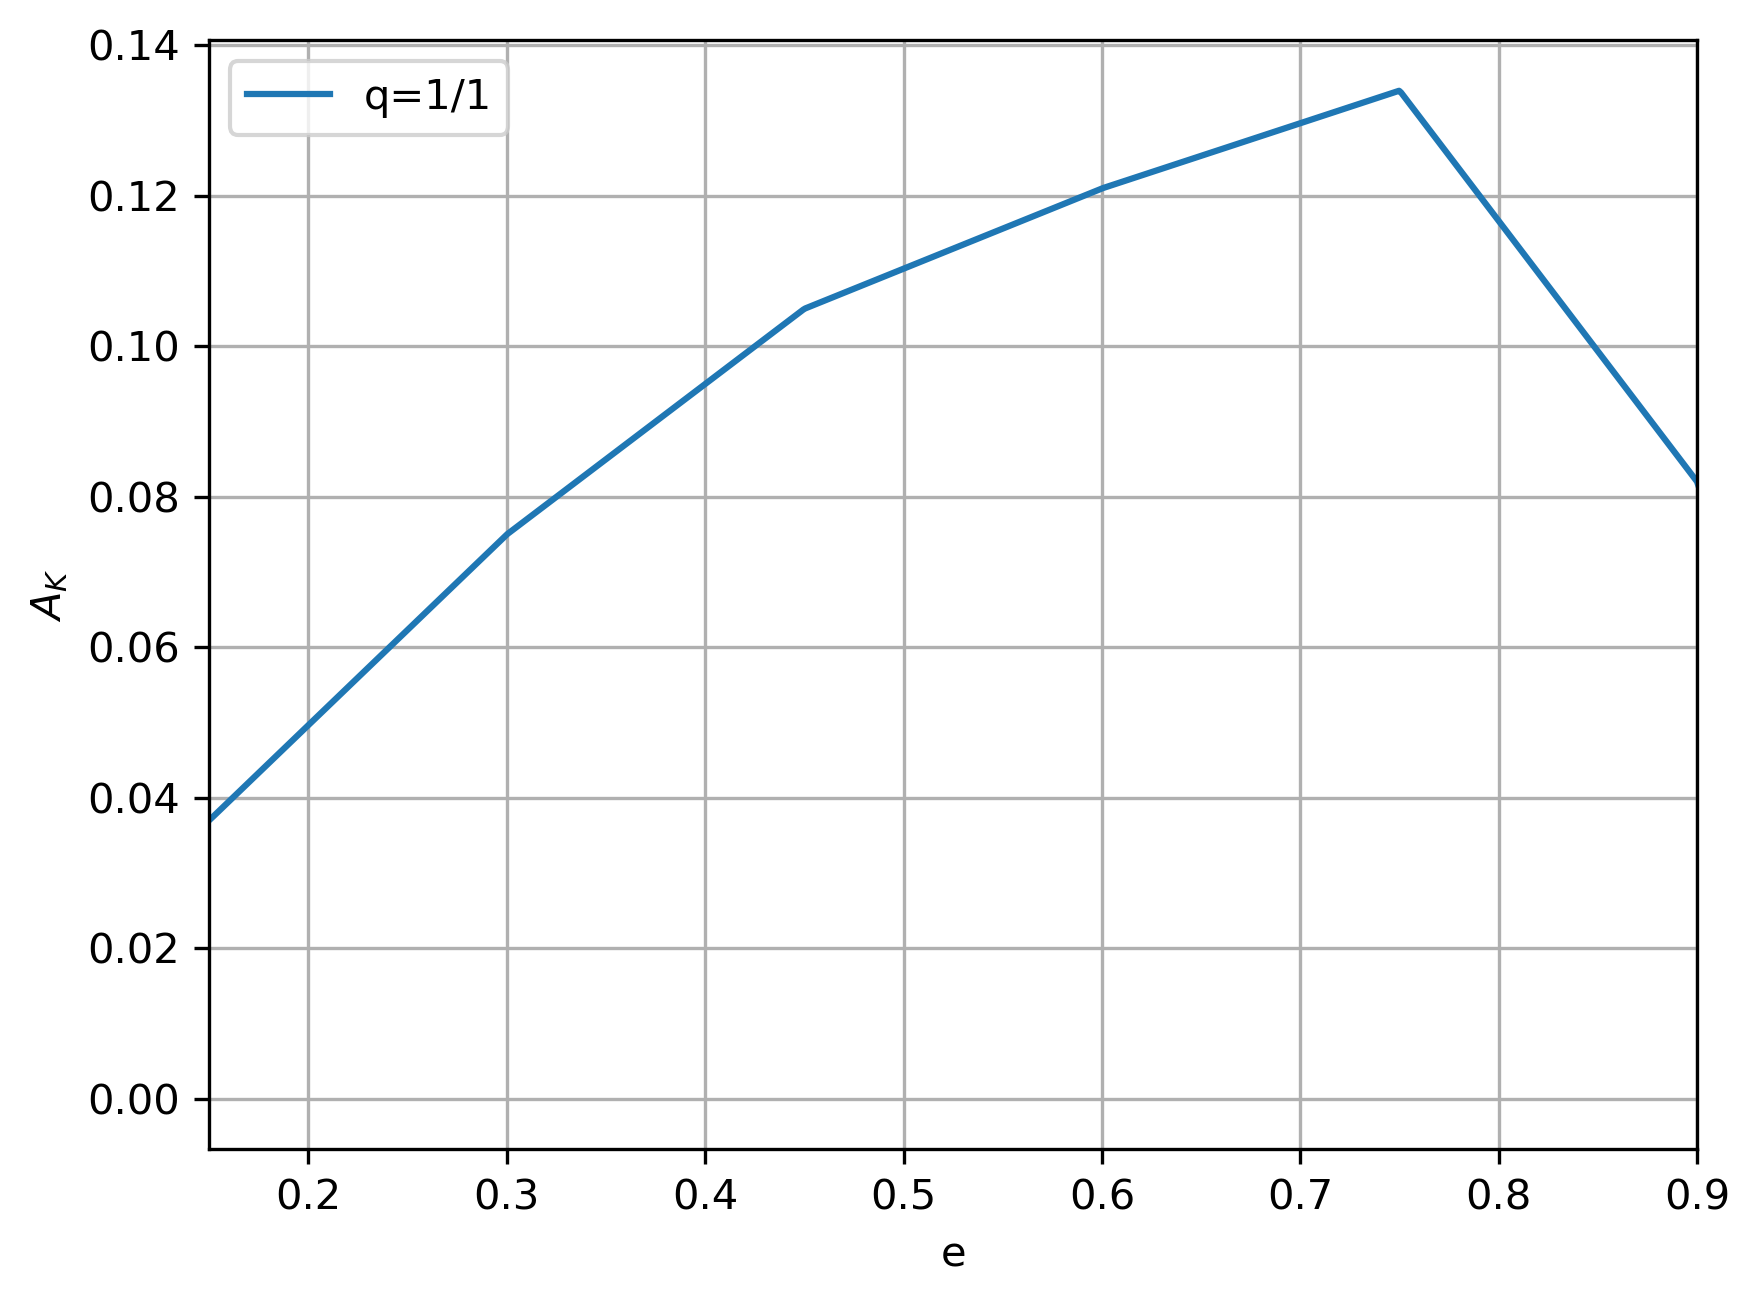
\includegraphics[width=0.5\linewidth]{A_K_vs_e.png}
    \caption{$A$ as a function of $e$ derived by interpolation of grid points.}
    \label{A of K fit Sesana comparison}
\end{figure}


\begin{figure}[H]
    \centering
    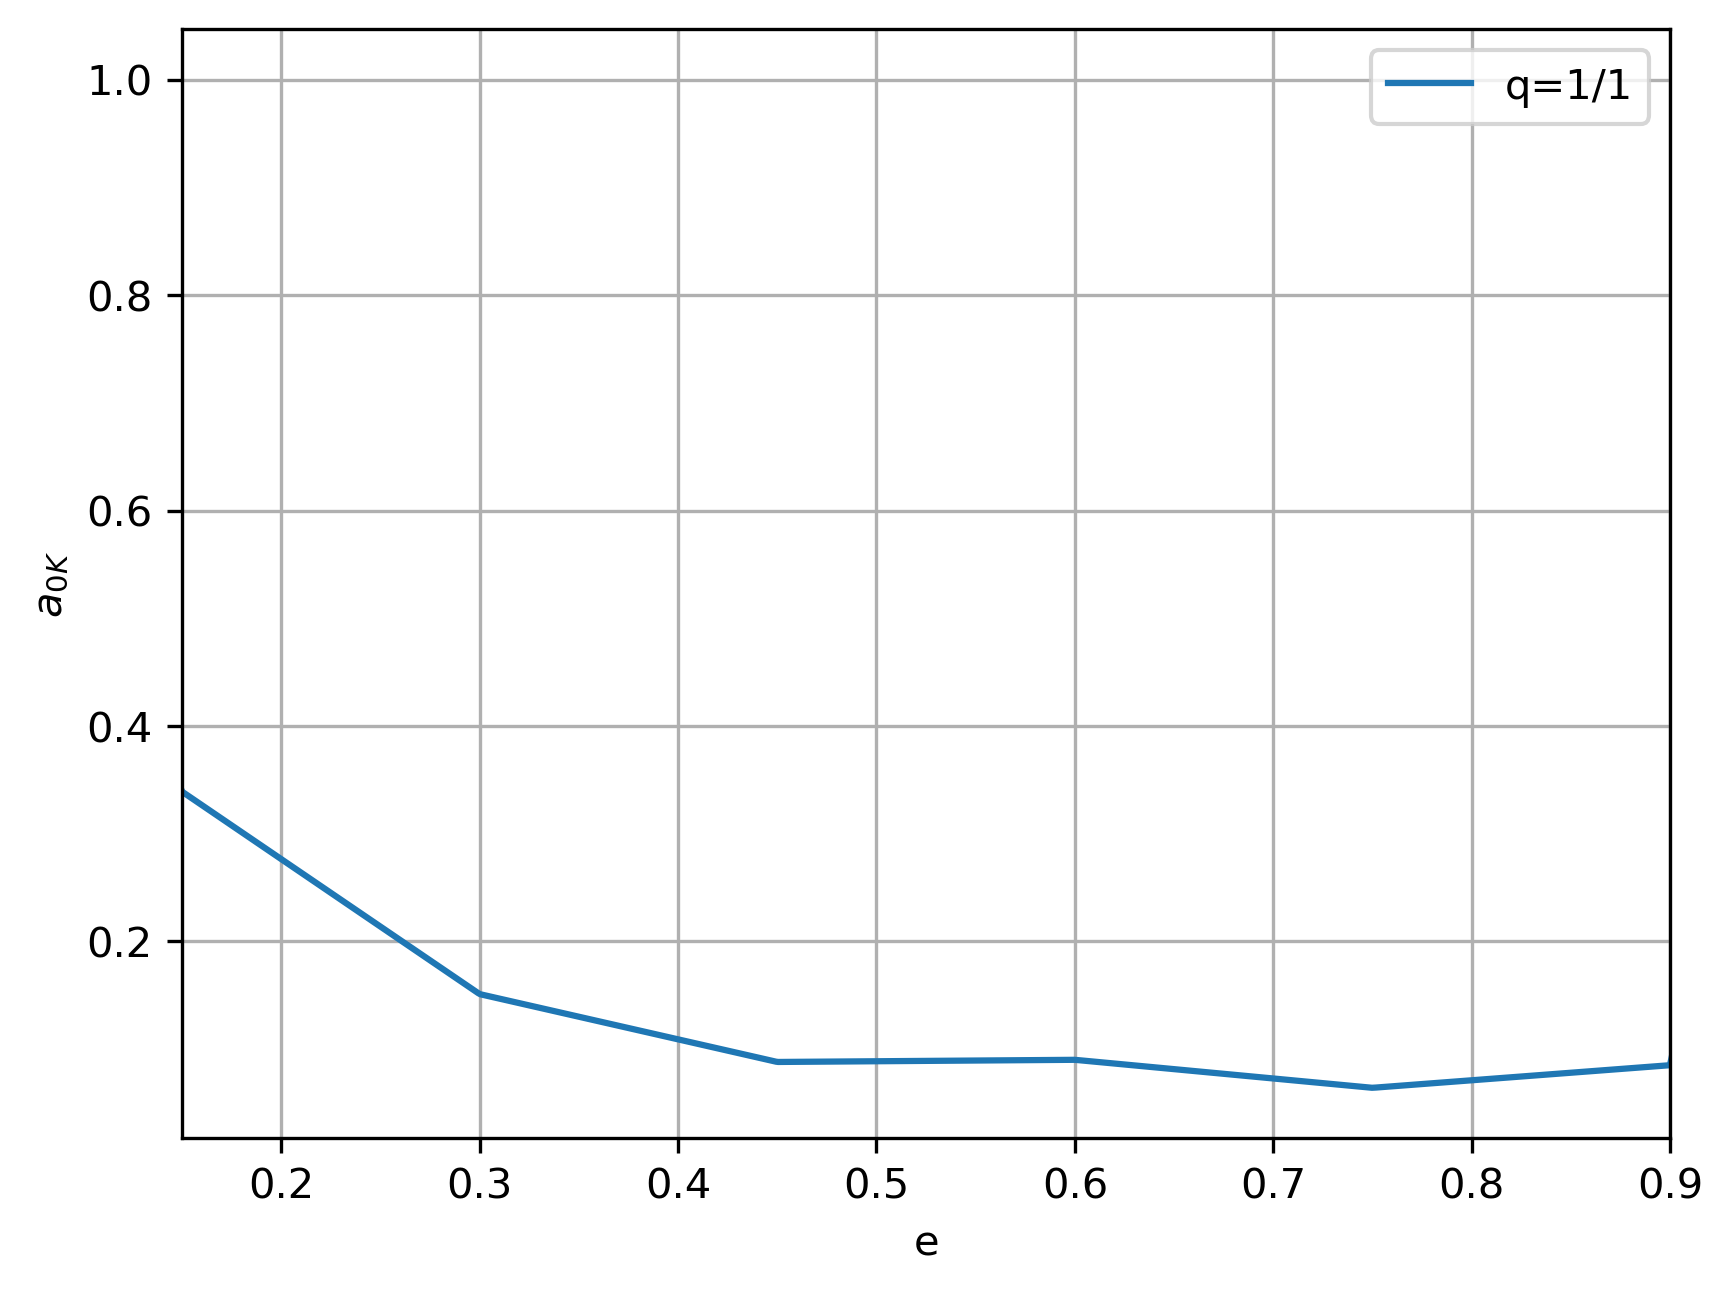
\includegraphics[width=0.5\linewidth]{a0_K_vs_e.png}
    \caption{$A$ as a function of $e$ derived by interpolation of grid points.}
    \label{a_0 of K fit Sesana comparison}
\end{figure}


\begin{figure}[H]
    \centering
    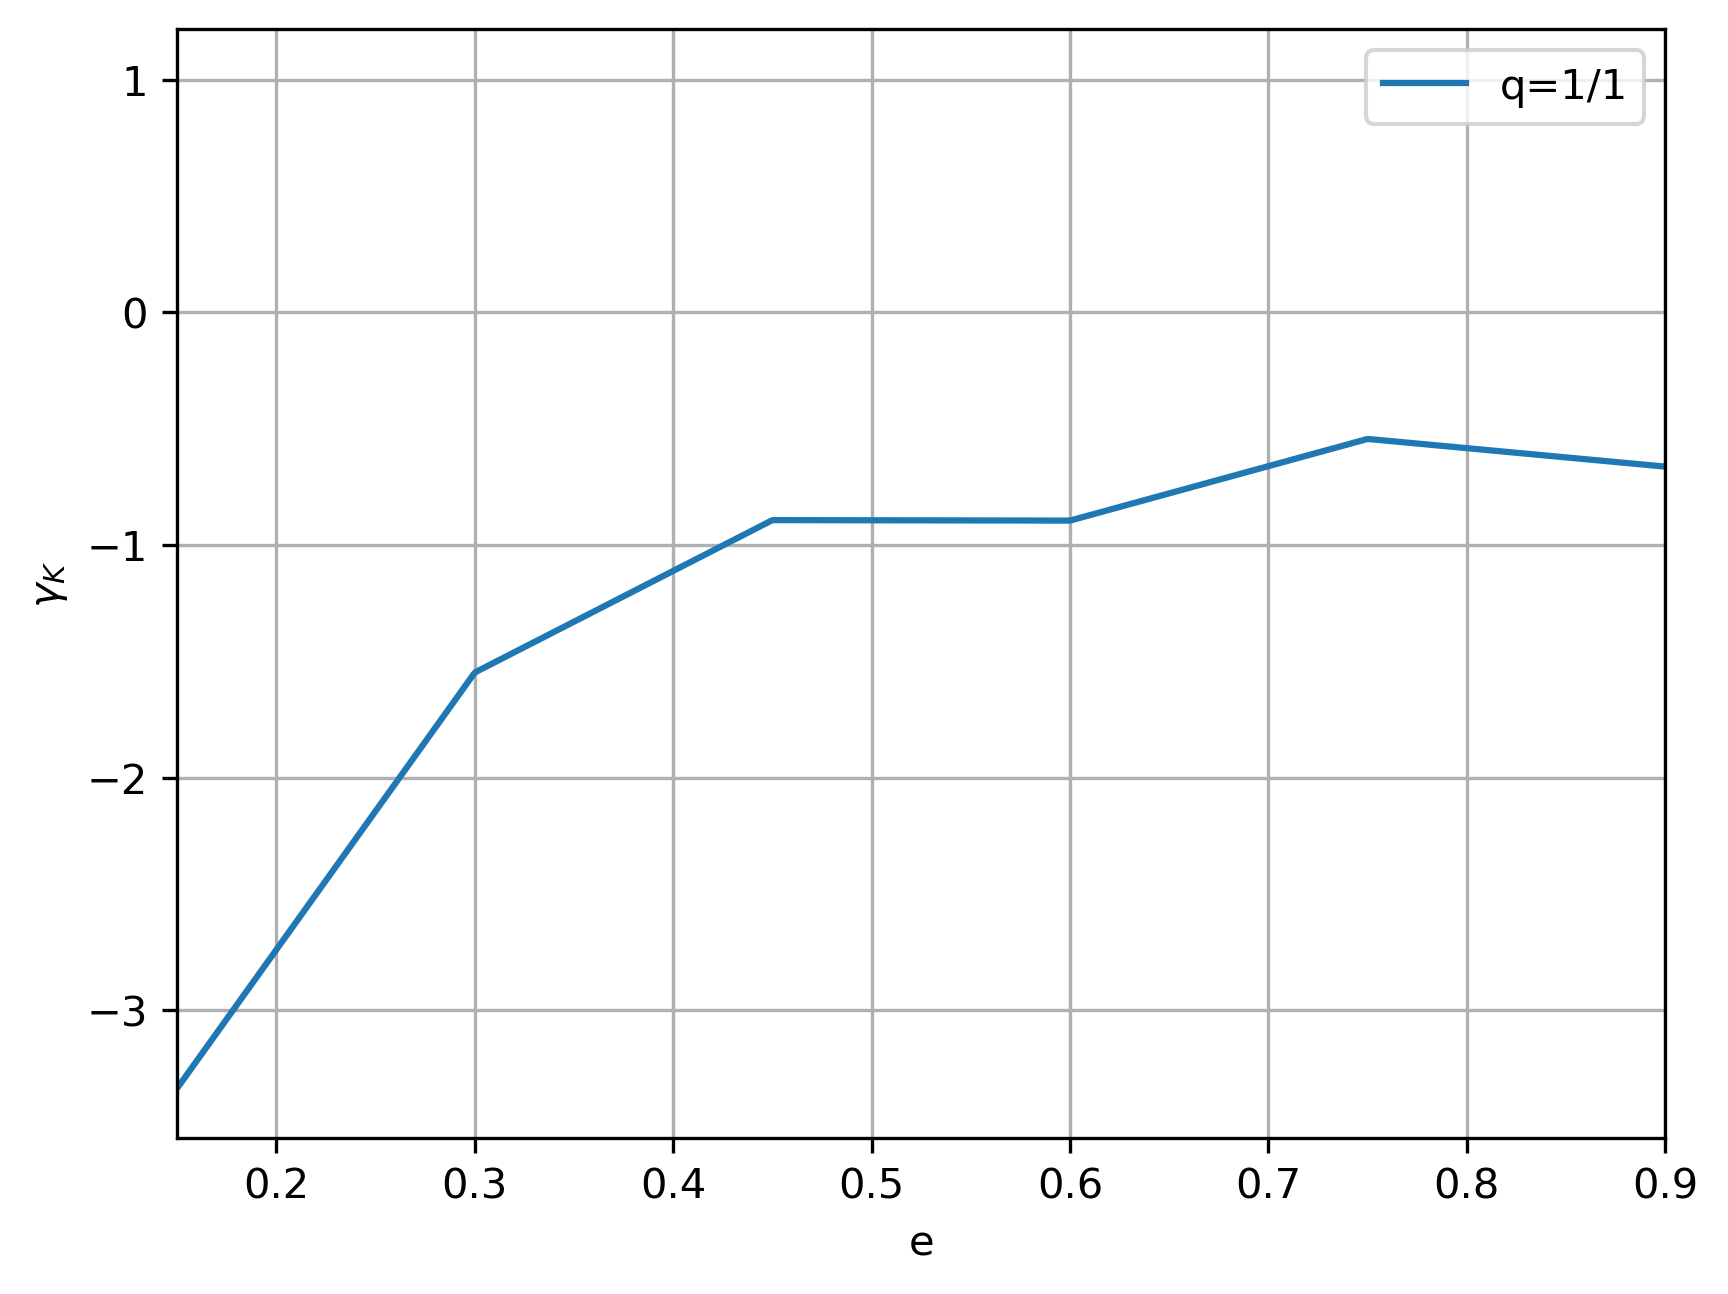
\includegraphics[width=0.5\linewidth]{gamma_K_vs_e.png}
    \caption{$\gamma$ as a function of $e$ derived by interpolation of grid points.}
    \label{gamma of K fit Sesana comparison}
\end{figure}






\begin{figure}[H]
    \centering
    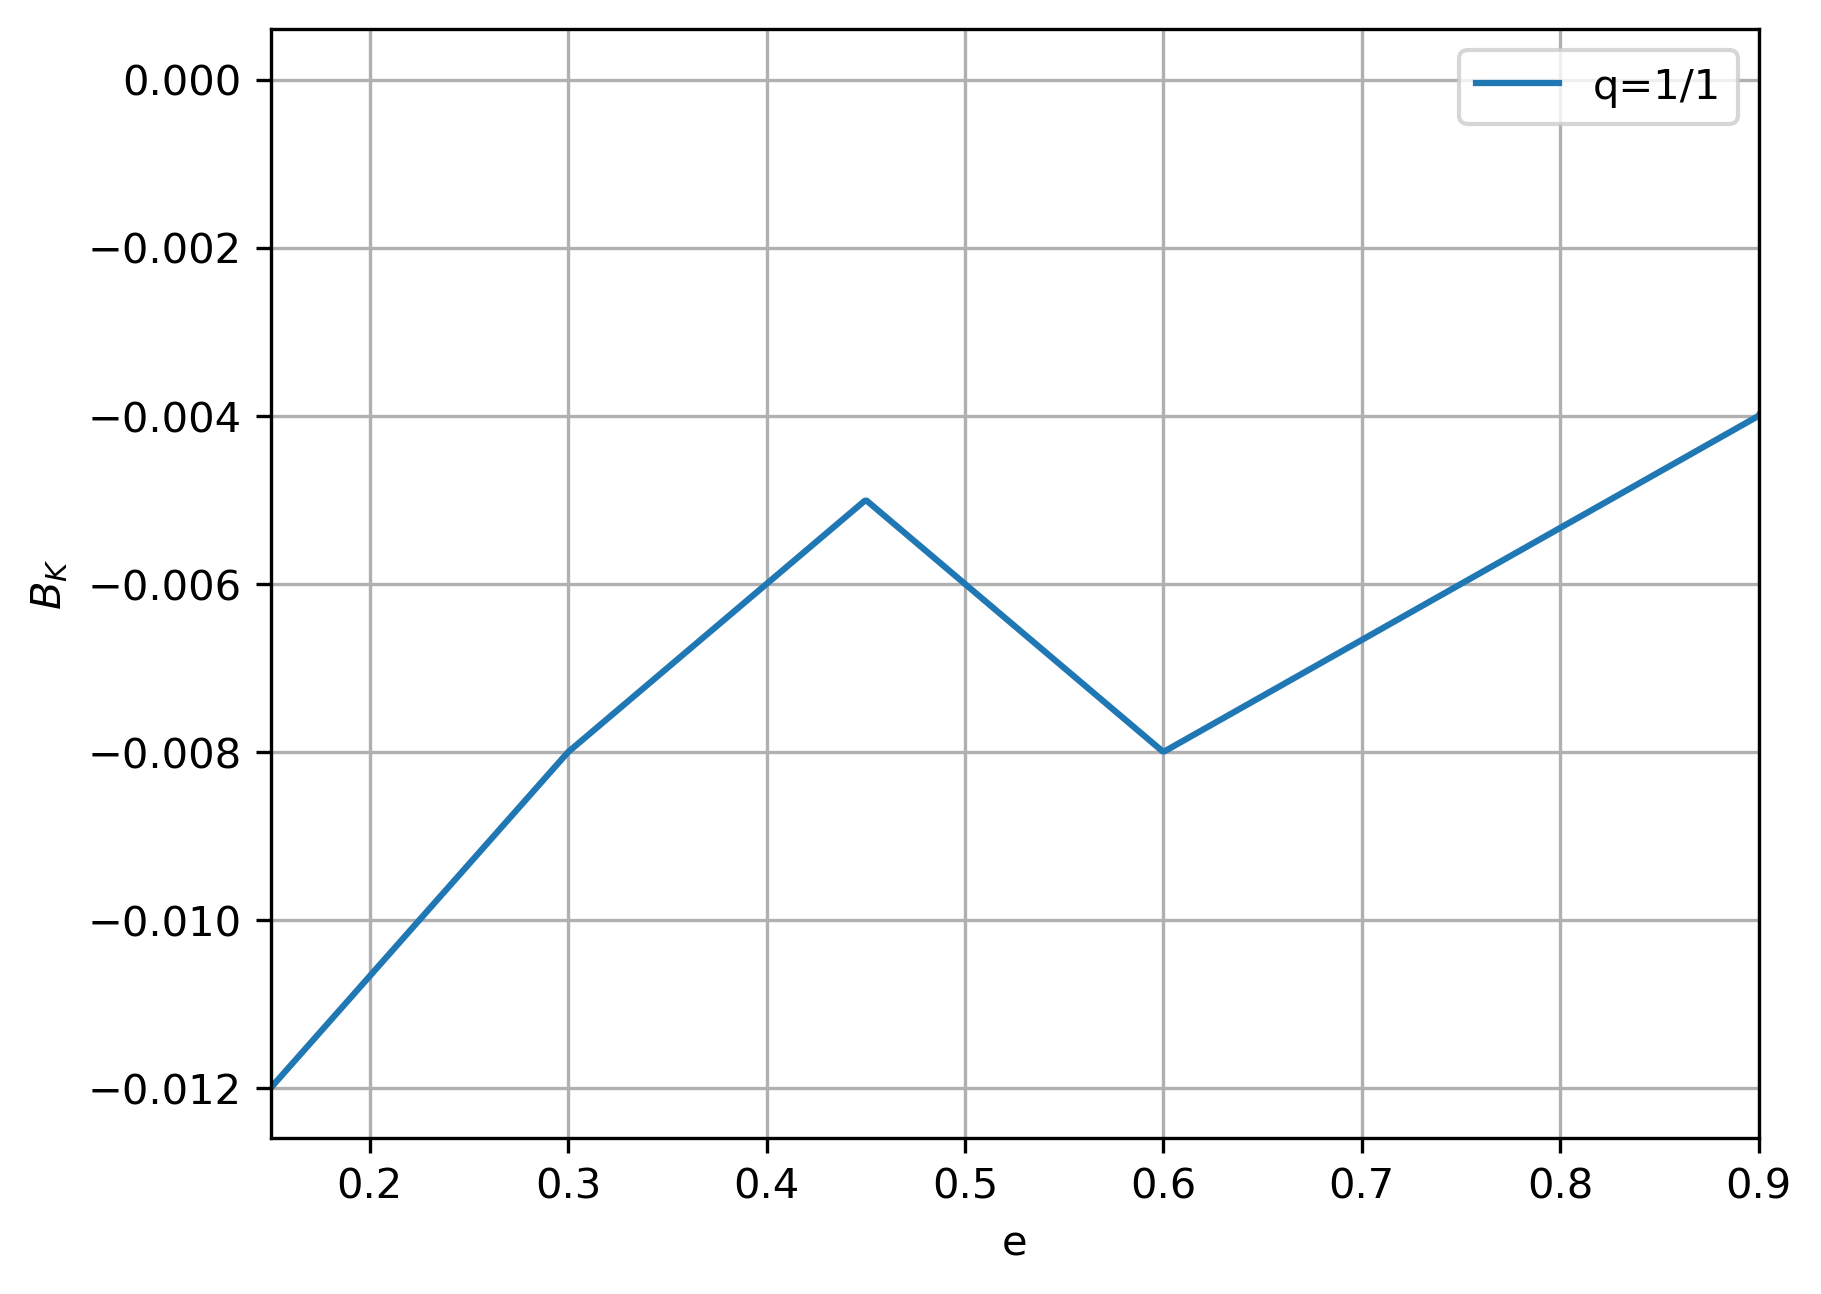
\includegraphics[width=0.5\linewidth]{B_K_vs_e.png}
    \caption{$B$ as a function of $e$ derived by interpolation of grid points.}
    \label{B of K fit Sesana comparison}
\end{figure}

Therefore, at odds with $H$, $K$ is a function of $(a,e)$; we list below the plots of the 1-D functions $K(a)=K(a,e_0)$ and $K(e)=K(a_h,e)$.


\begin{figure}[H]
    \centering
    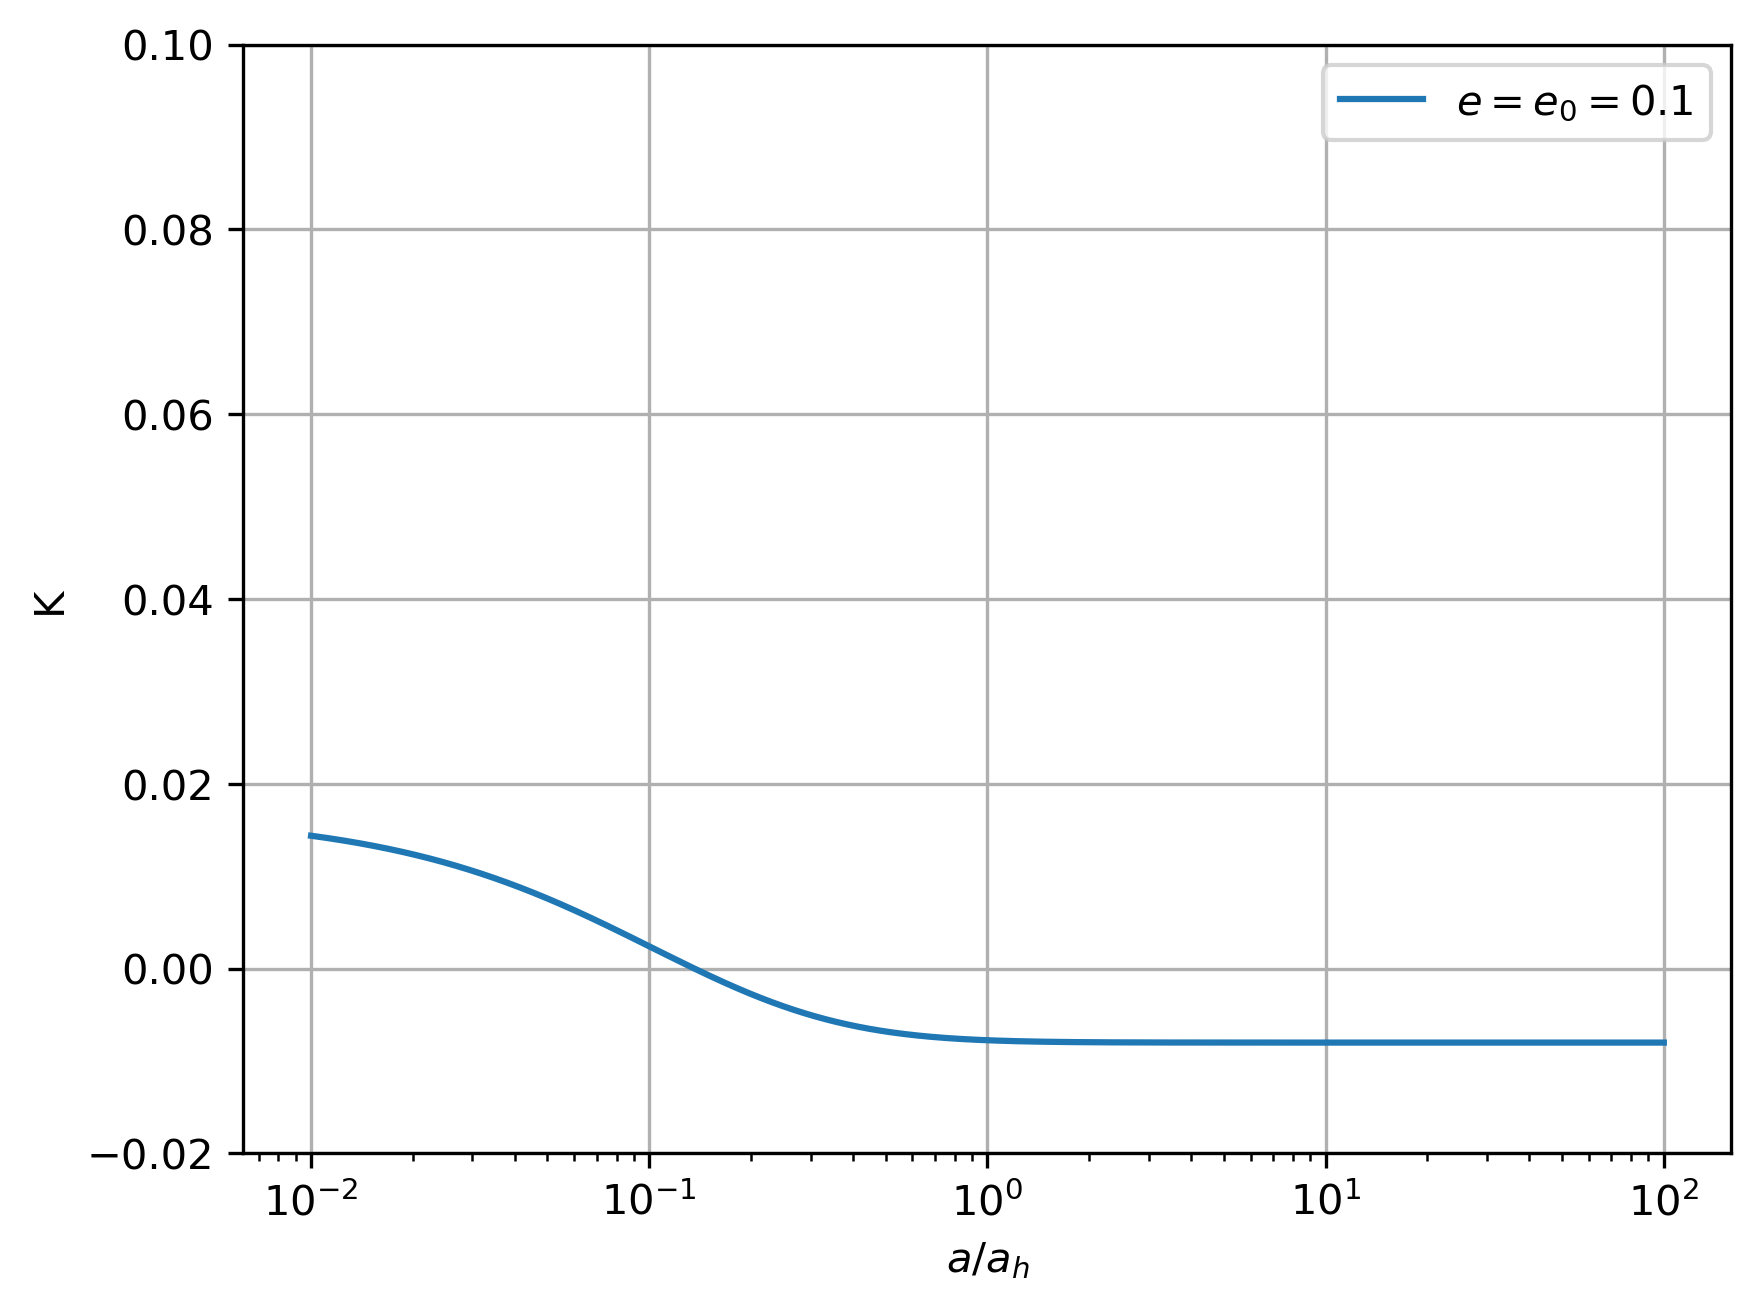
\includegraphics[width=0.5\linewidth]{K_vs_a.png}
    \caption{}
    \label{K vs a Sesana comparison}
\end{figure}


\begin{figure}[H]
    \centering
    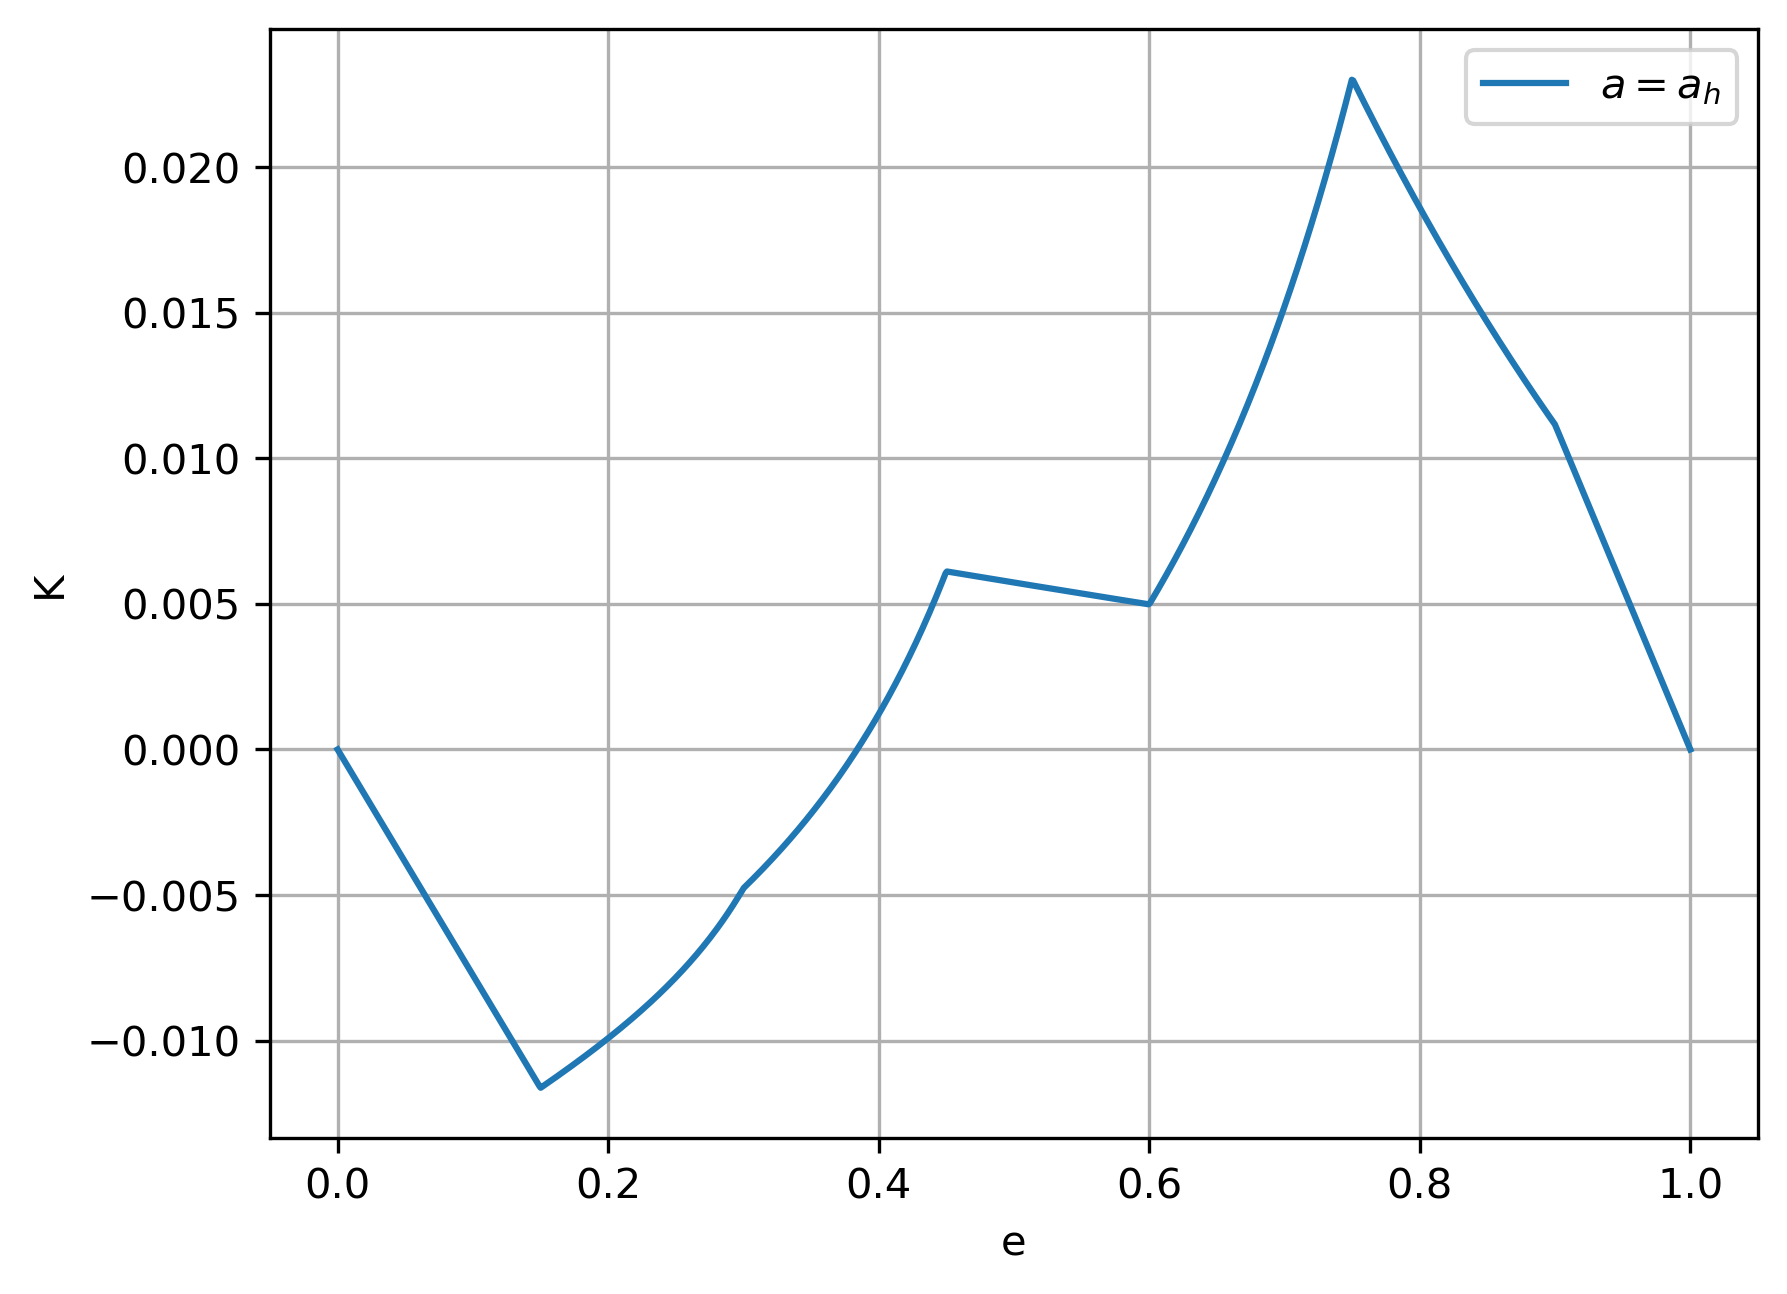
\includegraphics[width=0.5\linewidth]{K_vs_e.png}
    \caption{}
    \label{K vs e Sesana comparison}
\end{figure}
We anticipate that Equations (\ref{Sesana_2010 da/dt TOT}) and (\ref{Sesana_2010 de/dt TOT}) will be integrated with the help of RK(4) and $dK/de$ is needed as well; Figure \ref{dK/de vs e Sesana comparison} depicts the step-like function.

\begin{figure}[H]
    \centering
    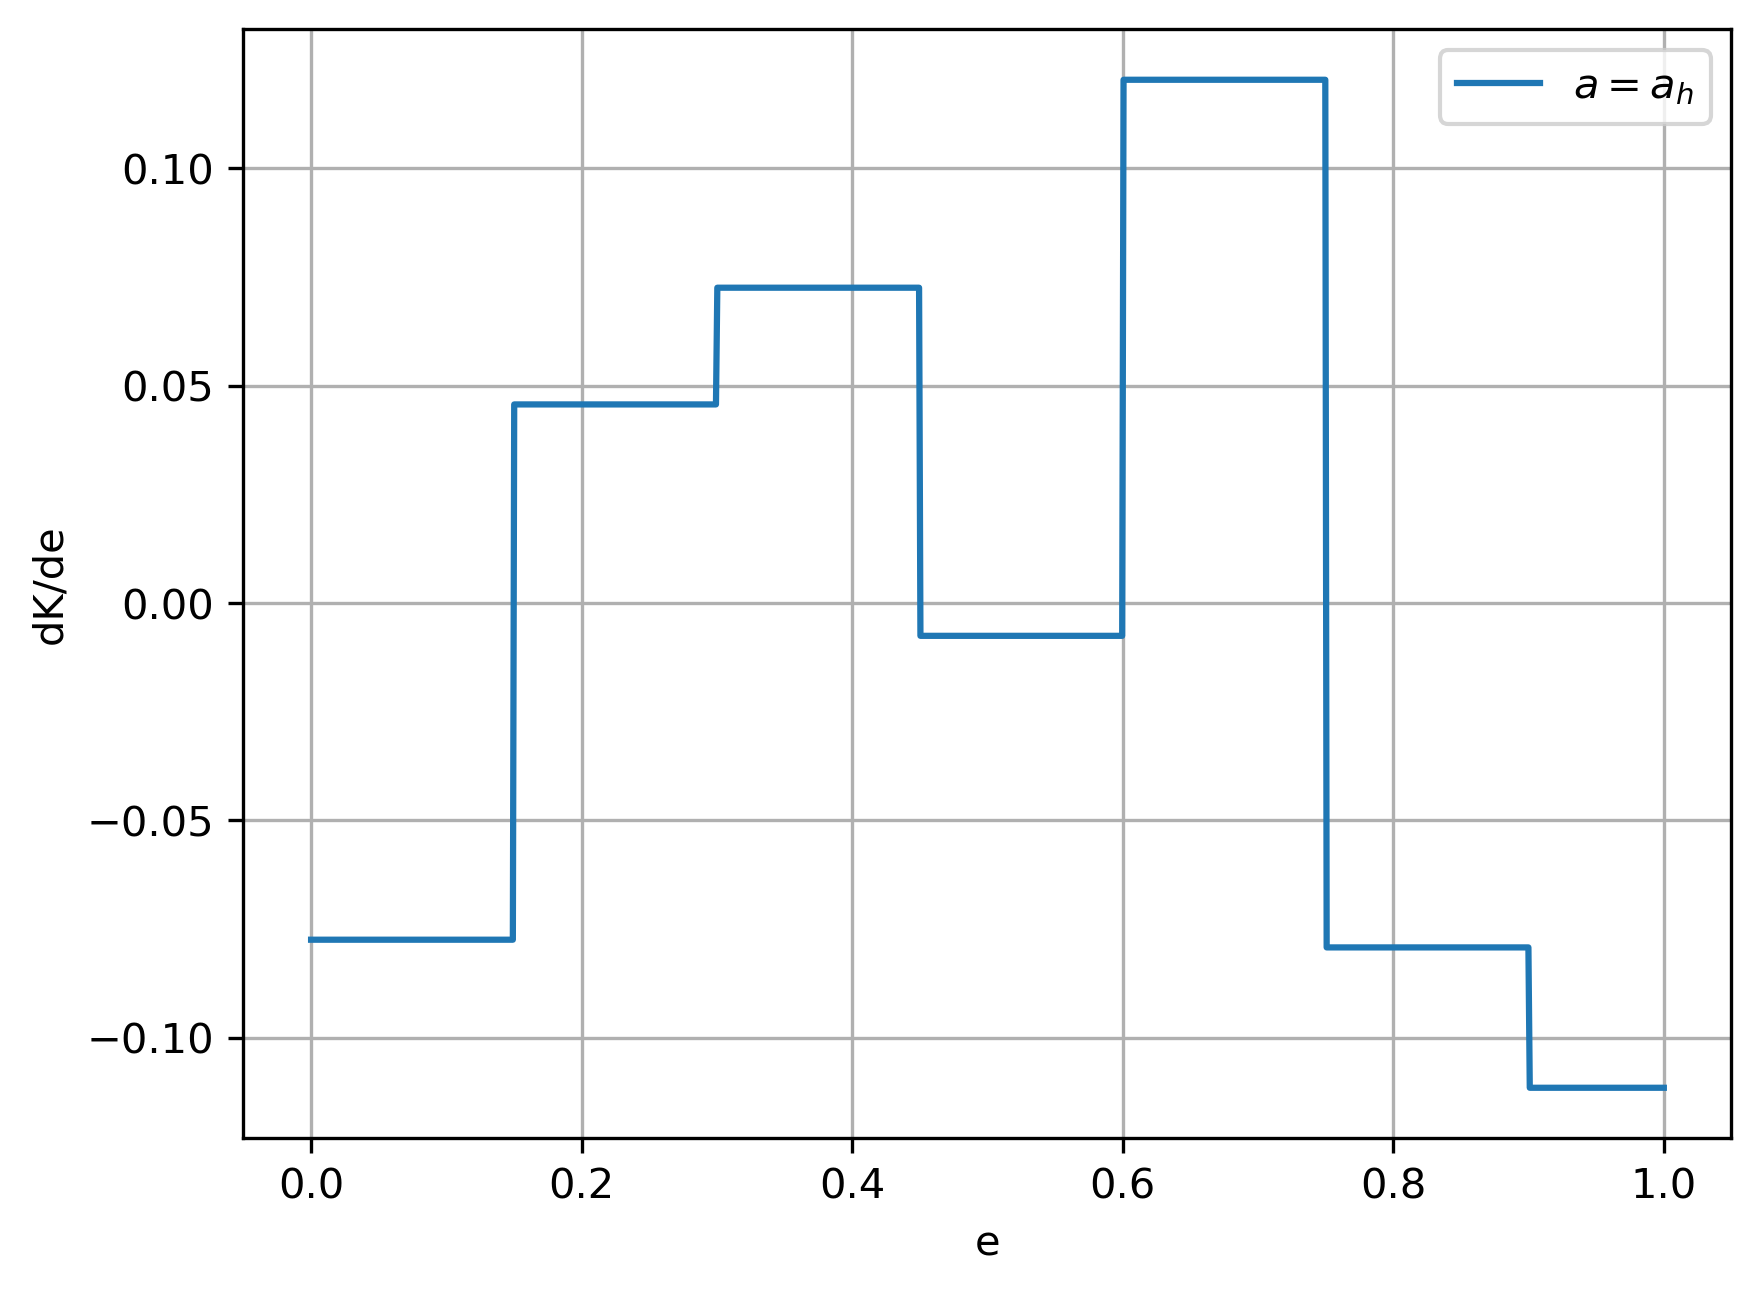
\includegraphics[width=0.5\linewidth]{dK_de_vs_e.png}
    \caption{}
    \label{dK/de vs e Sesana comparison}
\end{figure}
The time step is adjusted at each iteration according to the prescription
\begin{equation}
    \Delta t \le  min\left \{\frac{2.79}{|\lambda_i|}\right\} \qquad \forall i=1,N
\end{equation}
where $\lambda_i$ are the Jacobian $\mathbf{J}$ eigenvalues. The elements of this matrix are:
\begin{equation}\label{J_11 of Sesana comparison}
    J_{11}=\left. \frac{da}{dt}\right|_u\left(\frac{2}{a}+\frac{\gamma}{a+a_0a_h}\right)-\left.\frac{da}{dt}\right|_{gw}\left(\frac{3}{a}\right)
\end{equation}


\begin{equation}\label{J_12 of Sesana comparison}
    J_{12}=\left. \frac{da}{dt}\right|_{GW}\left(\frac{{7e}}{1-e^2}+\frac{73e/12+37e^3/24}{1+73e^2/24+37e^4/96}\right)
\end{equation}





\begin{equation}\label{J_21 of Sesana comparison}
    J_{21}=\left.\frac{de}{dt}\right|_u\left(\frac{1}{a}+\frac{\gamma_H}{a+a_{0,H}a_h}+\frac{\gamma_K}{a+a_{0,K}a_h}\right)-\left.\frac{de}{dt}\right|_{GW}\left(\frac{4}{a}\right)
\end{equation}


\begin{equation}\label{J_22 of Sesana comparison}
    J_{22}=\left.\frac{de}{dt}\right|_u\left(\frac{\partial \ln{K}}{\partial e}\right)+\left.\frac{de}{dt}\right|_{GW}\left(\frac{5e}{1-e^2}+\frac{1+363e^2/304}{e+121e^3/304}\right)
\end{equation}


In order to compare Sesana predictions with our model we set $(t_0,a_0,e_0)$ for the unbound phase to be effective and selecting these values directely from Sesana plot: $(t_0,a_0,e_0)=(12Myr,0.05\cdot a_0, 0.131 )$.


\begin{figure}[H]
    \centering
    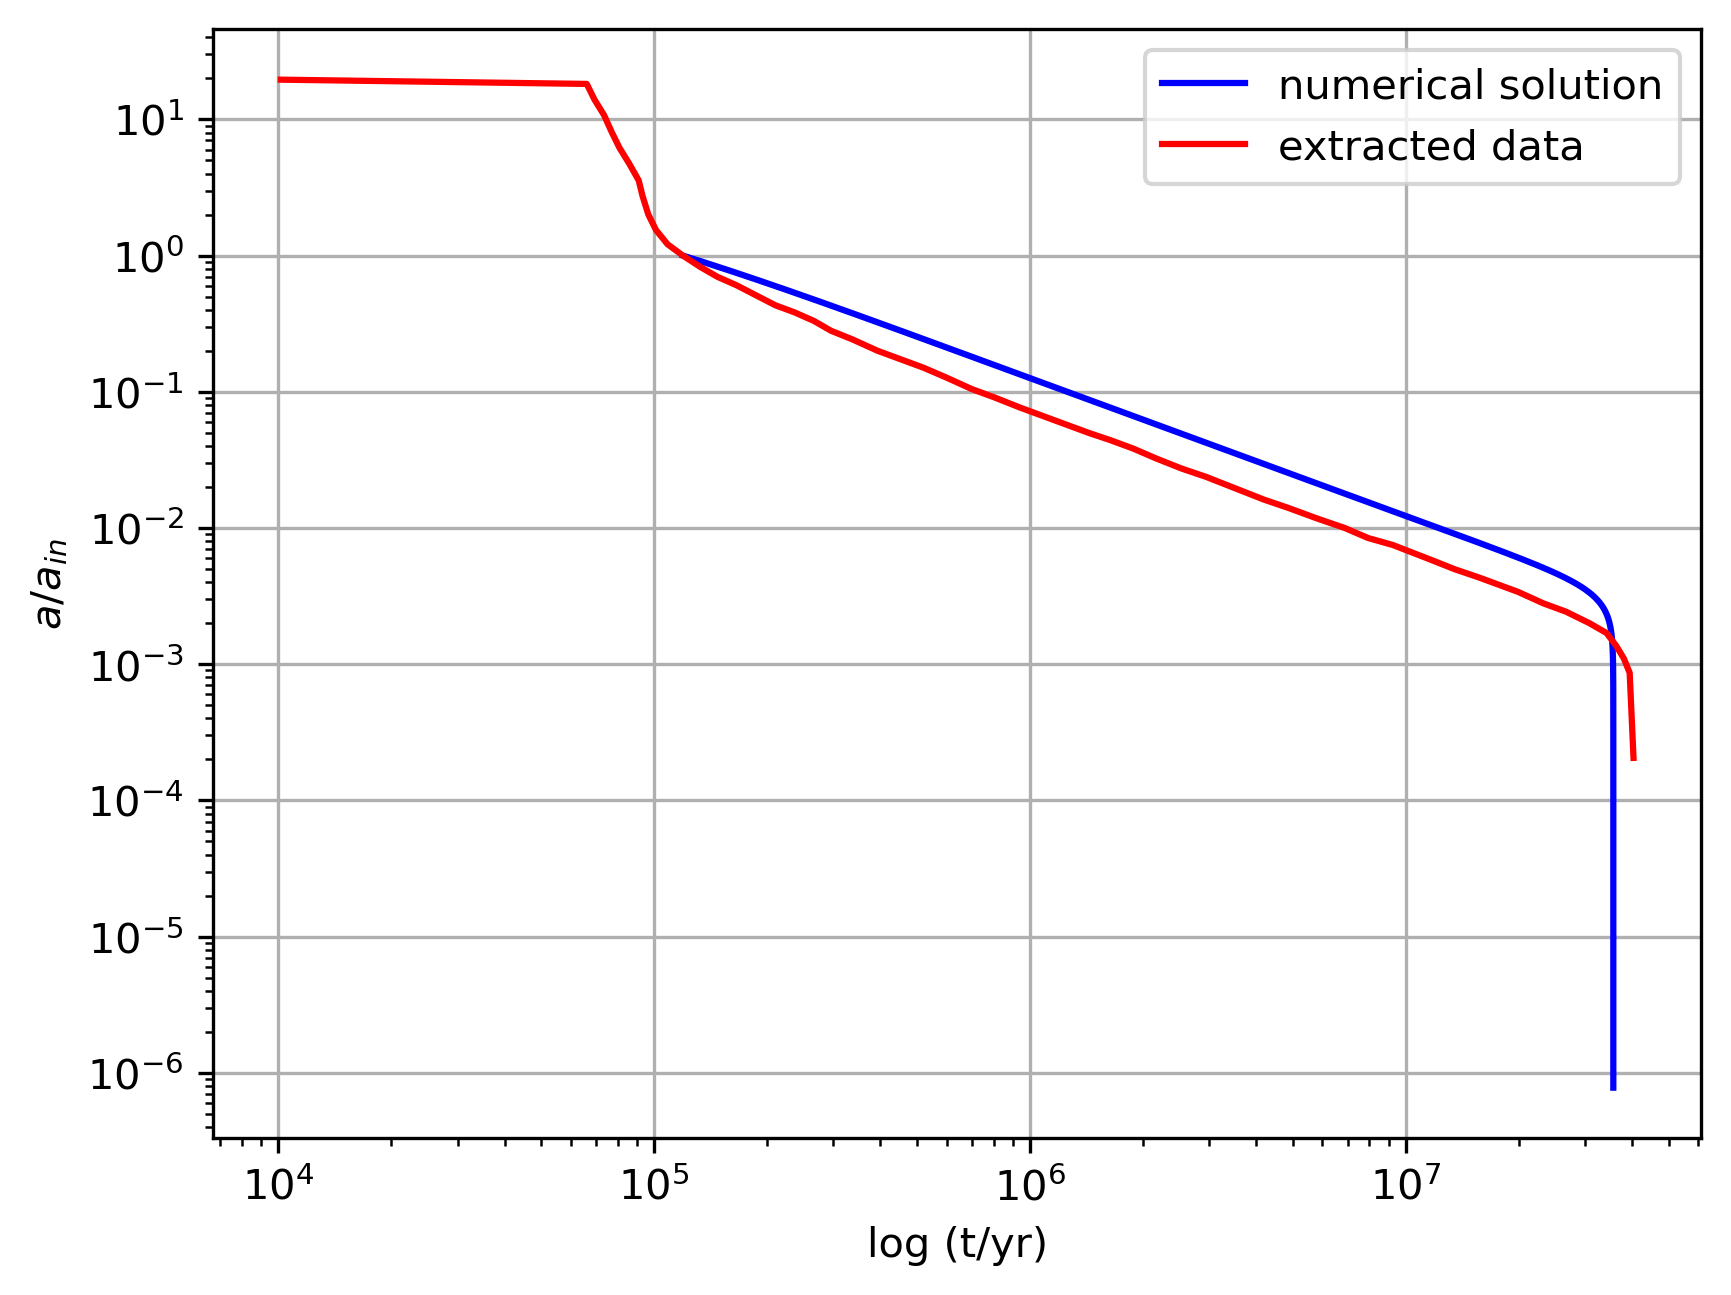
\includegraphics[width=0.5\linewidth]{a_vs_t_check.png}
    \caption{}
    \label{a vs t Sesana comparison}
\end{figure}



\begin{figure}[H]
    \centering
    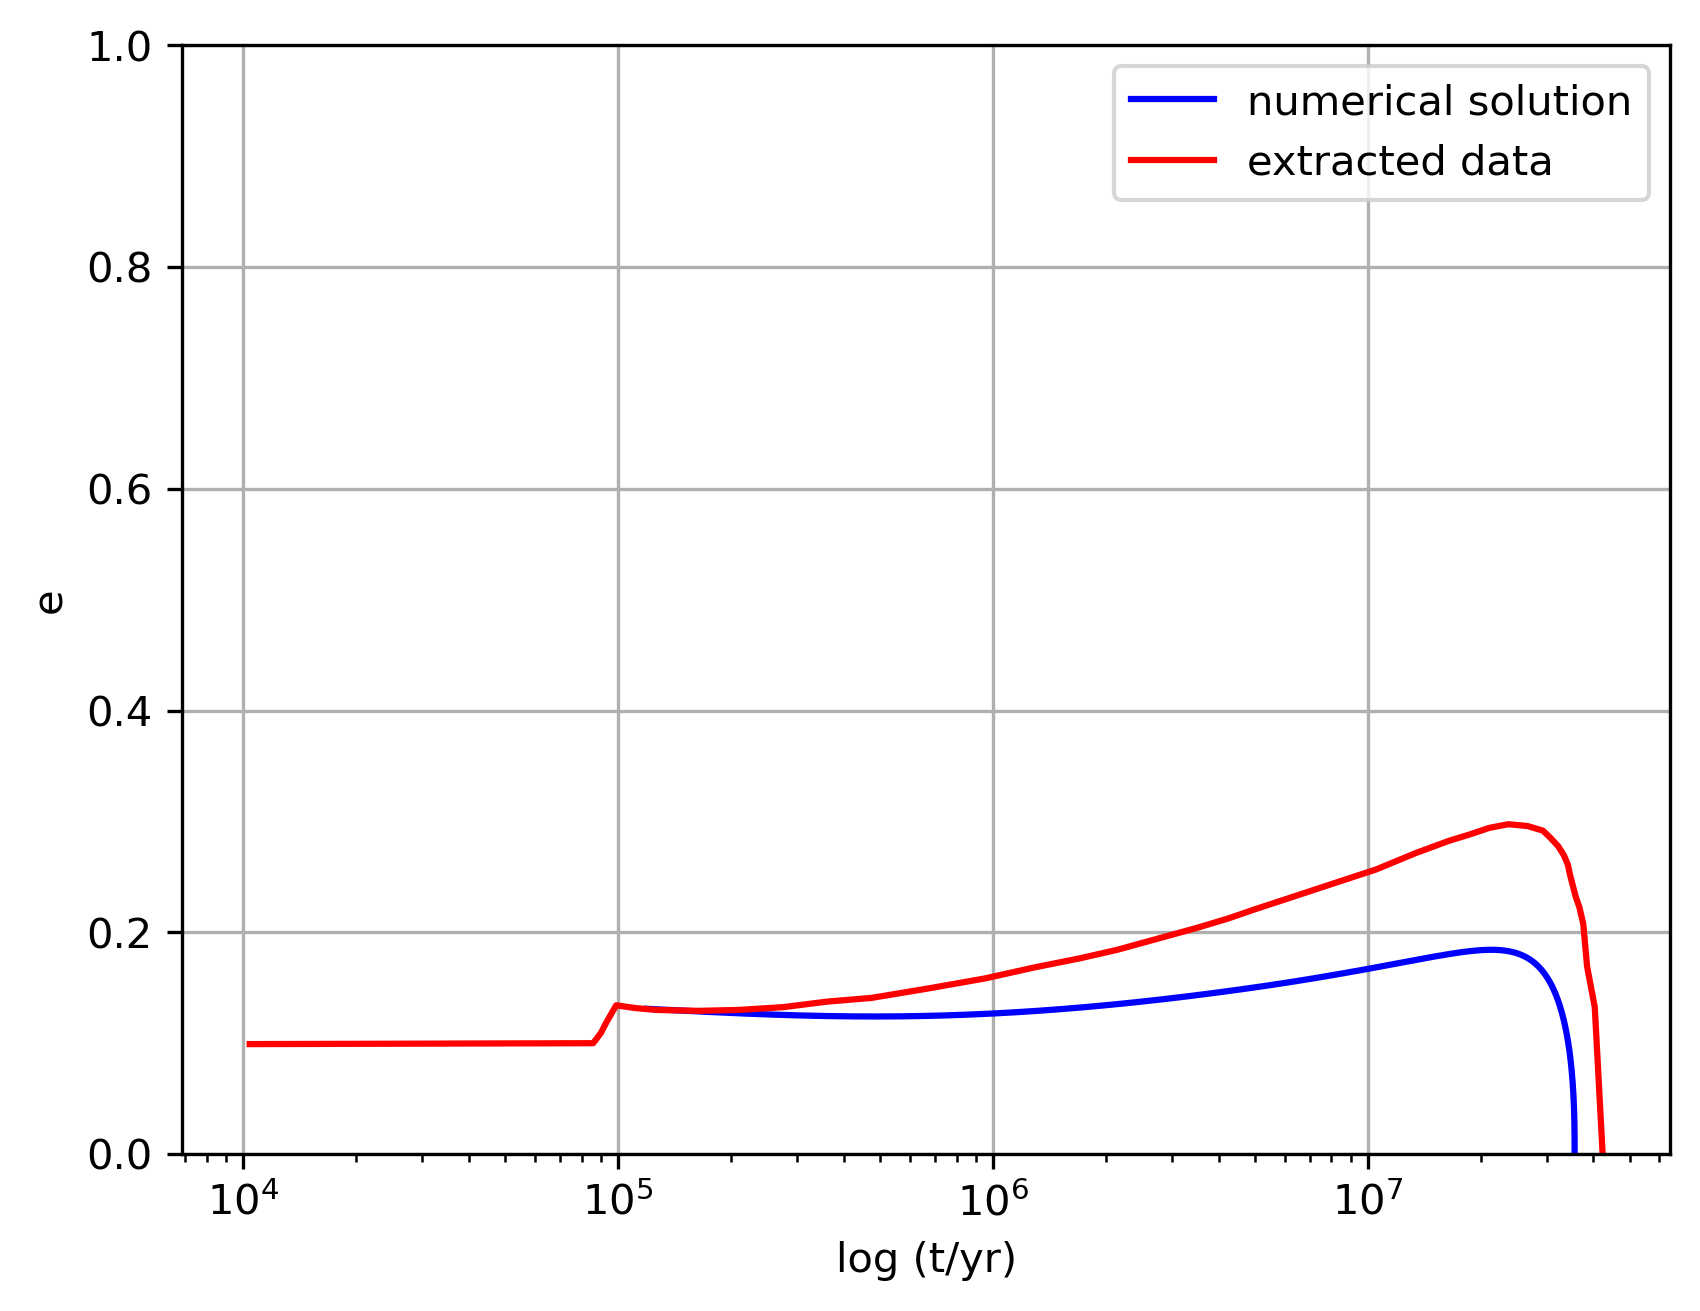
\includegraphics[width=0.5\linewidth]{e_vs_t_check.png}
    \caption{}
    \label{e vs t Sesana comparison}
\end{figure}

Figure \ref{a vs t Sesana comparison} and \ref{e vs t Sesana comparison} indicate a good agreement between our model and Sesana one. In the first plot $a$ decreases more slowly than Sesana prediction as we are negletting the bound cusp erosion contribute, which hardens the binary even when the unbond phase takes over at $\sim a_h$. On the other hand eccentricity reaches a lower peak compared to the reference model because of bound cusp erosion leads to $e$ growth as well.\\Furthermore, we test the feedback of the various shrinking mechanisms by assuming them working in isoletion, hence suppressing all the others.

Figure \ref{a_vs_t_UN} and \ref{e_vs_t_UN} refers to the evolution under the effect of slinghot of unbound stars; as the initial separation is below $a_h$ we can appreciate the expected linear decay of $a$ and the overall eccentricity growth. 
\begin{figure}[H]
    \centering
  \begin{minipage}[c]{0.45\textwidth}
    \centering
    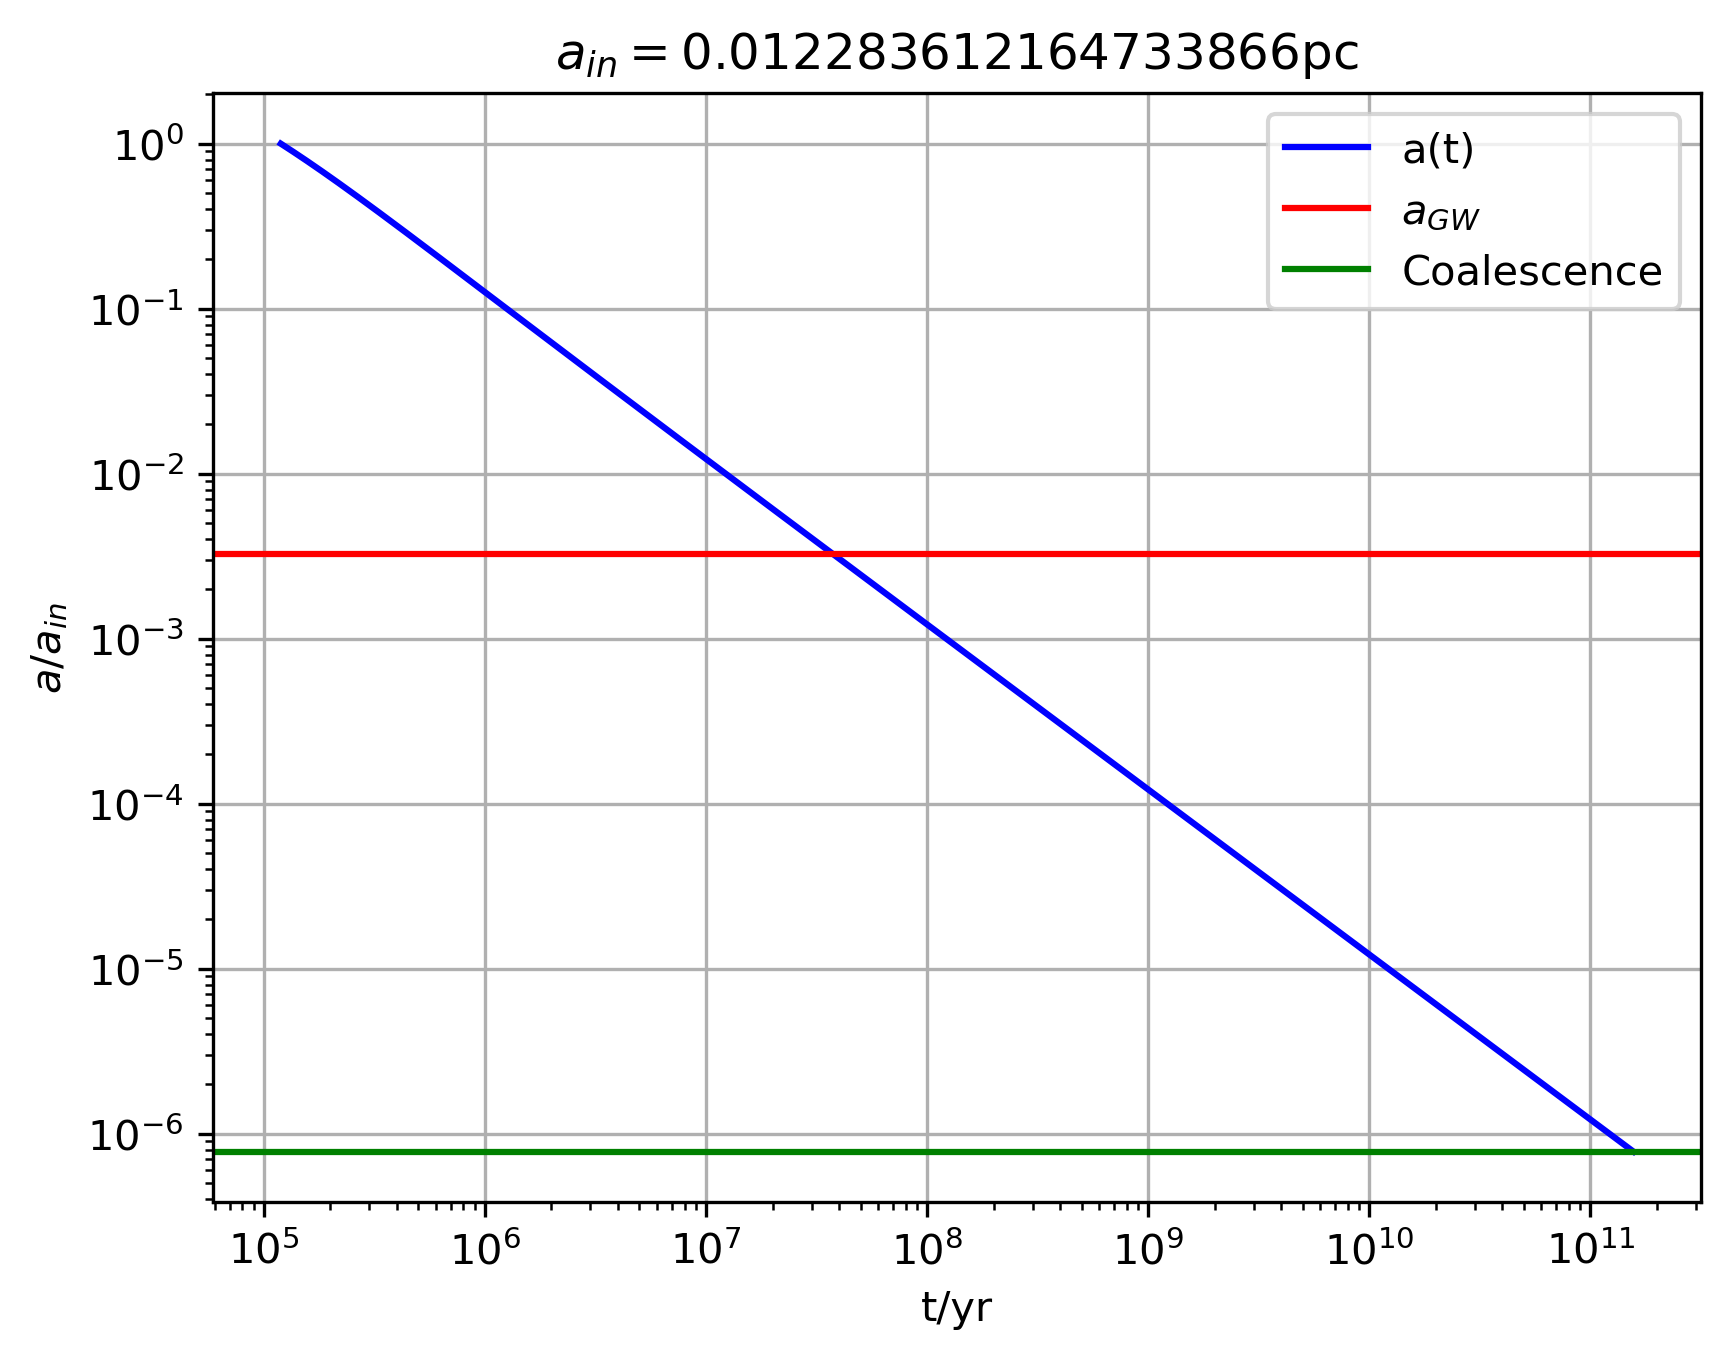
\includegraphics[height=5cm]{a_vs_t_UN.png}
    \caption{}
    \label{a_vs_t_UN}
    \vspace{2mm}
  \end{minipage}
  \hfill
  \begin{minipage}[c]{0.45\textwidth}
    \centering
    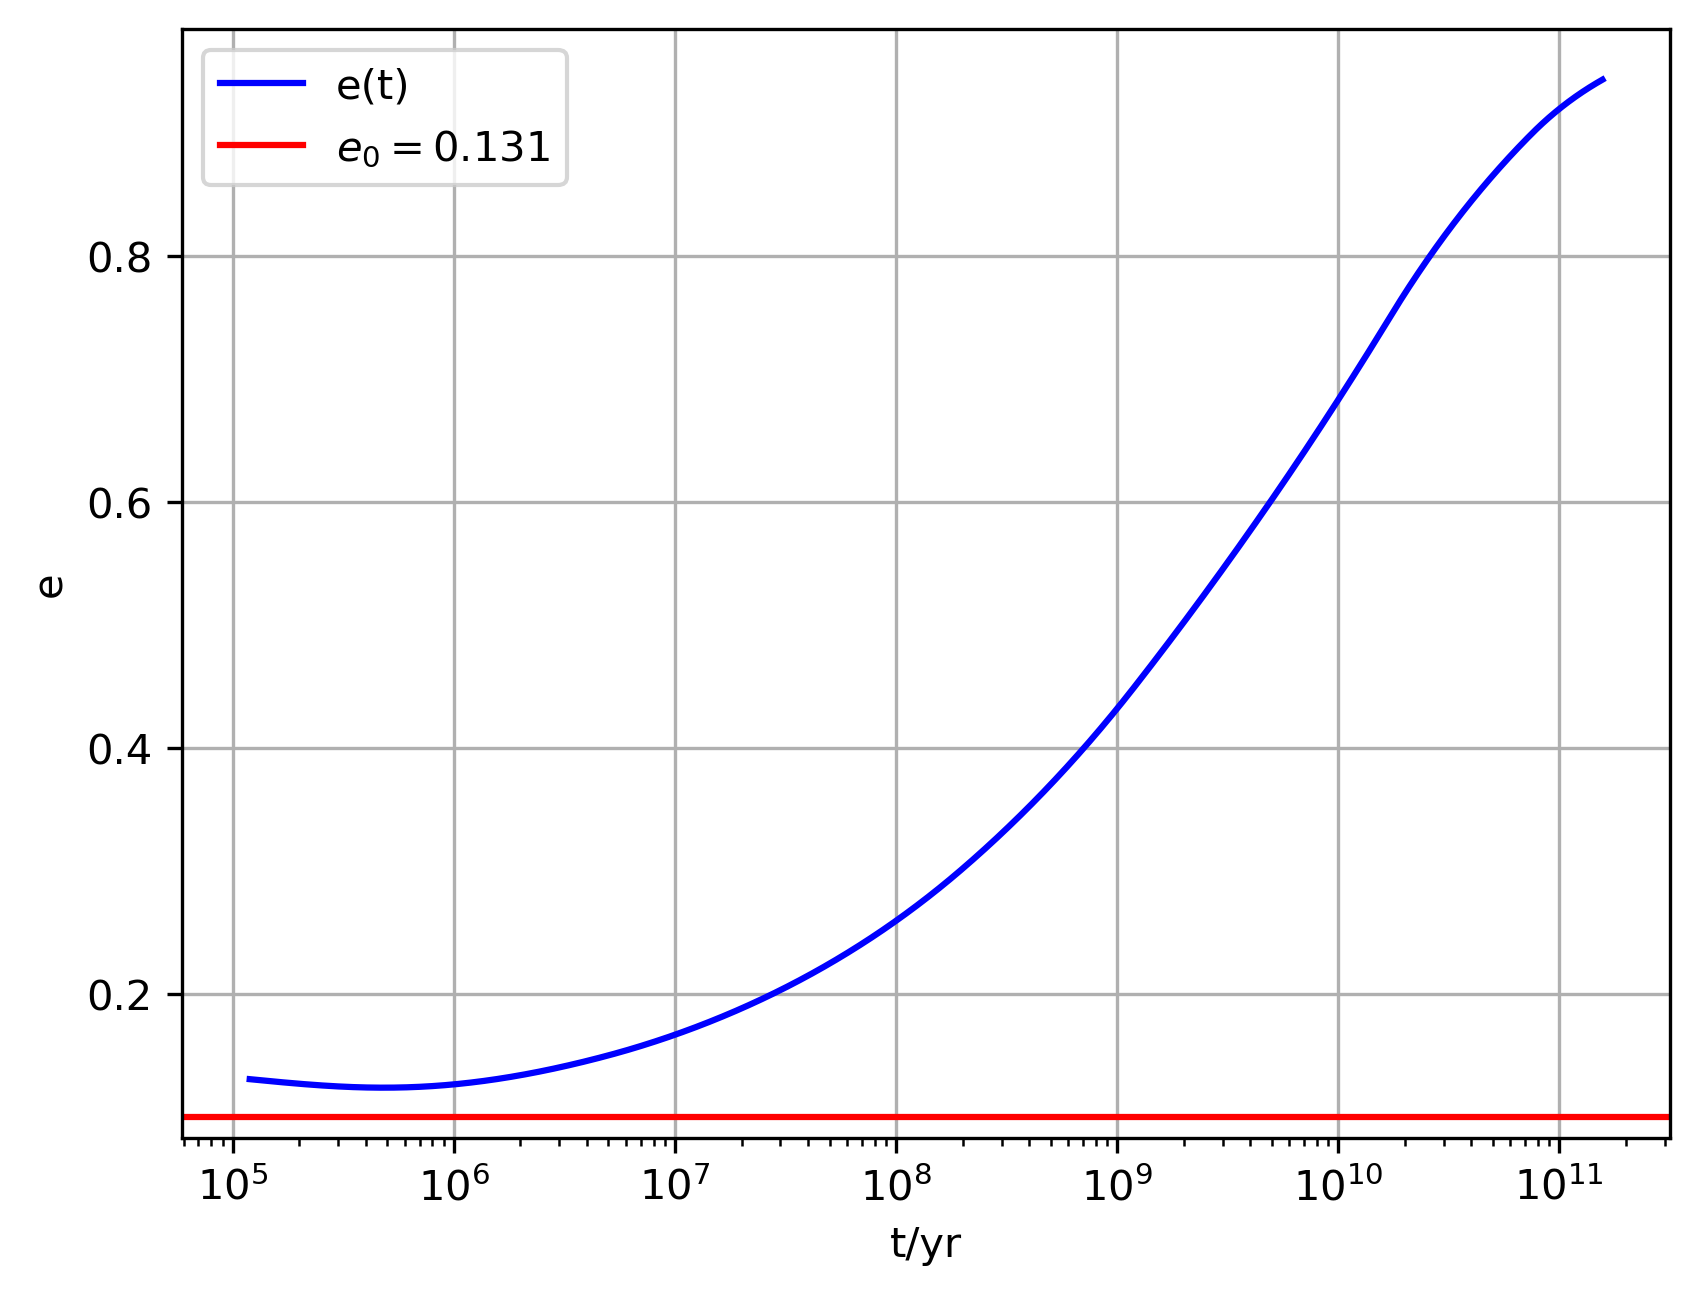
\includegraphics[height=5cm]{e_vs_t_UN.png}
    \caption{}
    \label{e_vs_t_UN}
    \vspace{2mm}
  \end{minipage}
\end{figure}



Figure \ref{a_vs_t_GW} and \ref{e_vs_t_GW} refers to the evolution under GWs production; this becomes effective only at very close separation and causes both the fast binary coalescence once effective and binary circularization. The coalescence time agrees perfectly to the theoretical prediction of Equation \ref{t_coal Maggiore} 




\begin{figure}[H]
    \centering
  \begin{minipage}[c]{0.45\textwidth}
    \centering
    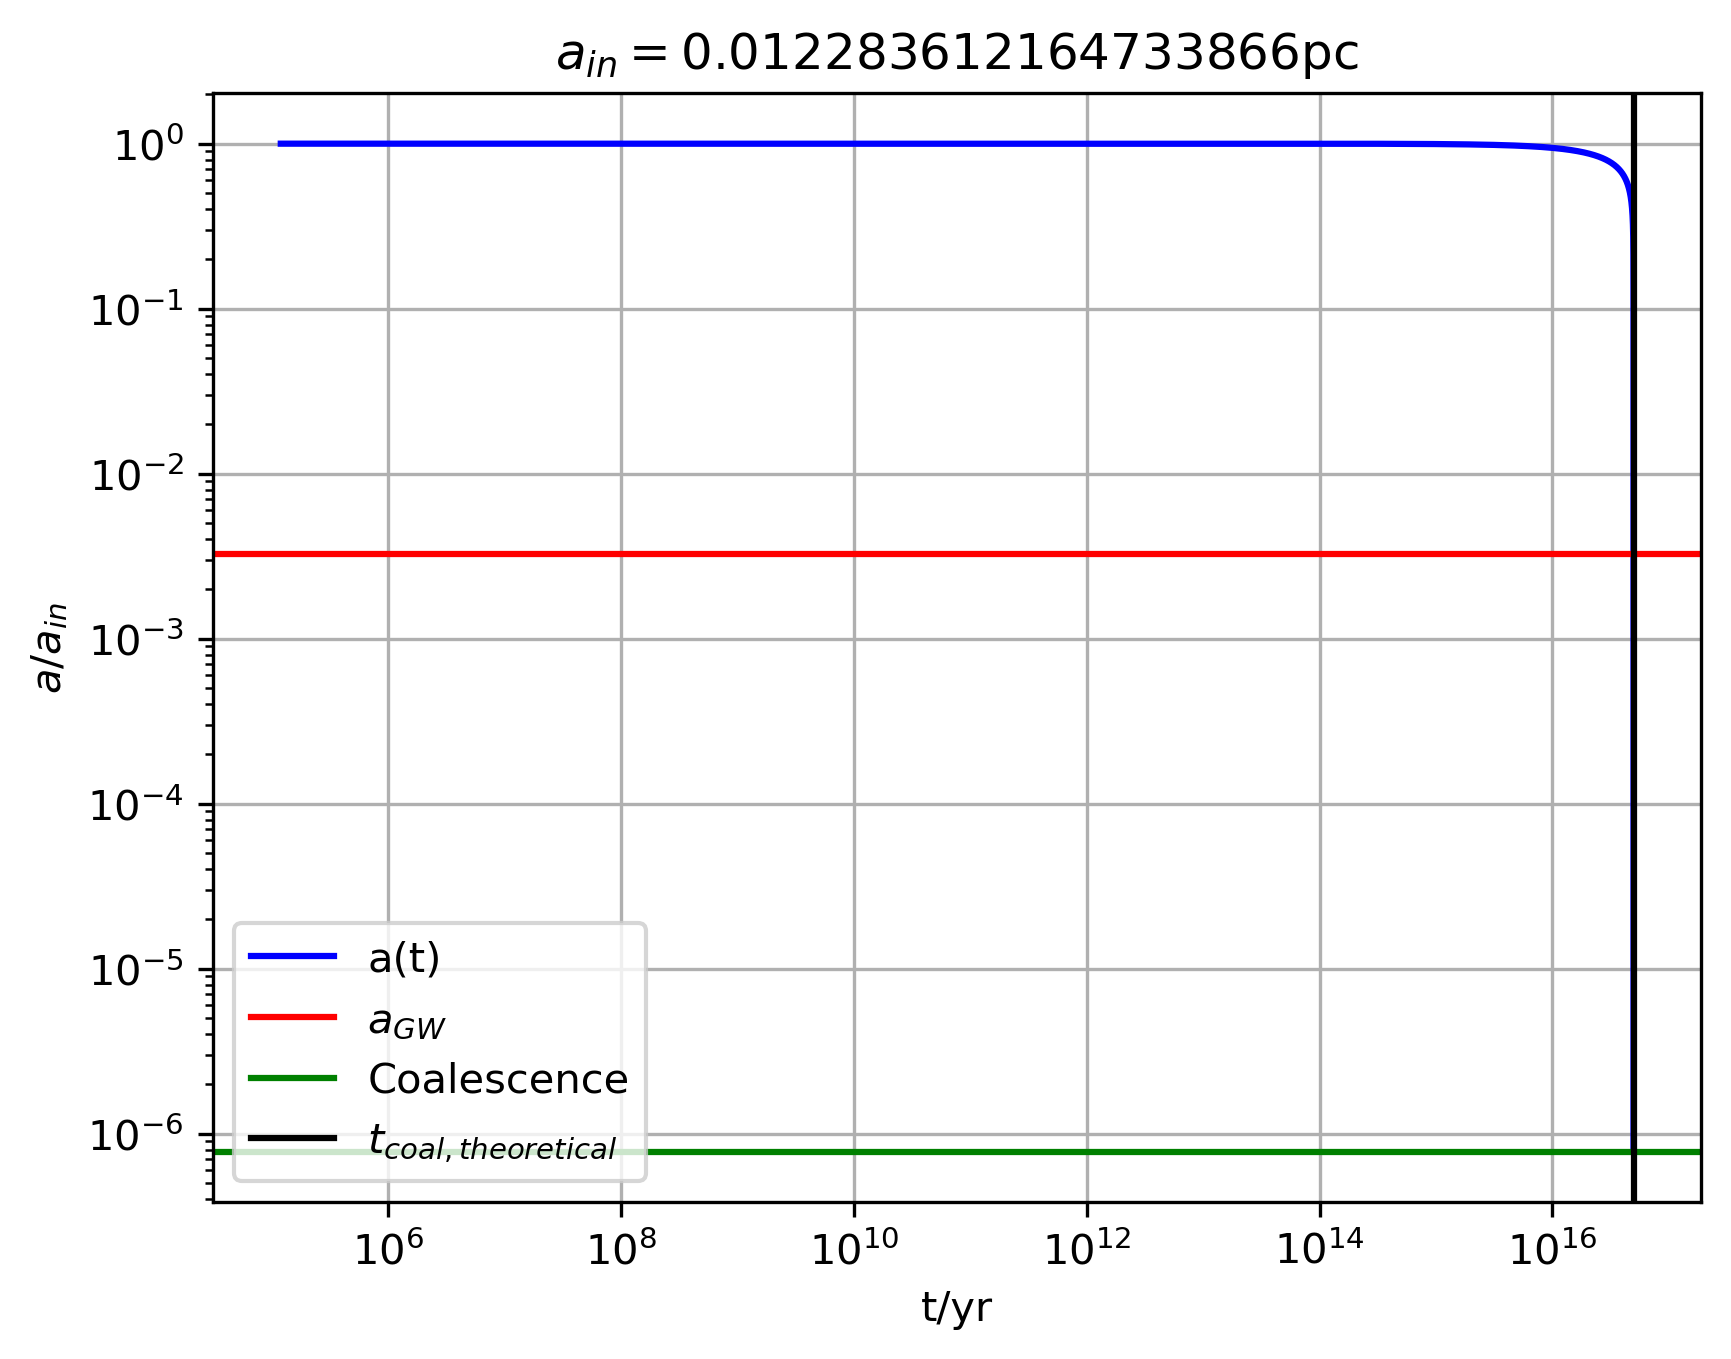
\includegraphics[height=5cm]{a_vs_t_GW.png}
    \caption{}
    \label{a_vs_t_GW}
    \vspace{2mm}
  \end{minipage}
  \hfill
  \begin{minipage}[c]{0.45\textwidth}
    \centering
    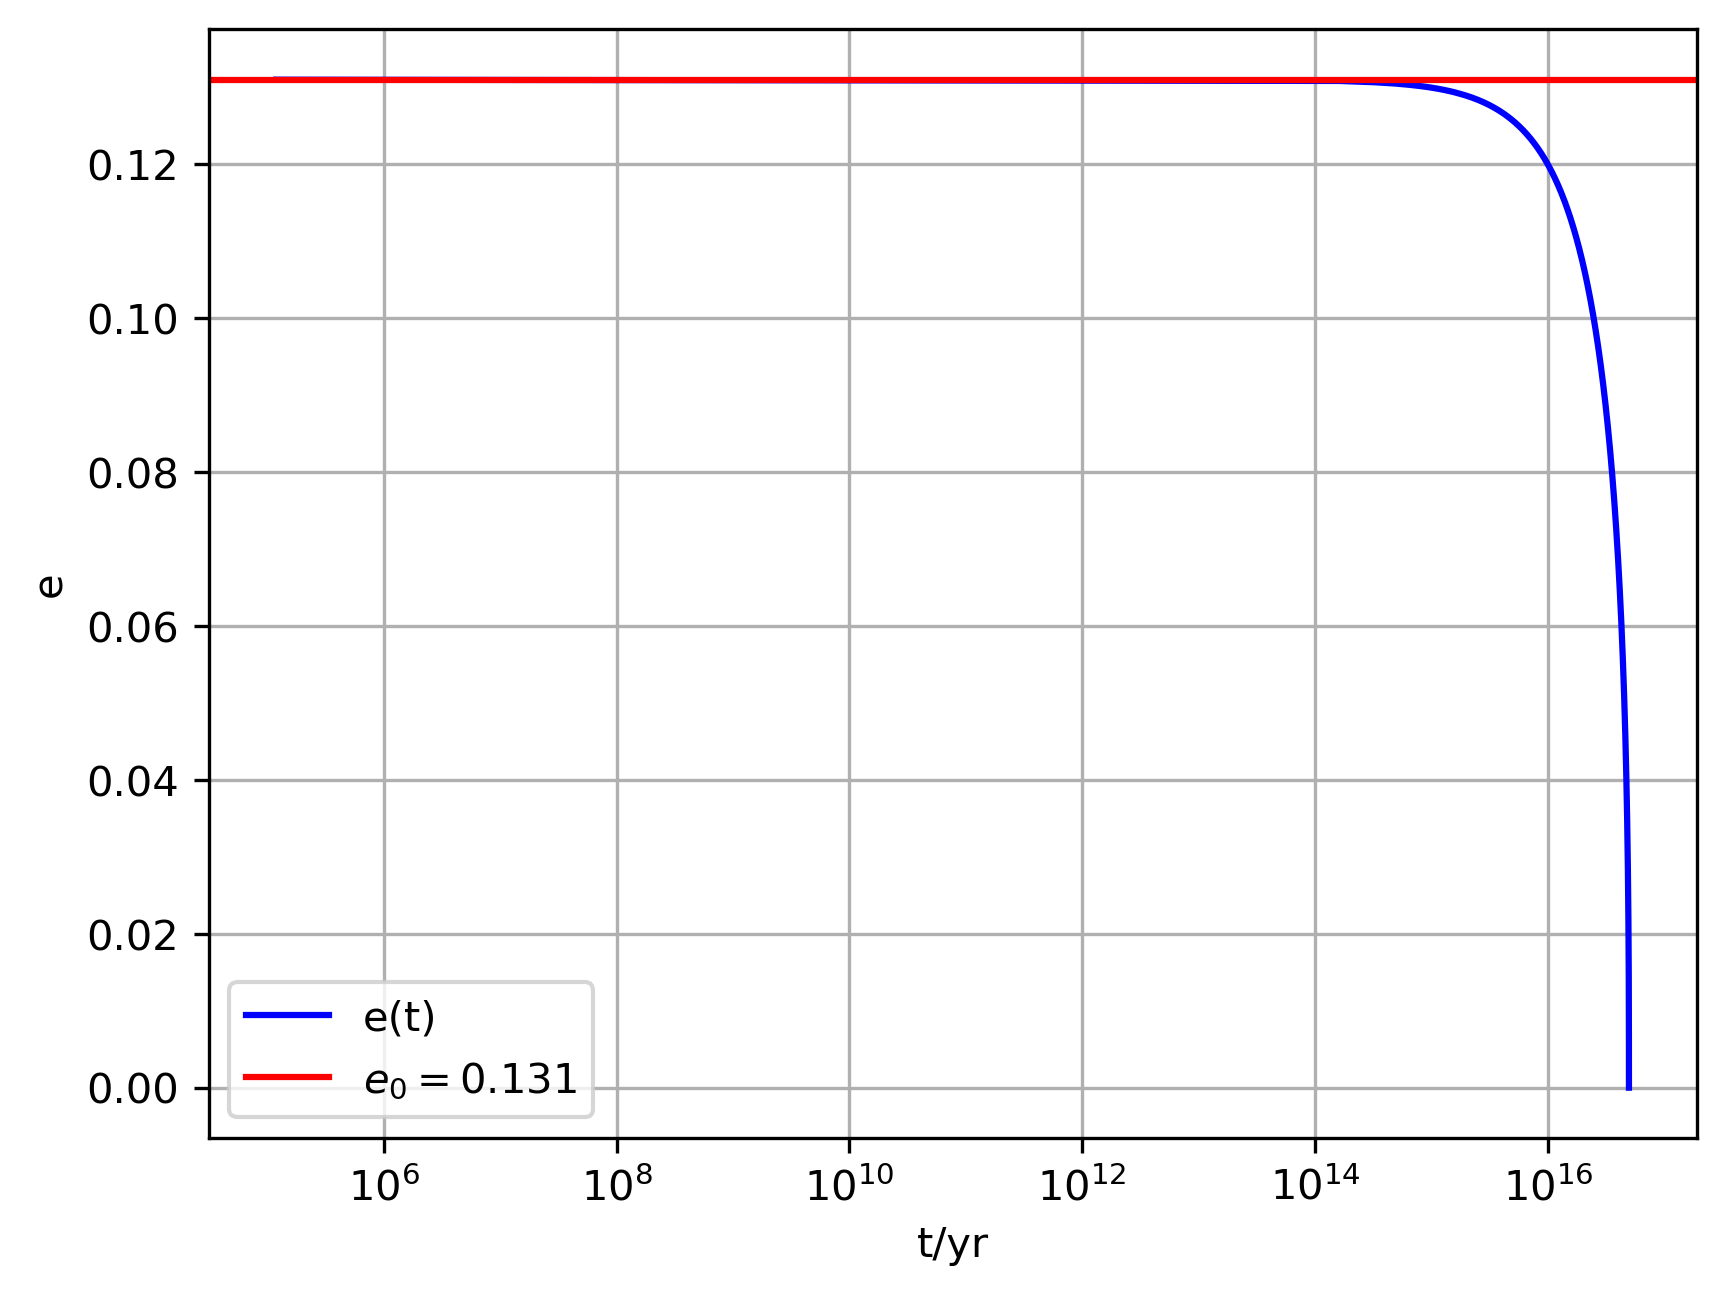
\includegraphics[height=5cm]{e_vs_t_GW.png}
    \caption{}
    \label{e_vs_t_GW}
    \vspace{2mm}
  \end{minipage}
\end{figure}



The dataset used above help us to construct another curve, precisely $(e(t,a(t)))$ which can be compared to the close form solution provided by Equation (\ref{a=a(e) Maggiore}) as shown in Figure \ref{a_vs_e_GW} and \ref{a_vs_e_Maggiore}.




\begin{figure}[H]
    \centering
  \begin{minipage}[c]{0.45\textwidth}
    \centering
    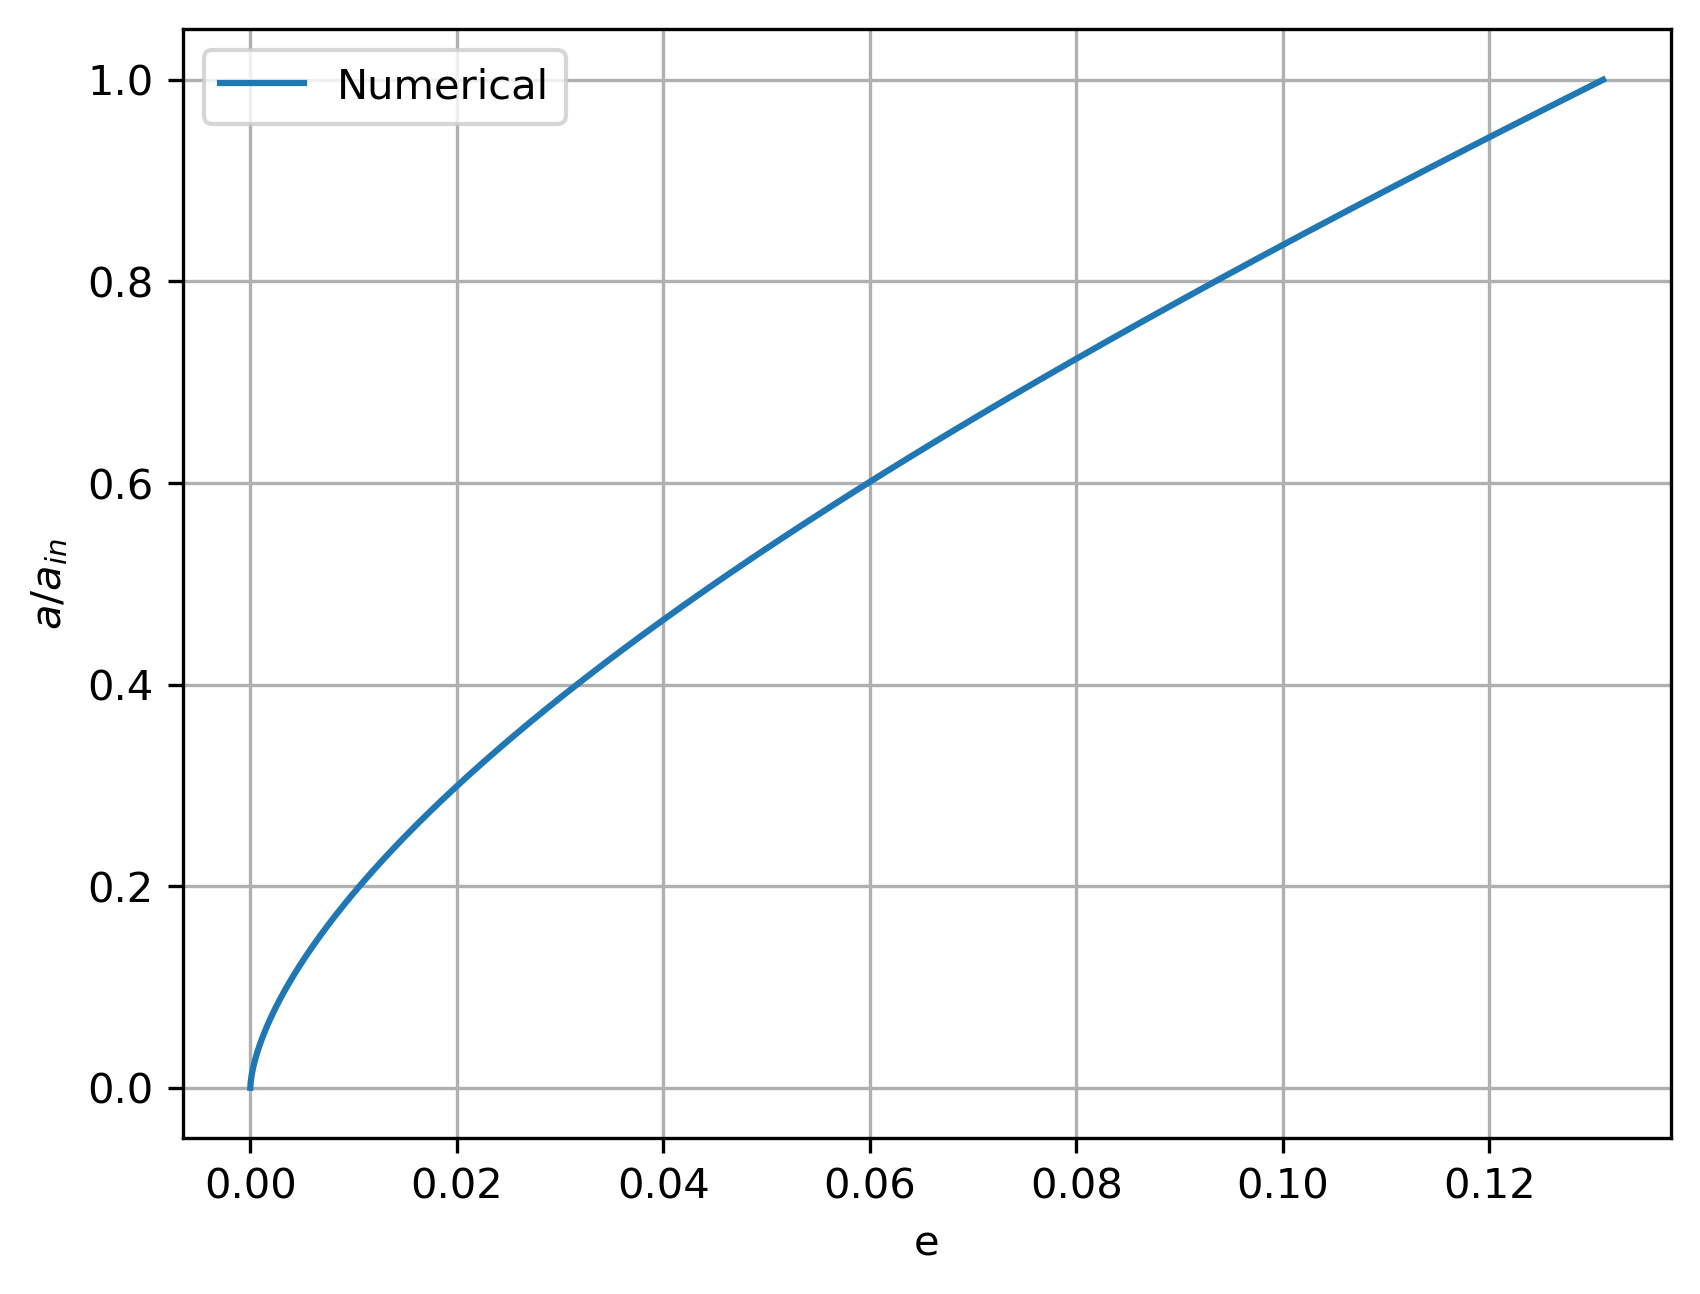
\includegraphics[height=5cm]{a_vs_e_GW.png}
    \caption{}
    \label{a_vs_e_GW}
    \vspace{2mm}
  \end{minipage}
  \hfill
  \begin{minipage}[c]{0.45\textwidth}
    \centering
    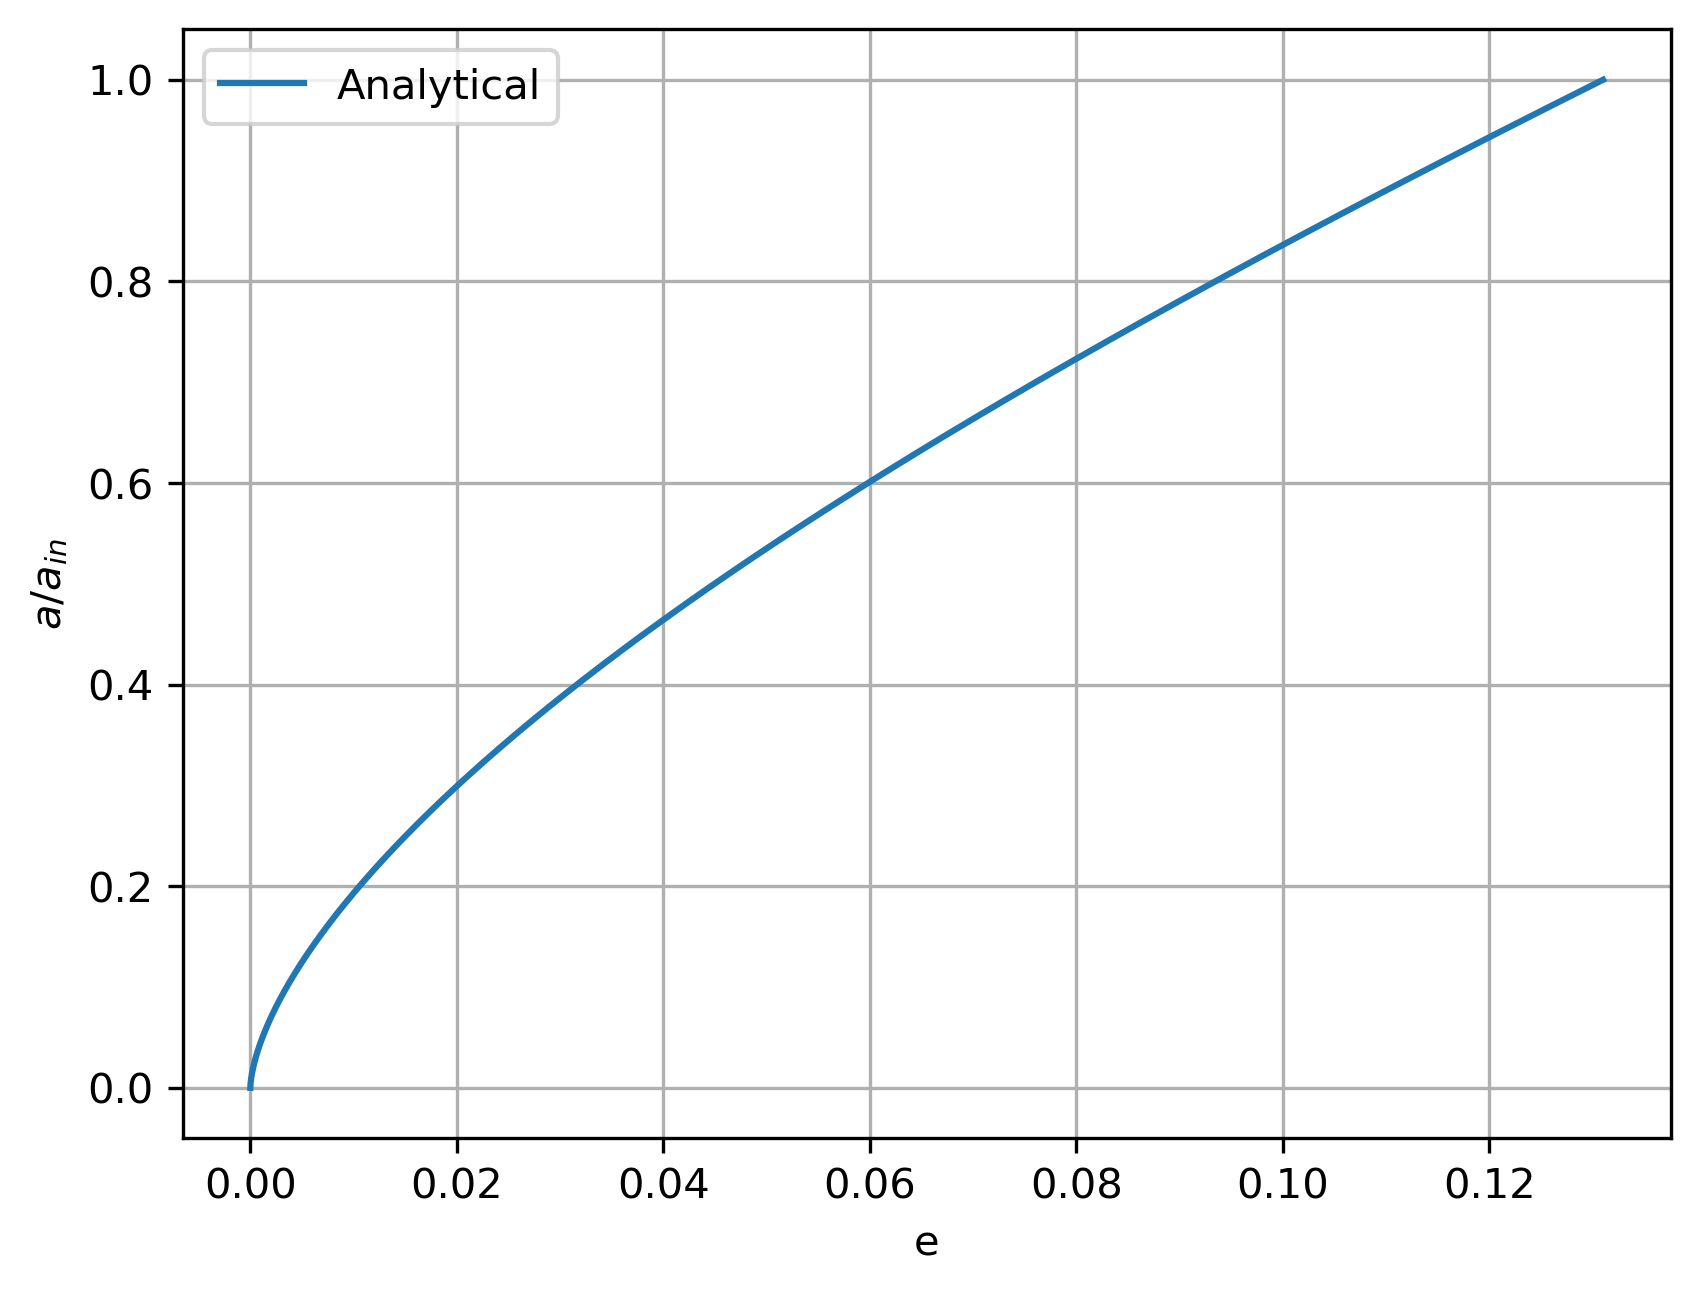
\includegraphics[height=5cm]{a_vs_e_Maggiore.png}
    \caption{}
    \label{a_vs_e_Maggiore}
    \vspace{2mm}
  \end{minipage}
\end{figure}


Below, the Figure \ref{error_a_vs_e_GW} gives us the possibility of visualizing the relative error of the numerical solution with respect to the analytical one; it turnsout to be within one part over $10^{12}$.


\begin{figure}[H]
    \centering
    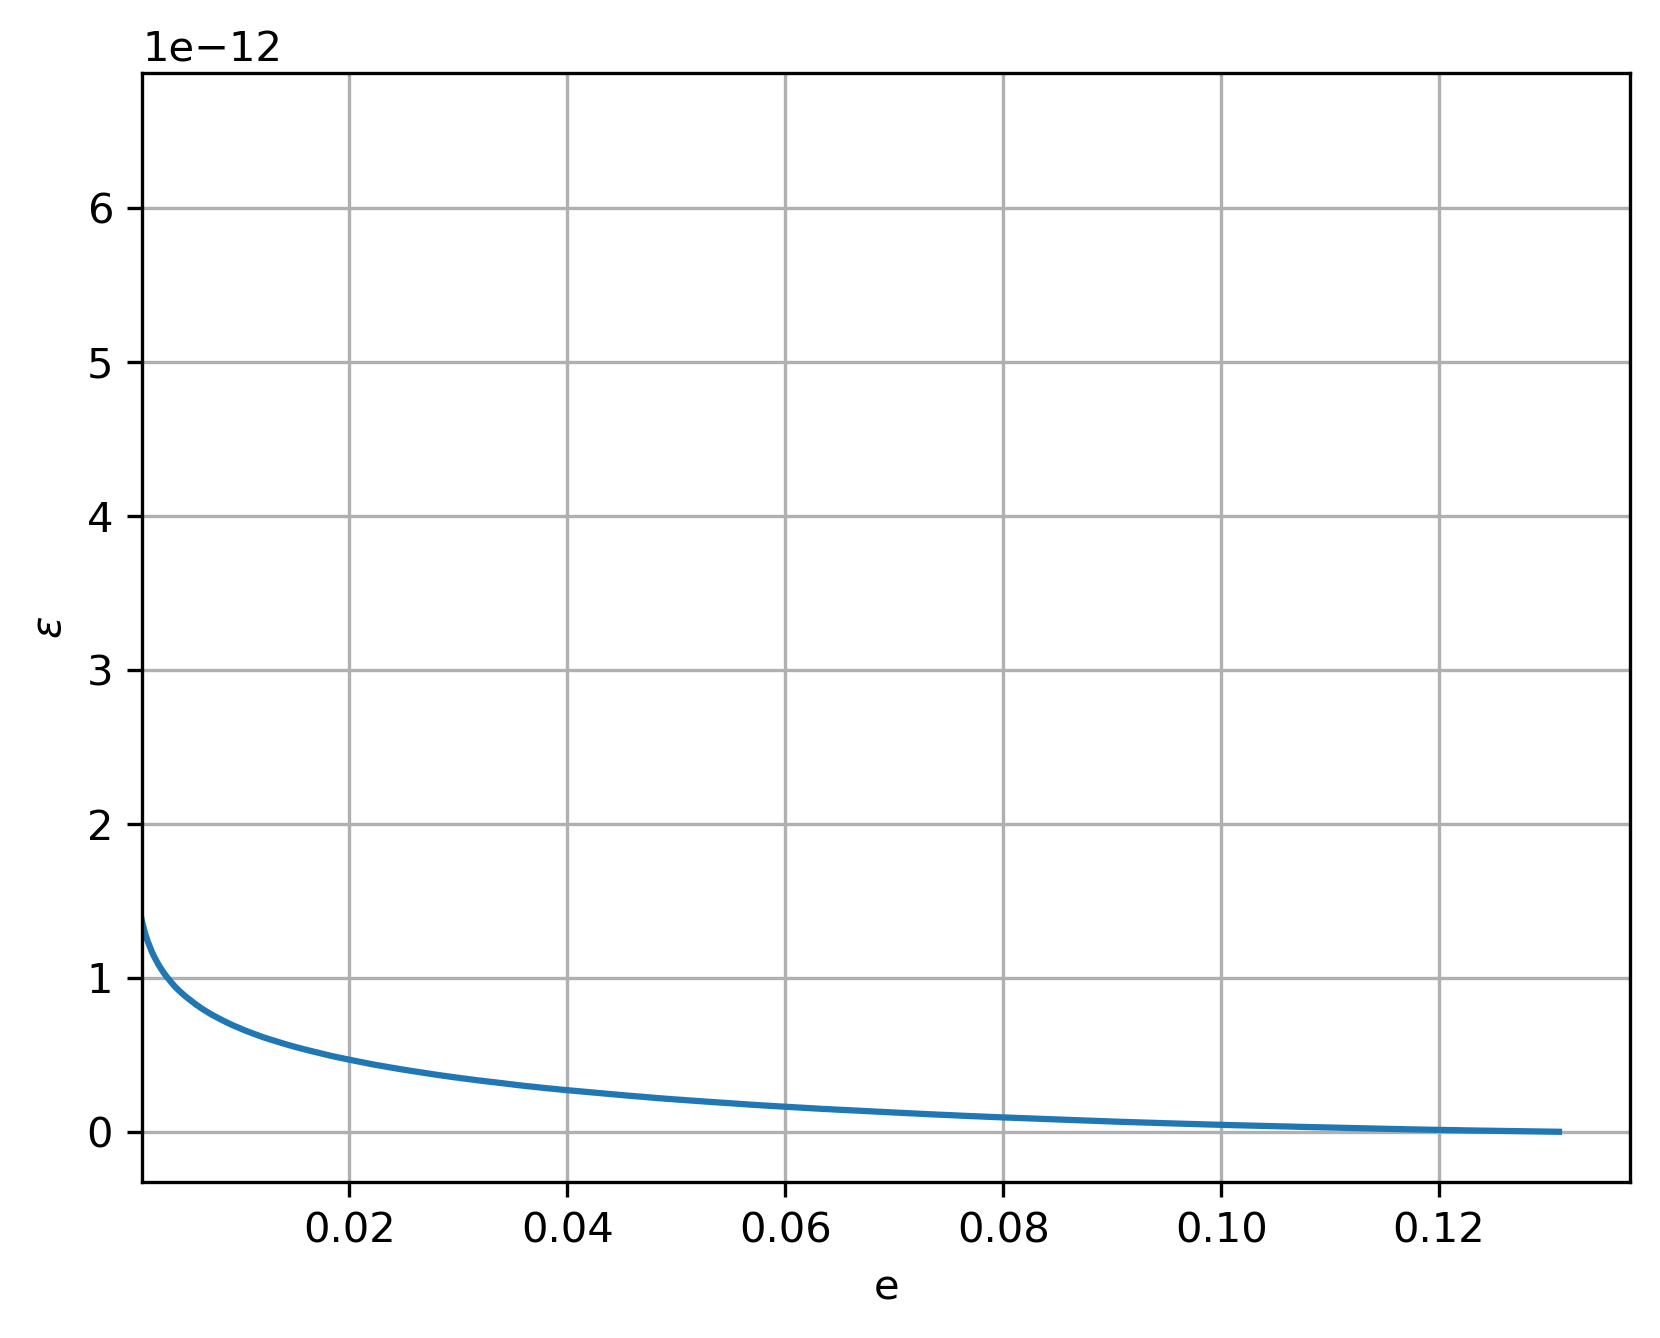
\includegraphics[width=0.5\linewidth]{error_a_vs_e_GW.png}
    \caption{}
    \label{error_a_vs_e_GW}
\end{figure}





%\include{Chapter_3}





\section{NGC 205 IMBH Binary evolution}

\subsection{NGC 205 Hybrid Model Evolution}
NGC 205 is a nearby dwarf galaxy with a NSC residing at its innermost region; it is belived to host an IMBH binary, whose estimated mass is $\sim 10^4 M_\odot$.\\The 2-D surface brightness profile of the dwarf, both the bulge and NSC treated as indipendent stellar components, is translated into 3-D Sersic density profile using Prugniel \& Simien \cite{Prugniel}:

\begin{equation}\label{Prugniel Sersic profile}
    \rho(r)=\rho_0\left(\frac{r}{R_e}\right)^{-p}e^{-b\left(\frac{r}{R_e}\right)^{1/n}}.
\end{equation}
Here, $\rho_0$ is the density normalization unambiguously set by total galaxy mass, effective radius and Sersic index $n$; from \cite{Terzic}:
\begin{equation}
\rho_0
=
\frac{M_*}{4\pi R_e^3}
\frac{b^{\,n(3-p)}}{n\,\Gamma\!\left[n(3-p)\right]}.
\end{equation}
The parameters $p$ and $b$ can be expressed as a function of $n$ as follows: $p=1.0-0.6097/n+0.05563/n^2$, and $b \approx 2 n - 1/3 + 0.009876/n$, for $0.5 < n < 10$.\\Observations constrain the quantites $(M,R_{eff},n)$ for both bulge and NSC as reported in Figure (\ref{Khan_2021_NGC205}) of \cite{Khan_2021}.
\begin{figure}[H]
    \centering
    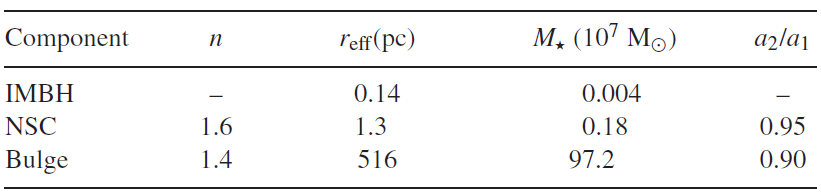
\includegraphics[width=0.5\linewidth]{Khan_2021_table.png}
    \caption{Column 1: Galaxy component. Column 2: Sersic index. Column 3:
Effective radius of the galaxy component (note: for the IMBH, we quote the
influence radius instead). Column 4: Stellar mass. Column 5: 2D axial ratio
as measured by GALFIT.}
    \label{Khan_2021_NGC205}
\end{figure}
 It has (with standard substitution $Z=b\left(\frac{r}{R_e}\right)^{1/n}$)
\begin{equation}\label{Sersic mass profile}
    M(<r)=4\pi \rho_0 R_e^3 n b^{n(p-3)}\gamma\left[n(3-p),b\left(\frac{r}{R_e}\right)^
    {1/n}\right]=M_*\frac{\gamma\left[n(3-p),b\left(\frac{r}{R_e}\right)^
    {1/n}\right]}{\Gamma[n(3-p)]}
\end{equation}
with
\begin{equation}\label{complete gamma fun}
    \Gamma(a)=\int_{0}^{\infty}dt e^{-t}t^{a-1}
\end{equation}
the "Complete gamma function",
\begin{equation}\label{upper incomplete gamma fun}
    \Gamma(a,x)=\int_{x}^{\infty}dt\,e^{-t}t^{a-1}
\end{equation}
the Upper incomplete gamma function and
\begin{equation}\label{lower incomplete gamma fun}
    \gamma(a,x)=\int_{0}^{x}dt\,e^{-t}t^{a-1}
\end{equation}
the Lower incomplete gamma function. By definition follows:
\begin{equation}\label{gamma fun relation}
    \Gamma(a)=\Gamma(a,x)+\gamma(a,x)
\end{equation}
The spatial distribution is spherical and untruncated but the mass profile converges to
the finite value $M_*$, so the potential can be found from
\begin{equation}\label{spherical potential, general formula}
    \Phi(r)=\Phi(r_0)+\frac{GM(<r_0)}{r_0}-\frac{GM(<r)}{r}-4\pi G \int_{r}^{r_0}dt\,t \rho(t)
\end{equation}
Setting $r_0\rightarrow \infty$ and $\Phi(r_0)=0$, it becomes
\begin{equation}\label{spherical potential, simplified formula}
    \Phi(r)=-\frac{GM(<r)}{r}-4\pi G \int_{r}^{\infty}dt\,t \rho(t)
\end{equation}
and computation returns
\begin{equation}
\Phi(r)=
-4\pi G \rho_0 R_e^2 n\, b^{\,n(p-2)}
\left\{
\frac{b^{-n}}{r/R_e}\,
\gamma\!\left[n(3-p),Z\right]
+
\Gamma\!\left[n(2-p),Z\right]
\right\}
\end{equation}
or equivalently
\begin{equation}
    \Phi(r)=-\frac{GM_*}{r}\left\{\frac{\gamma\!\left[n(3-p),Z\right]}{\Gamma[n(3-p)]
    }+Z^n\frac{\Gamma[n(2-p),Z]}{\Gamma[n(3-p)]}\right\}
\end{equation}





Numerically it is found
\begin{itemize}
    \item Bulge: $\rho_0=4.80\cdot 10^5M_\odot/pc^3$
    \item NSC: $\rho_0=2.95M_\odot/pc^3$
\end{itemize}
and NGC 205 density profile is reconstructed in  Figure (\ref{NGC205 density profile}).

\begin{figure}[H]
    \centering
    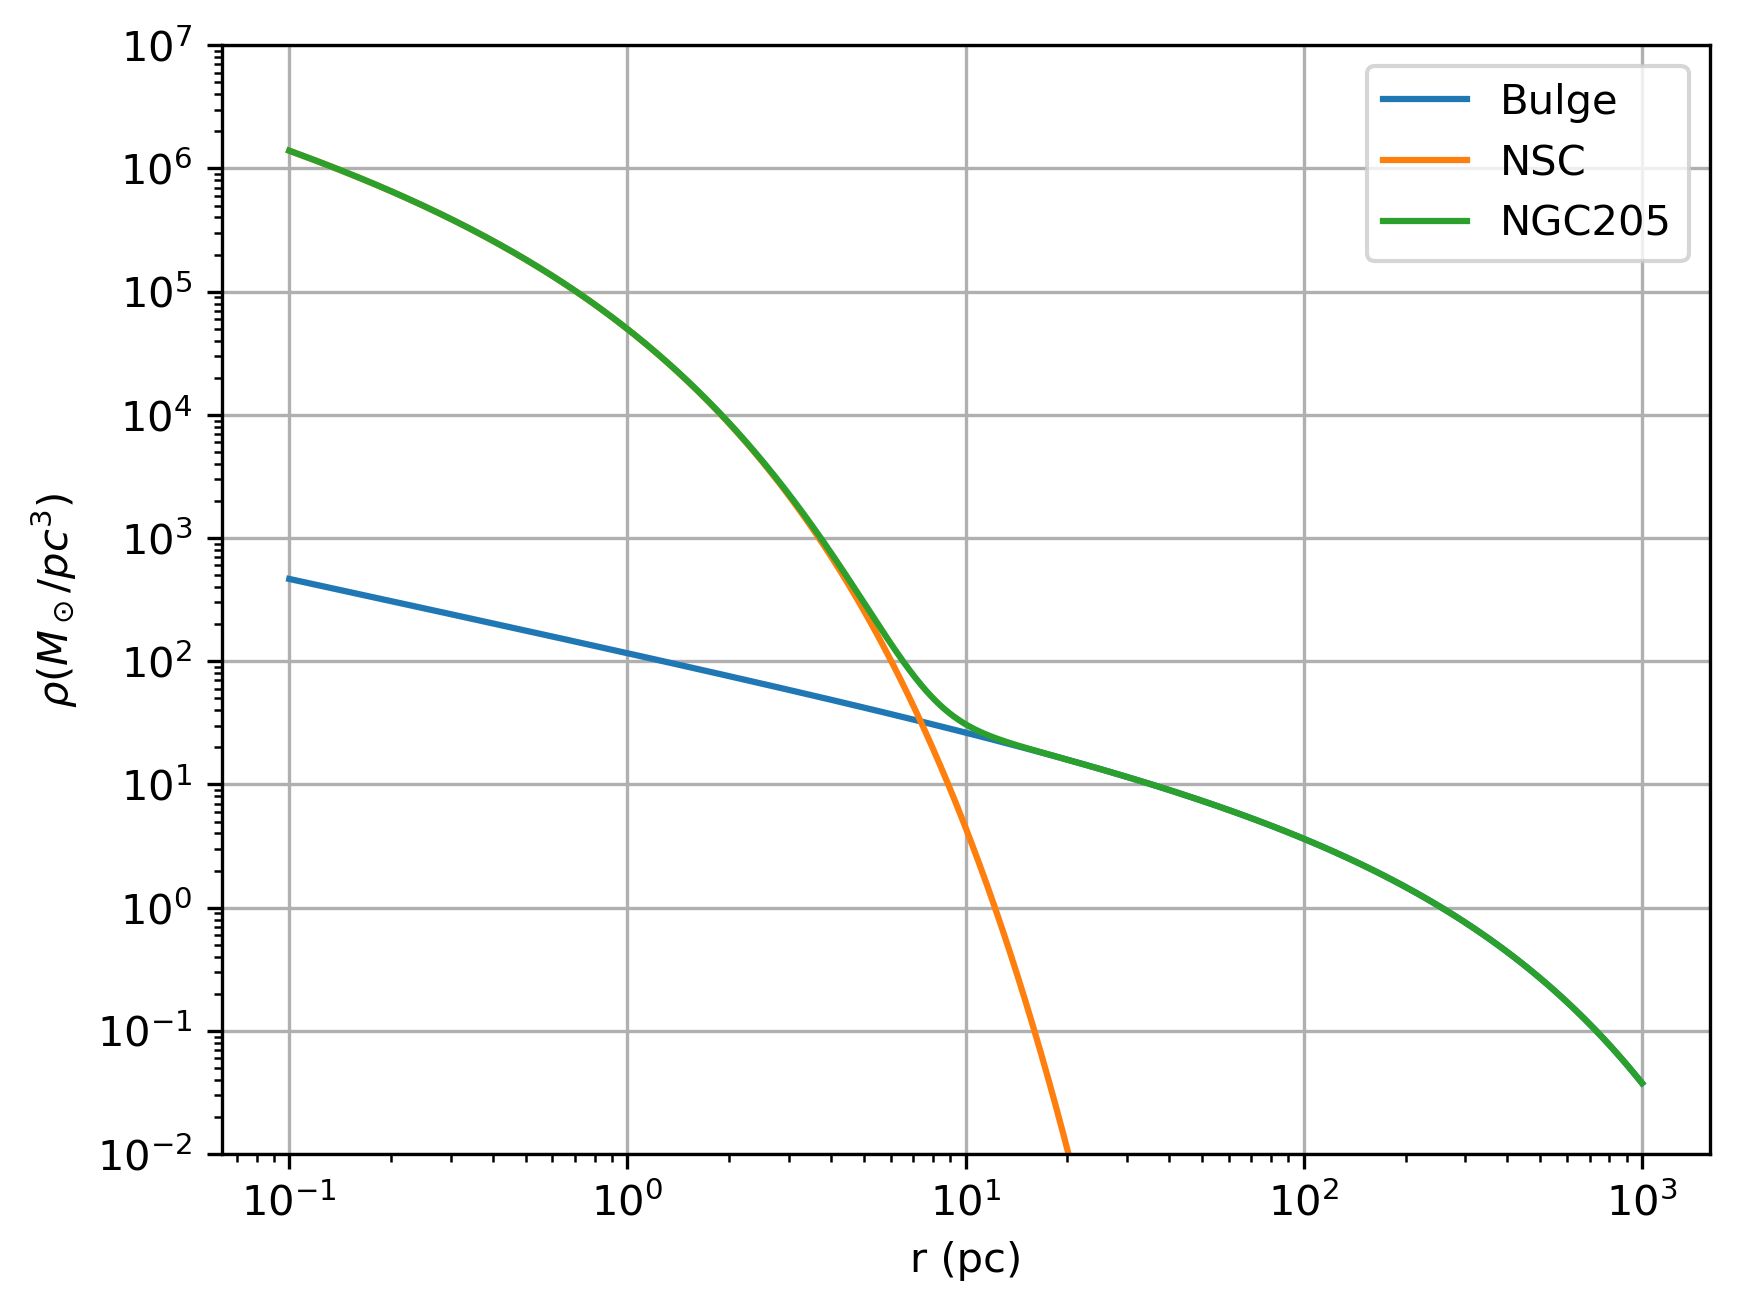
\includegraphics[width=0.5\linewidth]{NGC205_density_profile.png}
    \caption{NGC 205 bulge, NSC and total mass density profile of stellar distribution.}
    \label{NGC205 density profile}
\end{figure}
Adopting the same prescription of \cite{Khan_2021} and \cite{Holley-Bockelmann_2025}, a symmetric IMBH binary of masses $M_1=M_2=4\cdot10^4M_\odot$ is introduced into NGC 205 core and its evolution, due to stellar and GWs hardening, is tracked combining 3-body scattering experiment hybrid model \cite{Quinlan_1996},\cite{Sesana_2006} and \cite{Peters_1963} equations.\\It is quite relevant to point out that in this astrophysical system the hardening due to bound stars \cite{Sesana_2008} is negligible in light of the symmetry of the binary and the arguments exposed at the end of Sec.(\ref{sec:Loss Cone}).\\Therefore, combining the set of equations related to Unbound evolution
\begin{equation}\label{da/dt UNBOUND}
    \frac{da}{dt}|_u = -\frac{a^2 G \rho_{\mathrm{inf}}}{\sigma}  H
\end{equation}

\begin{equation}\label{de/dt UNBOUND}
    \frac{de}{dt}|_u = \frac{a G \rho_{\mathrm{inf}}}{\sigma}  H K
\end{equation}
and the equations describing GWs driven hardening \ref{da/dt Peterson} \ref{de/dt Peterson}, the set of differential equations must be solved reads

\begin{equation}\label{da/dt Un+GW}
    \frac{da}{dt} = \frac{da}{dt}|_u+\frac{da}{dt}|_{gw}
\end{equation}

\begin{equation}\label{de/dt Un+GW}
    \frac{de}{dt} = \frac{de}{dt}|_u+\frac{de}{dt}|_{gw}
\end{equation}
Although the original formulation of the hybrid model relies on a SIS profile, with very peculiar features (i.e. costant velocity dispersion), Sesana \cite{Sesana_2015} showed how to use it for a more general stellar background. The vast majority of stars, unbound to the binary, refilling the loss cone (i.e. having pericenter $\sim a$) come from a region that is just beyond the binary influence radius, hence $r_{inf}$ is the relevant physical scale of the model and $\sigma$ appearing in Equations \ref{da/dt UNBOUND} and \ref{de/dt UNBOUND}, which is in general a function of the radius for spherically symmetric systems, must be computed at the influence radius (here defined as the radius enclosing stellar mass that is twice the binary one).\\Apart from setting the inital point in the $(a,e)$ space, we need to determine several quantities; we start with binary influence radius and $\sigma_{inf}=\sigma(r_{inf})$; they both require the knowledge of the cumulative mass $M(<r)$ associated to the Sersic profile. It results from the integration of $\rho(r)$ and admits analytic solution \cite{Terzic}
\begin{equation}
M(<R)
=
M_{\rm tot}\,
\frac{
\gamma\!\left(
2n,\;
b_n \left(\frac{R}{R_e}\right)^{1/n}
\right)
}{
\Gamma(2n)
}.
\end{equation}
The root of the equation
\begin{equation}
    M(<r_{inf})-2(M_1+M_2)=0
\end{equation}
is obtained numerically by bisection and holds $r_{inf}=0.47pc$.\\On the other hand, Jeans equation provides a way to compute the velocity dispersion and in case of spherical distributions it greatly simpifies to
\begin{equation}\label{Jeans velocity dispersion equation}
\sigma^2(r) =
\frac{1}{\rho(r)}
\int_r^\infty
\rho(s)\,\frac{G M(<s)}{s^2}
ds.
\end{equation}
The integral leads to $\sigma_{inf}=$32.6km/s.
As both $\sigma(r)$ and the circular speed $V_c(r)=\sqrt{GM(<r)/r}$ depend on $M(<r)$, previously obtained, we can derive them and Figure \ref{sigma/Vc NGC205} displays their ratio as afunction of the radius.  


\begin{figure}[H]
    \centering
    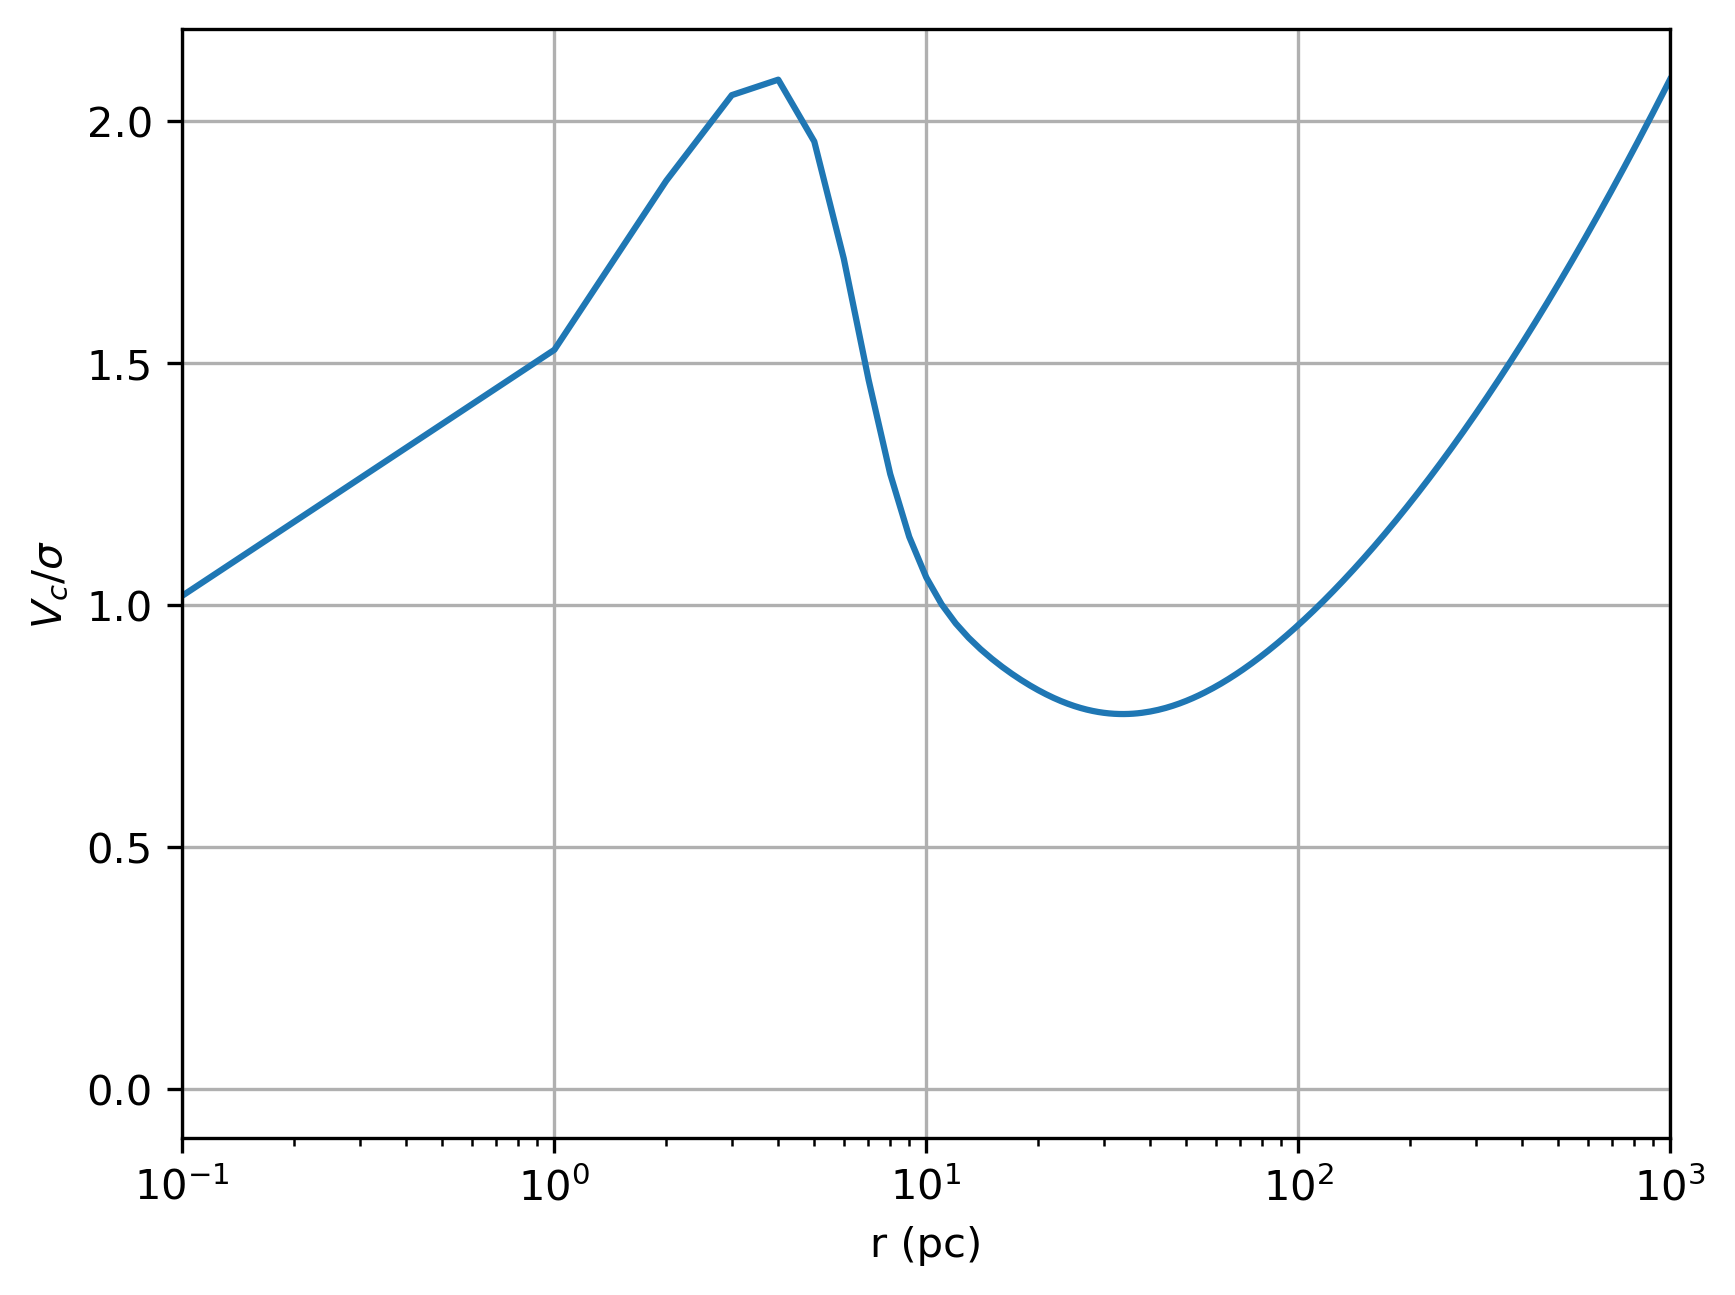
\includegraphics[width=0.5\linewidth]{NGC205_Vc_over_sigma_profile.png}
    \caption{NGC 205 $V_c/\sigma$ vs r}
    \label{sigma/Vc NGC205}
\end{figure}

The last quantity we have to specify in order to implement the hybrid model is the binary hardening radius $a_h$; indeed Sesana \cite{Sesana_2006} found out from 3-body scattering experiments that $H$ and $K$ functions can be fitted to
 \begin{equation}
     H=A(1+a/a_0)^\gamma
\end{equation}
and
 \begin{equation}
    K=A(1+a/a_0)^\gamma+B
\end{equation}
The parameters of the fits to H and J are listed in Tables 1 and 2 of \cite{Sesana_2006} for different binary mass ratios and eccentricity; there, $a_0$ is given in $a_h$ units, thus forcing us to determine it. In literature several definitions have been proposed; hereafter, we will be using
\begin{equation}\label{a_h dynamical definition}
    a_h\approx \frac{GM_2}{4\sigma^2},
\end{equation}
unless otherwise stated. This definition leads to $a_h\approx 0.04 pc$.\\We can finally proceed and numerically integrate the set of equations \ref{da/dt Un+GW} and \ref{de/dt Un+GW} by means of R-K(4). For the temporal evolution to be properly resolved from the initial configuration to the coalescence of the binary, the time step adjusts itself at each iteration, thus taking care of whether the dominant timescale is set by stellar hardening or GWs hardening at that time.\\By defining 
\begin{equation}
    \Delta t_i=\epsilon \cdot min\left(\frac{a}{|da/dt|_u},\frac{a}{|da/dt|_{gw}}\right),
\end{equation}
where $\epsilon\sim 10^{-3-4}$, and the initial conditions $(a_0,e_0)=(15pc, 0.7)$, the integration returns $a(t)$ and $e(t)$.\\They are shown in Figure \ref{NGC205 a vs t} and \ref{NGC205 e vs t}.

\begin{figure}[H]
    \centering
    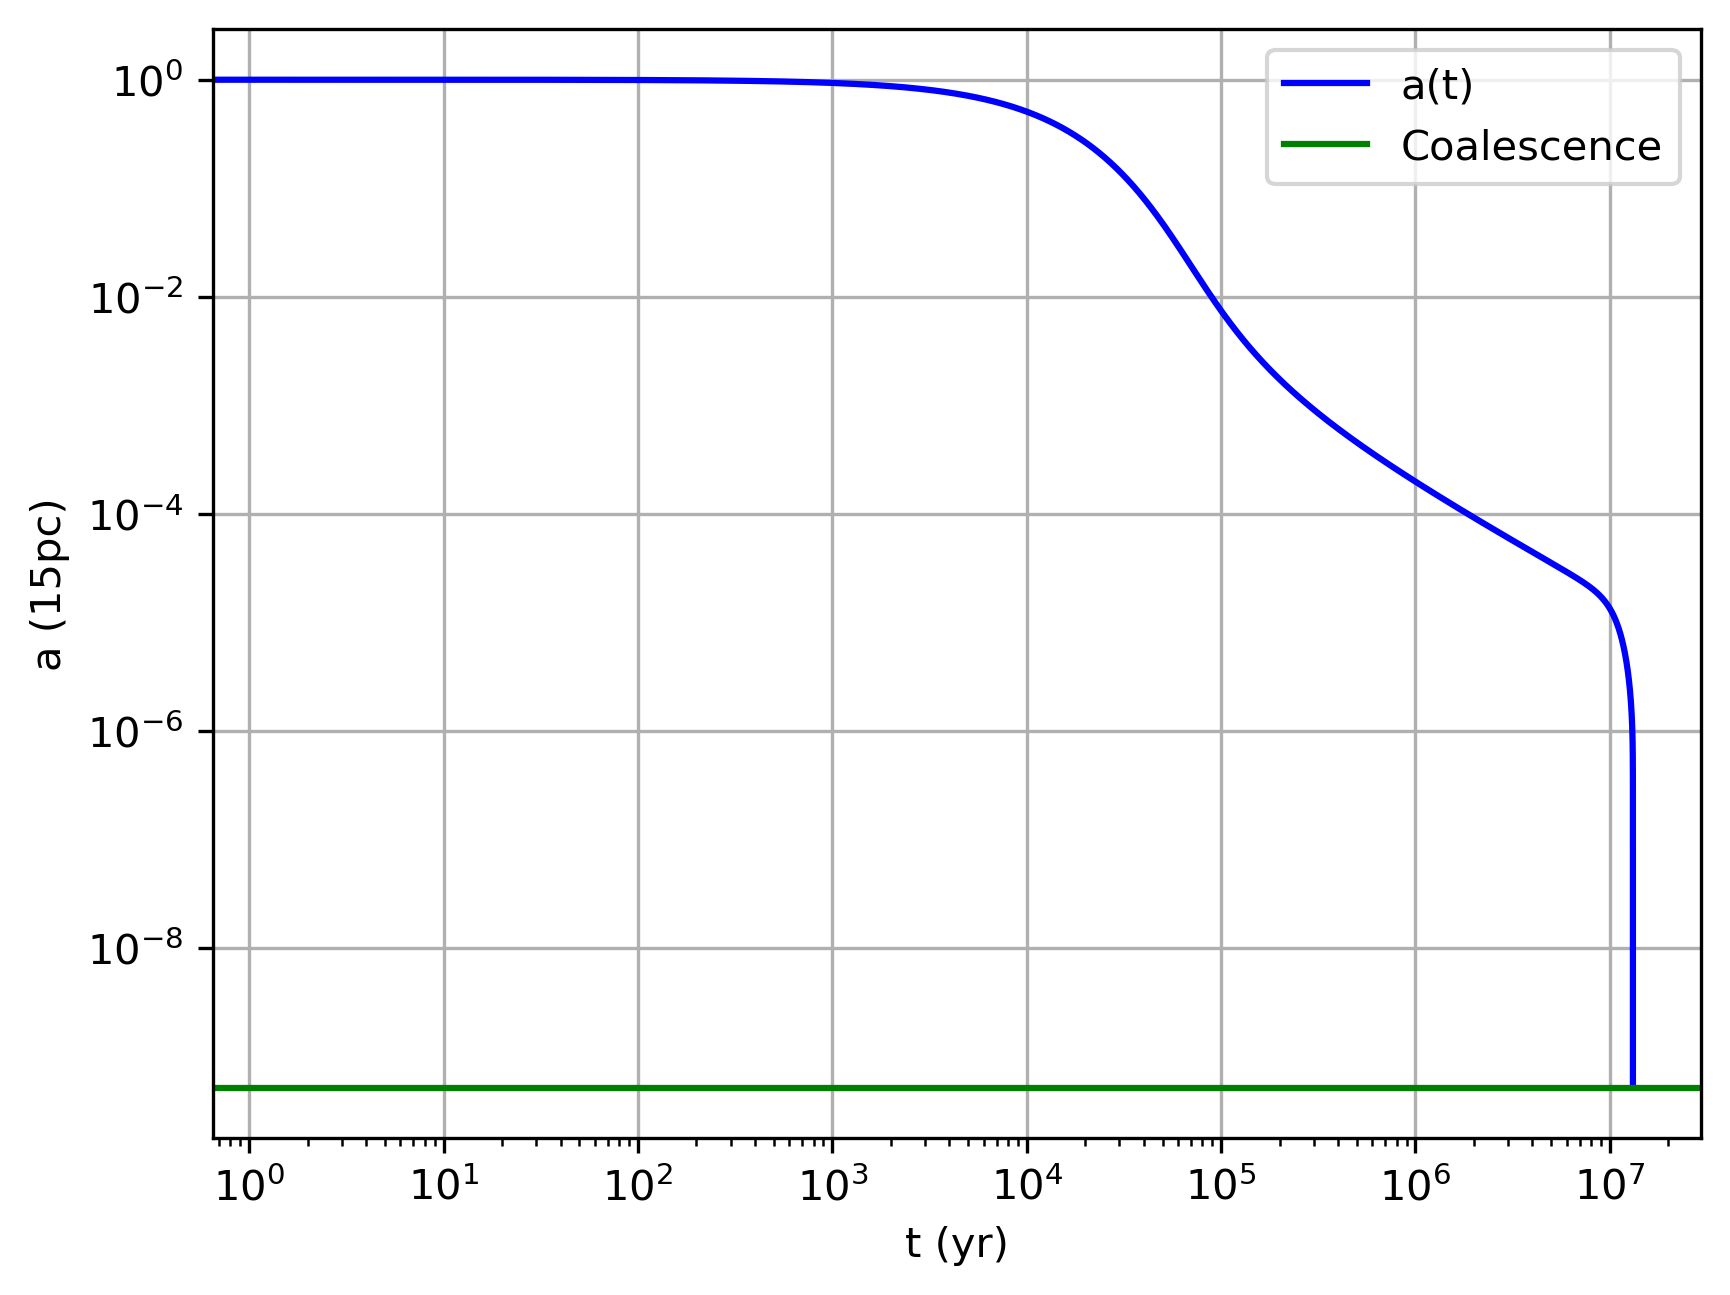
\includegraphics[width=0.5\linewidth]{NGC205_a_vs_t.png}
    \caption{NGC 205 a vs t}
    \label{NGC205 a vs t}
\end{figure}


\begin{figure}[H]
    \centering
    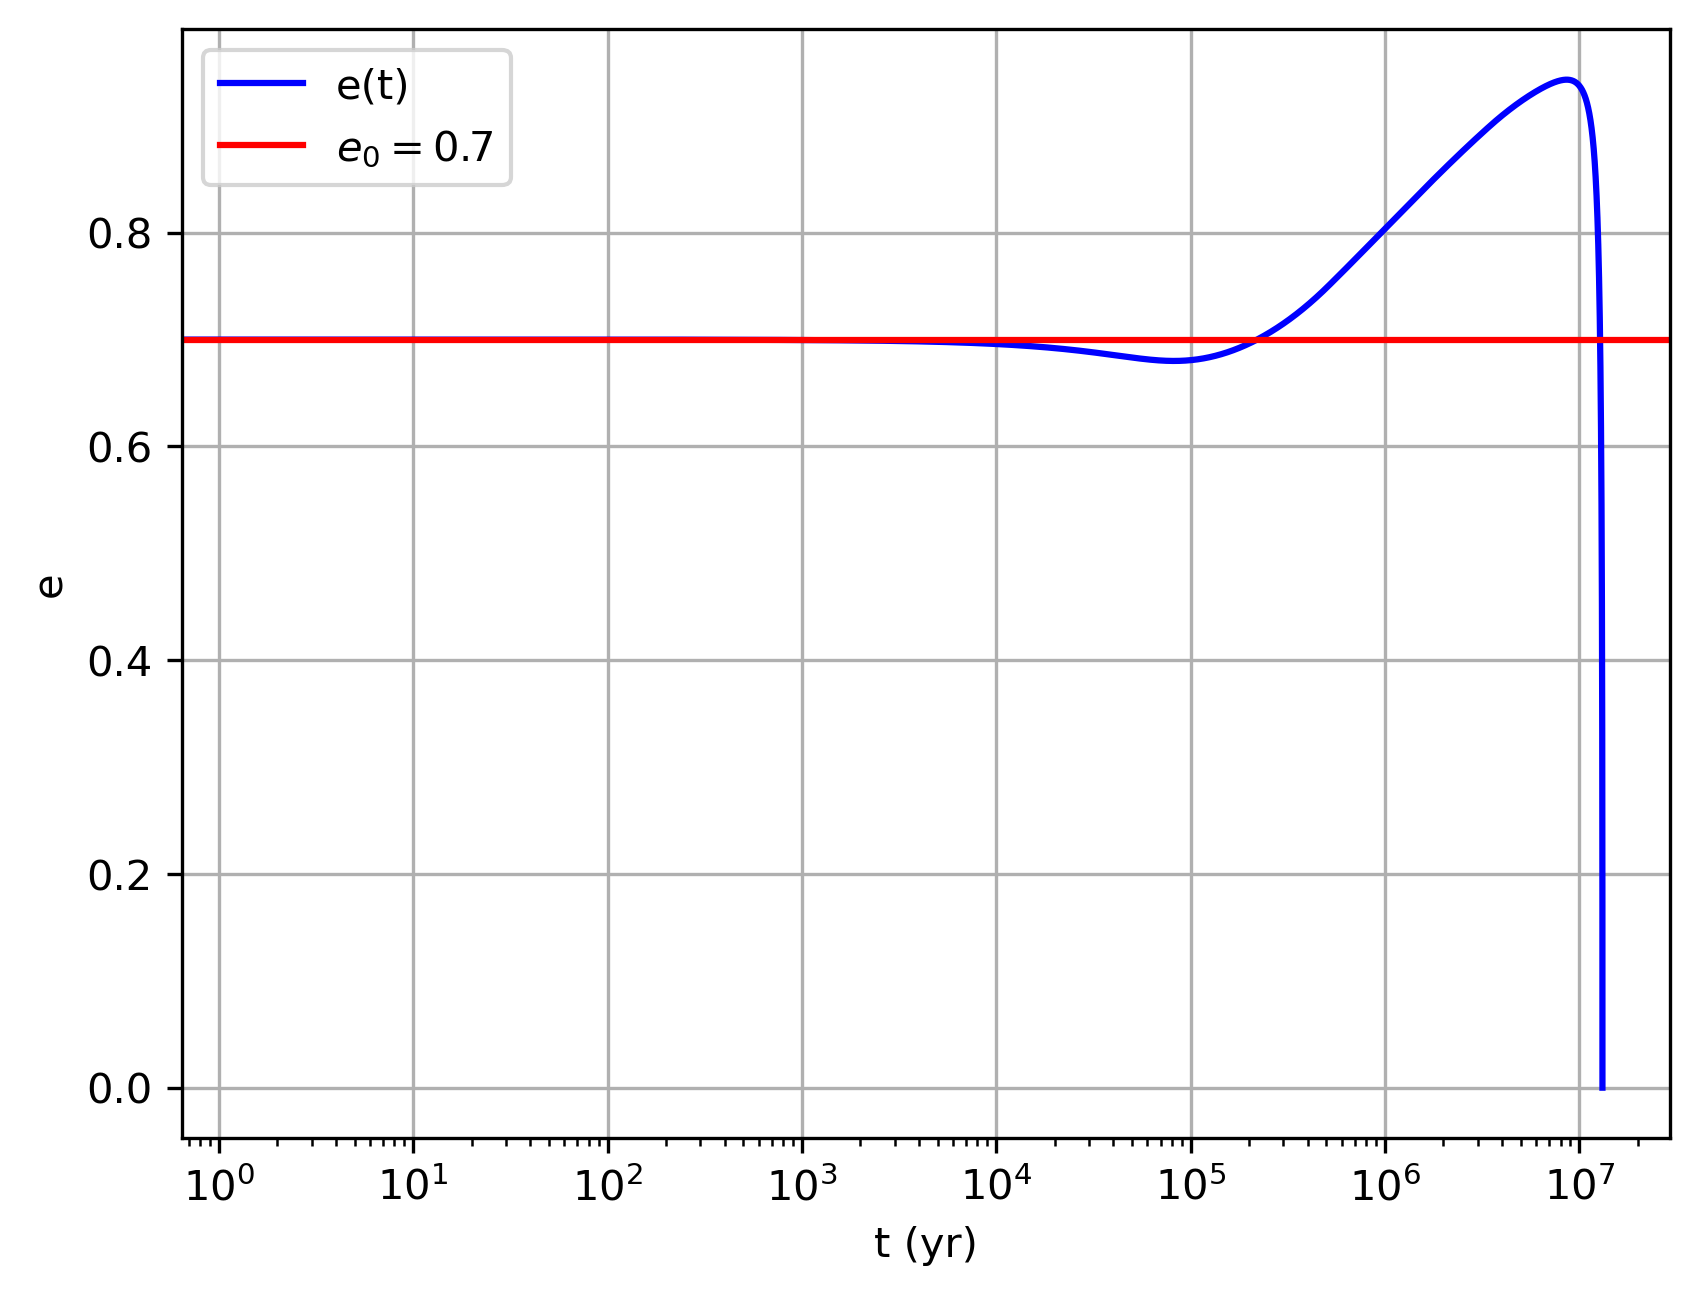
\includegraphics[width=0.5\linewidth]{NGC205_e_vs_t.png}
    \caption{NGC 205 e vs t}
    \label{NGC205 e vs t}
\end{figure}

The estimeted coalescence time is $t_{coal}=13.15 Myr$; it is of the same order of magnitude of\cite{Khan_2021} and \cite{Holley-Bockelmann_2025} predictions of $t_{coal}=74Myr$.\\$\mathbf{NOTE}$: Khan estimate comes from N-body simulations and in the special case of NGC 205 a costant value of eccentricity $e=0.39$ is assumed for the late evolution of the binary.\\Assuming a reliable time (universal time) at which the binary is in the configuration $(a_0,e_0)$ it might be interesting to get an estimate of the corresponding $z_{coal}$ from
\begin{equation}
t(z) = \int_z^{\infty}
\frac{dz'}{(1+z')H(z')}
\end{equation}
and compare it with LISA upper limit $(z\sim20)$, hence addressing the problem of a possible detection.\\If the binary is in the initial configuration at $z\approx 10$, it will coalesce at $z\approx 9.4$.

\subsection{Cosmic Size Evolution Down to NGC 205}
Here, we explore the importance of the existence of NSC to the binary evolution and coalescence time. A such structure is expected to drastically reduce the time taken by system to merge as a consequence of the larger number of stars capable of passing close to the binary.\\In this spirit, we will be referring to the same parameters table a procedure of the prevois SubSection but the NSC which is artificially removed from the dwarf galaxy; hence, the only stellar background affecting binary evolution is the stellar bulge.\\By repeating the same analysis and setting $(t_0,a_0,e_0)=(0yr,15pc,0.7)$, we show Figure \ref{NGC205 bulge a vs t plot} and \ref{NGC205 bulge e vs t plot}.

\begin{figure}[H]
    \centering
    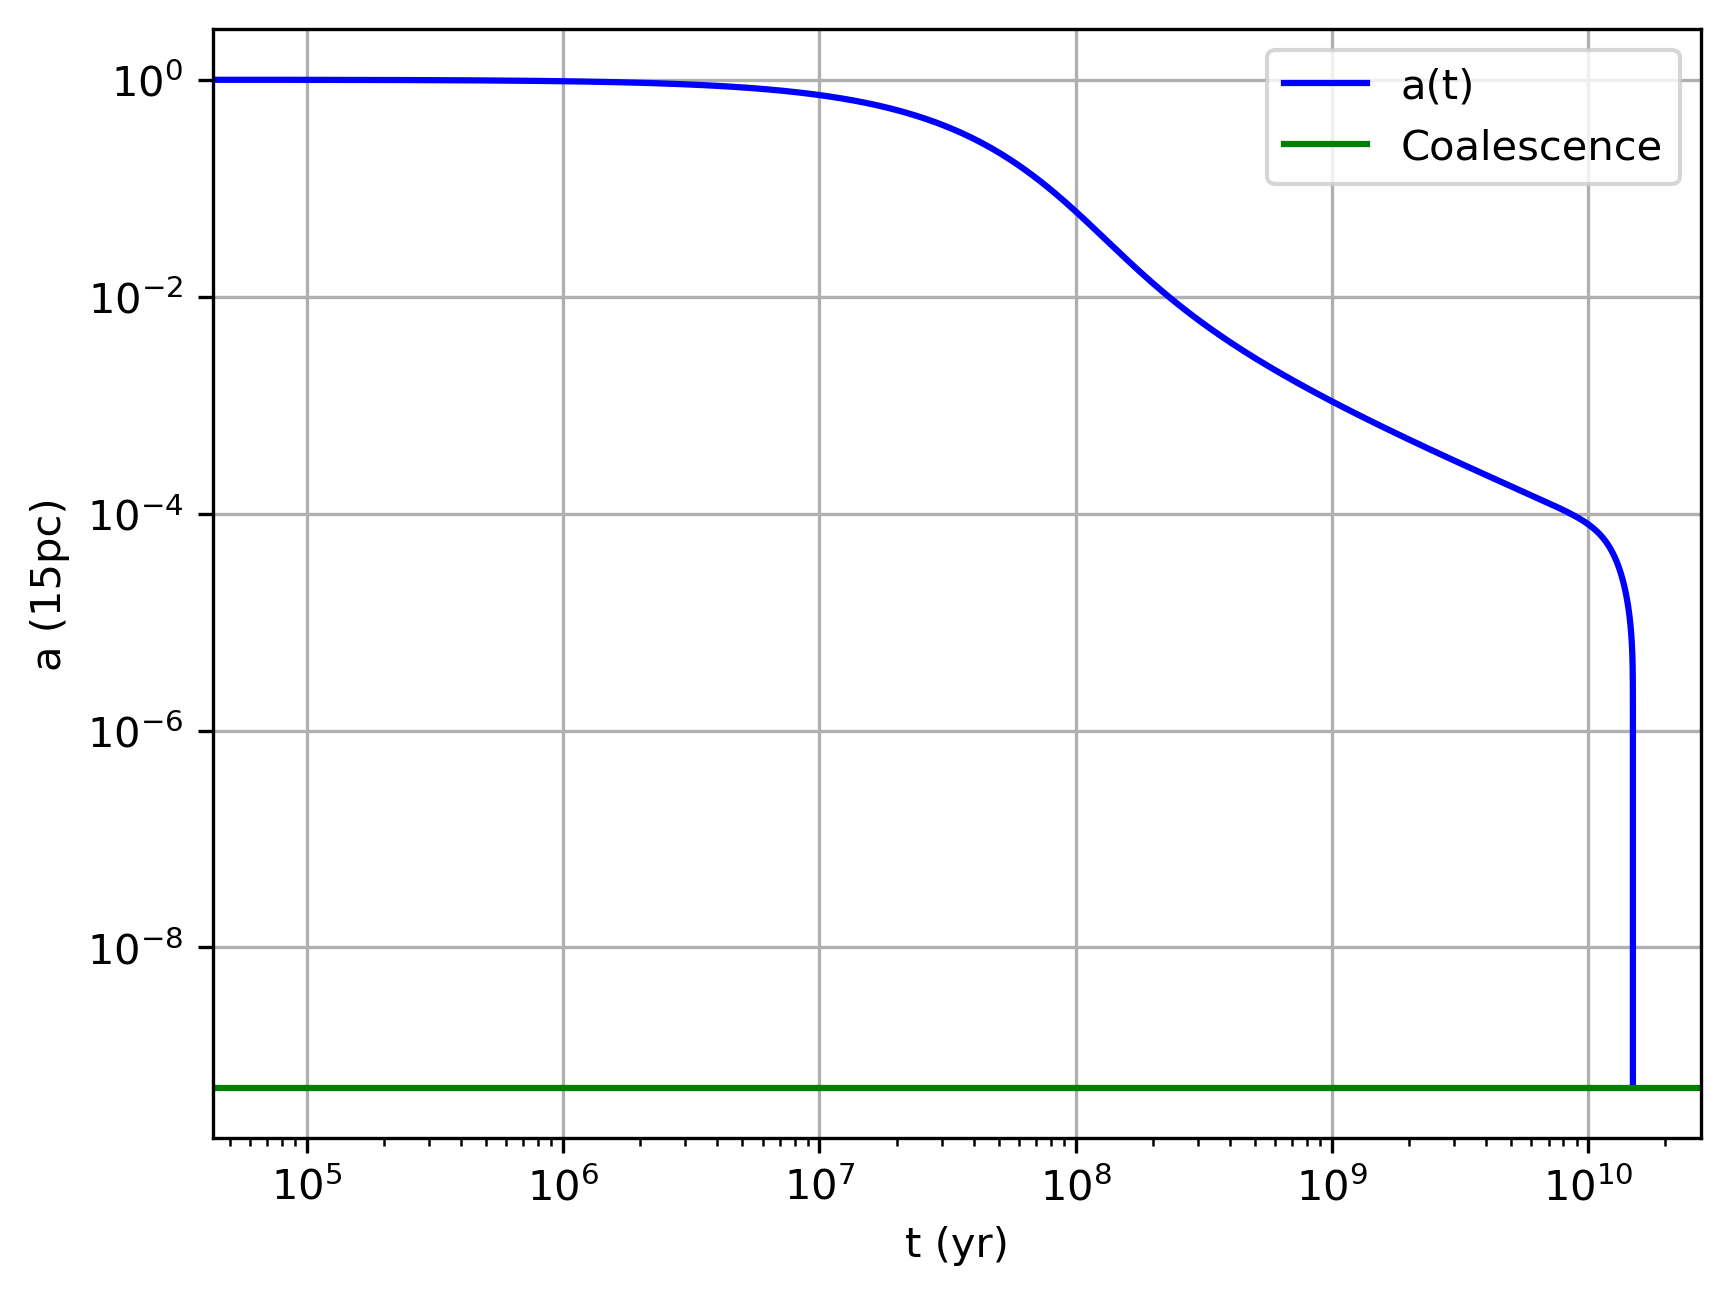
\includegraphics[width=0.5\linewidth]{NGC205_Bulge_a_vs_t.png}
    \caption{}
    \label{NGC205 bulge a vs t plot}
\end{figure}

\begin{figure}[H]
    \centering
    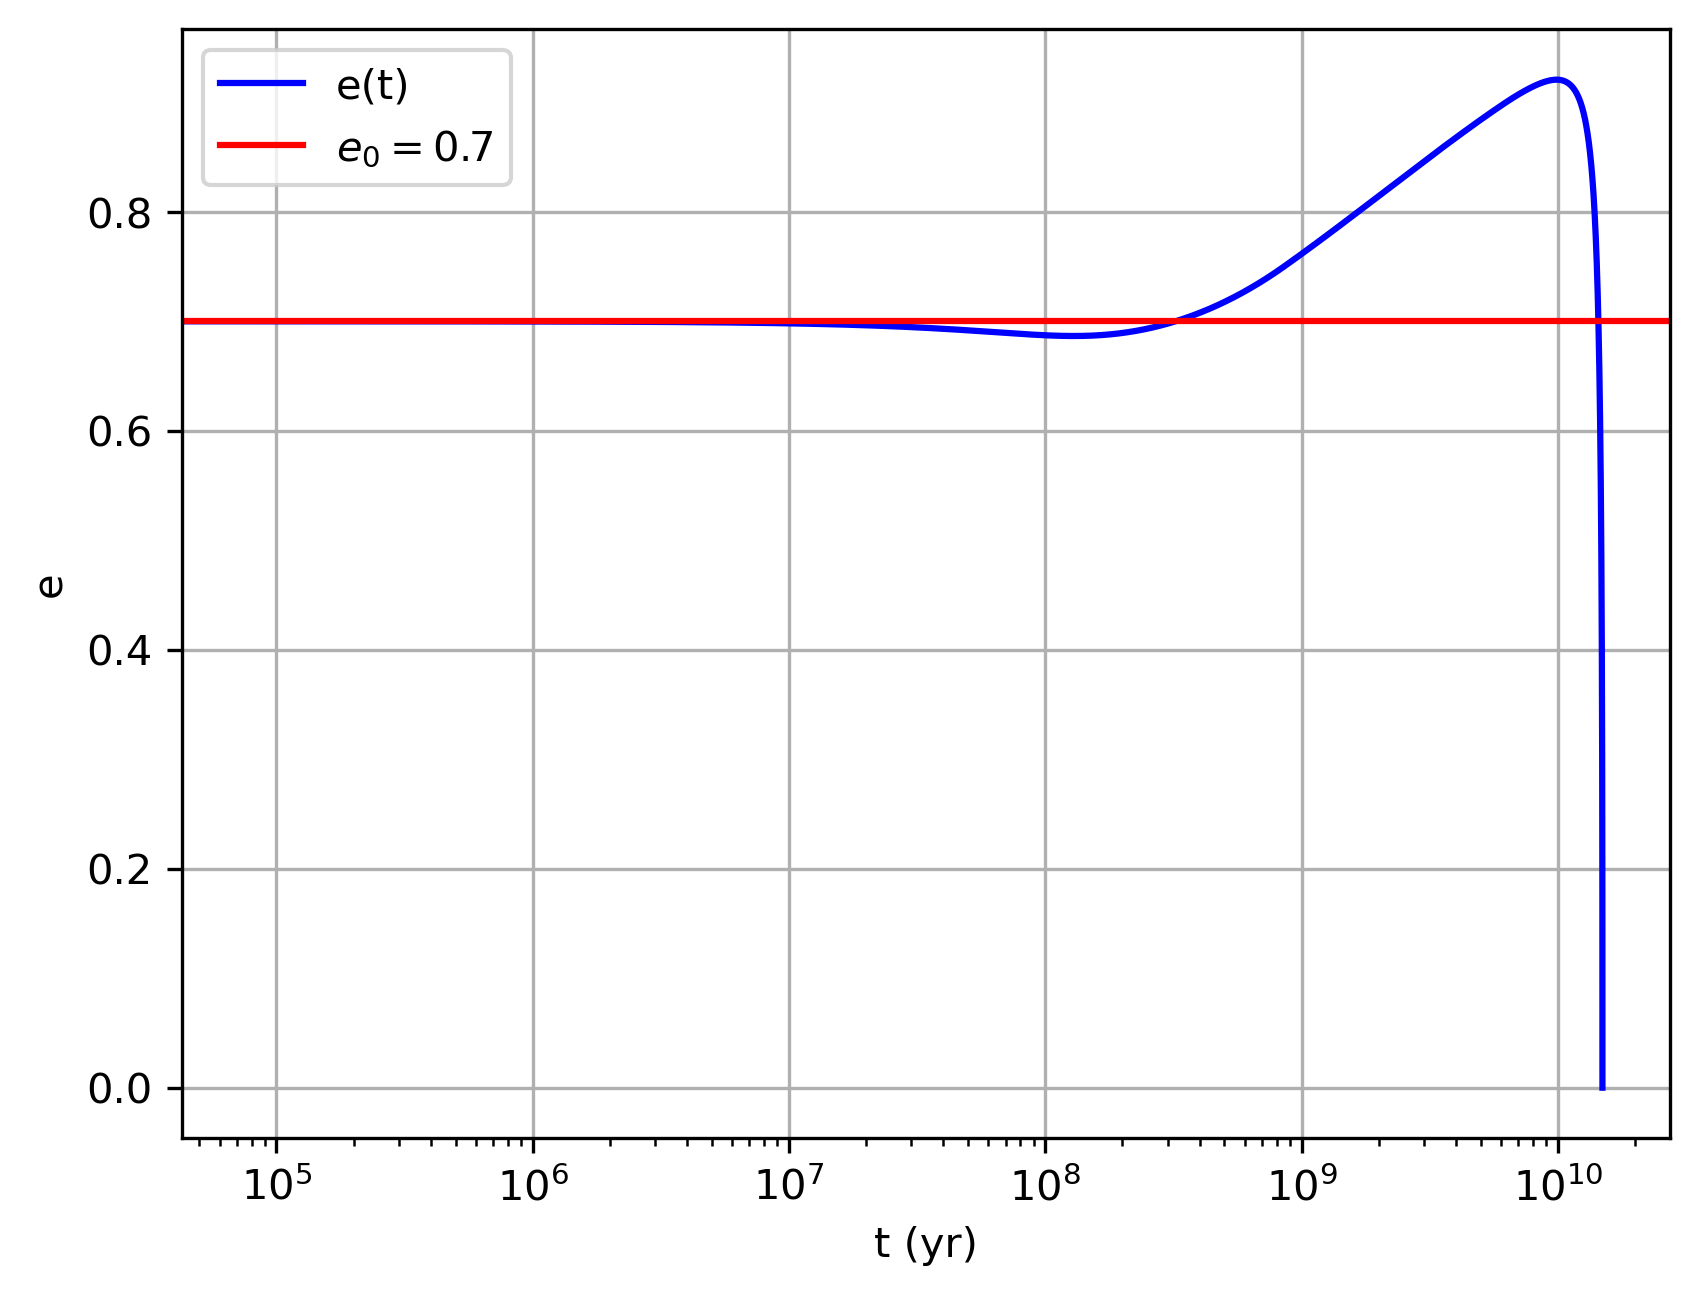
\includegraphics[width=0.5\linewidth]{NGC205_Bulge_e_vs_t.png}
    \caption{}
    \label{NGC205 bulge e vs t plot}
\end{figure}

Now $t_{coal}=14.93 Gyr$, almost three orders of magnitude longer than the NSC scenario.\\Following Ono cosmic size evolution relation $R_{eff}(z)=R_{eff}(z=0)(1+z)^{-1.22}$ \cite{Ono_2023}, we take NGC 205 as a $z=0$ reference model and we discuss the evolution of the same IMBH binary inside its plausible progenitors distributed between $z=1$ and $z=20$. All galaxies share same bulge mass and Sersic index; density profiles differ from each other only because of the different effective radius as diplayed in Figure \ref{Cosmic size density plot}.

\begin{figure}[H]
    \centering
    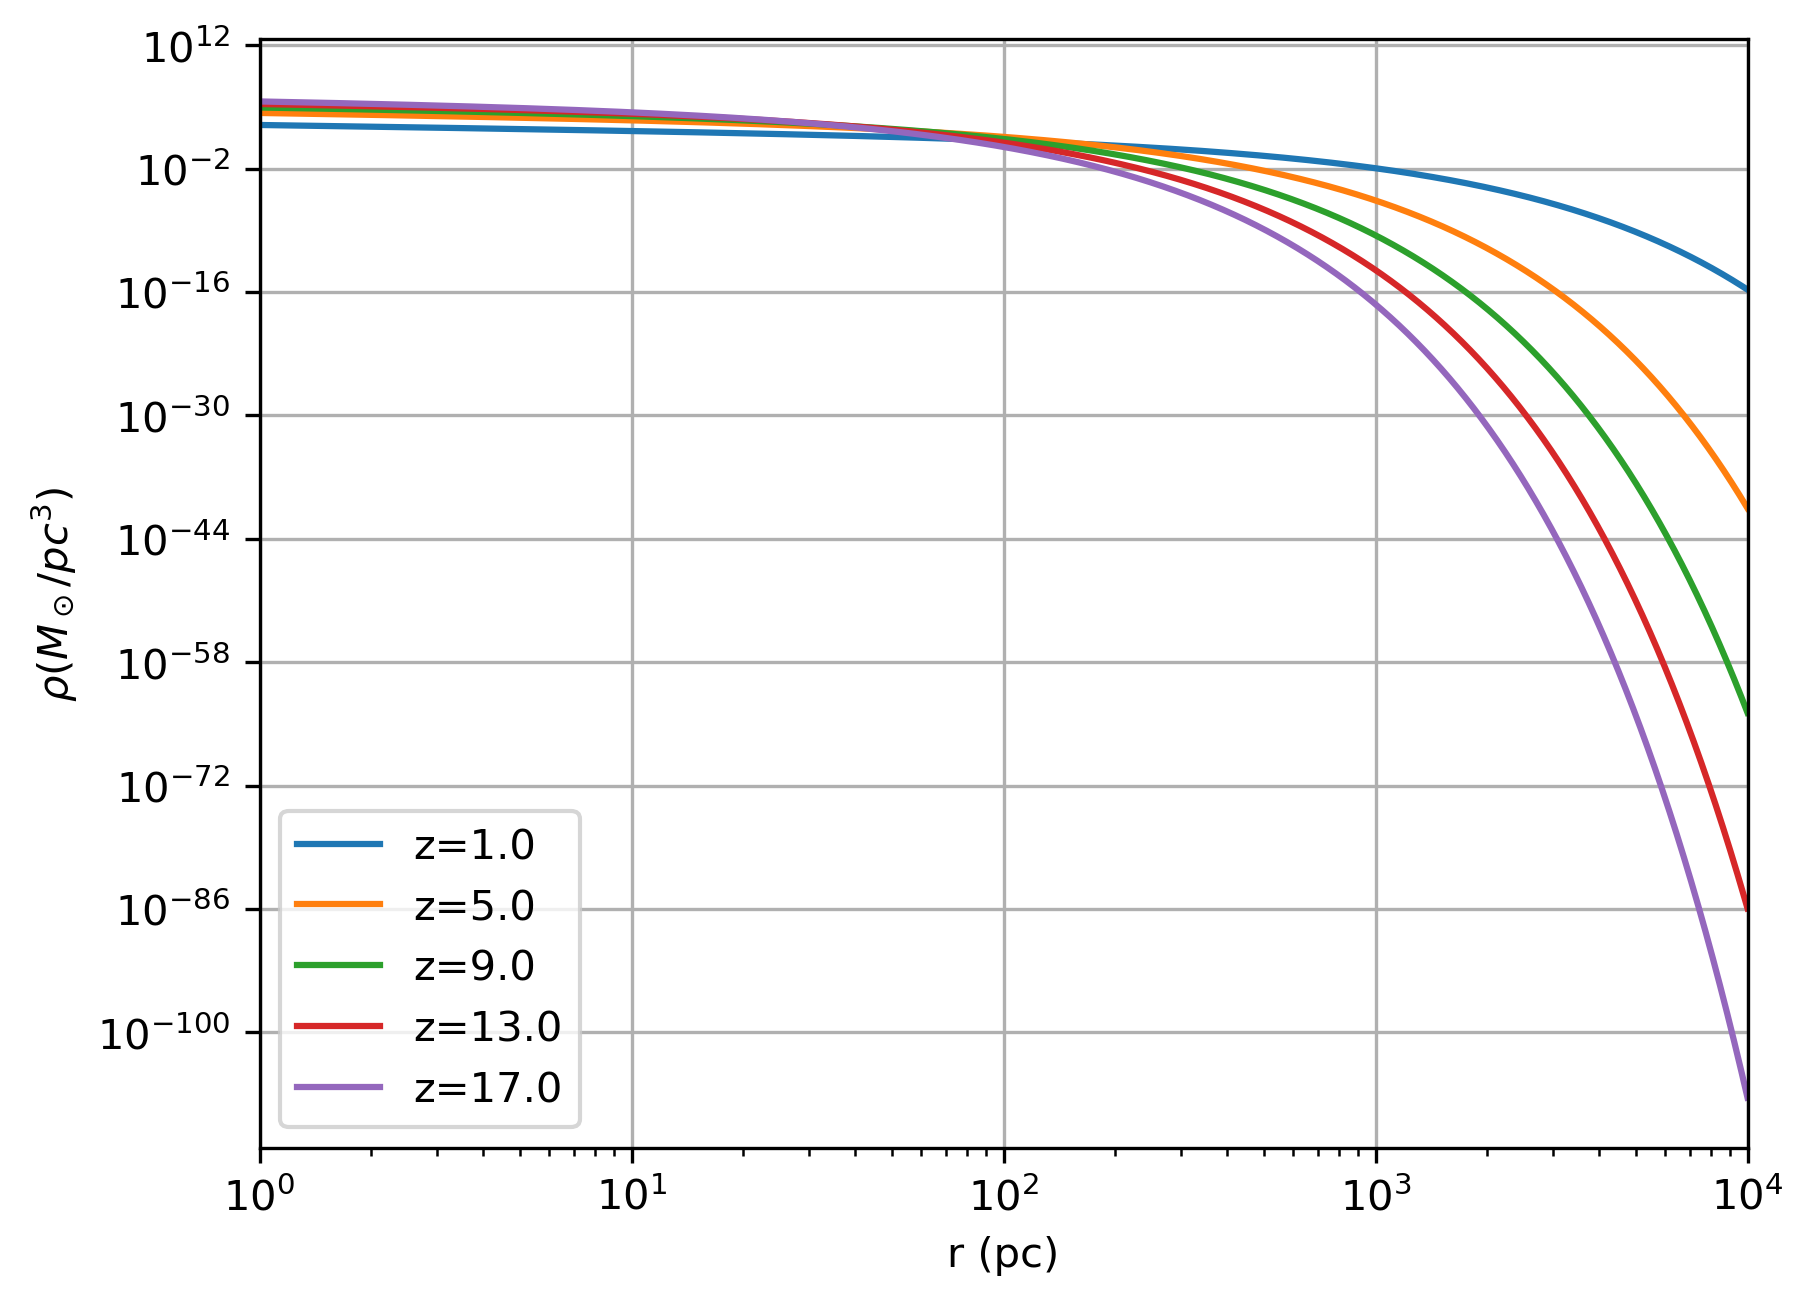
\includegraphics[width=0.5\linewidth]{Galaxies_density_profile.png}
    \caption{}
    \label{Cosmic size density plot}
\end{figure}
High redshift galaxies tend to be more compact than low redshift counterparts.\\Hardening radii are easly derived from these profiles according to Equation \ref{a_h dynamical definition} and a comparison between different hosts H and K functions- see Figure \ref{Cosmic size H plot} and \ref{Cosmic size K plot}- suggest that IMBH binary becomes "hard" at lower separation if embedded in a denser environment.
\begin{figure}[H]
    \centering
    
\includegraphics[width=0.5\linewidth]{Galaxies_H_unbound.png}
    \caption{}
    \label{Cosmic size H plot}
\end{figure}


\begin{figure}[H]
    \centering
    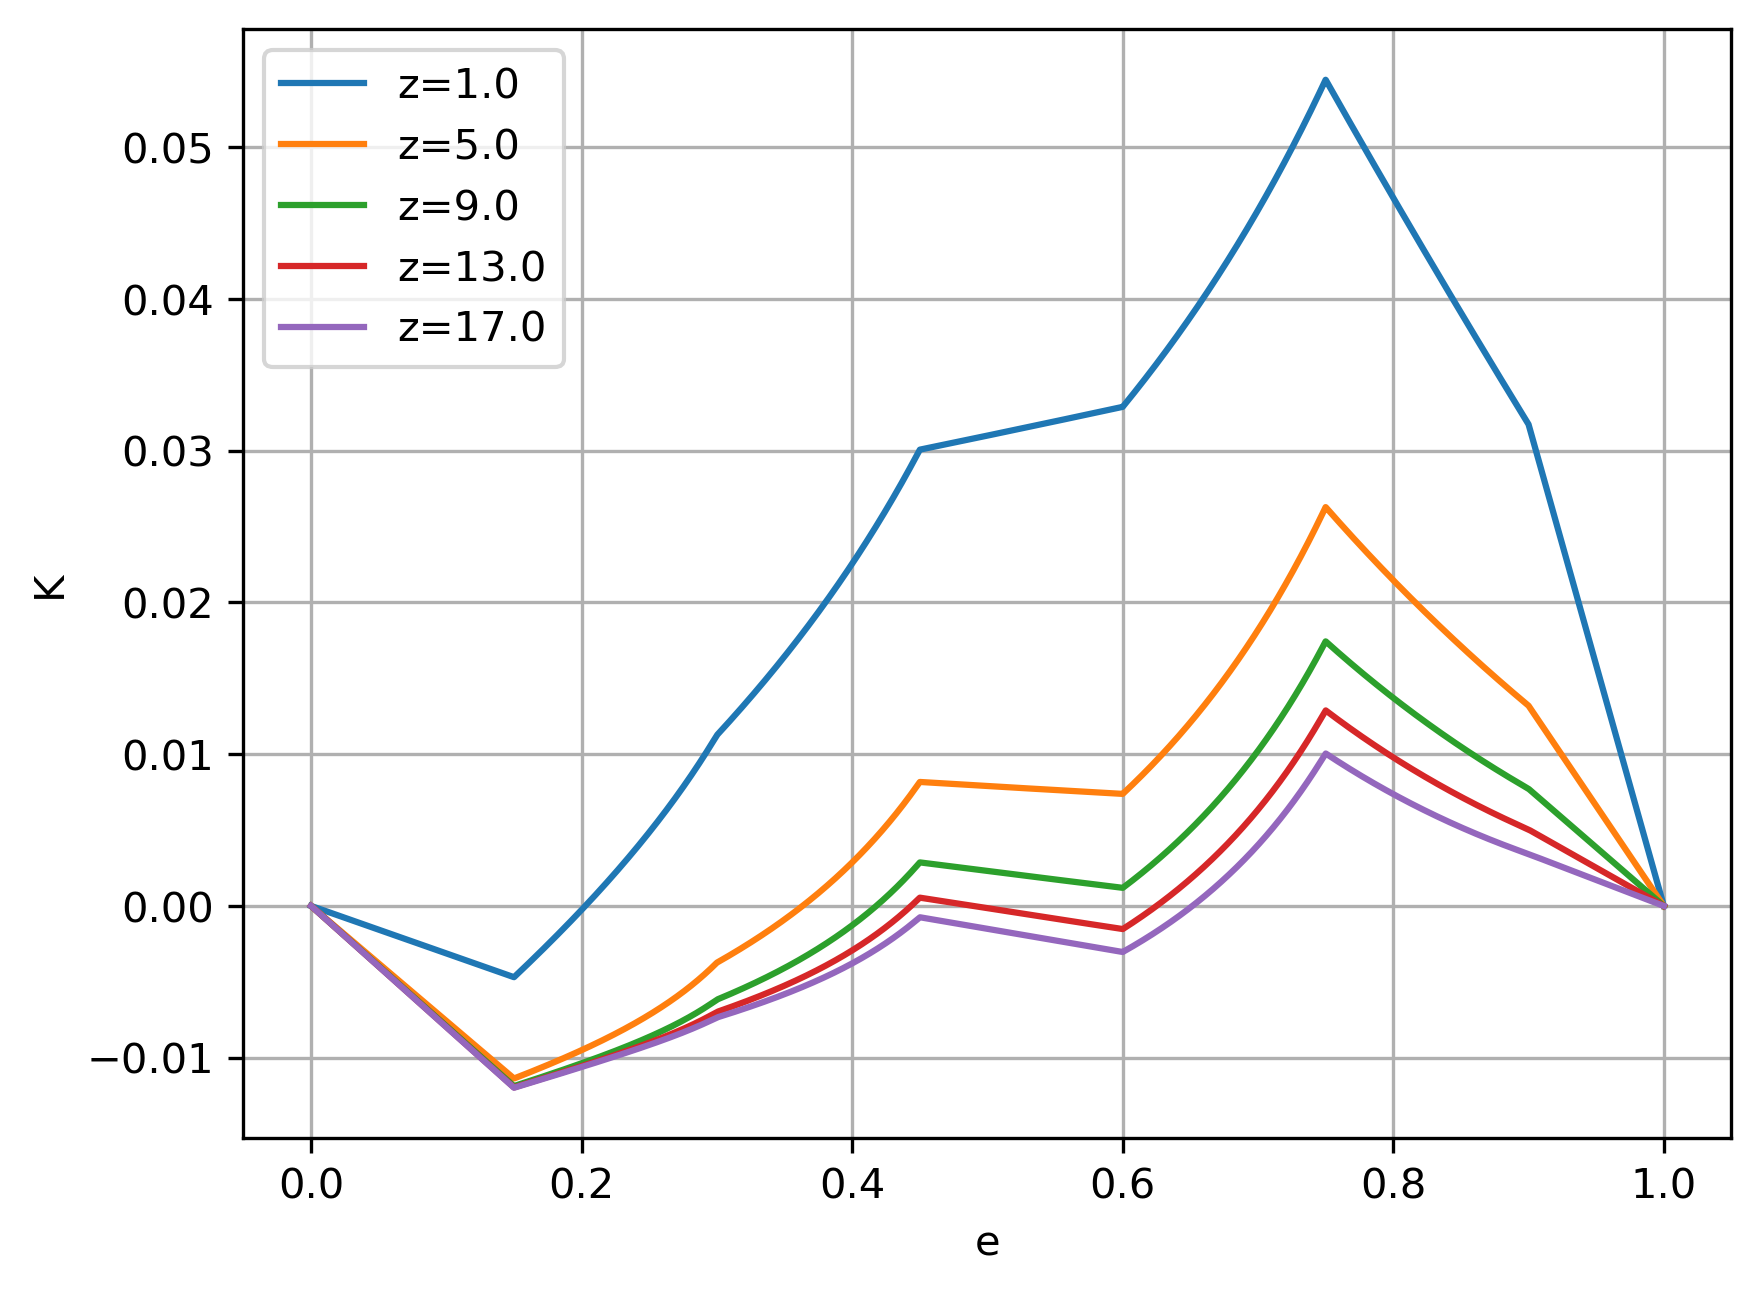
\includegraphics[width=0.5\linewidth]{Galaxies_K_unbound.png}
    \caption{This family of functions is obtained evaluating $K(a,e)$ of each galaxy at their mean hardening radius.}
    \label{Cosmic size K plot}
\end{figure}
We present in Figure \ref{Cosmic size a vs t plot} and \ref{Cosmic size e vs t plot} the evolutionary tracks of a sample of galaxies obtained by applying RK(4) to the Equations (\ref{da/dt Un+GW}) and (\ref{de/dt Un+GW}) and initial condition $(t_,a_0,e_0)=(0yr,15pc,0.7)$.
\begin{figure}[H]
    \centering
    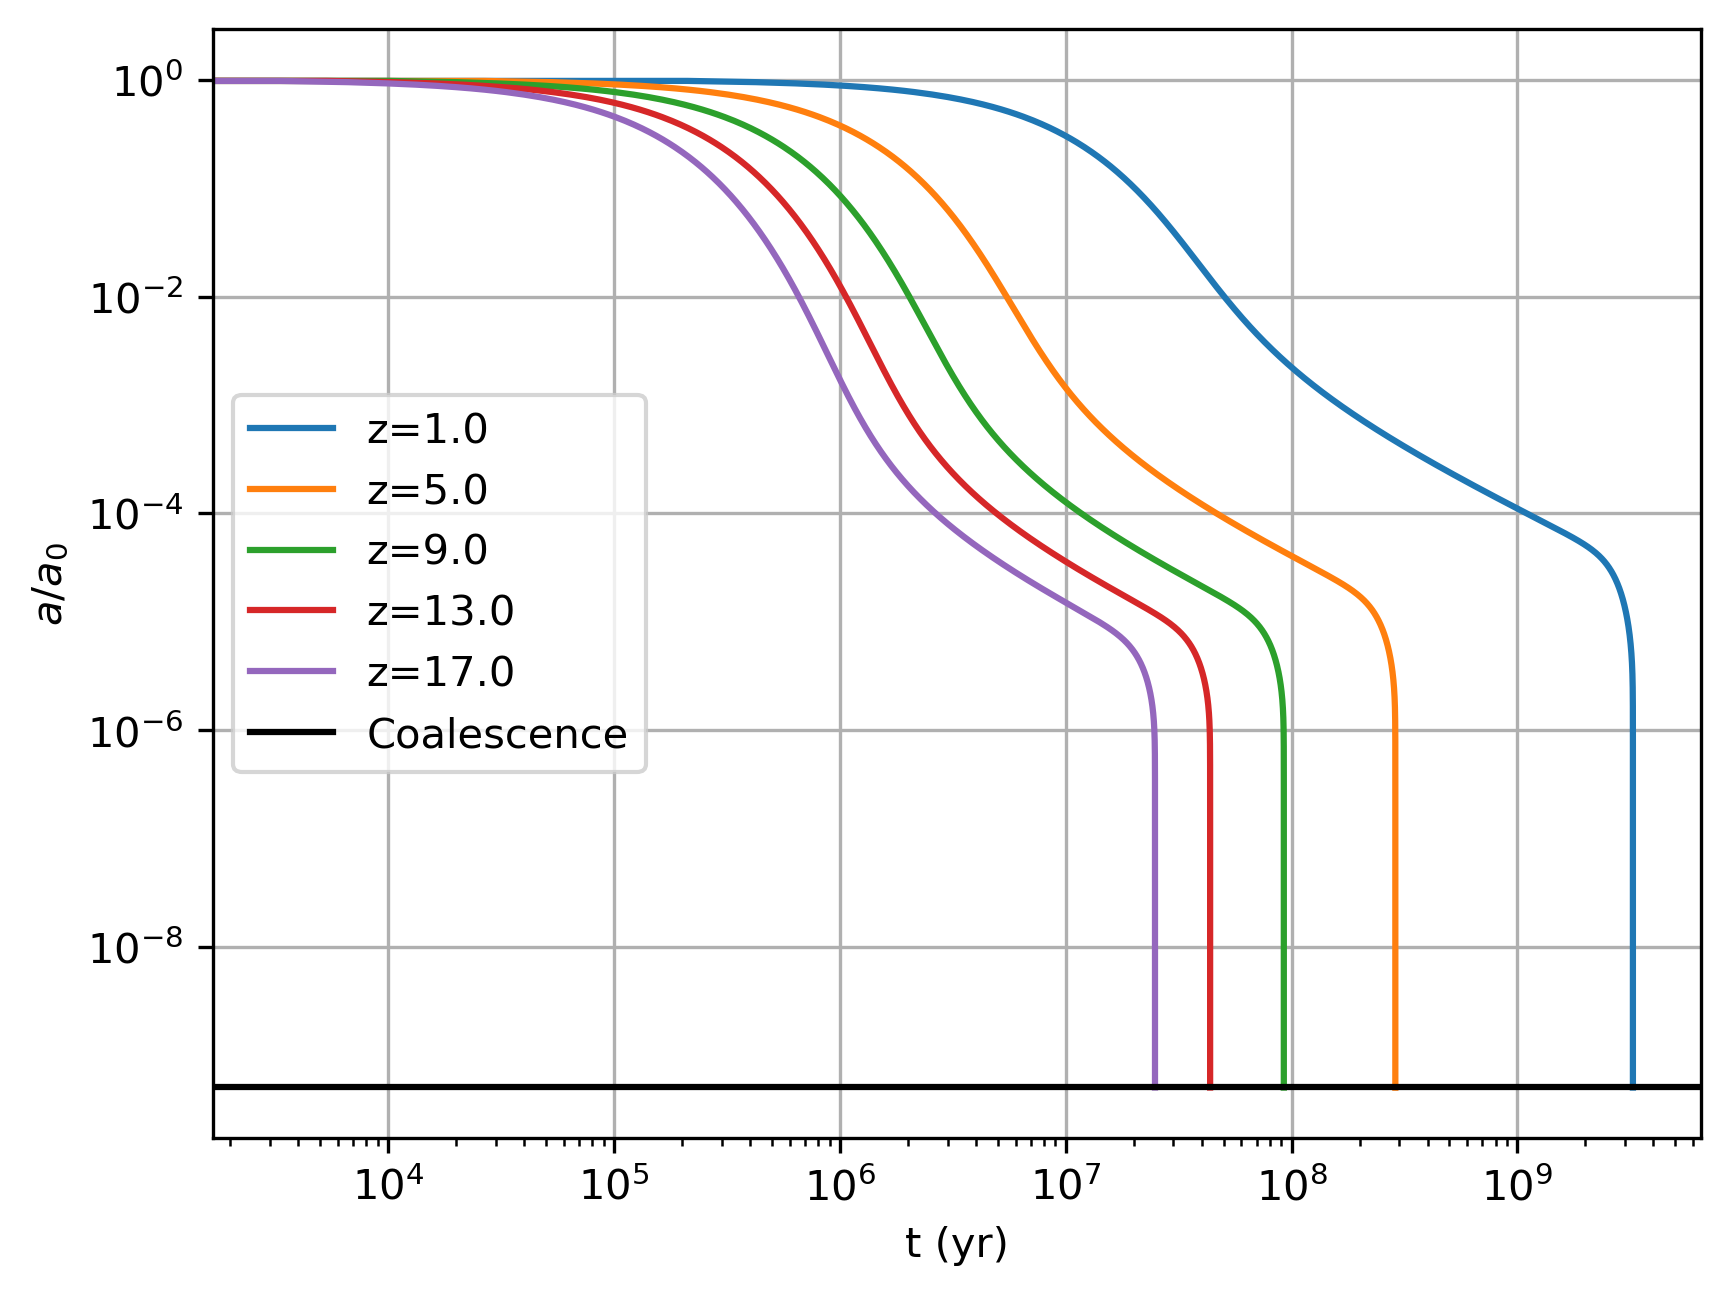
\includegraphics[width=0.5\linewidth]{Galaxies_a_vs_t.png}
    \caption{}
    \label{Cosmic size a vs t plot}
\end{figure}



\begin{figure}[H]
    \centering
    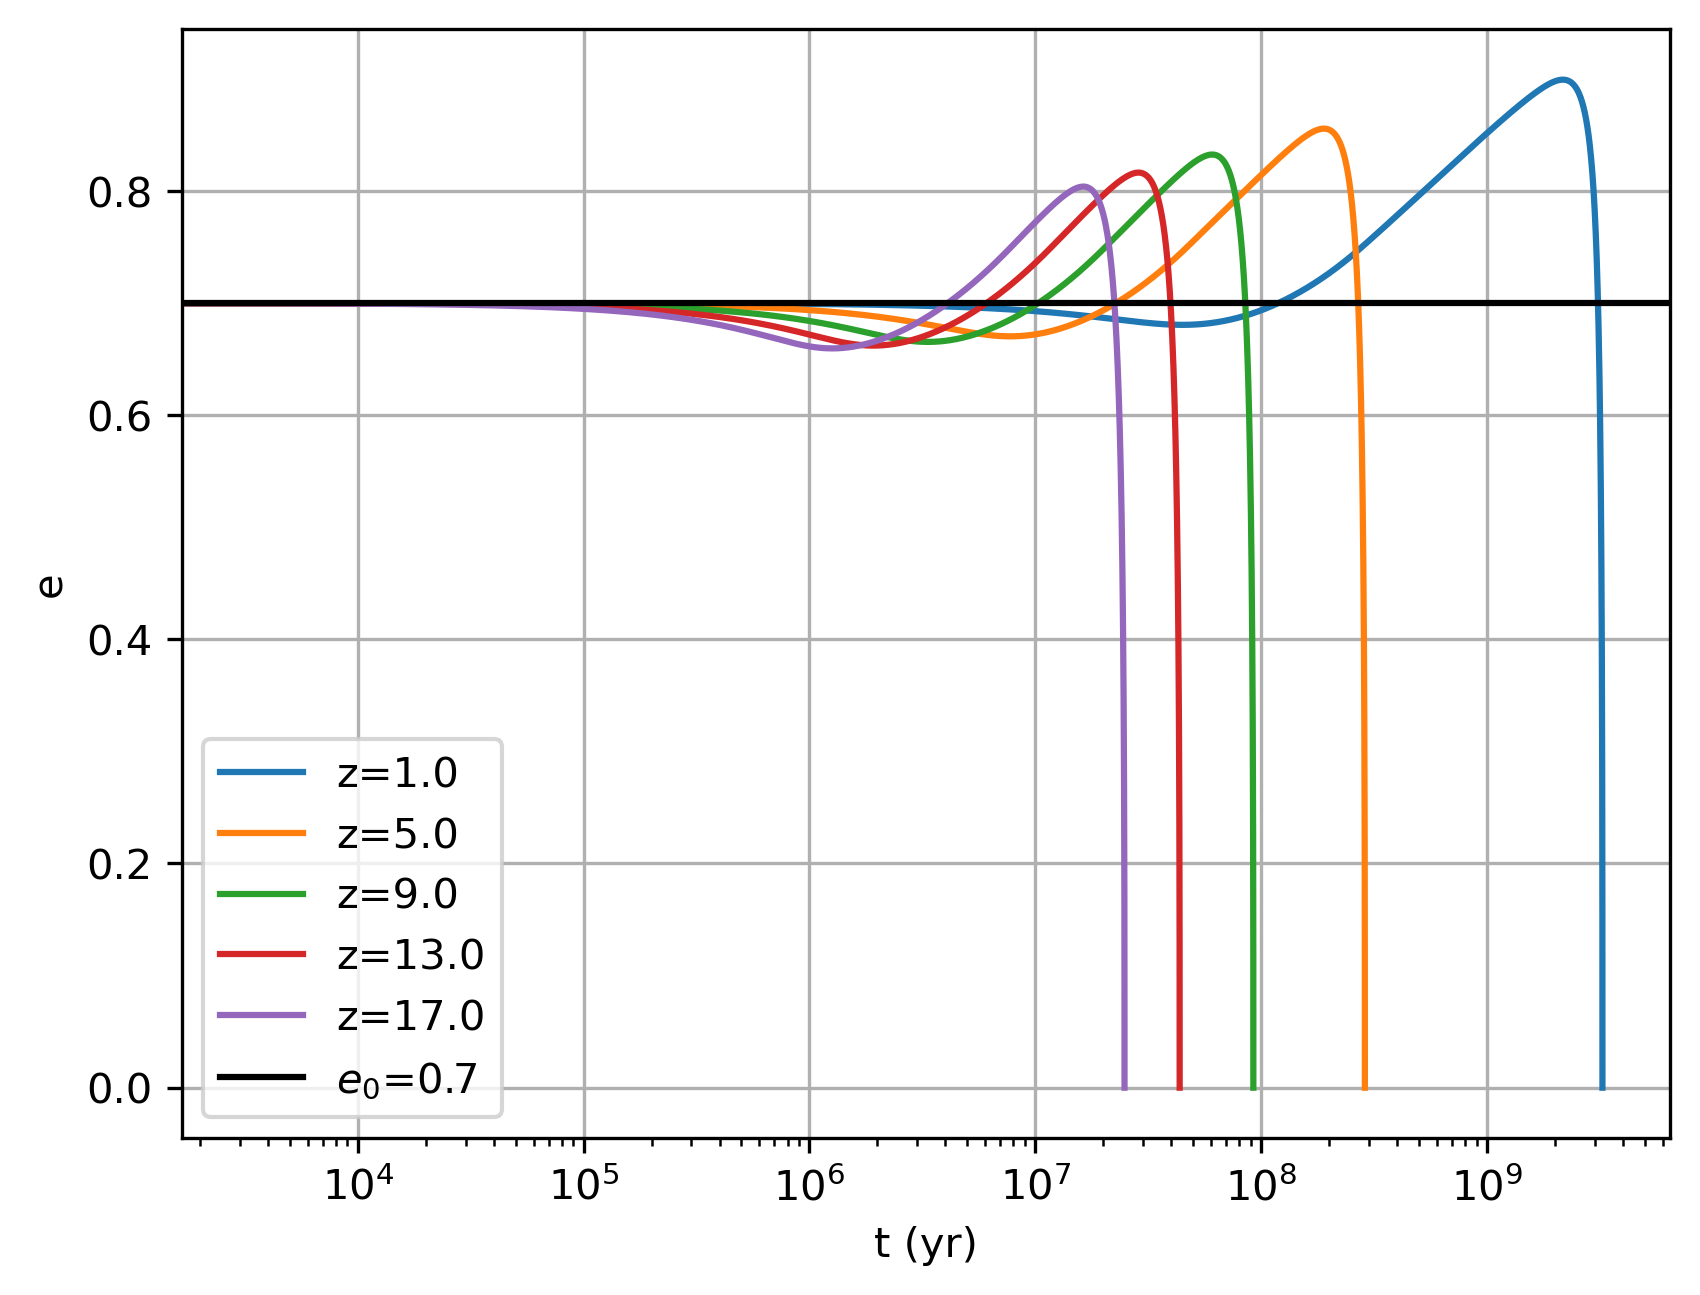
\includegraphics[width=0.5\linewidth]{Galaxies_e_vs_t.png}
    \caption{}
    \label{Cosmic size e vs t plot}
\end{figure}


\begin{table}[htbp]
\centering
\caption{Galaxies coalescence time grid (Gyr)}
\label{tab:example}
\begin{tabular}{ll}
\toprule
z & $t_{coal}$ (Gyr) \\
\midrule
 1  &  3.24728387   \\
 2  &  1.334011  \\
 3  &  0.7072763  \\
 4  &  0.43164087  \\
 5  &  0.28805534  \\
 6  &  0.20450559  \\
 7  &  0.15193439  \\
 8  &  0.11686942  \\
 9  &  0.09240003  \\
 10 &  0.07469761 \\
 11 &  0.06150781 \\
 12 &  0.05143637 \\
 13 &  0.04358488 \\
 14 &  0.03735426 \\
 15 &  0.03233322 \\
 16 &  0.02823207 \\
 17 &  0.02484224 \\
 18 &  0.02201059 \\
 19 &  0.01962278 \\
 20 &  0.01759202 \\
\bottomrule
\end{tabular}
\end{table}
We note that higher compactness tends to compensate the effects of NSC removal in terms of the coalescence time.\\Lastly, we modifiy the initial time $t_0$ of each run, turning it into $t(z)$, thus focusing on the possibility of coalescence within the present time and consequently a potential GWs observation.
\begin{figure}[H]
    \centering
    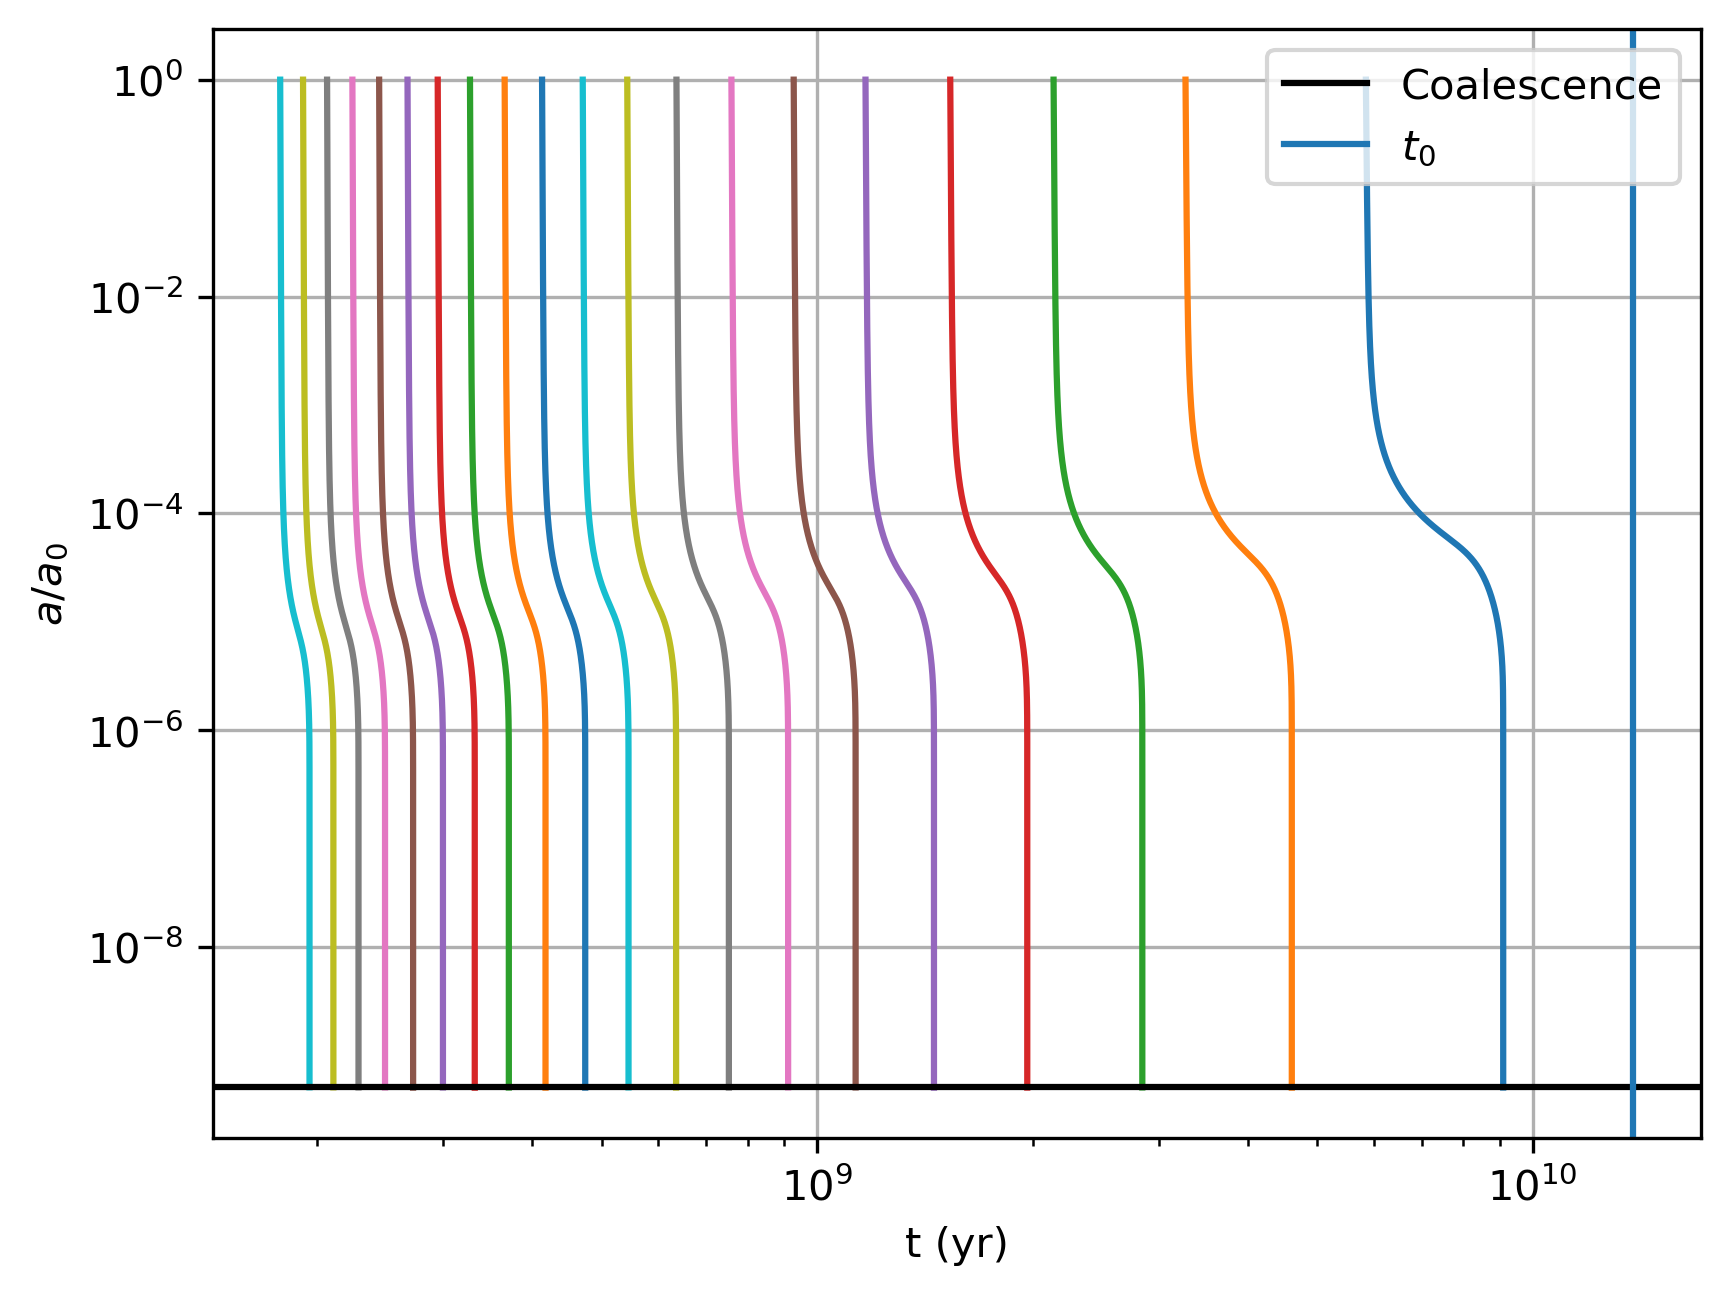
\includegraphics[width=0.5\linewidth]{Galaxies_a_vs_t_from_t(z).png}
    \caption{}
    \label{Cosmic size a vs t from t(z) plot}
\end{figure}
 
Therefore, forming in tha past at $z>0$, they all merge before the present time.







%\include{Chapter_4}






\chapter{Generation of Initial Conditions for N-body Stellar Systems}\label{chap:chapter3}


\section{Dynamical Equilibrium of Stellar Systems}
Galaxies are multi-component systems in dynamical equilibrium, where different stellar populations, gaseous phases, dust, and dark matter coexist. These environments host an enormous number of stars, typically ranging from ,which makes it impossible to track the orbit of each individual object. Neverthless, by abandoning the idea of characterizing the time evolution of each degree of freedom in the phase-space, a probabilistic description of the stellar population is still possible in terms of the one-particle DF as anticipated in Section 1.1.\\As long as the stellar component is observed within $t_{2b}$, granularity  is unimportant, collisions are negligible and stars can be described as particles moving in a smooth potential
generated by a continous mass density $\rho$, proxy of the actual stellar distribution. In this regime, when dealing with stars that are all identical to one another, the DF will be unique and will satisfy the Collisionless Boltzmann Equation (CBE). By denoting with $\mathbf{w}$ an arbitrary set of canonical coordinates of PS, this conservation equation descends from differentiating with respect to the time---along the orbits of the potential $\Phi(\mathbf{x},t)$ associated to $\rho(\mathbf{x},t)$---of the normalization condition

\begin{equation}\label{DF normalization}
 \int_{\mathbb{R}^6}d\mathbf{w}\, f(\mathbf{w})=1.
\end{equation}
By extending the Lagrangian derivative notion $D/Dt$ to the coordinates of the phase-space, the CBE reads:

\begin{equation}\label{CBE}
    \frac{Df}{Dt}=\frac{\partial f}{\partial t}+
    \mathbf{\dot{w}}\cdot \frac{\partial f}{\partial \mathbf{w}}=
    \frac{\partial f}{\partial t}+[f,H]=0,
\end{equation}
where the square bracket indicates the Poisson bracket, which is defined as

\begin{equation}\label{Poisson bracket}
[f,H]
=
\sum_i
\left(
\frac{\partial f}{\partial q_i}
\frac{\partial H}{\partial p_i}
-
\frac{\partial f}{\partial p_i}
\frac{\partial H}{\partial q_i}
\right),
\end{equation}
and $H$ is the Hamiltonian function of the system.\\The arbitrariness of the canonical coordinates $\mathbf{w}$ enables us to specialize Equation (\ref{CBE}) to the inertial Cartesian coordinates $(\mathbf{x},\mathbf{v})$. With this choice, the Hamiltonian becomes
\begin{equation}\label{Hamiltonian in cartesian coord.}
    H(\mathbf{x},\mathbf{v},t)=\frac{1}{2}v^2+\Phi(\mathbf{x},t)
\end{equation}
and the CBE turns into
\begin{equation}\label{CBE in cartesian coord.}
    \frac{\partial f}{\partial t}+\mathbf{v}\cdot
    \frac{\partial f}{\partial \mathbf{x}}-
    \frac{\partial \Phi}{\partial \mathbf{x}}
    \cdot \frac{\partial f}{\partial \mathbf{v}}=0.
\end{equation}
Being interested in studying the equilibrium condition of galaxies and in particular of spherically symmetric models, it is usefull the following definition: a dynamical system is said to be stationary if $\partial f/\partial t=0$. Therefore, collisionless systems that have achieved equilibrium will be provided of a DF obeying to the steady-state CBE
\begin{equation}\label{Stationary CBE}
    \frac{Df}{Dt}=
    \mathbf{\dot{w}}\cdot \frac{\partial f}{\partial \mathbf{w}}=
    [f,H]=0.
\end{equation}
Noteworthy, for this condition to apply it is sufficient to have a steady-state potential $\Phi(\mathbf{x},\mathbf{v})$.
Solutions to Equation (\ref{Stationary CBE}) are referred to as integrals of motion. Specifically, the function $I(\mathbf{x},\mathbf{v})$ is an integral of motion for the potential $\Phi(\mathbf{x},\mathbf{v})$ if it satisfies
\begin{equation}\label{Integral of motion def}
    \frac{D}{Dt}[I(\mathbf{x}(t),\mathbf{v}(t))]=0
\end{equation}
along any orbit of the potential and a relevant example is represented by the Hamiltonian itself of the system, provided
\begin{equation}
 [H,H]=0.
\end{equation}
The comparison between Equation (\ref{Integral of motion def}) and Equation (\ref{Stationary CBE}) reveals that solving the steady-state CBE is equivalent to being an integral of motion; this leads to the formulation of the Jeans theorem.
\medskip

\noindent\textbf{Jeans Theorem. --}
\emph{Any steady-state solution of the collisionless Boltzmann equation depends on
the phase-space coordinates only through integrals of motion in the given potential, and any function of the integrals yields a steady-state solution of the collisionless Boltzmann
equation.}
\medskip

\noindent The remaining quantities to be defined, which correspond to observables that can be inferred from kinematic measurements, are the first- and second-order velocity moments of the distribution function. These are

\begin{equation}\label{mean velocity of DF}
    \overline{v_i}(\mathbf{x},t)\equiv 
    \frac{1}{\rho(\mathbf{x},t)}\int_{\mathbb{R}^6} d^3 \mathbf{v}\,f v_i
\end{equation}
and
\begin{equation}\label{velocity-dispersion of DF}
    \sigma_{ij}^2(\mathbf{x},t)\equiv 
    \frac{1}{\rho(\mathbf{x},t)}\int_{\mathbb{R}^6} d^3 \mathbf{v}\,
    f (v_i-\overline{v_i})(v_j-\overline{v_j})=\overline{v_iv_j}-
    \overline{v_i}\,\overline{v_j},
\end{equation}
respectively the mean velocity and the velocity dispersion tensor.\\We are now finally in a position to recall the most peculiar kinematical properties of an important subclass of equilibrium models, namely Ergodic systems. The Jeans Theorem imposes that the DF $f$ of systems at equilibrium will be any non-negative function of $H$; in case $f$ depends on $H$ only, i.e. $f=f(H)$, then systems with this type of DF are said Ergodic.\\Let us focus on first-order moment of the DF. In the inertial Cartesian frame where stars move under the action of a steady-state potential $\Phi(\mathbf{x})$, the Hamiltonian of the system is an even function of $\mathbf{v}$, causing $\overline{v_x}(\mathbf{x})=\overline{v_y}(\mathbf{x})=\overline{v_z}(\mathbf{x})$ to vanish.\\Similarly, it can be demonstrated that the velocity-dispersion tensor is isotropic; thus it holds
\begin{equation}\label{Ergodic velocity dispersion tensor}
 \sigma^2_{ij}(\mathbf{x})=\sigma^2(\mathbf{x})\delta_{ij}=\delta_{ij}\frac{4\pi}{3\rho(\mathbf{x})}\int_0^{+\infty}dv\,v^4f\left(\frac{1}{2}v^2+\Phi(\mathbf{x})\right)
\end{equation}
Therefore, every system characterized by an ergodic DF is isotropic. In the next Section, the properties of the generated steady-state isotropic stellar distributions will be presented and compared with the theoretical predictions summarized above.\\So far, we have been concerned with the velocity-moments of the distribution function of Ergodic systems; however, the generation of initial conditions (ICs) for N-body, equilibrium models relies on the correct sampling of the DF itself. Recovering it from $\rho$ for globally isotropic stellar systems can be done by means of the Eddington's formula
\begin{equation}\label{Eddington's formula}
f(\varepsilon)=\frac{1}{\sqrt{8}\pi^2}\frac{d}{d\varepsilon}
\int_{\varepsilon_t}^{\varepsilon}
\frac{d\rho}{d\Psi}\frac{d\Psi}{\sqrt{\varepsilon-\Psi}}
\end{equation}
with $\varepsilon=-H$ and $\Psi=-\Phi$ being the relative energy and potential respectively
and $\varepsilon_t$ the truncation energy of the system.\\Finally, the last tool introduced in this Section is the virial ratio, closely connected with the Virial theorem, which provides a fast diagnostic for determining whether the generated model is in equilibrium or is either evolving toward collapse or expansion. By definition a self-gravitating system, constituted by N particles, with total kinteic energy
\begin{equation}
K = \sum_{i=1}^{N} \frac{1}{2} m_i v_i^2
\end{equation}
and gravitational potential energy
\begin{equation}
U = -\frac{1}{2} \sum_{i=1}^{N} \sum_{j \ne i} \frac{Gm_i m_j}{|\mathbf{x_i}-\mathbf{x_j}|}
\end{equation}
is virialized if it holds
\begin{equation}
   2K'+U=0 \qquad \forall t
\end{equation}
in the barycentric inertial reference system $S_{CM}$. For these systems the virial ratio
\begin{equation}\label{virial ratio}
    Q\equiv\frac{2K'}{|U|}
\end{equation}
should be close to unity. In presence of a non vanishing velocity of the system center of mass, which flags that the time evolution is studied in a frame $S$ moving with respet to $S_{CM}$, Equation (\ref{virial ratio}) must be adjusted as follows:
\begin{equation}\label{virial ratio without offset}
    Q\equiv\frac{2(K-K_{CM})}{|U|}.
\end{equation}



\section{OpOpGadget and Galaxy Modeling}
Once recasted the main aspects of the theory underlying the dynamical equilibrium configuration of stellar systems, with focus on Ergodic DFs, we can now address the problem of generatic N-body ICs for stellar populations which are compatible with the inferred quantites: total mass, density profile and associated structural parameters.\\Therefore, stellar positions and velocities are generated by means of \href{https://github.com/giulianoiorio/OpOpGadget}{\texttt{OpOpGadget}}. This Python module offers a number of tools for both generating N-body ICs and analyzing  N-body simulations outputs. OpOpGadget is equipped with an extensive library of analytic models for spherically symmetric stellar distributions. The first step in the workflow initialization is to specify the desired model, assign the values of the parameters appearing in its functional form, and choose the number of particles to represent the stellar environment. Then, particles spherical coordinates are assigned by randomly picked the cumulative mass profile
\begin{equation}\label{cumulative mass formula}
 M_*(<r)=4\pi\int_0^{r}dy\,y^2\rho(y)
\end{equation}
through the variable $u=np.random.uniform(M_{min}=0, M_{max}=M_*, N)$. Because $M(<r)$ is a monotonically increasing function of radius, it can be inverted so that $N$ radii of kind $r=M_*^{-1}(u)$ are finally obtained. Yet, two additional independent random variables, uniformly distributed in the intervals $[-1,1]$ and $[0,2\pi]$ respectively, are used to sample the direction cosine and the azimuthal angle, thereby obtaining $N$ sets of spherical coordinates $(r,\theta,\phi.)$, which are subsequently transformed into Cartesian coordinates.\\While particle positions are drawn from the cumulative mass distribution, the velocity components are obtained by sampling the DF, assuming that the gravitational potential $\Phi$ is generated by the mass distribution associated with the previously initialized particles. Three random numbers $\mathbf{v}$ lying in the range $[-1,1]$ allows to temporary assign a normalized velocity to each particle, which will found to have the binding energy $\varepsilon=\Psi(1-v^2)$. Finally, the Von Neumann rejection method is implemented and the normalized velocity is accepted if
\begin{equation}\label{Von Neumann rejection criterion}
 u\le \frac{f(\varepsilon)}{f(\varepsilon=\Psi)},
\end{equation}
where $u$ is another indipendent random number in $[0,1]$. If the Inequality (\ref{Von Neumann rejection criterion}) is true, the final velocity vector will be obtained by taking the product between the normalized one and the factor $\sqrt{2\Psi}$. At the end of the process, each particle will have its own $ID$, mass $m=M_*/N$, position $\mathbf{x}$ and $\mathbf{v}$.\\Let us denote with $p$ the variable containing all this information, OpOpGadget provides already-implemented methods to this objects and the most relevant are:
\begin{itemize}
\item \textbf{\emph{NbodyModel:}} generates a spherically symmetric, multi-component, equilibrium model as mentioned above
 \item \textbf{\emph{Analysis(NbodyModel):}}  takes as argument an $NbodyModel$ object and is furnished with the following methods, used in our analysis:
 \begin{enumerate}
 \item \textbf{\emph{Analysis.com():}} returns Cartesian and velocity of $NbodyModel$
 \item \textbf{\emph{Analysis.softening\_scale(kernel=Gadget):}} calculates the softening scale $\epsilon$ using the spline kernel of Gadget2 \parencite{Springel_2005}. This softening replaces the Dirac delta function in $\rho(r)=m\delta(r)$ with the normalized spline kernel
\begin{equation}\label{Spline Kernel}
W(r,h)=
\begin{cases}
1-6q^2+6q^3 & \text{if } 0\le q<1/2 \\
2(1-q)^3 & \text{if } 1/2\le q<1, \\
0 & \text{if } q\ge 1.
\end{cases}  \qquad  \qquad q\equiv \frac{r}{h},
\end{equation}
having  a compact support which extends to $h=2.8\epsilon$, beyond which the gravitational potential reverts to the standard Newtonian form.
  \item \textbf{\emph{Analysis.tdyn(mq=50):}} provides the dynamical time of $NbodyModel$ as $T_{dyn}=0.5\pi\sqrt{R_h^3/(GM_h)}$,
        where $R_h$ is the radius that contains the fraction $M_h=M_*\cdot mq\%$.\\This estimate has been corrected to make it compatible with the adopted definition of dynamical time $t_{dyn}$ at half-mass radius $r_{half}$, which is
\begin{equation}\label{dynamical time def}
    t_{dyn}=\frac{1}{\sqrt{G\bar{\rho}}}
\end{equation}
with $\bar{\rho}$ being, for a spherical system,
\begin{equation}
    \bar{\rho}=\frac{M/2}{\frac{4}{3}\pi r_{half}^3}.
\end{equation}
 \end{enumerate}
 \item \textbf{\emph{Profile(NbodyModel,\,xmin,\,xmax):}} has two methods that allows to reproduce between $xmin$ and $xmax$ the radial profile of relevant quantities:
 \begin{enumerate}
  \item \textbf{\emph{Profile.dens():}}  outputs both the radial and density grids
  \item \textbf{\emph{Profile.mass():}} outputs both the radial and cumulative mass grids
 \end{enumerate}
\end{itemize}
The dwarf galaxies, along with their nuclear star clusters, that have been generated are the same as those studied within the \textcite{Sesana_2010} hybrid model framework. The comparison between the results of this semi-analytical, shown in Section (?), and the numerical merger simulations is intended to assess whether a model based on an already-formed binary black hole embedded in a single galaxy can effectively capture the properties that, in our case, emerge self-consistently from the full merger process.\\In \textcite{Khan_2021}, galaxies bulge and NSCs density profiles are expressed in terms of a Sersic profile with de-projection formula analyzed by \textcite{Prugniel} and reported in Equation (\ref{Prugniel Sersic profile}). Nevertheless, the Sersic analytic model implemented in OpOpGadget takes as a reference \textcite{Neto_1999} de-projection
\begin{equation}\label{Sersic profile Neto}
    \rho(r)=\rho_0\left(\frac{r}{a}\right)^{-p}e^{-(r/a)^\nu},
\end{equation}
where $\nu=n^{-1}$, the inverse of the Sersic index, and $a$, denoting the Sersic profile scalelength at which the surface density $\Sigma(a)=\Sigma_0$, are known as primary parameters. Therefore, it is evident that the same density distribution can be described through different combinations of indipendent parameters and a proper conversion between primary and secondary, i.e. depending on primary ones, is required before continuing.Here, to pass from $a$ to $R_{eff}$, we need to use the following analytical approximation
\begin{equation}\label{Conversion between a and Reff}
    \ln{R_{eff}/a}=\frac{0.6950-\ln{\nu}}{\nu}-0.1789.
\end{equation}
Moreover, particular attention should be paid to the fact that the stellar particles to be initialized are required to be in dynamical equilibrium within the combined gravitational potential of both stars and central black hole. The presence of such a massive and compact object is expected to modify the equilibrium configuration of the stars with respect to the isolated case, primarily by increasing their velocity dispersion; this can be done by passing a Python list of OpOpGadget analytic models to NbdoyModel. Despite being a single object rather than a particles distribution, a given model can be realized even with just one particle and the adopted one for generating BHs is the Plummer sphere. According to this choice, density and cumulative mass are respectively
\begin{equation}\label{Plummer density}
\rho(r)=\frac{3M}{4\pi a^3}
\left(1+\frac{r^2}{a^2}\right)^{-5/2}
\end{equation}
and
\begin{equation}\label{Plummer cumulative mass}
M(<r)
=
M\frac{r^3}{\left(r^2+a^2\right)^{3/2}};
\end{equation}
here, $a$ is the Plummer scalelength and is linked to the half-mass radius $r_{1/2}$ of the distribution by
\begin{equation}\label{Plummer a to r_1/2 conversion}
a
\simeq
0.766\,r_{1/2}.
\end{equation}
The use of gravitational softening in N-body experiments sets an intrinsic spatial resolution scale, below which the system cannot be accurately resolved. Accordingly, the Plummer scale radius a is taken to be the mean interparticle distance at the half-mass radius $r_h$
\begin{equation}\label{mean intraparticle distance}
 \lambda=r_h\left(\frac{2}{N}\right)^{1/3},
\end{equation}
which serves as a proxy for the gravitational softening length of the galaxy prior to its generation. Finally, Equation (\ref{spherical potential, general formula}) shows that the Plummer potential
\begin{equation}\label{Plummer gravitational potential}
\Phi(r)
=
-\frac{GM}{\sqrt{r^2+a^2}}
\end{equation}
reduces to the Keplerian form at distances much larger than the scale radius, $r\gg a$. This asymptotic behavior explains why the Plummer model is a convenient description of BHs.



\section{Analysis of the Generated Initial Conditions}



\subsection{NCG 205 N-body Initial Conditions}



\begin{figure}[h]
\centering
 \begin{subfigure}{0.3\textwidth}
        \centering
        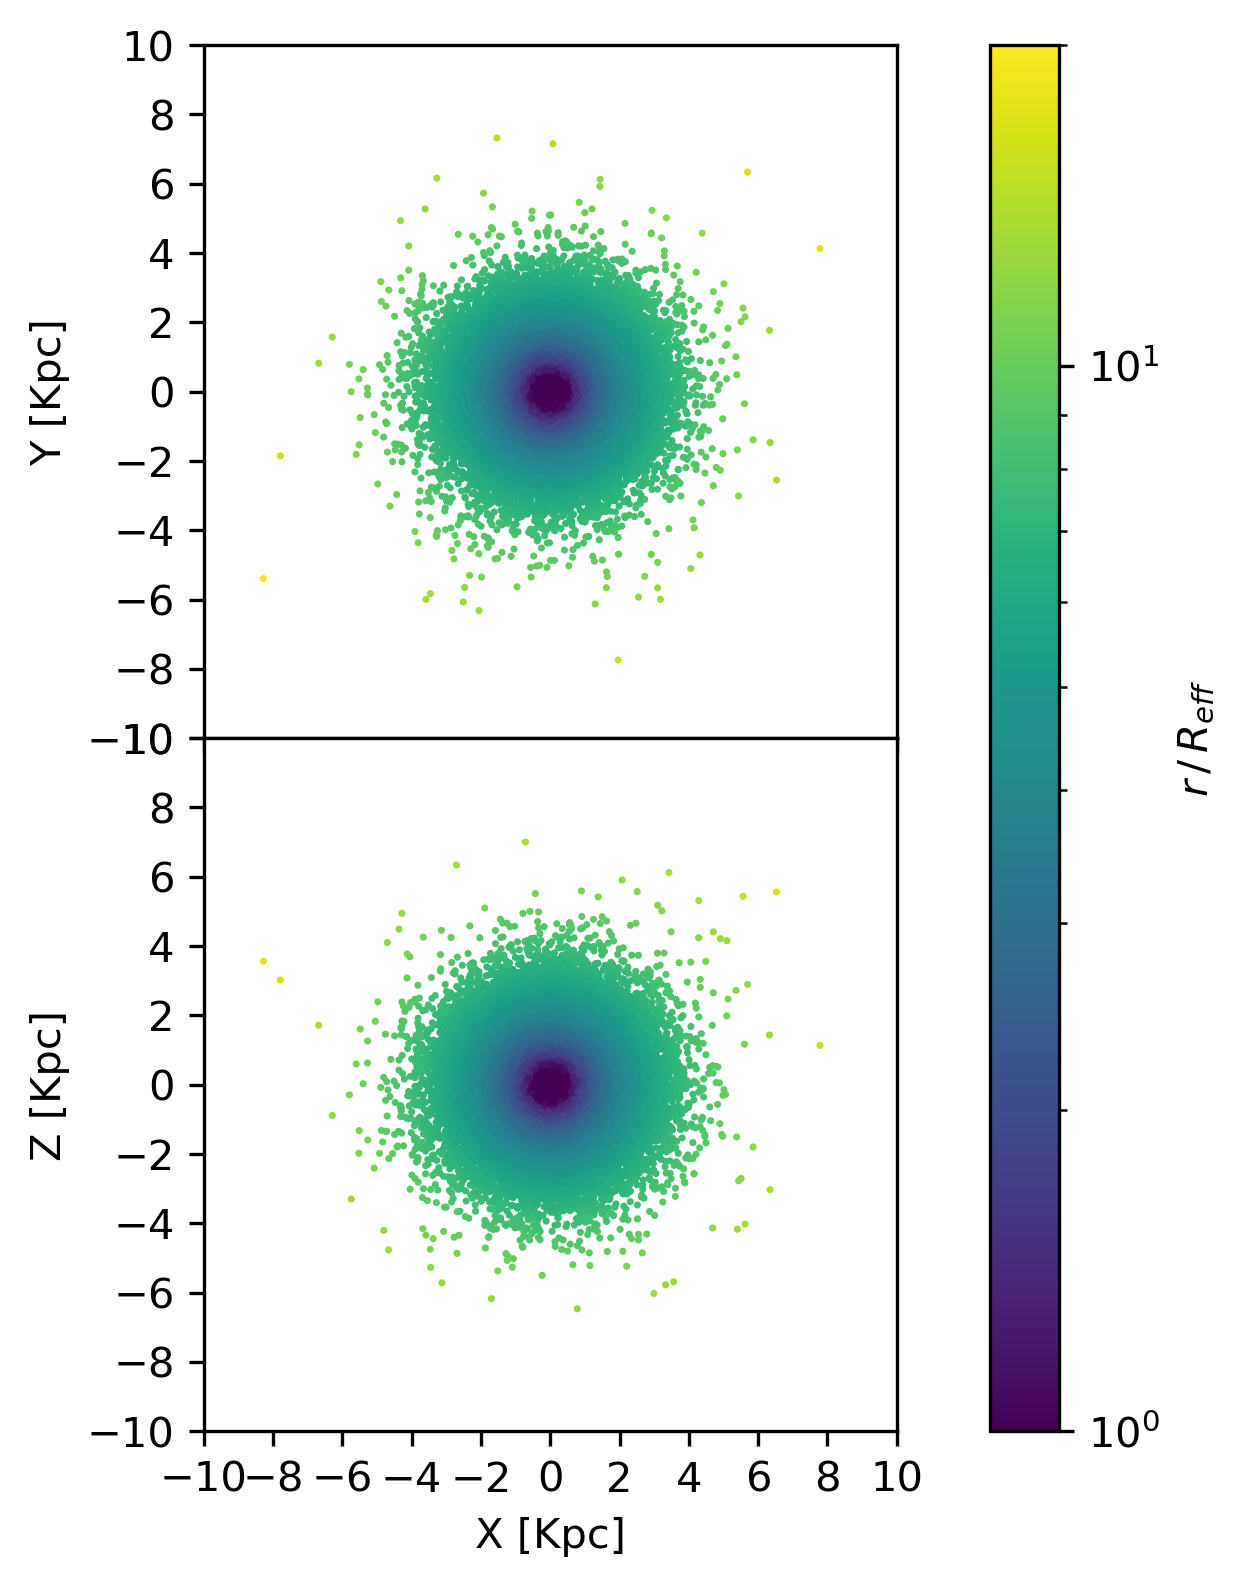
\includegraphics[width=\linewidth]{NGC205_bulge_scatter_XY_XZ.png}
        \caption{A}
    \end{subfigure}
    \hfill
    \begin{subfigure}{0.3\textwidth}
        \centering
        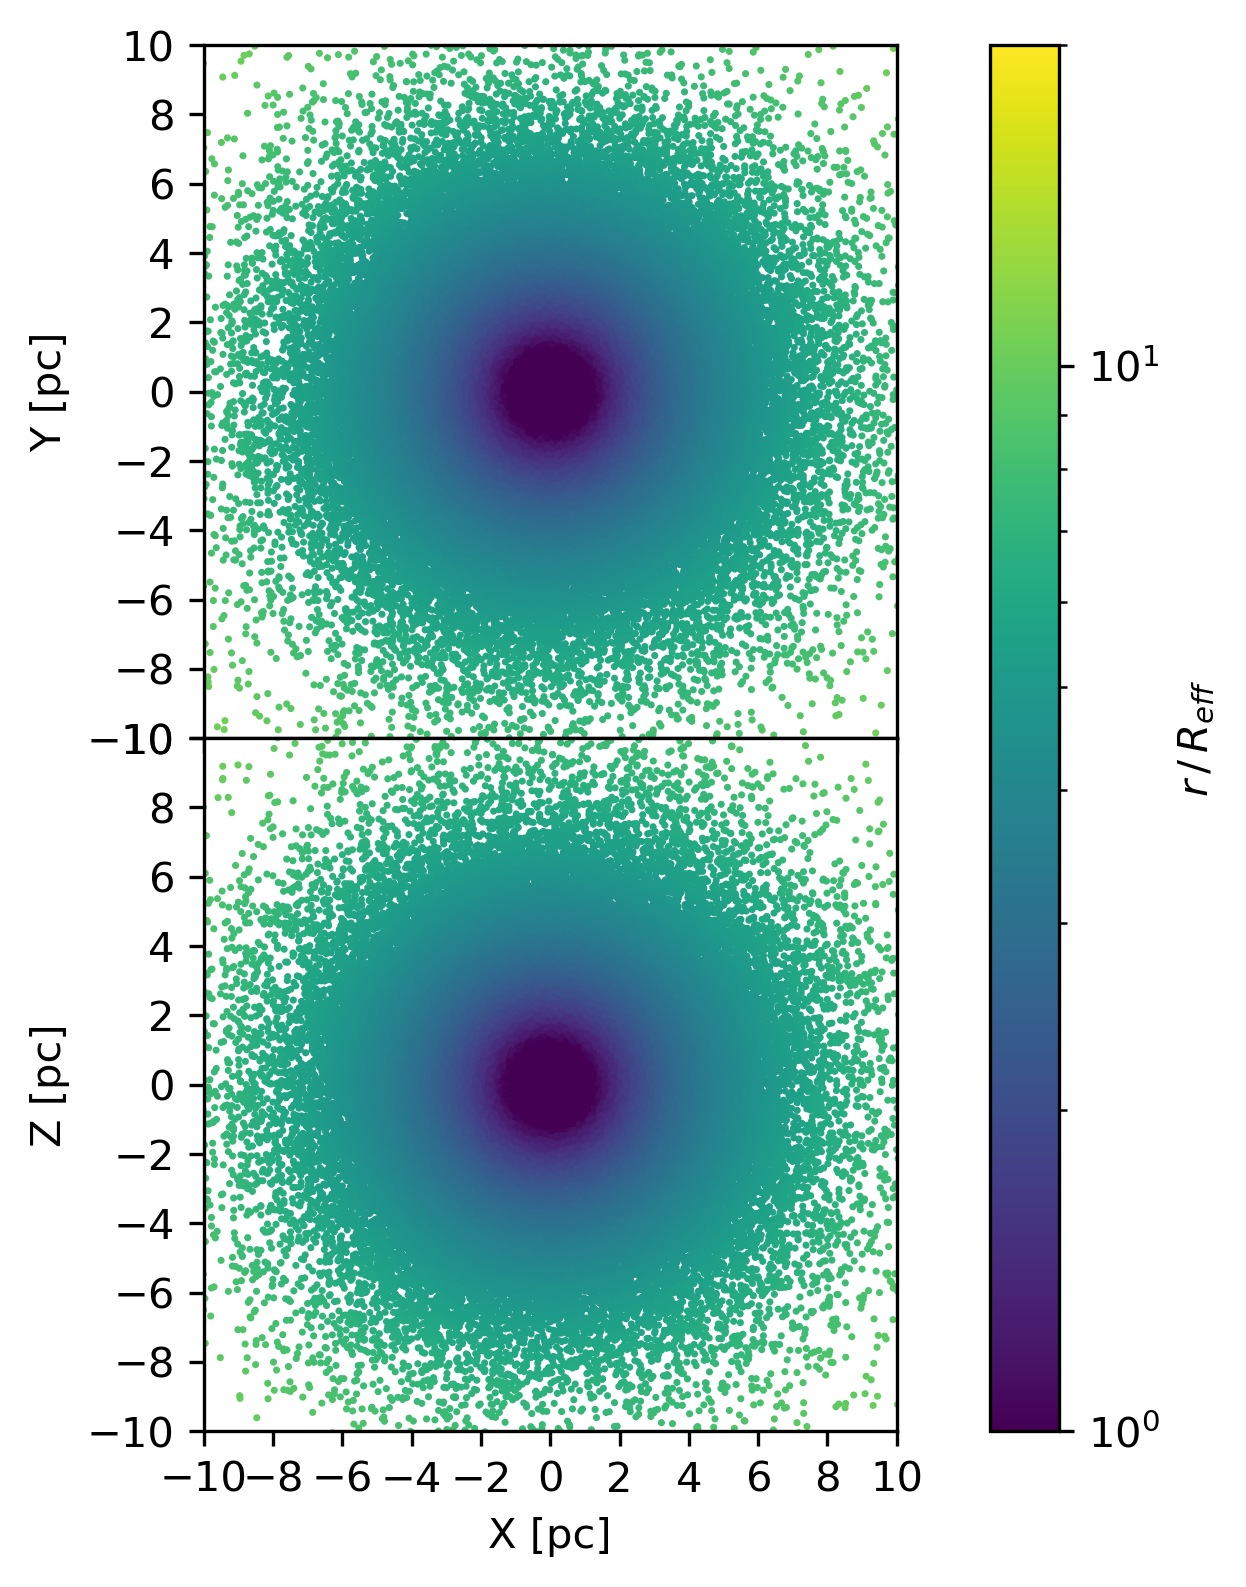
\includegraphics[width=\linewidth]{NGC205_NSC_scatter_XY_XZ.png}
        \caption{B}
    \end{subfigure}
    \hfill
    \begin{subfigure}{0.3\textwidth}
        \centering
        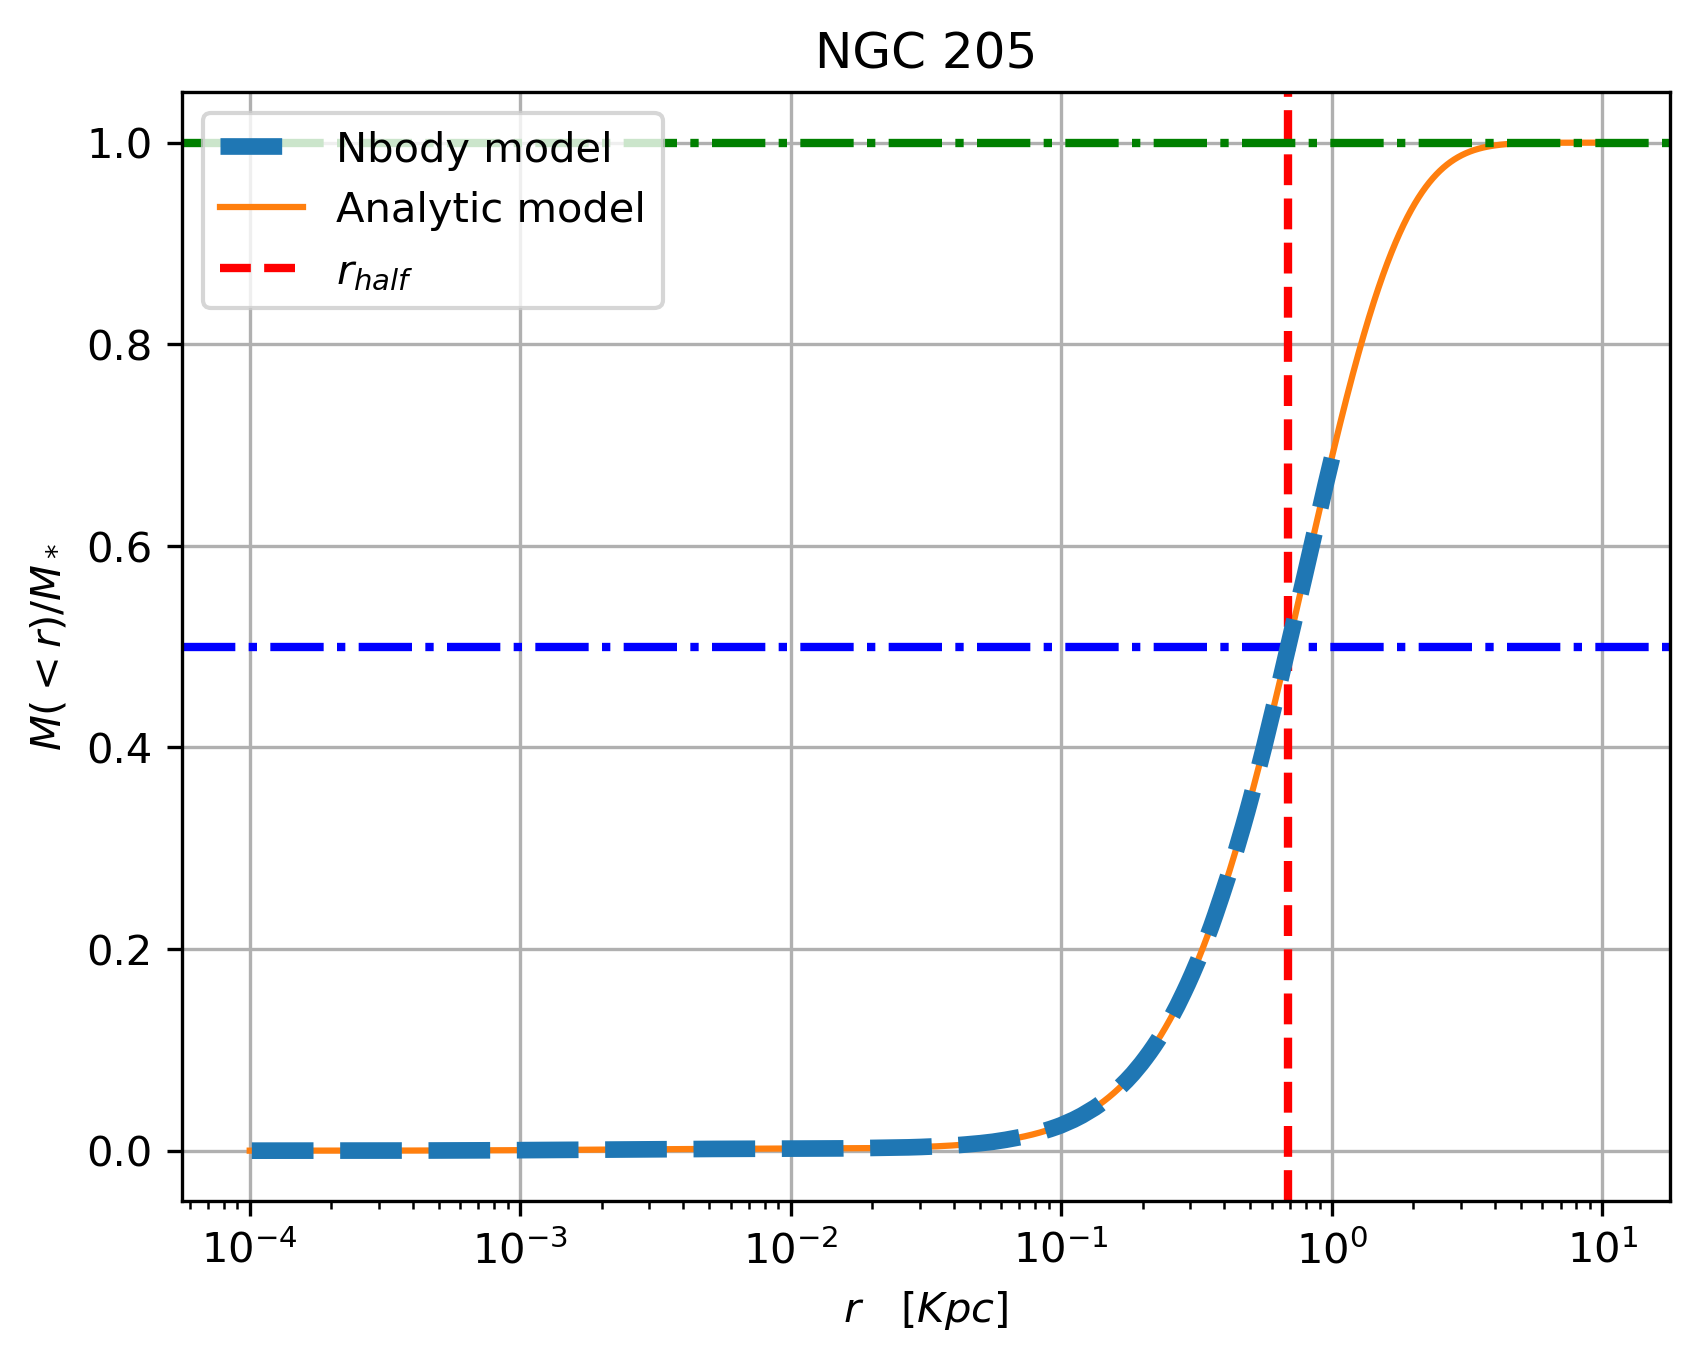
\includegraphics[width=\linewidth]{NGC205_halfmass.png}
        \caption{C}
    \end{subfigure}

    \caption{aaa}
    \label{3 NGC205_velocity_hist}
\end{figure}







\begin{figure}[h]
\centering
 \begin{subfigure}{0.3\textwidth}
        \centering
        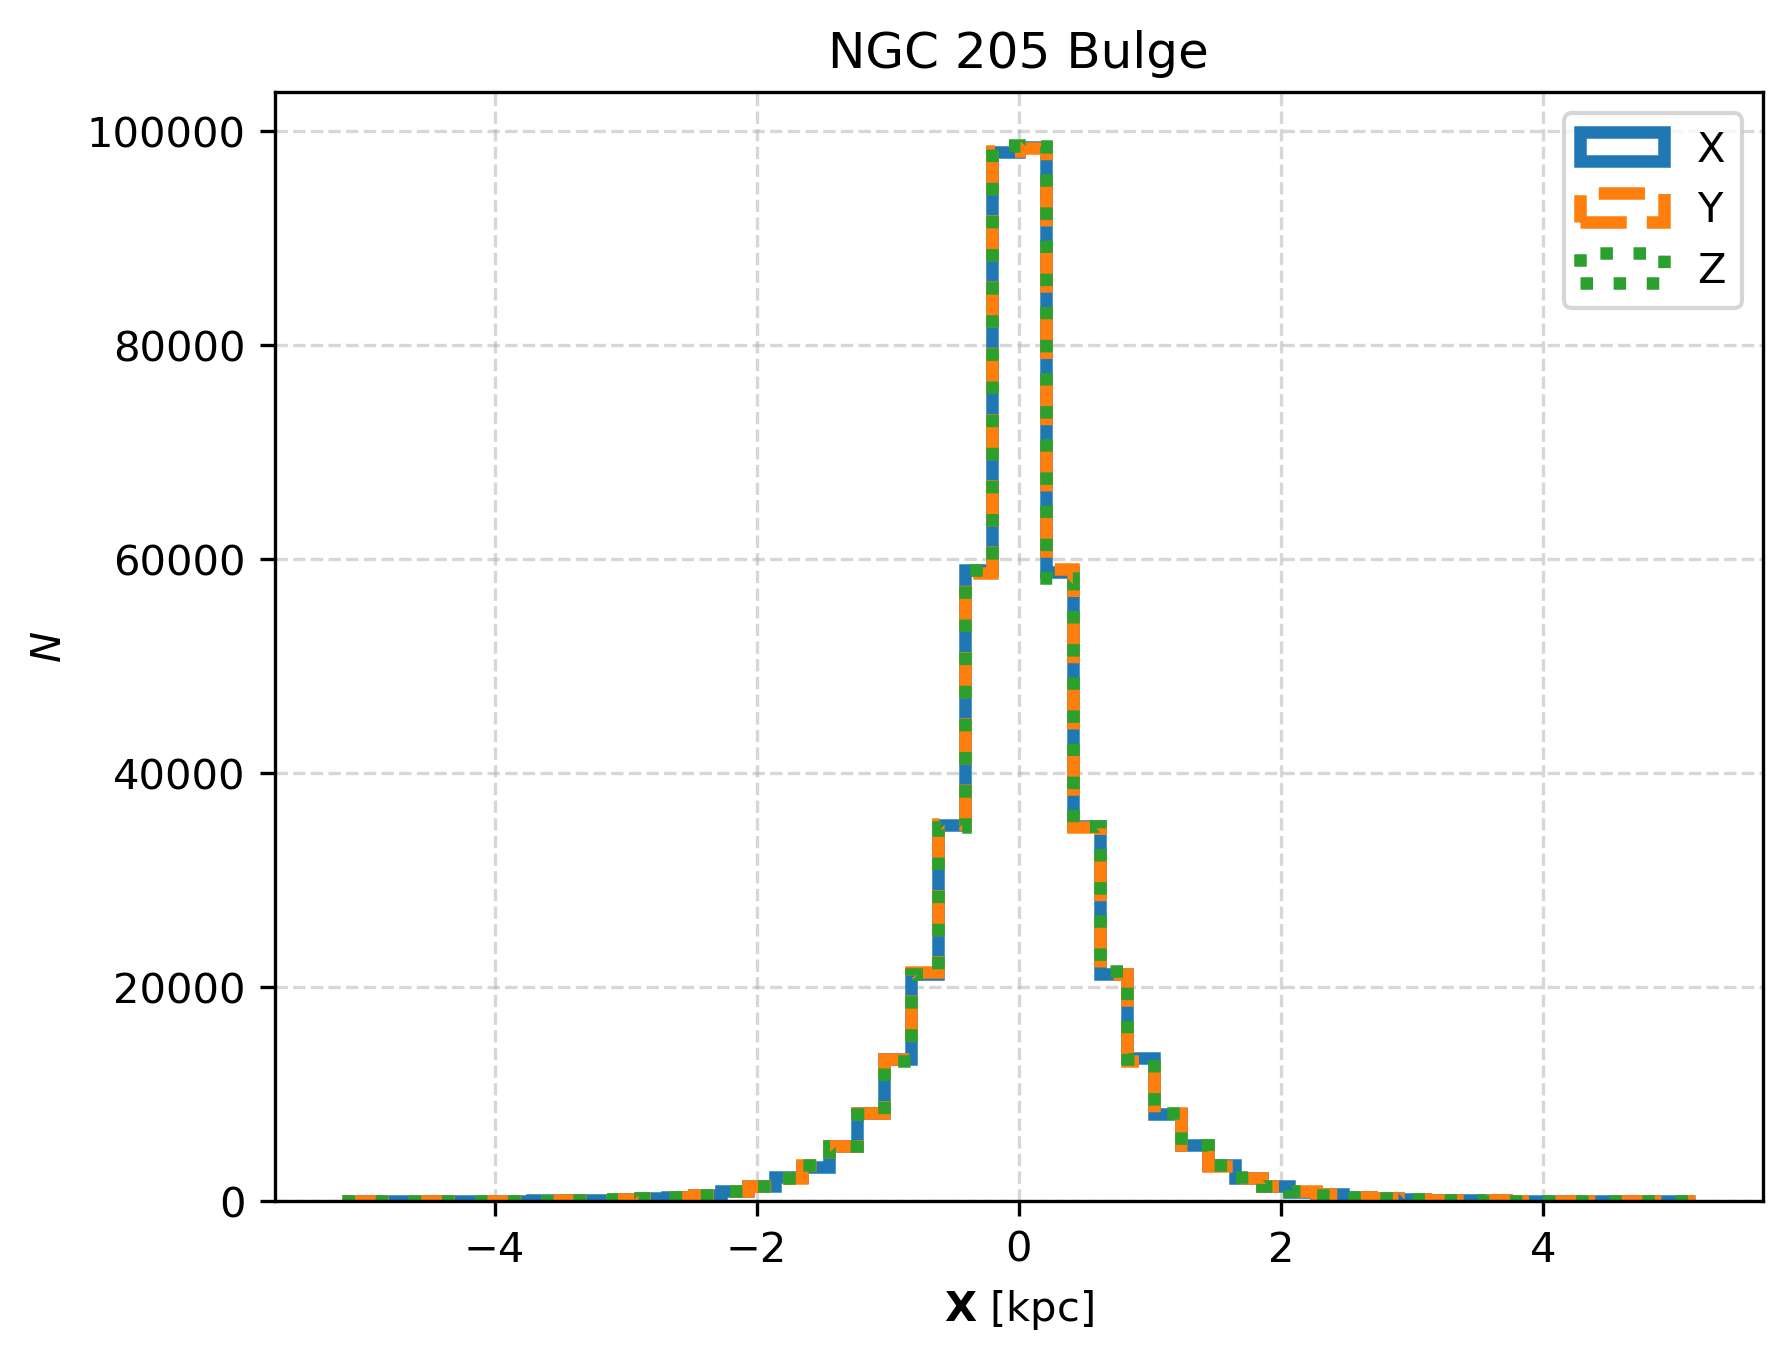
\includegraphics[width=\linewidth]{NGC205_bulge_space_hist.png}
        \caption{A}
    \end{subfigure}
    \hfill
    \begin{subfigure}{0.3\textwidth}
        \centering
        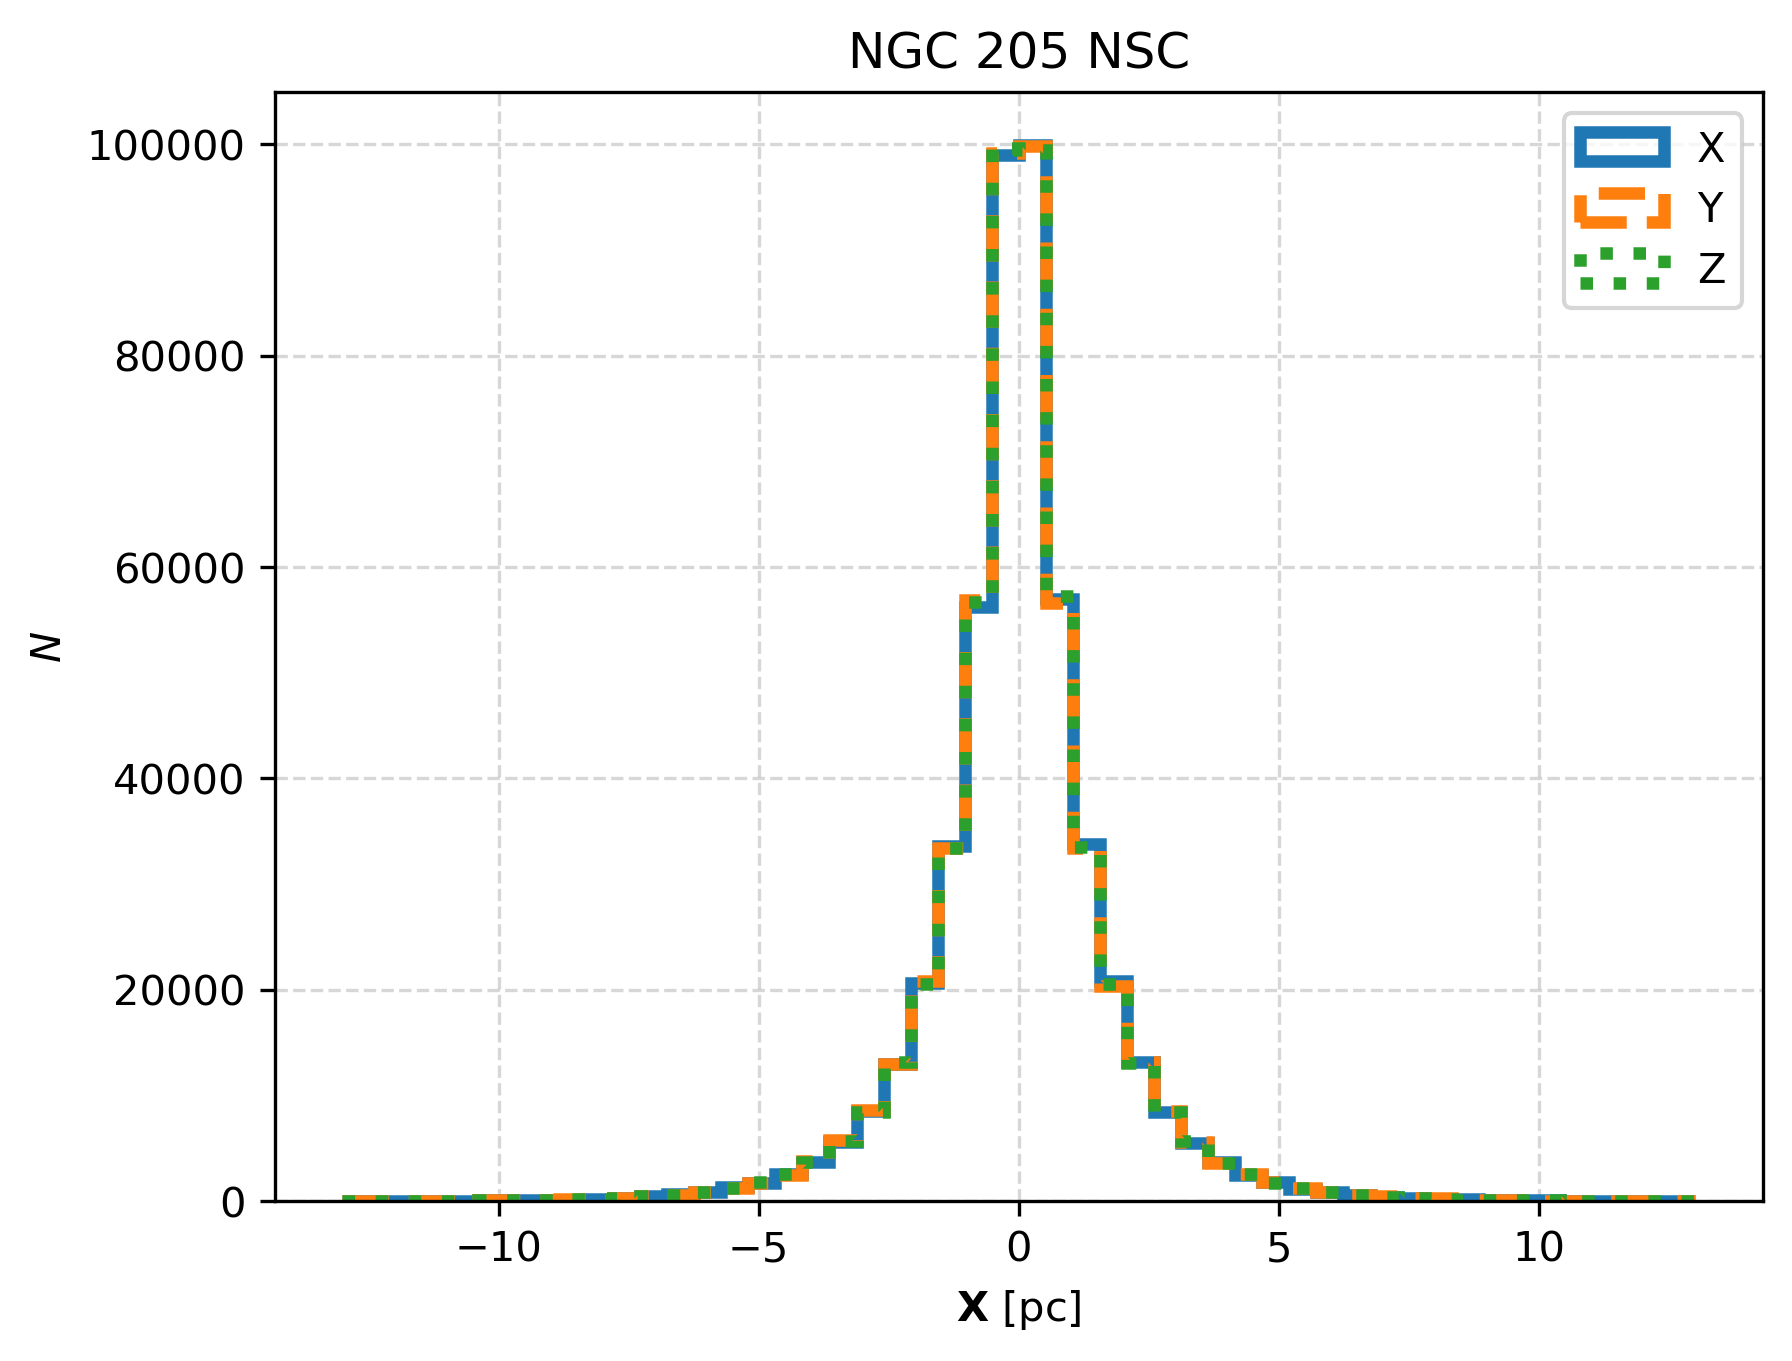
\includegraphics[width=\linewidth]{NGC205_NSC_space_hist.png}
        \caption{B}
    \end{subfigure}
    \hfill
    \begin{subfigure}{0.3\textwidth}
        \centering
        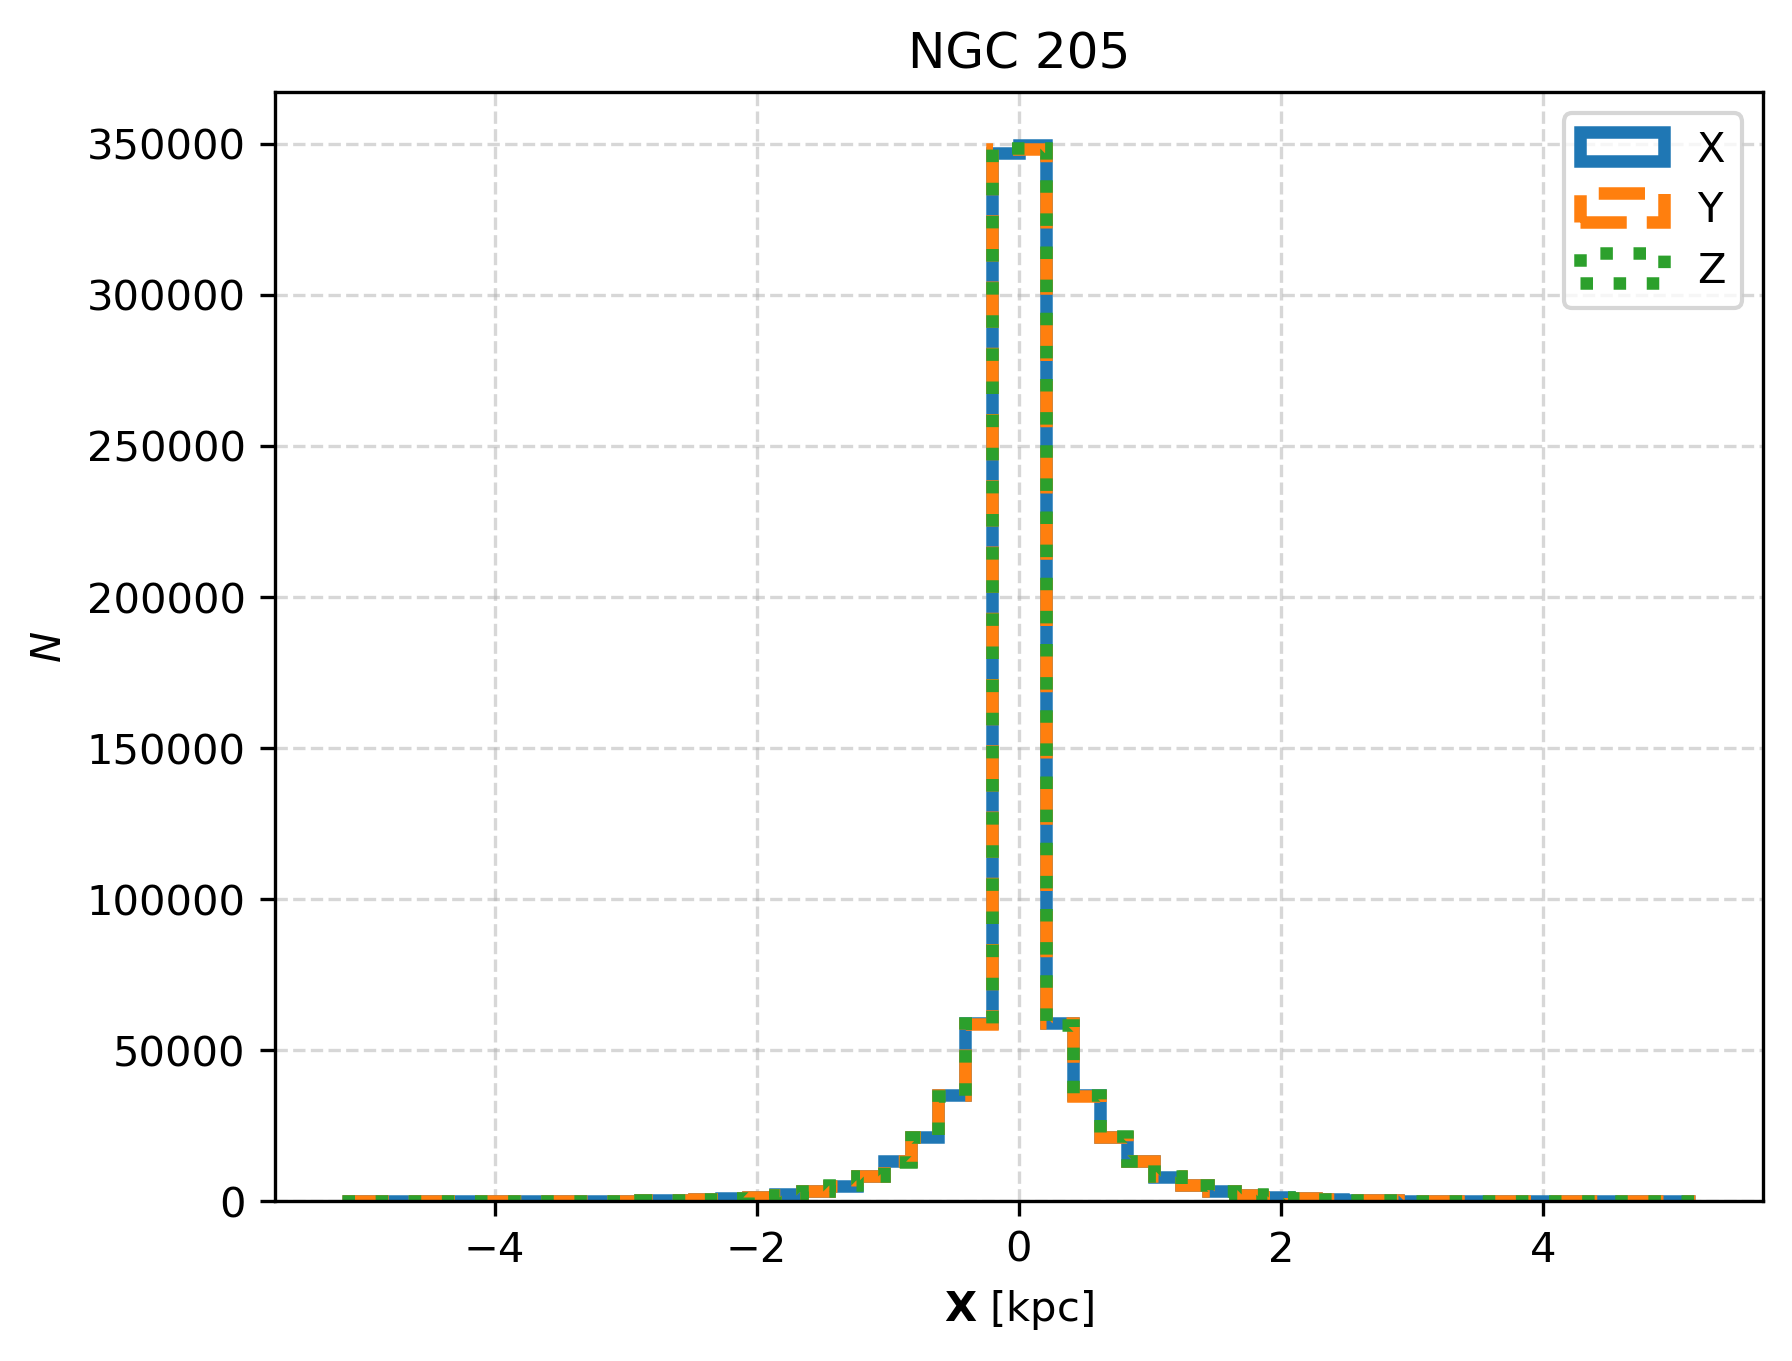
\includegraphics[width=\linewidth]{NGC205_space_hist.png}
        \caption{C}
    \end{subfigure}
    
    \caption{aaa}
    \label{3 NGC205_space_hist}
\end{figure}

\begin{figure}[h]
\centering
 \begin{subfigure}{0.3\textwidth}
        \centering
        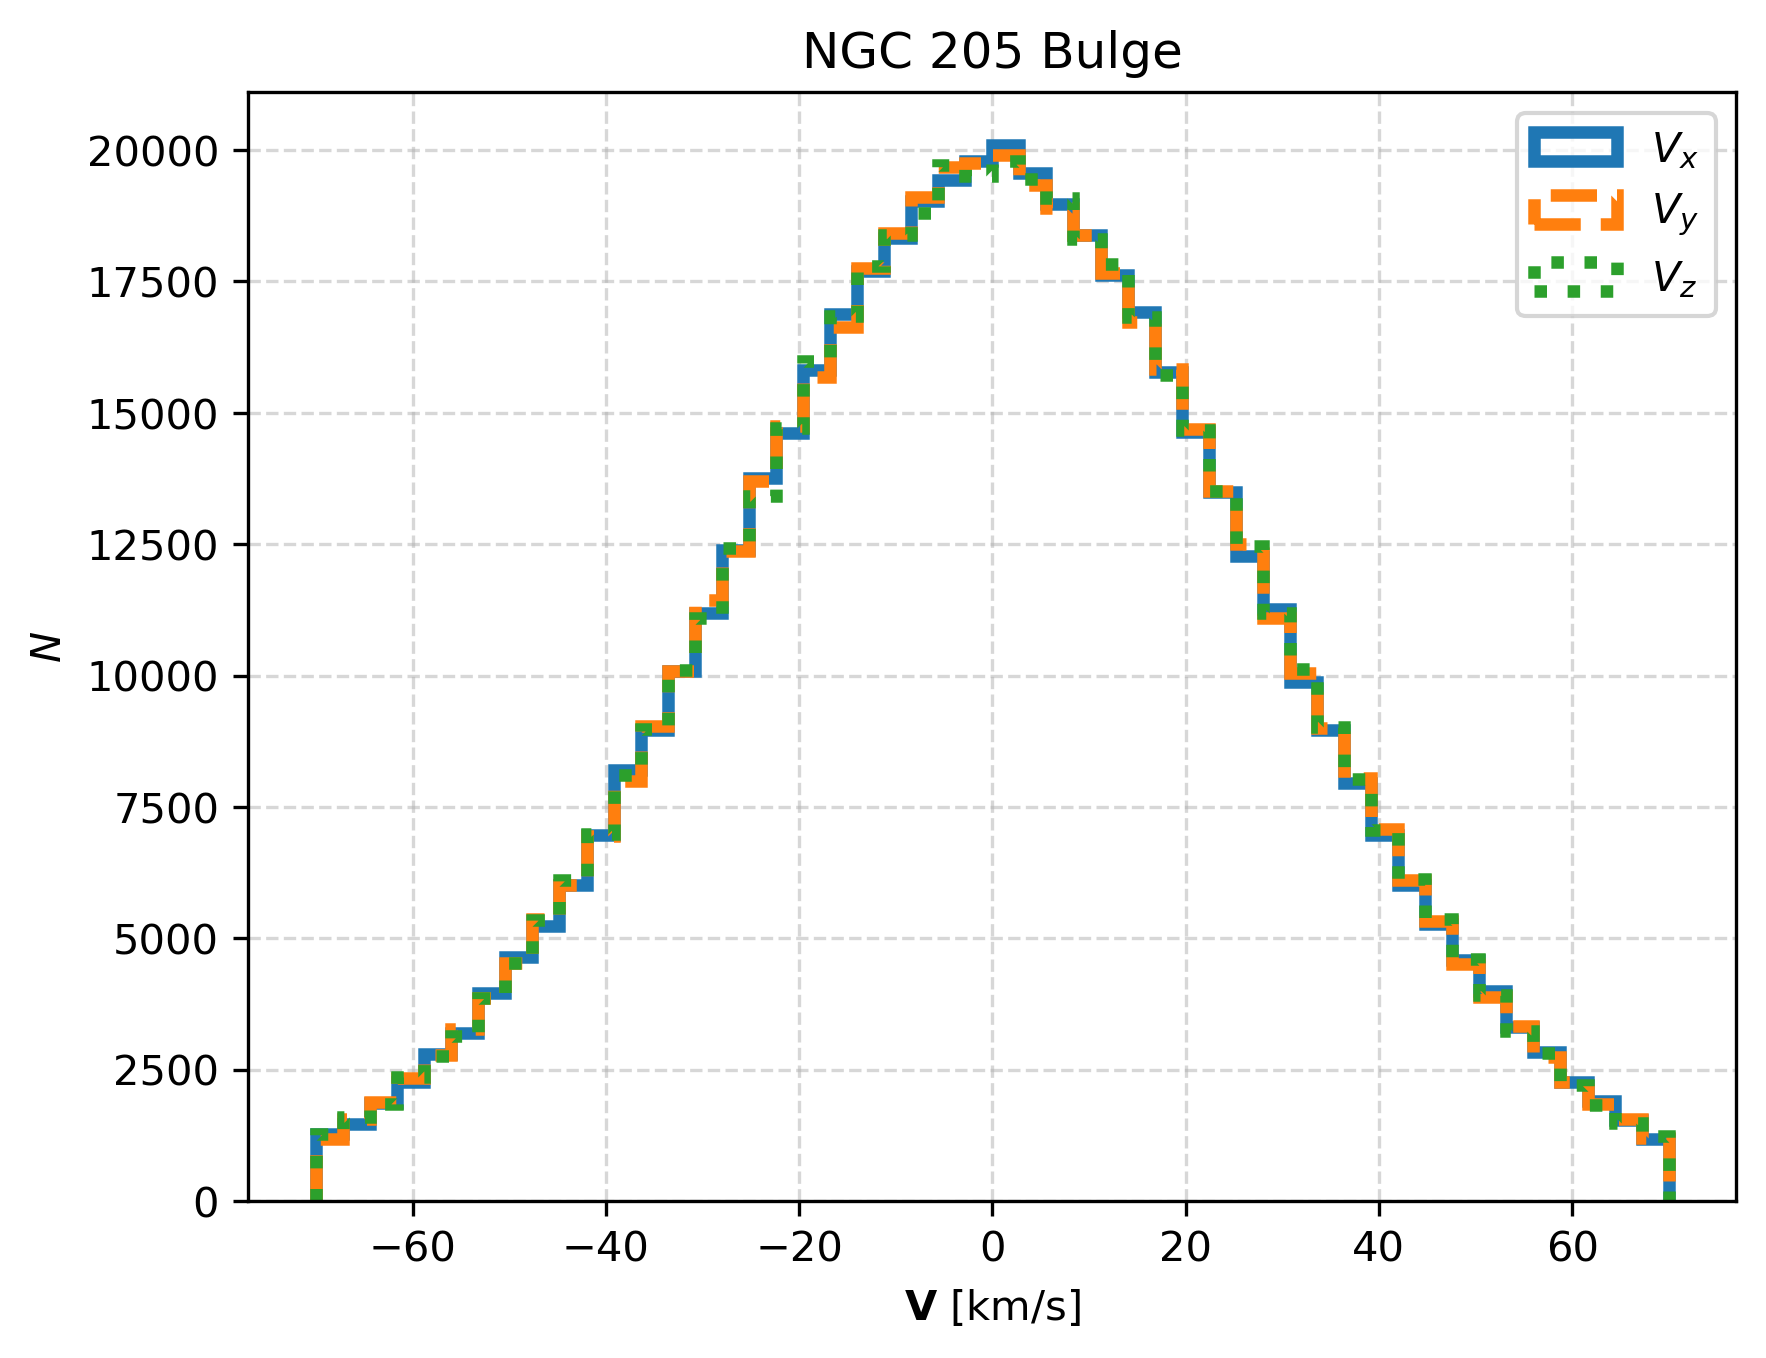
\includegraphics[width=\linewidth]{NGC205_bulge_velocity_hist.png}
        \caption{A}
    \end{subfigure}
    \hfill
    \begin{subfigure}{0.3\textwidth}
        \centering
        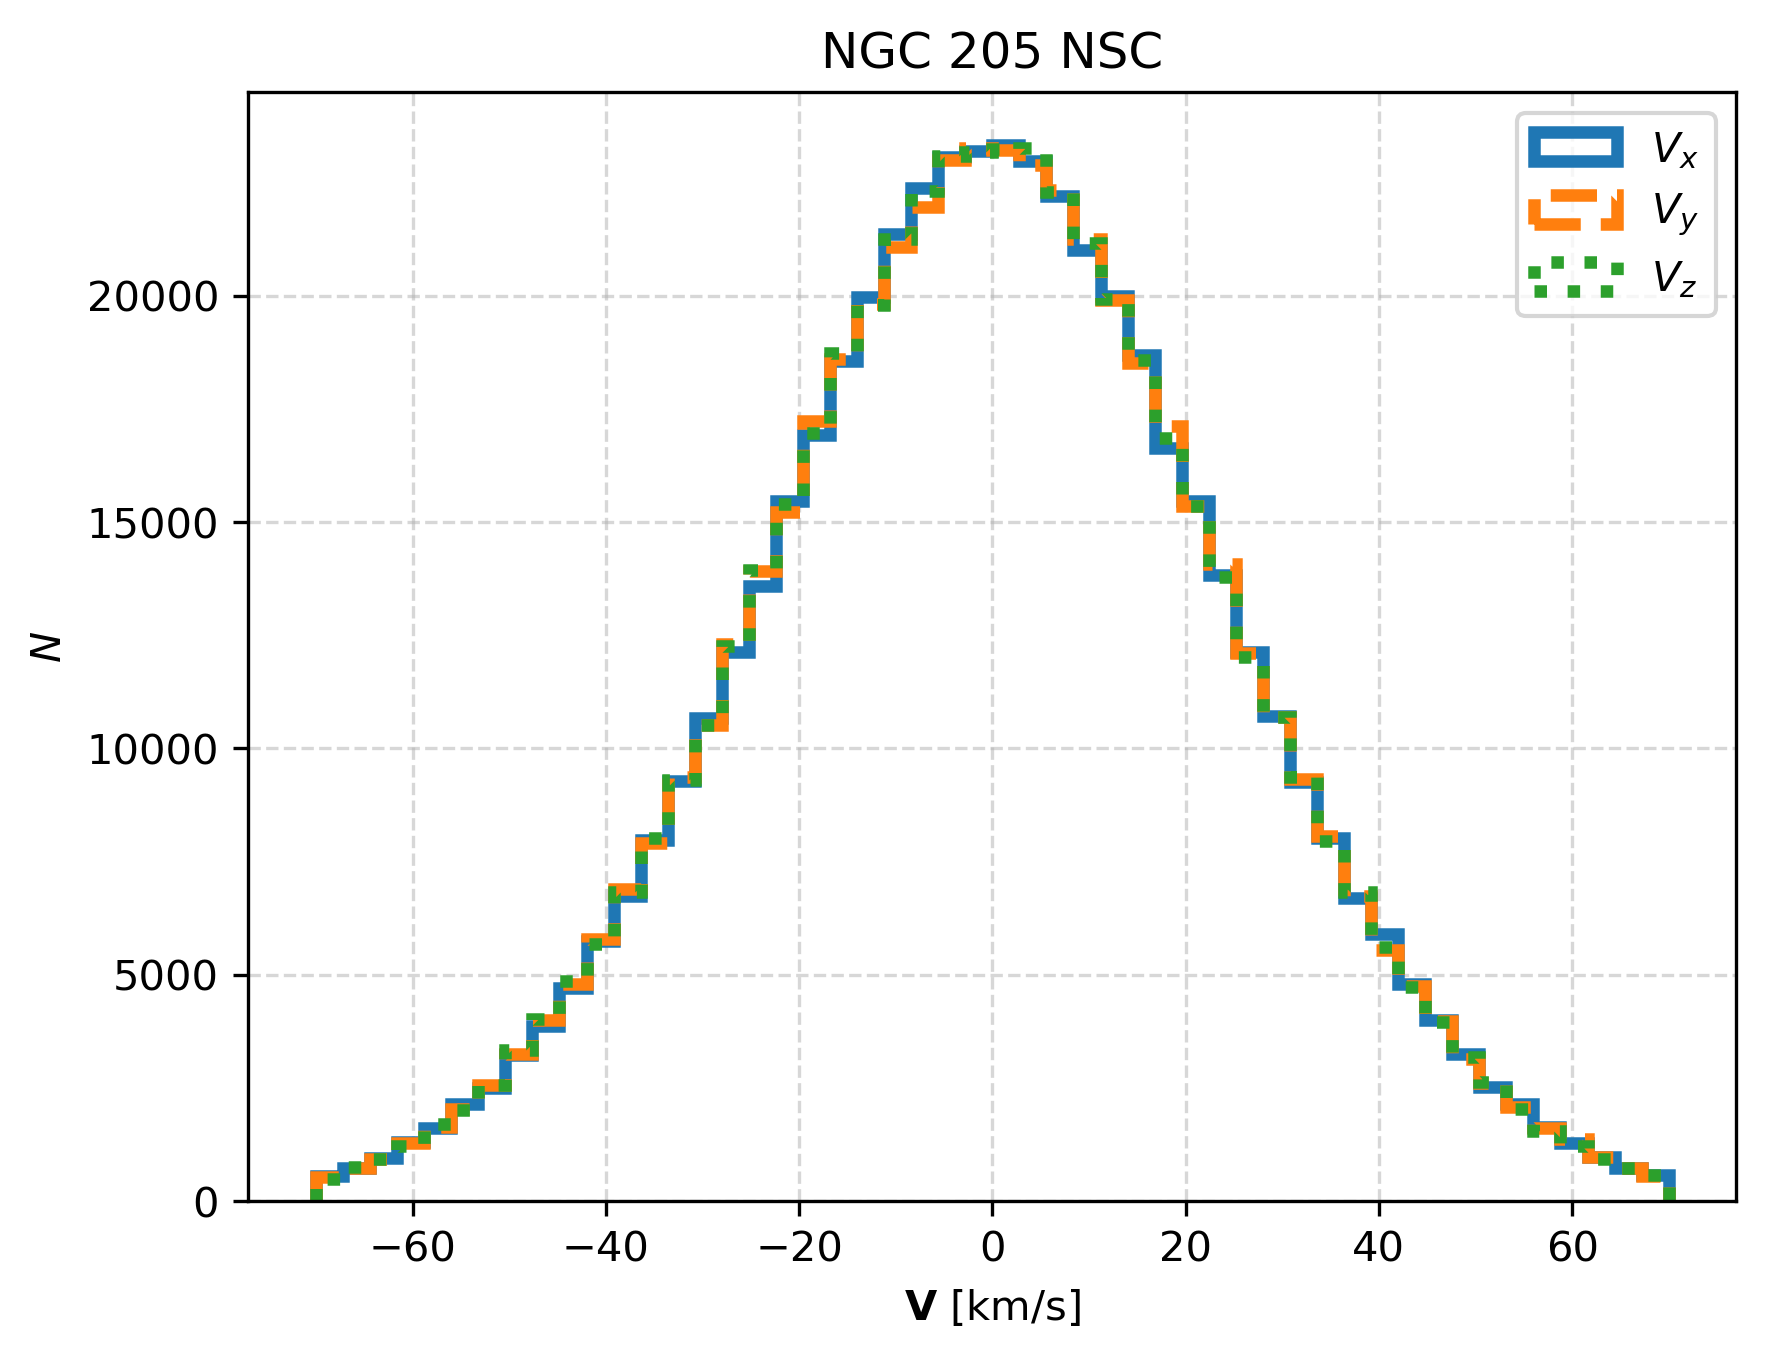
\includegraphics[width=\linewidth]{NGC205_NSC_velocity_hist.png}
        \caption{B}
    \end{subfigure}
    \hfill
    \begin{subfigure}{0.3\textwidth}
        \centering
        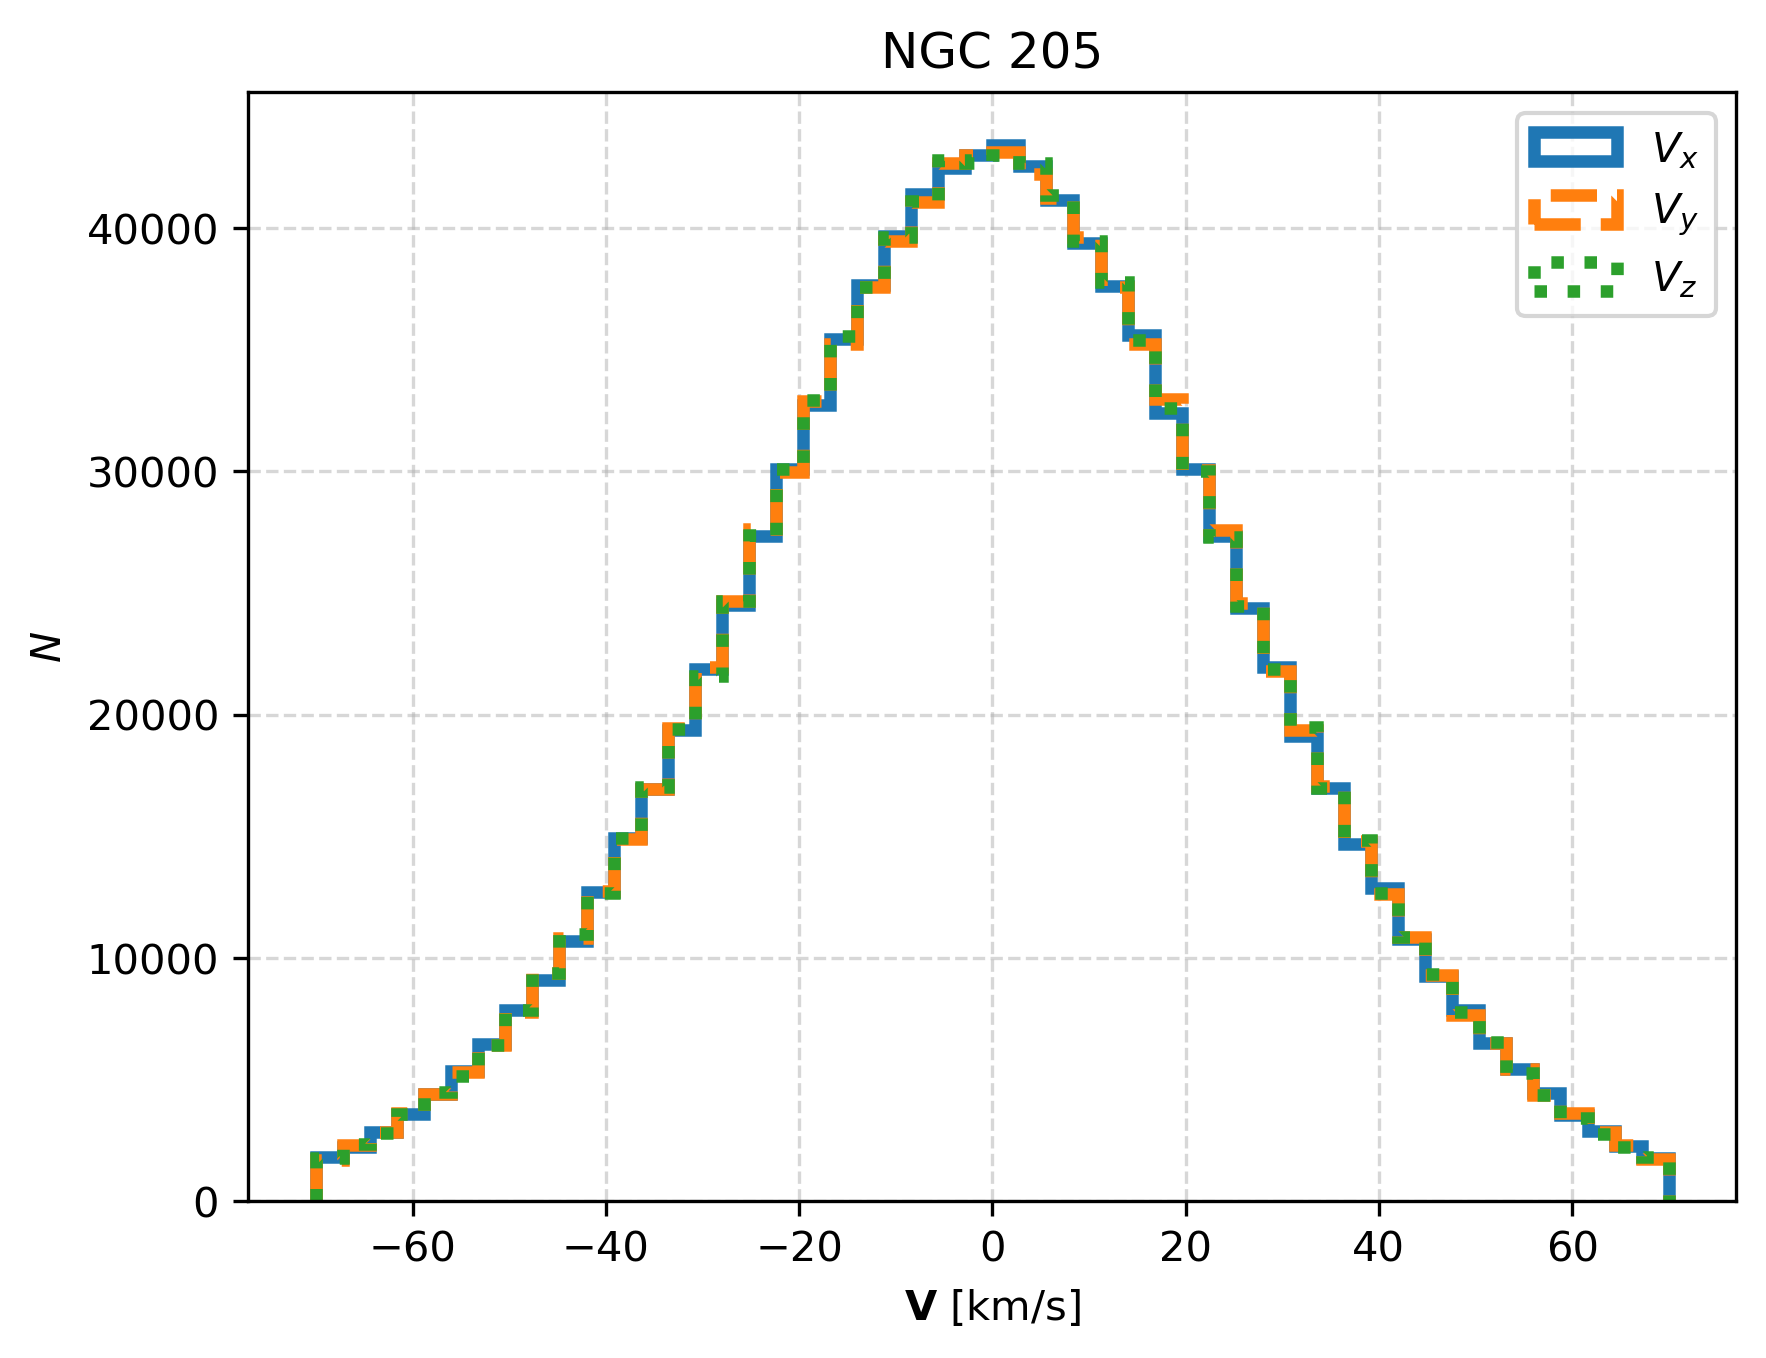
\includegraphics[width=\linewidth]{NGC205_velocity_hist.png}
        \caption{C}
    \end{subfigure}
    
    \caption{aaa}
    \label{3 NGC205_velocity_hist}
\end{figure}

\begin{figure}[h]
\centering
 \begin{subfigure}{0.3\textwidth}
        \centering
        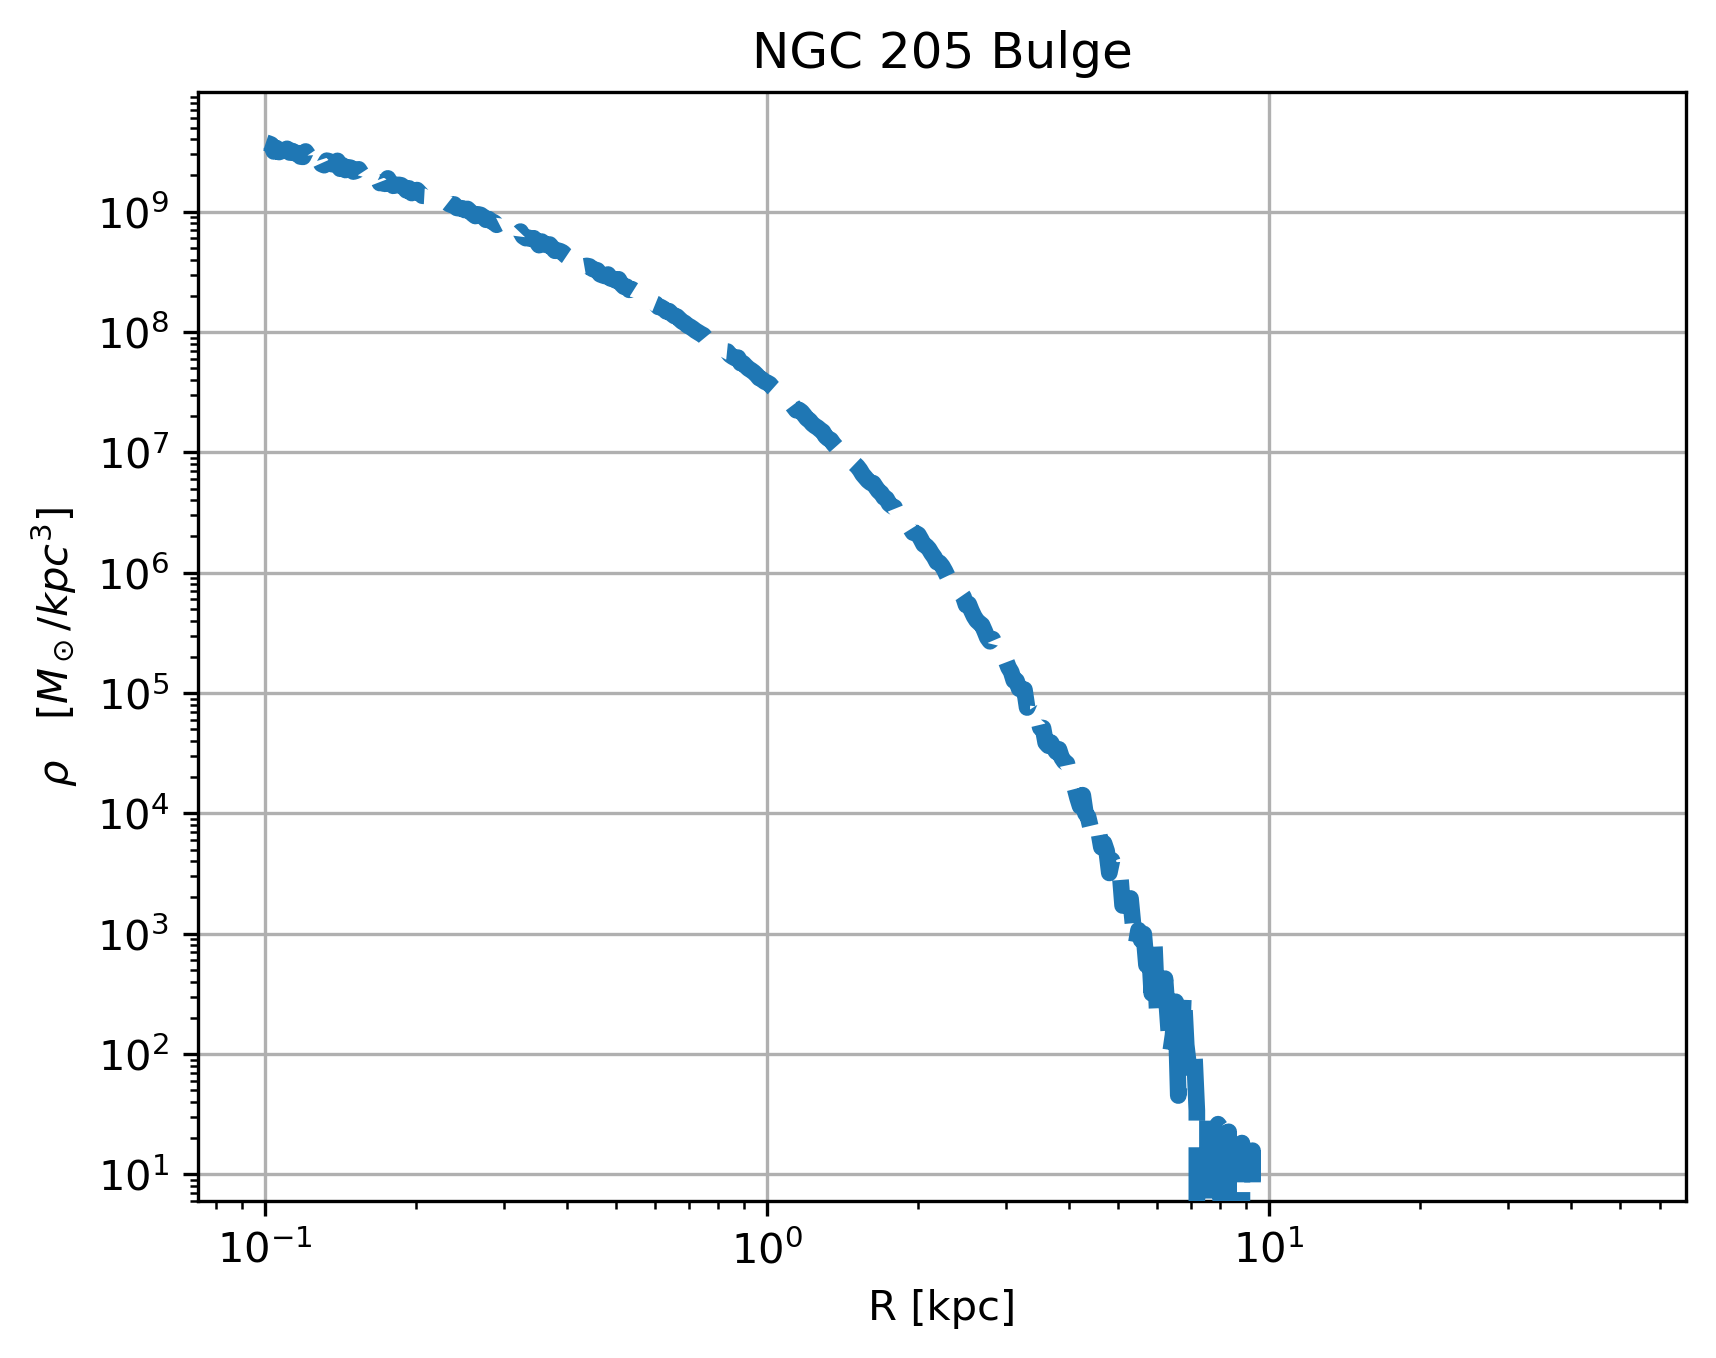
\includegraphics[width=\linewidth]{NGC205_bulge_density_Nbody.png}
        \caption{A}
    \end{subfigure}
    \hfill
    \begin{subfigure}{0.3\textwidth}
        \centering
        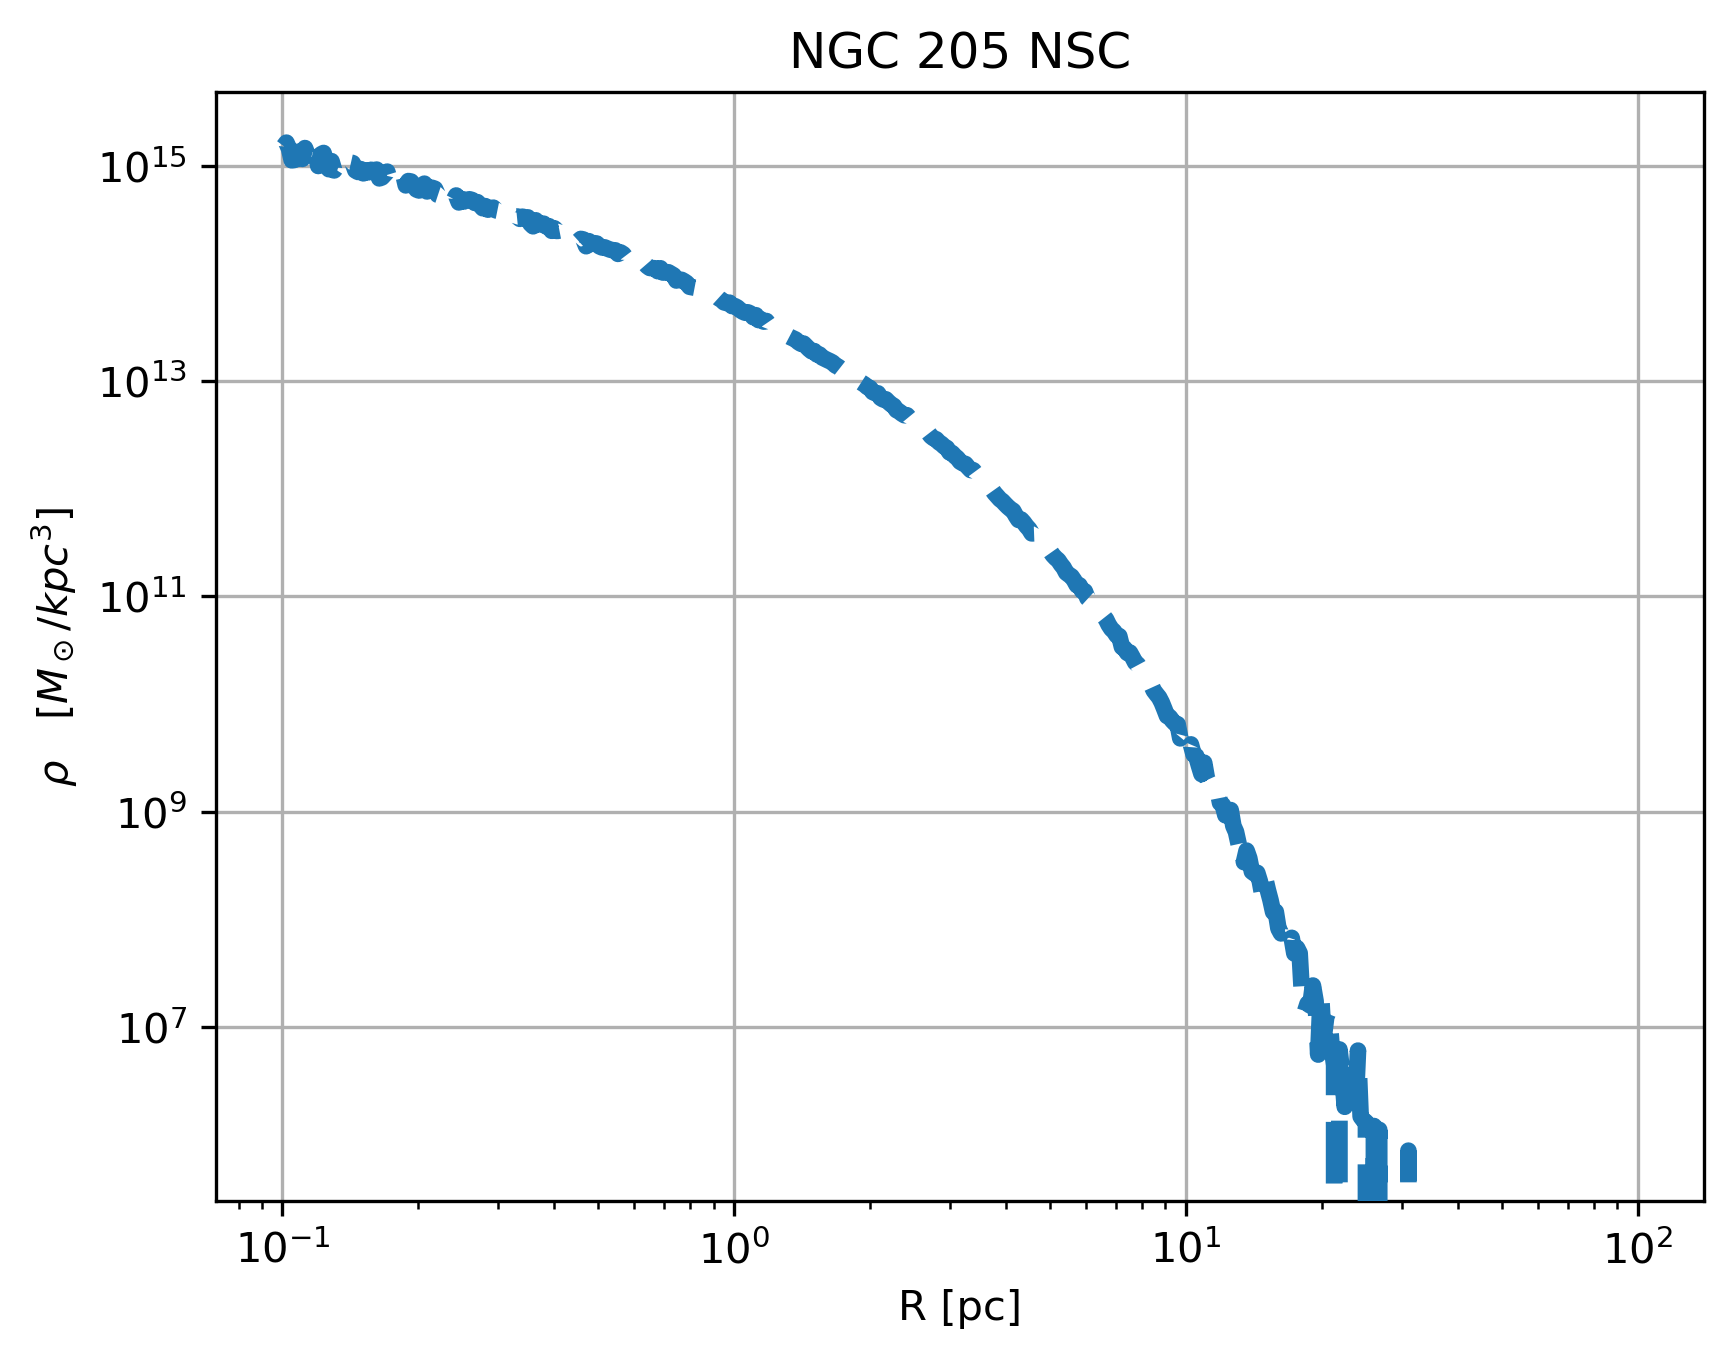
\includegraphics[width=\linewidth]{NGC205_NSC_density_Nbody.png}
        \caption{B}
    \end{subfigure}
    \hfill
    \begin{subfigure}{0.3\textwidth}
        \centering
        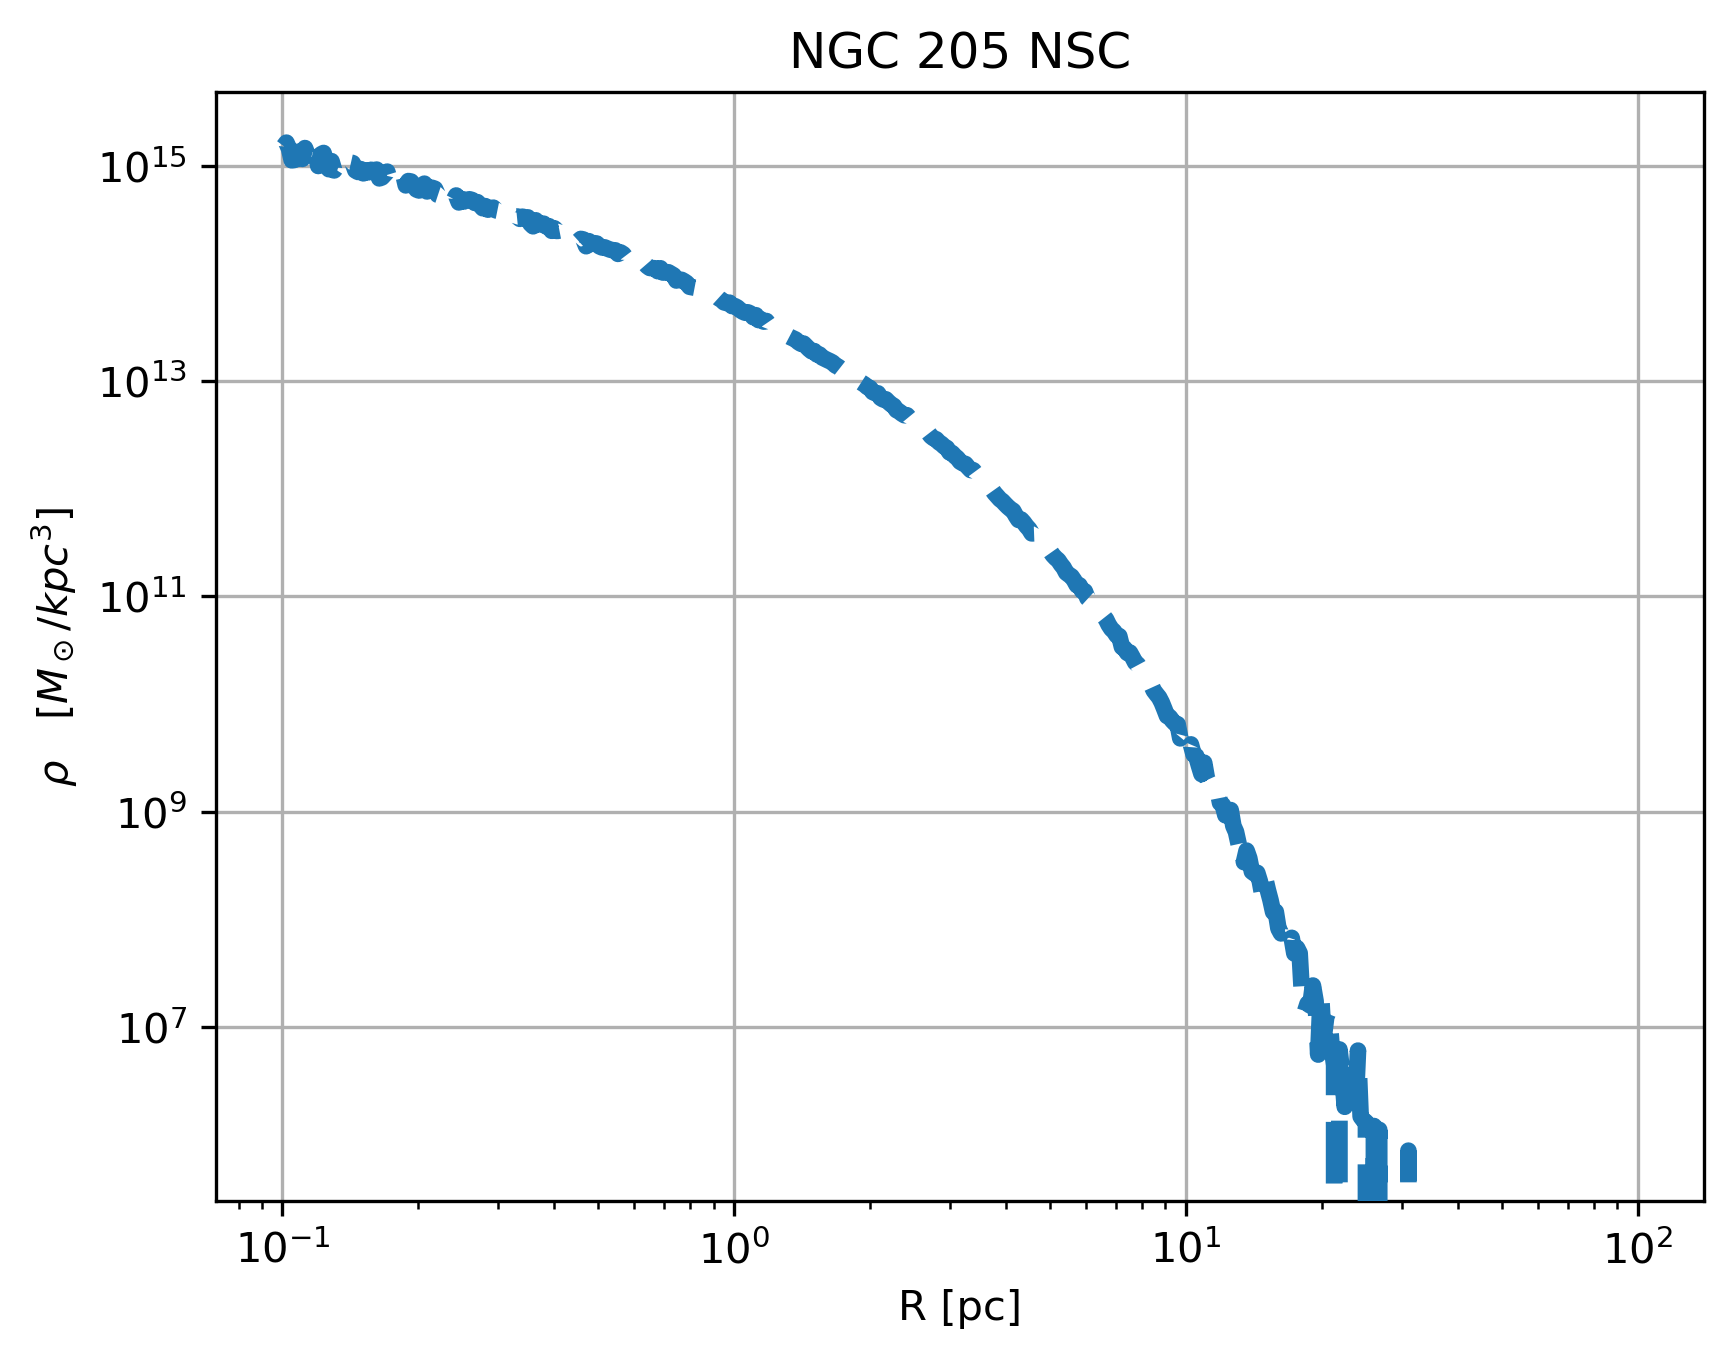
\includegraphics[width=\linewidth]{NGC205_NSC_density_Nbody.png}
        \caption{C}
    \end{subfigure}
    
    \caption{aaa}
    \label{3 NGC205_density_Nbody}
\end{figure}

\begin{figure}[h]
\centering

\begin{subfigure}{0.45\textwidth}
\centering
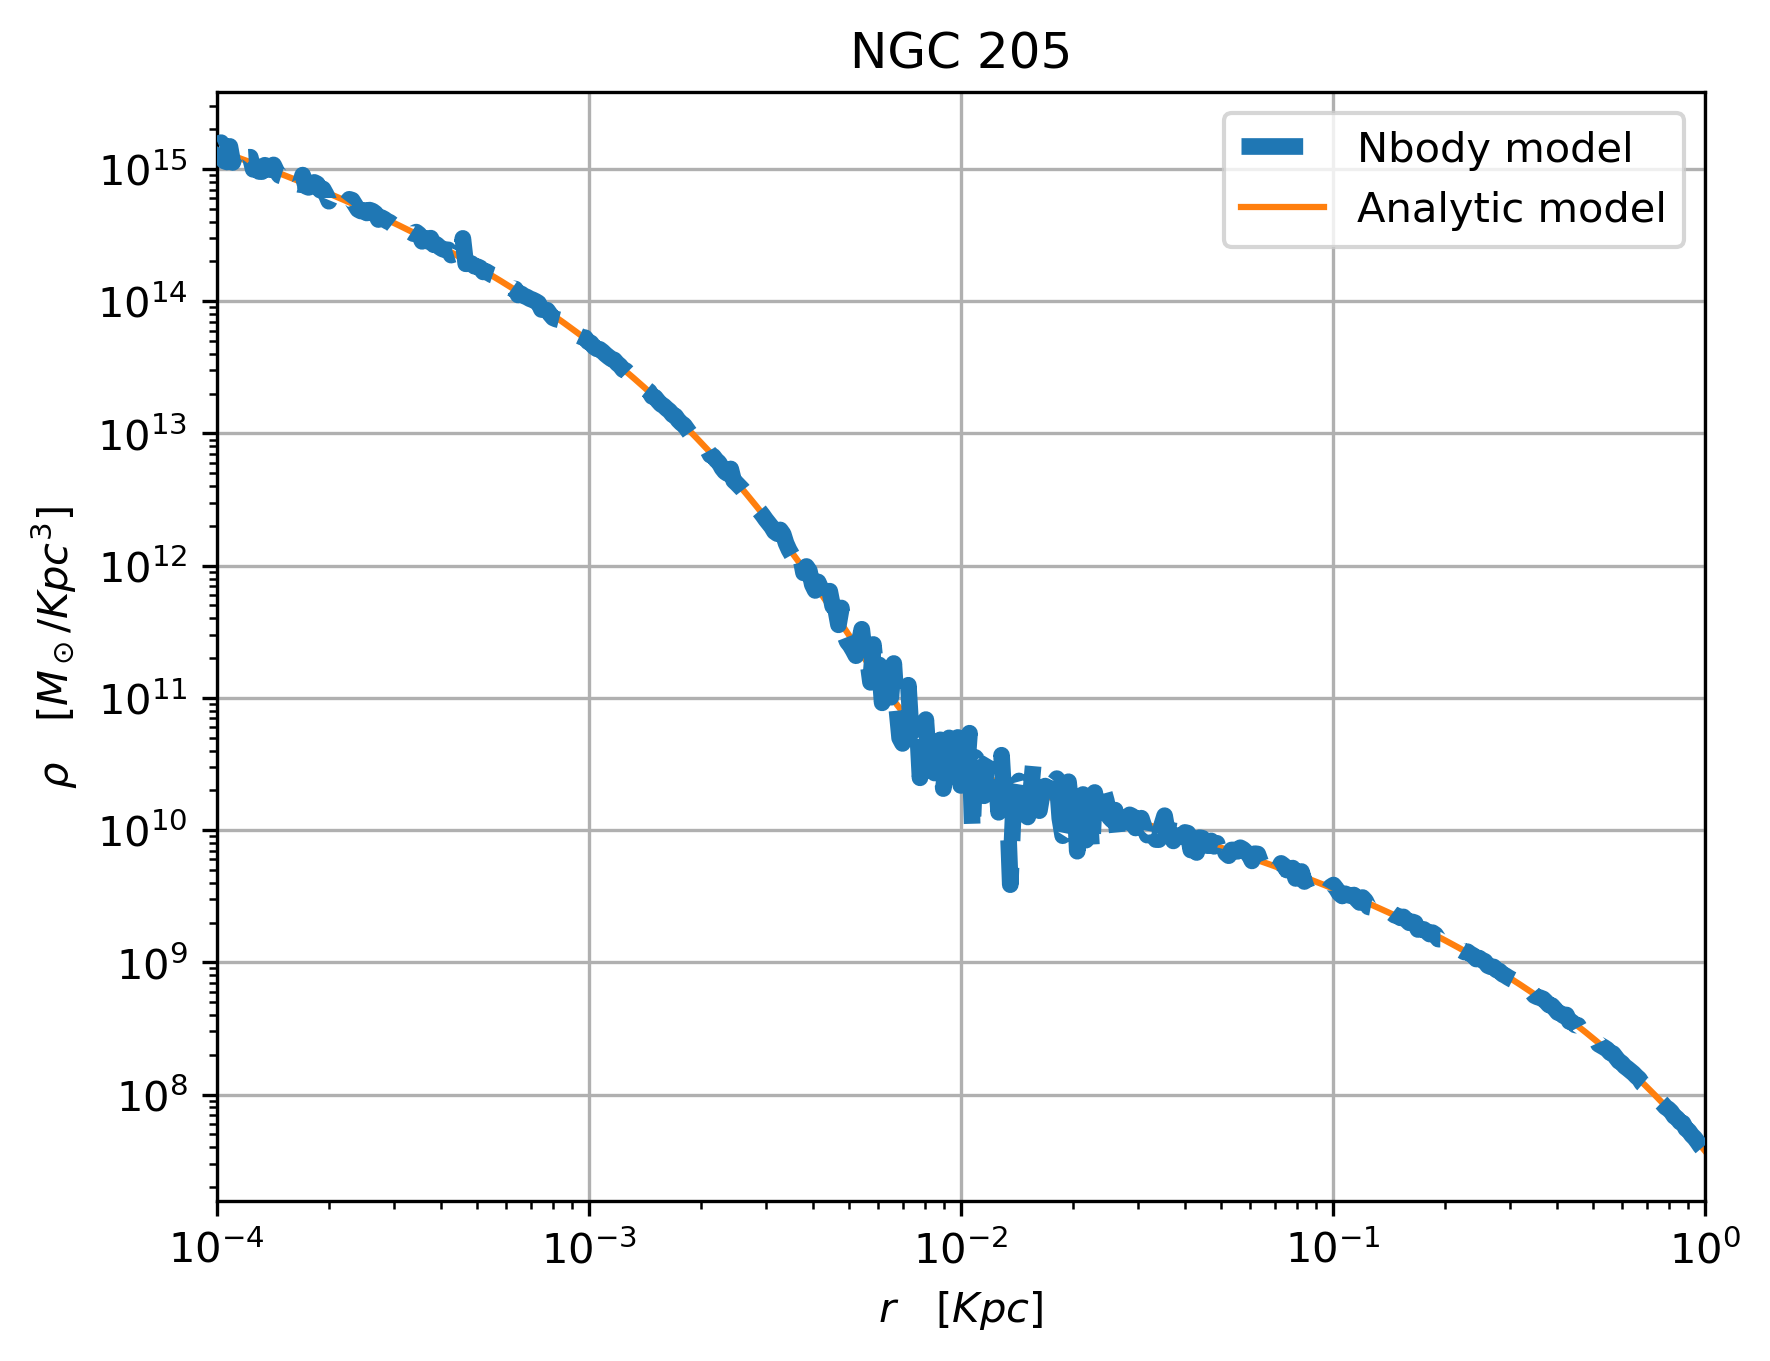
\includegraphics[width=\linewidth]{NGC205_density_Nbody_vs_analytic.png}
\caption{A}
\end{subfigure}
\hfill
\begin{subfigure}{0.45\textwidth}
\centering
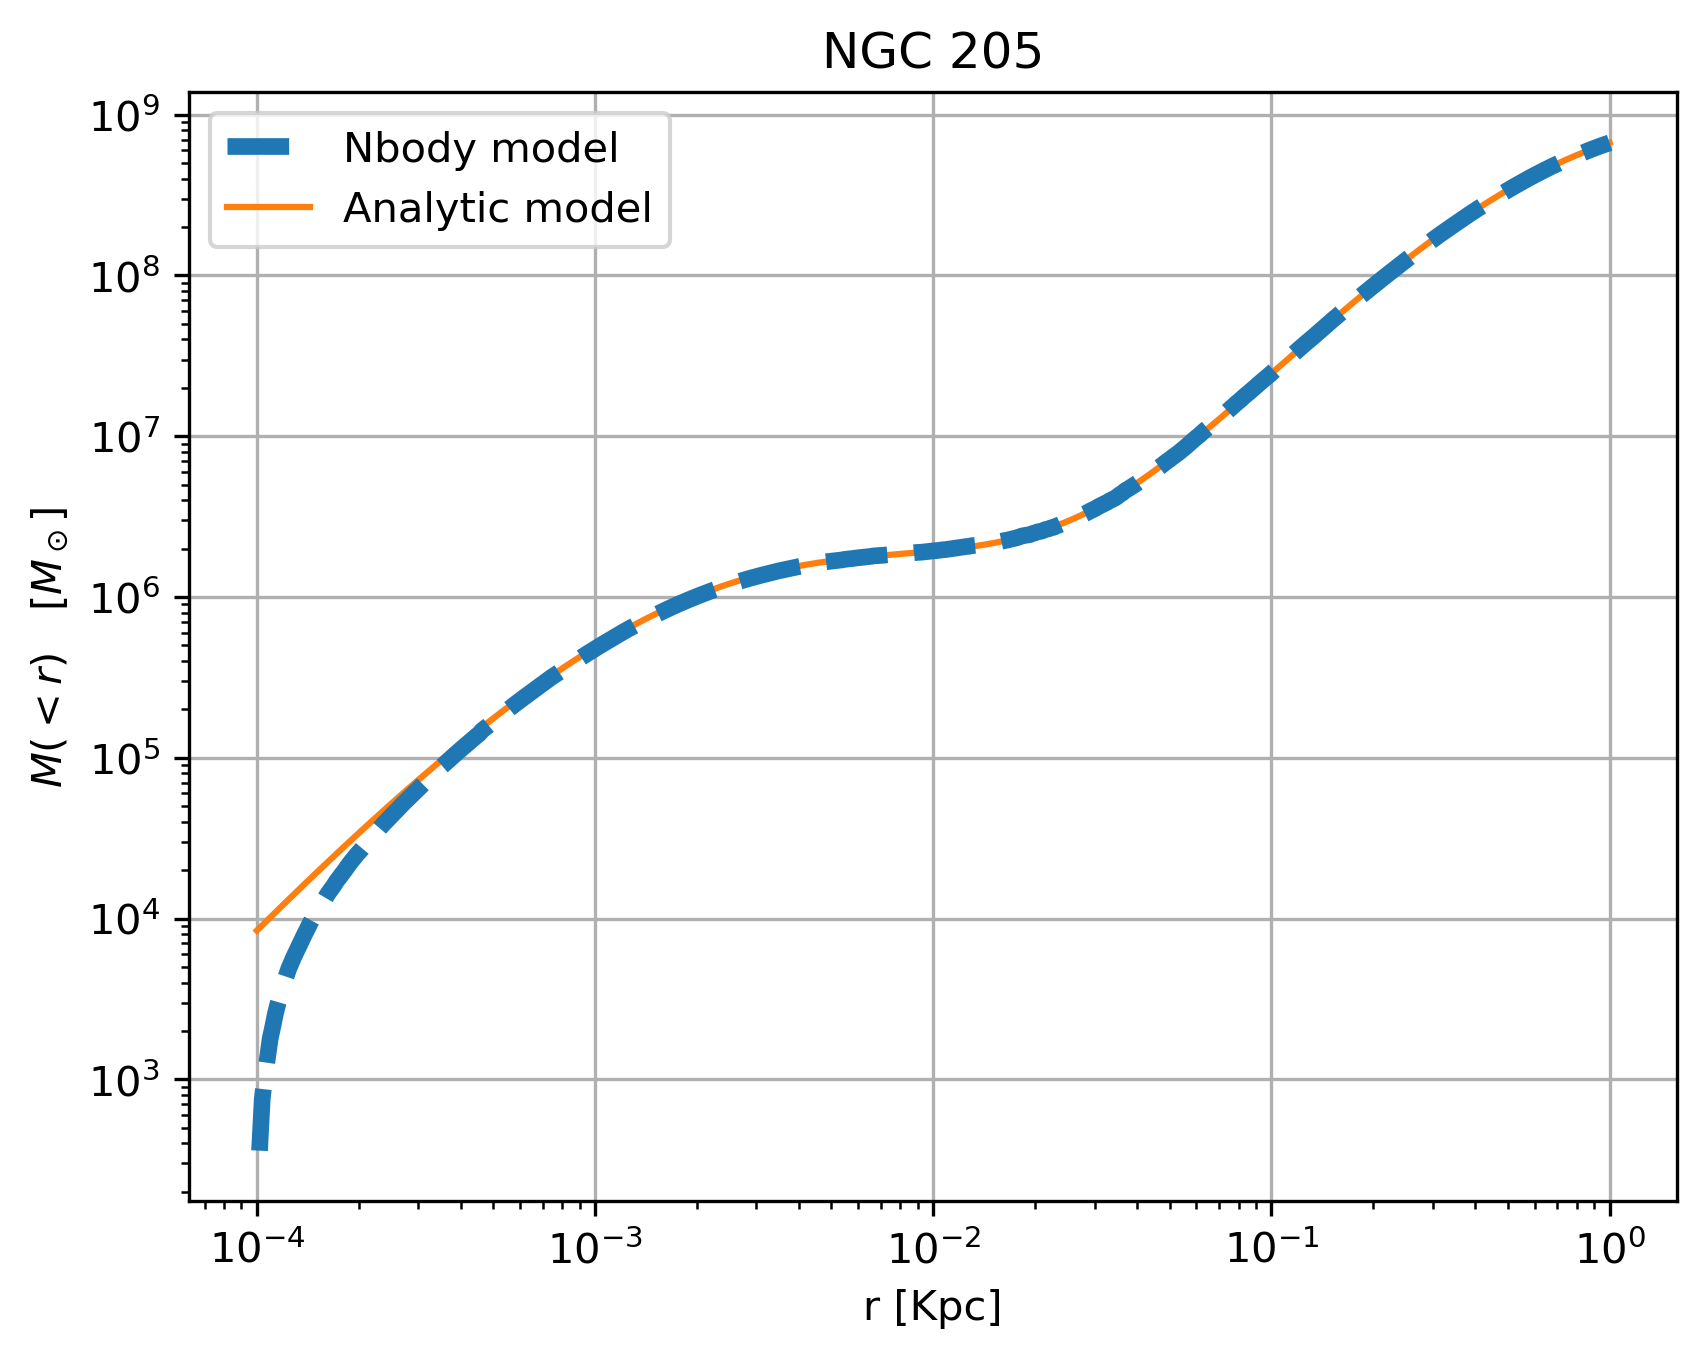
\includegraphics[width=\linewidth]{NGC205_mass_Nbody_vs_analytic.png}
\caption{B}
\end{subfigure}

\caption{aaa}
\label{NGC205 density and mass plot Nbody vs analytical}
\end{figure}

COM data:
\begin{itemize}
    \item position:
    \item velocity:
\end{itemize}



Numerically is found $r_{half}=...=... R_{eff}$.

\begin{figure}
    \centering
    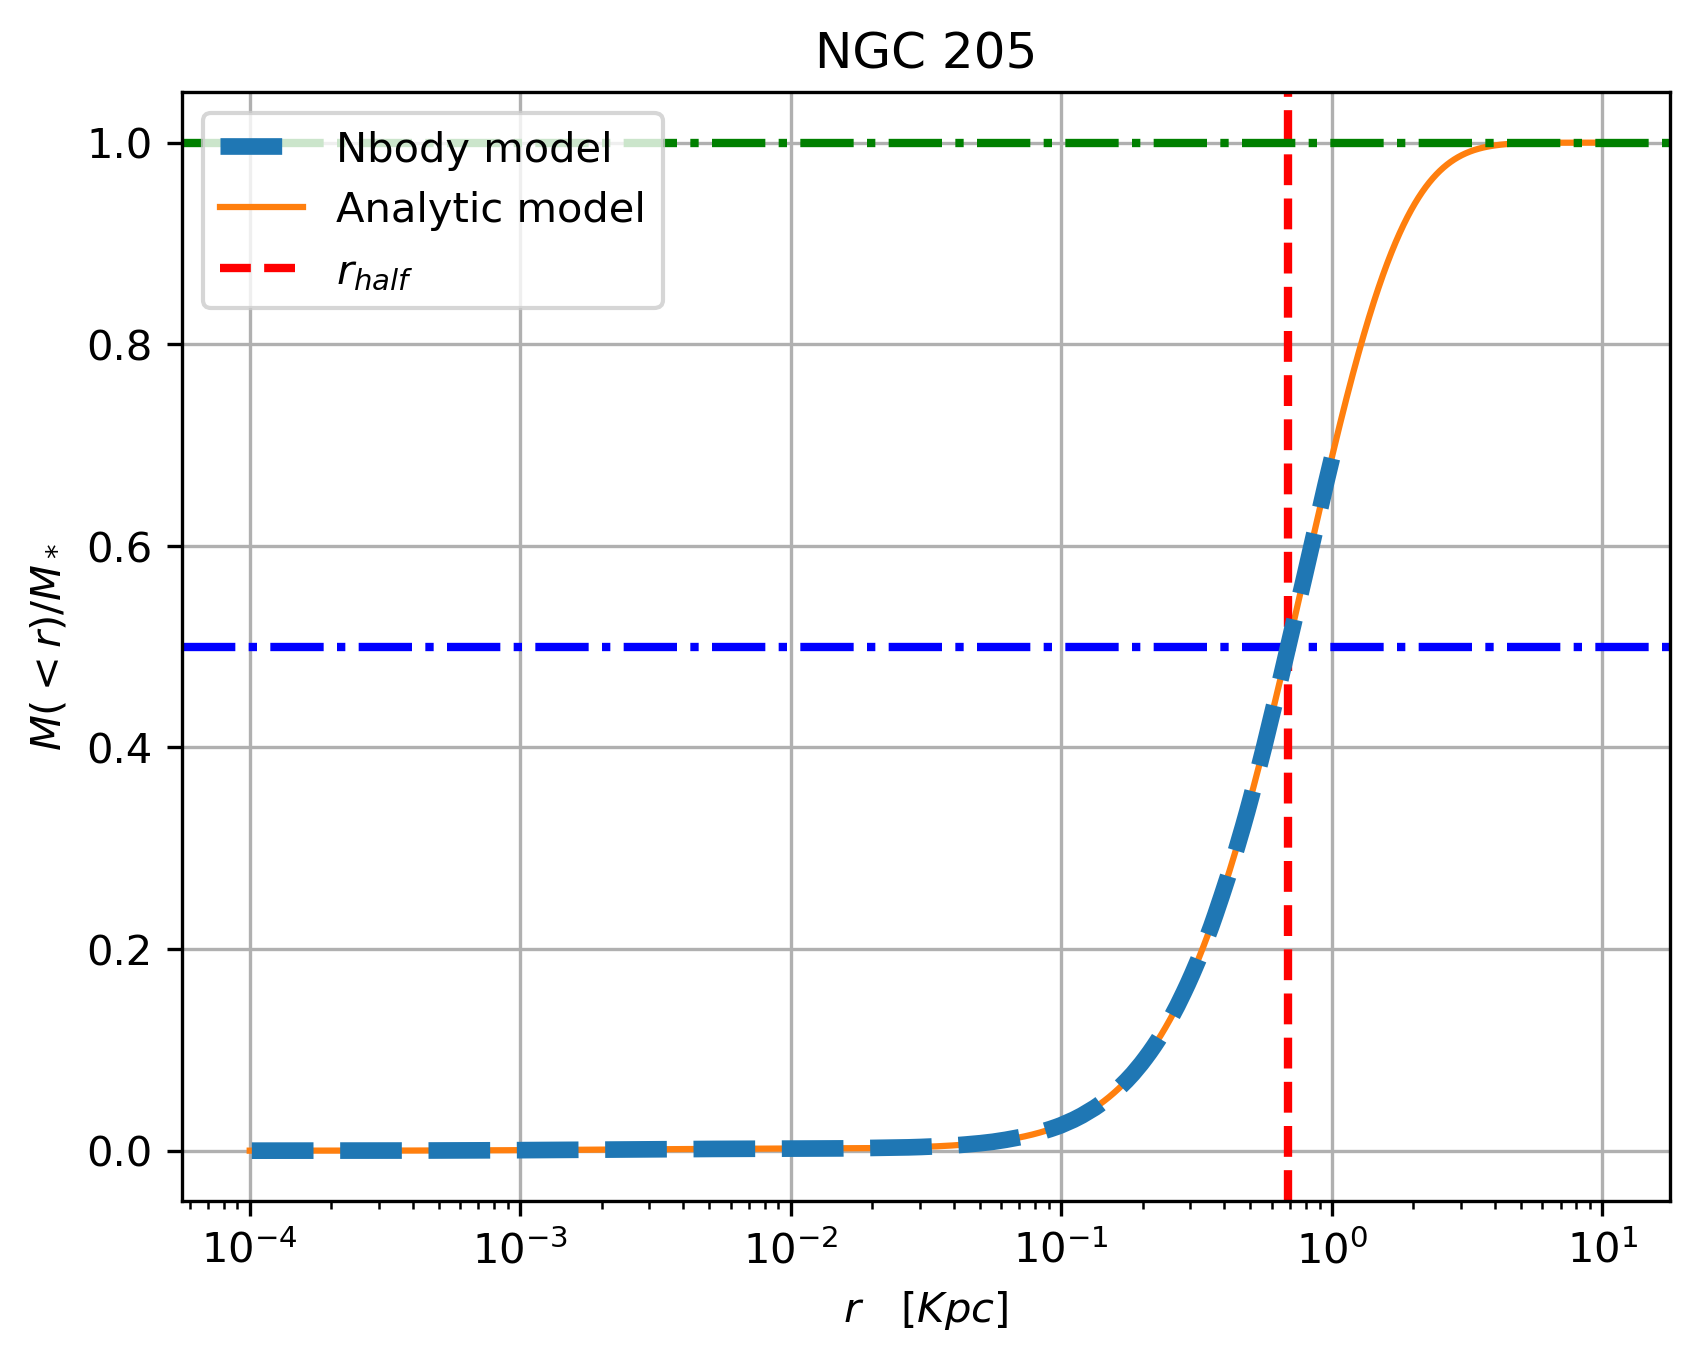
\includegraphics[width=0.5\linewidth]{NGC205_halfmass.png}
    \caption{aaa}
    \label{NGC205_halfmass}
\end{figure}
Yet, we get $t_{dyn}=...$, which agrees within $x\%$ the estimate obtained from the Analysis
tool provided by OpOpgadget, which measures this quantity directely from the generated model.
\\Waiting for evolution with Ketju.

\newpage
\subsection{NCG 5206 N-body Initial Conditions}
\section{Ketju Numerical Simulations}

\newpage
Things done:
\begin{itemize}
 \item created double galaxy
 \item modified BHs position and velocity
 \item modified their position and velocity according to Nipoti paper $(r_{90})$
 \item built Hists to check position and velocity distribution
 \item verified dyn equilibrium
 \item computed the softening length in several ways
 \item computed dyn time
 \item ketju run
 \item BHs analysis with ketju-utils
 \item snapshot analysis with OpOpgadget
 \item method of shrinking spheres to get the density peak position
\end{itemize}




\appendix
\renewcommand{\cftchappresnum}{APPENDIX~}
\renewcommand{\cftchapnumwidth}{9em}

\chapter{Physics Equation}

\chapter{Numerical Methods}
\section{Runge-Kutta (4)}
Given the first order autonomous ODE 
\begin{equation}
    \frac{du}{dt}=f(u),
\end{equation}
the stability anylisis of RK (4) applied to this equation leads to the following stability criterion on the time step size when $f(u)=au$:
\begin{equation}\label{RK (4) stability}
    \Delta t \le \frac{2.79}{|a|}.
\end{equation}
A system of first order autonomous ODEs can be written in vectorial form as:
\begin{equation}
    \mathbf{u}'=\mathbf{f}(\mathbf{u}).
\end{equation}
At linear order, the stability analysis we are allowed to perform the stability analysis to the linearized system
\begin{equation}
    \delta \mathbf{u}'=\mathbf{J}\delta \mathbf{u},
\end{equation}
where $\lambda_i$ is the i-th eigenvalue of the jacobian matrix $\mathbf{J}=\partial \mathbf{f}/\partial \mathbf{u}$.\\In the eigenvectors frame, equations look like
\begin{equation}
    \delta u'_i=\lambda_i\delta u_i\qquad\forall i=1,N
\end{equation}
and according to Equation (\ref{RK (4) stability}), one would get 
\begin{equation}
    \Delta t_i \le \frac{2.79}{|\lambda_i|} \qquad \forall i=1,N.
\end{equation}
Therefore, for a system of N Equations, a proper choice of the time step should be
\begin{equation}
    \Delta t=\epsilon \cdot min\left \{\frac{2.79}{|\lambda_i|}\right\} \qquad \forall i=1,N
\end{equation}
with $\epsilon\le 1$.



\printbibliography


\end{document}
